\documentclass[12pt]{article}
\usepackage{epsfig}
\setlength{\textwidth}{6.75in}
\setlength{\textheight}{7.5in}
\newsavebox{\savepar}
\newenvironment{boxit}{
  \begin{minipage}[b]{1in}}
 {\end{minipage}\fbox{\usebox{\savepar}}}

\setlength{\hoffset}{0.0in}
\setlength{\voffset}{0.0in}
\setlength{\marginparsep}{0.0in}
\setlength{\headheight}{0.0in}
\setlength{\headsep}{0.0in}
\setlength{\topmargin}{0.5in}
\setlength{\textheight}{8.5in}
\setlength{\oddsidemargin}{-0.1in}
\setlength{\evensidemargin}{-0.1in}
\setlength{\marginparwidth}{0.0in}
\setlength{\textwidth}{6.5in}
\setcounter{secnumdepth}{4}
\usepackage[htt]{hyphenat}
\begin{document}
%\def\decaysto{\vbox{
%   \hbox{\raise.5ex\hbox{\vrule height10pt}
%   \kern-.4025em{$\rightarrow$}}}\kern0.8ex}

\begin{center}
{\Large{\bf CMS Pixel Online Software and Calibrations}}
\end{center}
\begin{center}
\vskip 0.5cm
Anders Ryd ({\it anders.ryd@cornell.edu})\\
Steve Stroiney ({\it srs63@lepp.cornell.edu})\\
Souvik Das ({\it sd259@cornell.edu}) \\
Karl Ecklund ({\it Karl.Ecklund@cern.ch})\\
Josh Thompson ({\it joshua.thompson@cern.ch}) \\
Ben Kreis ({\it benjaminkreis@gmail.com})\\
% (If you make contributions to this document, please add your name above.)\\
\today \\
\end{center}

\begin{abstract}
Pixel Online Software (POS) is the online data acquisition software for the
CMS Pixel Detector that orchestrates its operation, calibration and monitoring.
This Note describes the structure and installation of this software.
It also documents the algorithms used to calibrate the detector. This document currently
serves both as a Reference Manual for and a User's Guide to POS.

%We might want to separate out the different components later.
\end{abstract}

\newpage

\tableofcontents

\newpage


\section{Introduction}

This note describes the design and implementation of
Pixel Online Software (POS). POS is used for controlling and calibrating the CMS pixel
detector. In particular, it performs the following functions:
\begin{itemize}
\item Configuring the detector
\item Performing online calibrations
\item Analyzing calibration data in online farm (CMSSW)
\item Monitoring the detector during data taking
\end{itemize}

In Section~\ref{sect:overview} the main software components
are introduced. Next the software organization is discussed.
In Section~\ref{sect:swcomponets} the different software components
are discussed in more detail. In Section~\ref{sect:calib} the
different calibrations are described. Other information about
Pixel Online Software is available at the pixel online
software wiki pages~\cite{poswiki}.

\section{Pixel DAQ System}

The intention of this section it to give an overview of
the CMS pixel DAQ system. For more details the reader
can follow the references given in the text. But the
introduction given here should be sufficient to understand
the main goals of POS.

\subsection{Overview of DAQ components}

The CMS pixel DAQ system consists of a number of
components as illustrated in Fig.~\ref{fig:daqcomponents}.
This figure is specific to the FPix detector, but the
modification for the BPix are minor and not really
relevant to the discussion here unless otherwise
mentioned. Starting from the detector itself we have the
Read Out Chip (ROC)~\cite{ROC} and the Token Bit Manager
(TBM)~\cite{TBM}. Some properties of the ROC are described
below as needed to understand the calibrations. The
ROC reads out 4,160 pixels and the TBM coordinates
the communication with a group of 8 to 24 ROCs.
The TBM is electrically connected to the portcard via
extension cables $\approx 2$ feet in length.

The portcard receives and sends optical signals to the
Front-End Controller (FEC) and Front-End Driver (FED)
respectively. The FEC is used to program the TBM
and ROCs and the data read out from the detector is
send to the FED to be digitized. The portcard is
home to several discrete components. We have the
Digital Opto-Hybrid (DOH) that receives data from
the FEC and the Analog Opto-Hybrid (AOH) that
transmits data to the FED. On the portcard we
have in addition the (t)PLL, Delay25, and gatekeeper
chips.

Of particular interest is the Delay25 chip. The communication
to the portcard via the DOH is done at 40MHz on a serial
line. We have a clock line and the data line (and return clock
and return data). In order to have this communication
working the timing between the clock and data lines must
be right. The purpose of the Delay25 chip is to adjust
delays to make this communication work. The setting of the
parameters on the Delay25 chip as well as the other components
on the portcard is done using the I2C protocol from the
CCU. The CCU is again controlled from a Tracker FEC (TkFEC).

\begin{figure}[h]
\begin{center}
 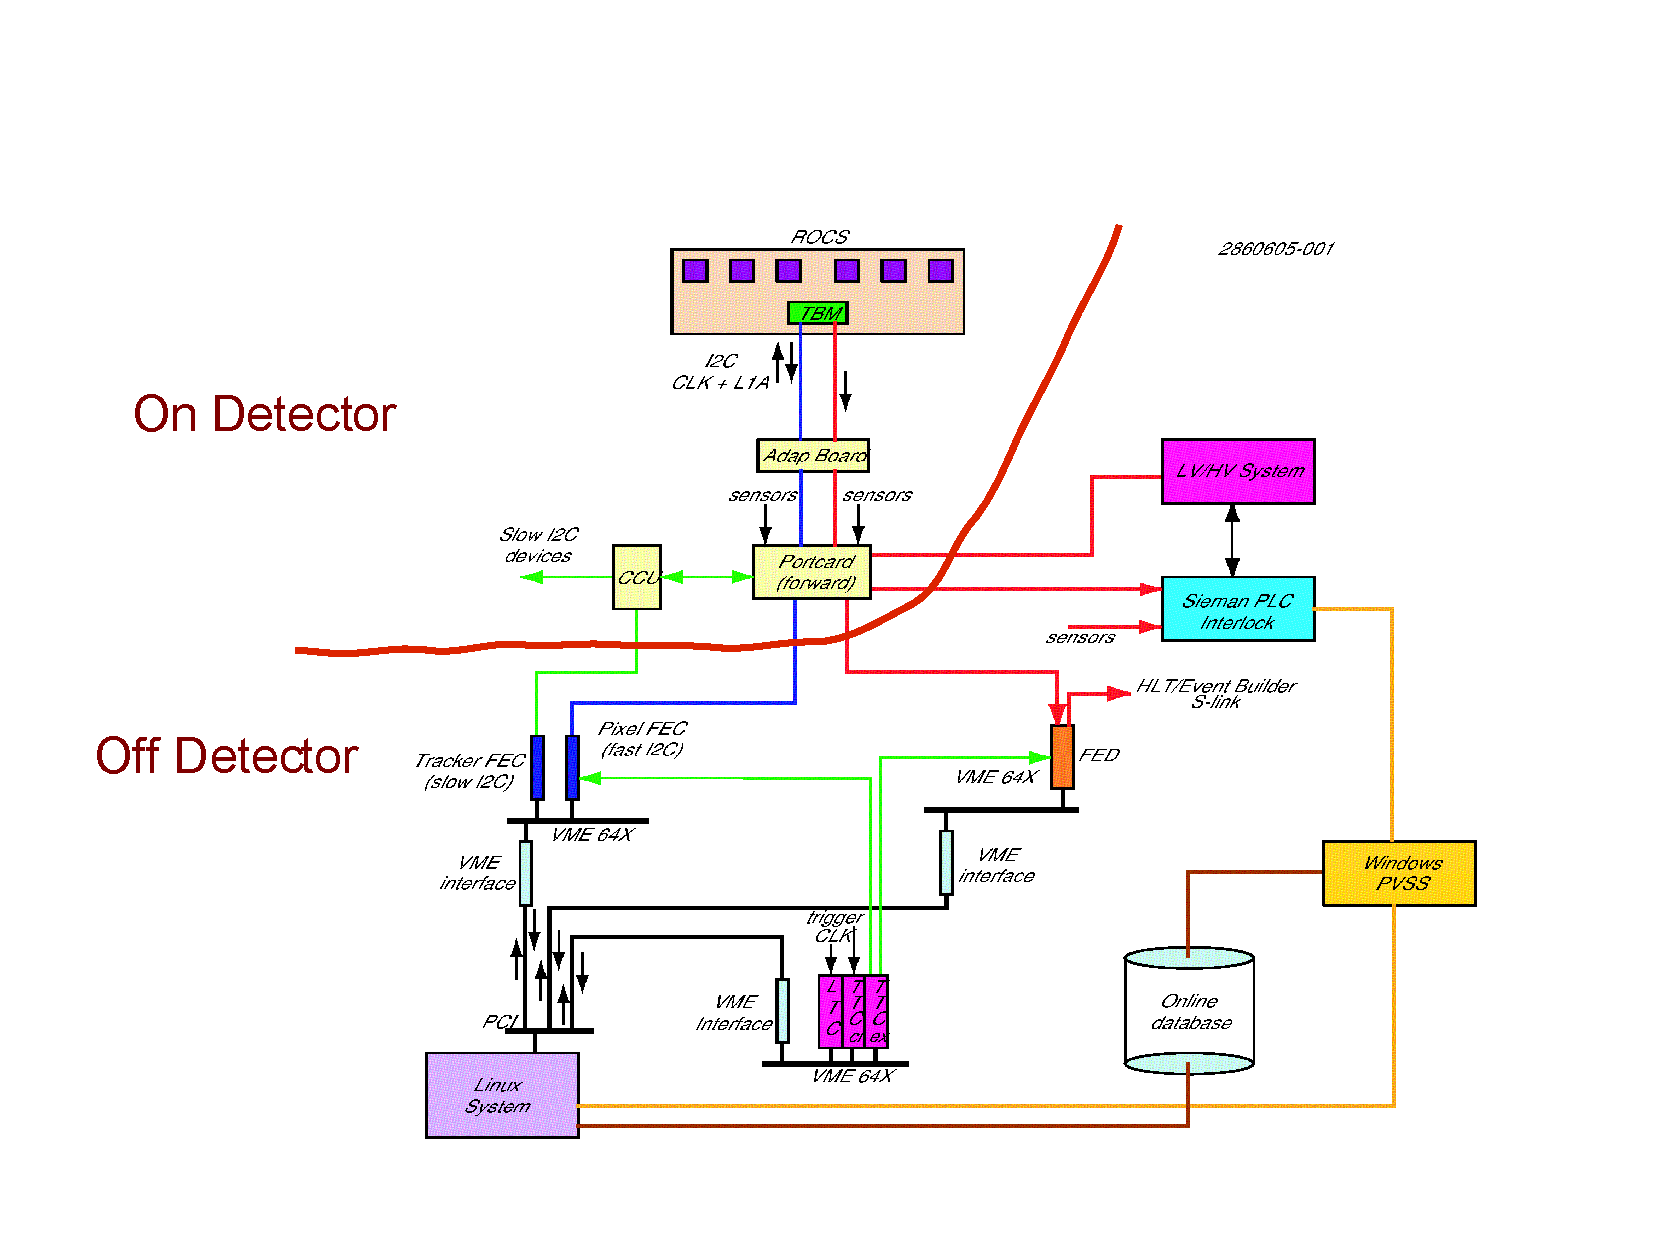
\includegraphics[width=0.99\textwidth]{2860506-001}
\end{center}
\caption{The main components in the CMS pixel DAQ system. }
\label{fig:daqcomponents}
\end{figure}

\subsubsection{The Read Out Chip}

Each Read Out Chip (ROC)~\cite{ROC}, illustrated in Fig.~\ref{fig:ROC}, collates data from 52 $\times$ 80 = 4,160 pixels
and contains about 1.3 million transistors.
It amplifies and zero suppresses data using 4 trim bits
that specify a threshold for every pixel. The chip buffers hit data
until the trigger decision arrives. It is developed at PSI and manufactured by IBM~\cite{Barbero:2004}.

\begin{figure}[h]
\begin{center}
 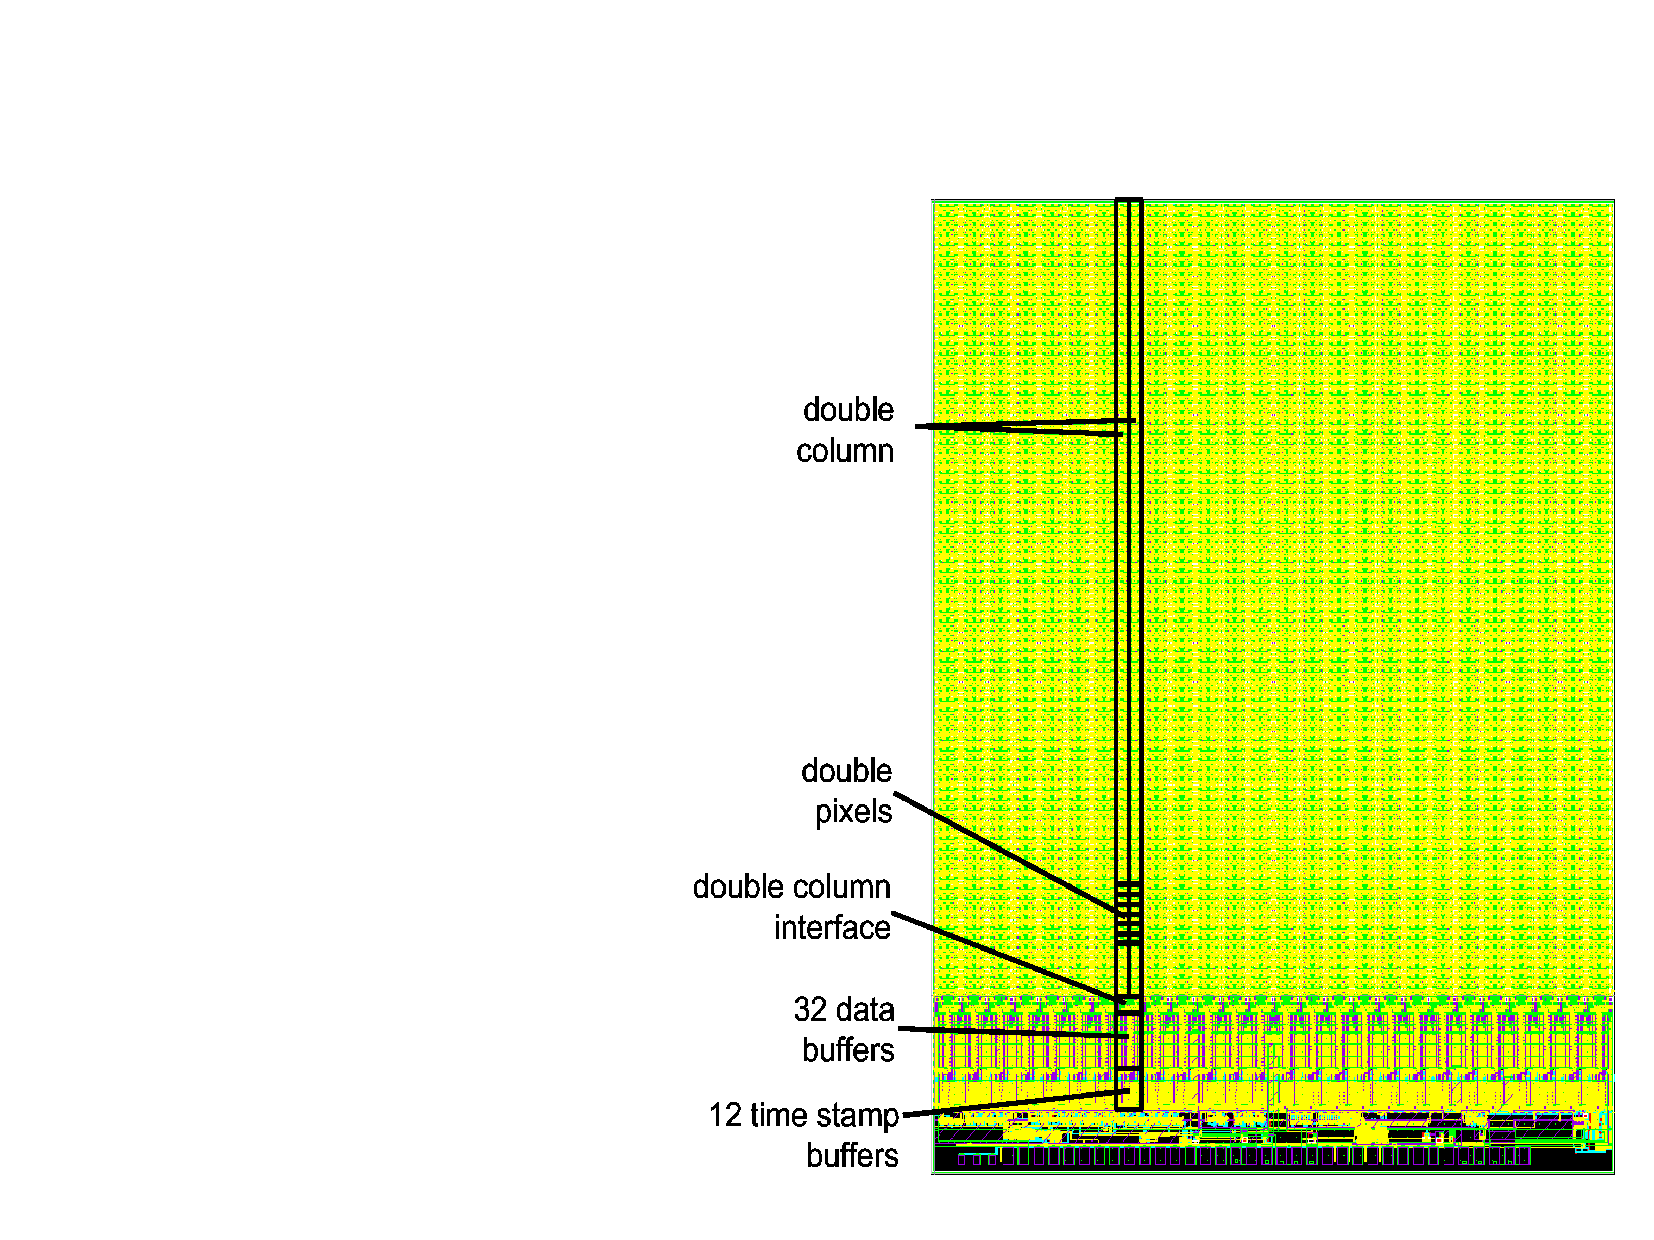
\includegraphics[width=0.45\textwidth]{ROC.pdf}
\end{center}
\caption{The Read Out Chip of the CMS Pixel Detector.}
\label{fig:ROC}
\end{figure}

For pixel hits to be read out, the following consecutive actions must take place.

\begin{itemize}

\item The accumulated charge in any of the pixels of the double column must exceed
a (programmable) threshold (trim-input to comparator). Then the corresponding time-stamp
(bunch crossing number) is written into the time-stamp buffer presently pointed at, and
the analog signals and the pixel addresses of all hit pixels are written into the next
free data buffers. This hit-recording into the time stamp and data buffers runs autonomously
and asynchronously in each double column of the chip, independently of the bunch crossing
clock. The recorded hit information must be kept in the buffers during the
latency time of the L1-trigger.

\item Hits in the column are validated by an external L1-trigger, by comparing their
corresponding time stamp with a counter running behind the bunch crossing counter by the trigger
delay, else the hits are cleared. If the hits in the column are validated, the value of a 4-bit
trigger counter is latched into the column periphery. The column is frozen and cannot record further
until reset after the readout of the triggered hits. Other (untriggered) columns remain active.

\item All frozen columns with the latched value of the trigger counter equal to the present value
of the token counter are set to the readout mode. Directly afterwards, the trigger counter is
incremented. The readout process starts when the token bit enters the chip. After a three bit chip
header is sent, each consecutive double column which is in the readout mode is read out and reset.
Just before the token leaves the chip, the token counter is incremented. A new token is sent
for each trigger and only data belonging to that trigger will be sent onto the readout bus,
even if more triggers arrive between a trigger and the corresponding token.

\end{itemize}

\subsubsection{The Token Bit Manager}

A Token Bit Manager (TBM) controls groups of 8 to 24 ROCs.
It distributes the clock and trigger signals.
It serializes analog readout using a token bit
passed from ROC to ROC. It is physically mounted next to the ROCs.
The TBM is developed at Rutgers.

\begin{figure}[h]
\begin{center}
 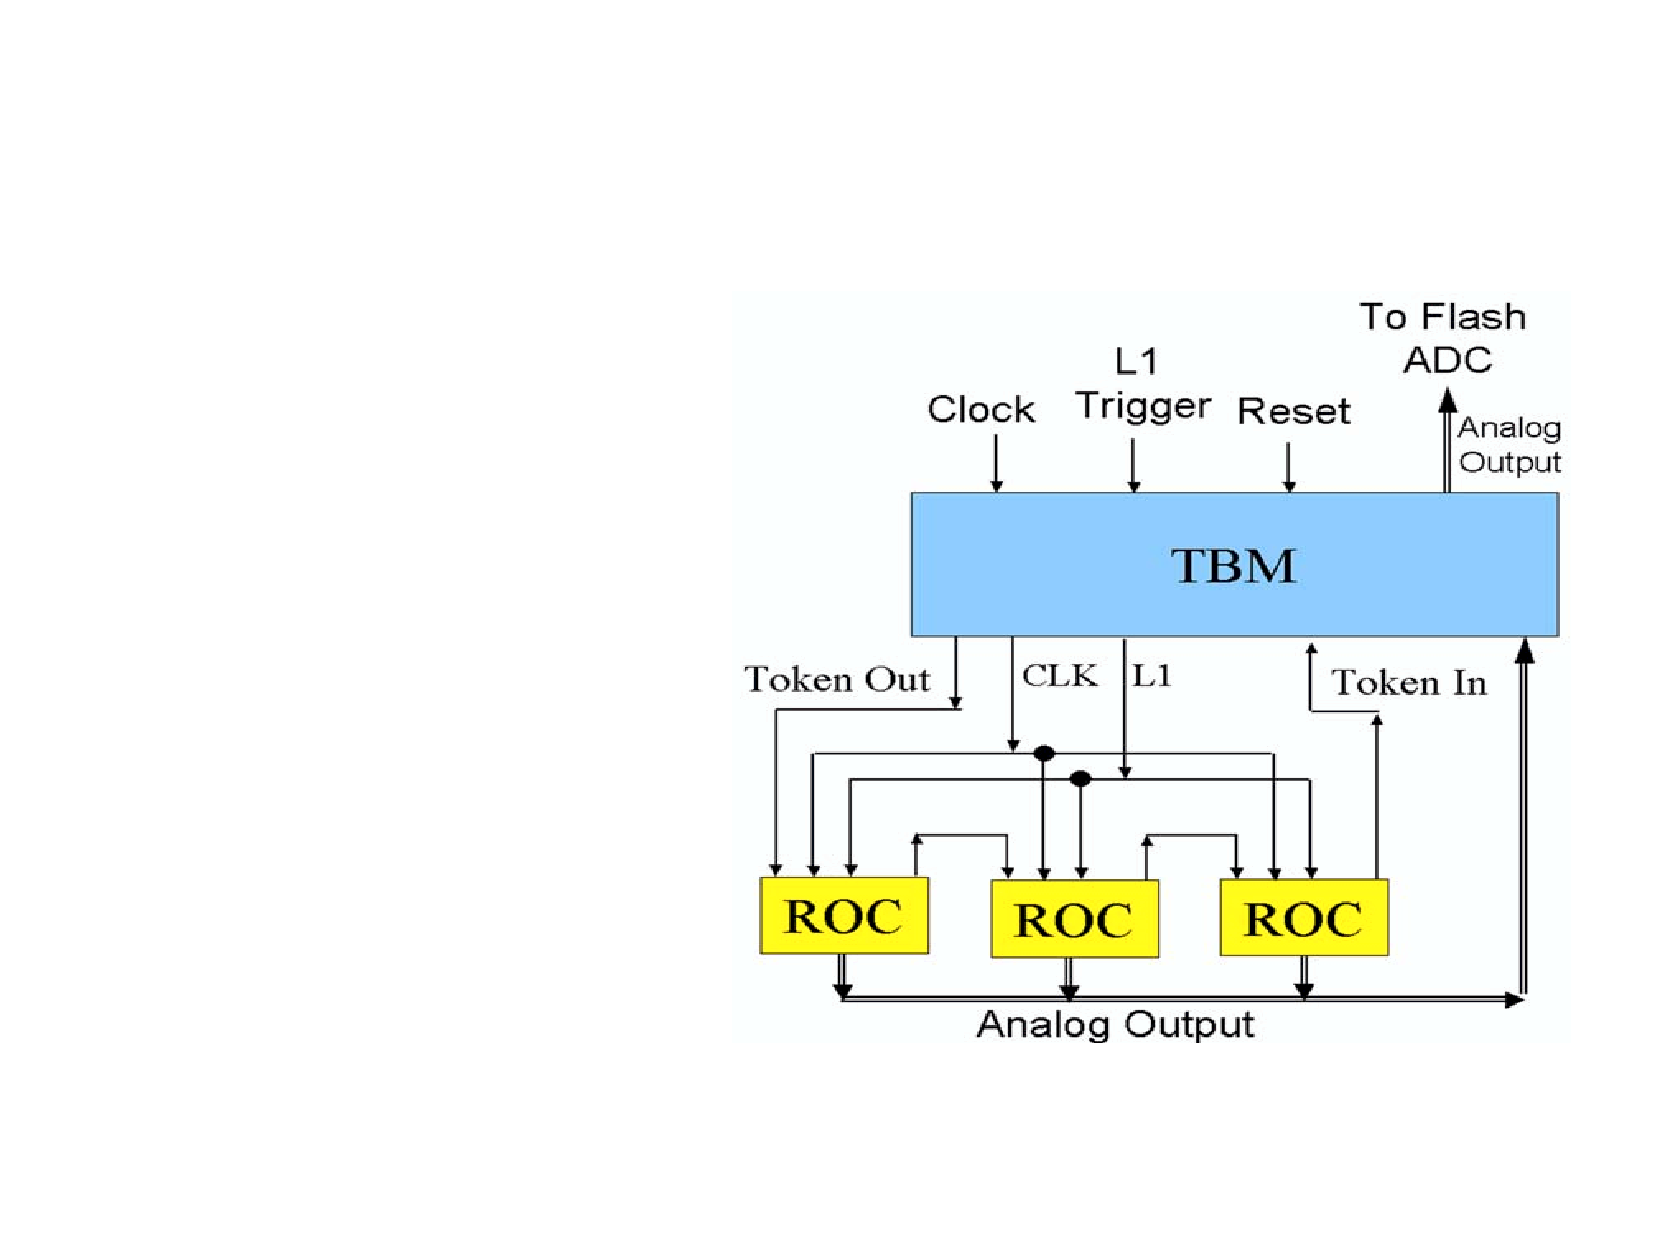
\includegraphics[width=0.45\textwidth]{TBM.pdf}
\end{center}
\caption{A schematic of how the Token Bit Manager reads out data from the ROCs.}
\label{fig:TBM}
\end{figure}

The principal functions of the TBM are the following.

\begin{itemize}

\item It controls the readout of the ROCs by initiating a token pass for each incoming
L1-trigger.

\item On each token pass, it writes a header and a trailer work to the data stream.

\item The header contains an 8-bit event number. The trailer contains an 8-bit error status.
These are transmitted in 2-bit analog encoded digital signals.

\item It distributes the L1-trigger and LHC Clock to the ROCs.

\item Each arriving L1-trigger is placed on a 32-deep stack awaiting its associated token pass.
Normally the stack is empty but is needed to accommodate high burst rates due to either noise,
high track density or trigger bursts. Only the first 16 triggers placed on the stack are passed
to the ROCs, and have an associated token pass. All others are marked in the trailer as a ``No
Token Pass" event. This is done to keep the DAQ synchronized, while speeding up the clearing of
the stack.

\end{itemize}

The TBM received 4 control signals: A 40 MHz clock synchronized to the CMS beam crossing, an active
low reset signal (which resets all control registers to an initial state), a serial line for
configuration settings, and a serial encoded trigger signal.

\subsubsection{The Pixel FED}

The Pixel Front End Driver (FED) is a VME module
with 36 optical inputs. It sits in the counting room and receives the analog output
of the ROCs via an optical fiber from the center of the CMS detector.
In order for the FED to decode and digitize this data, it has to have address levels
well calibrated, and this is one of the several tasks performed by the Pixel Online Software.
Internal timings of the FED also have to be calibrated within errors of a few nanoseconds,
and this is also accomplished using the POS. The output of the FED
is dispatched, in a binary format readable to the entire CMS experiment, via an S-Link.

\begin{figure}[h]
\begin{center}
 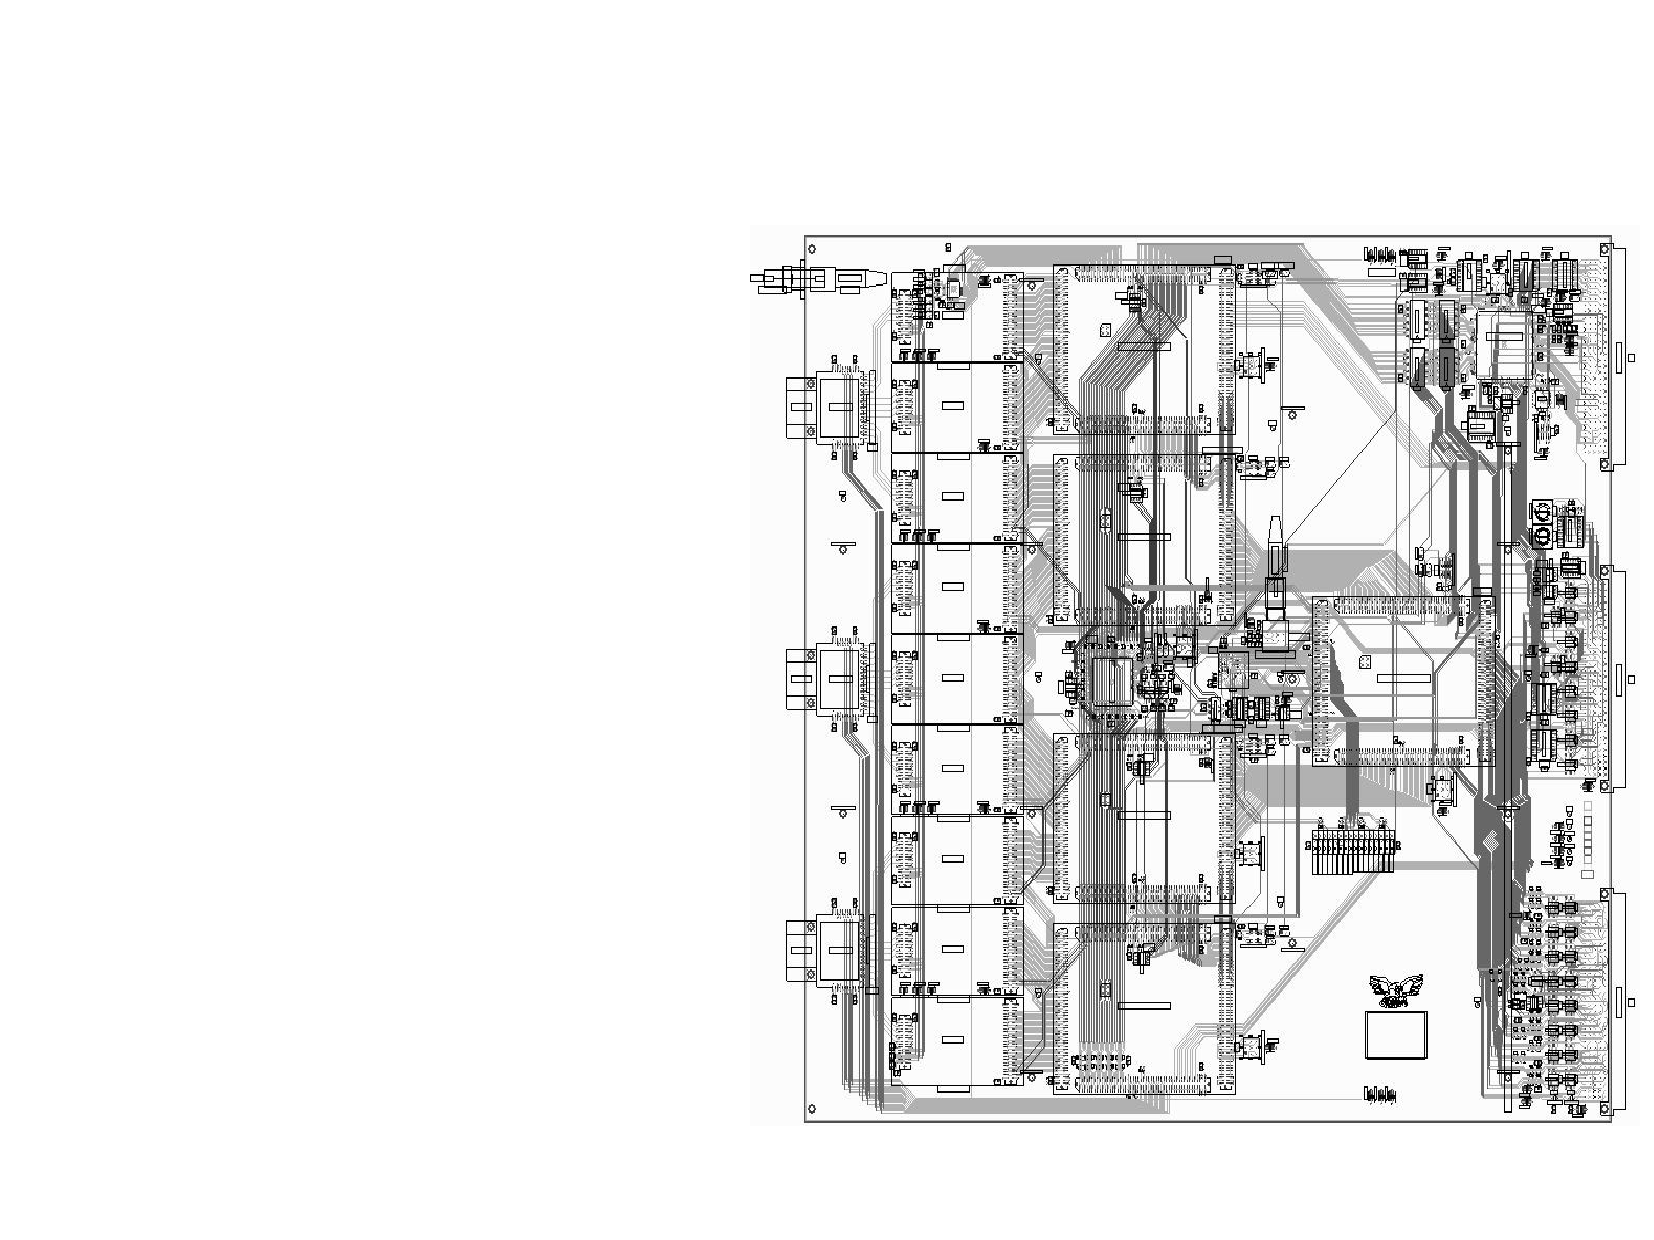
\includegraphics[width=0.45\textwidth]{pFED.pdf}
\end{center}
\caption{A schematic of the pixel FED.}
\label{fig:pFED}
\end{figure}

\subsubsection{The Pixel FEC}

The Pixel Front End Controller (FEC) sends triggers, clocks
and programming data to the ROCs. For the pixel detector,
we use a one-way `fast' I2C protocol to send this data.
We need to send 1 byte of data per pixel, or 66 MB of data
for the entire detector. For this, we use a 40 MHz serial line,
and this calls for timing calibrations in order to enable downloads.

\begin{figure}[h]
\begin{center}
 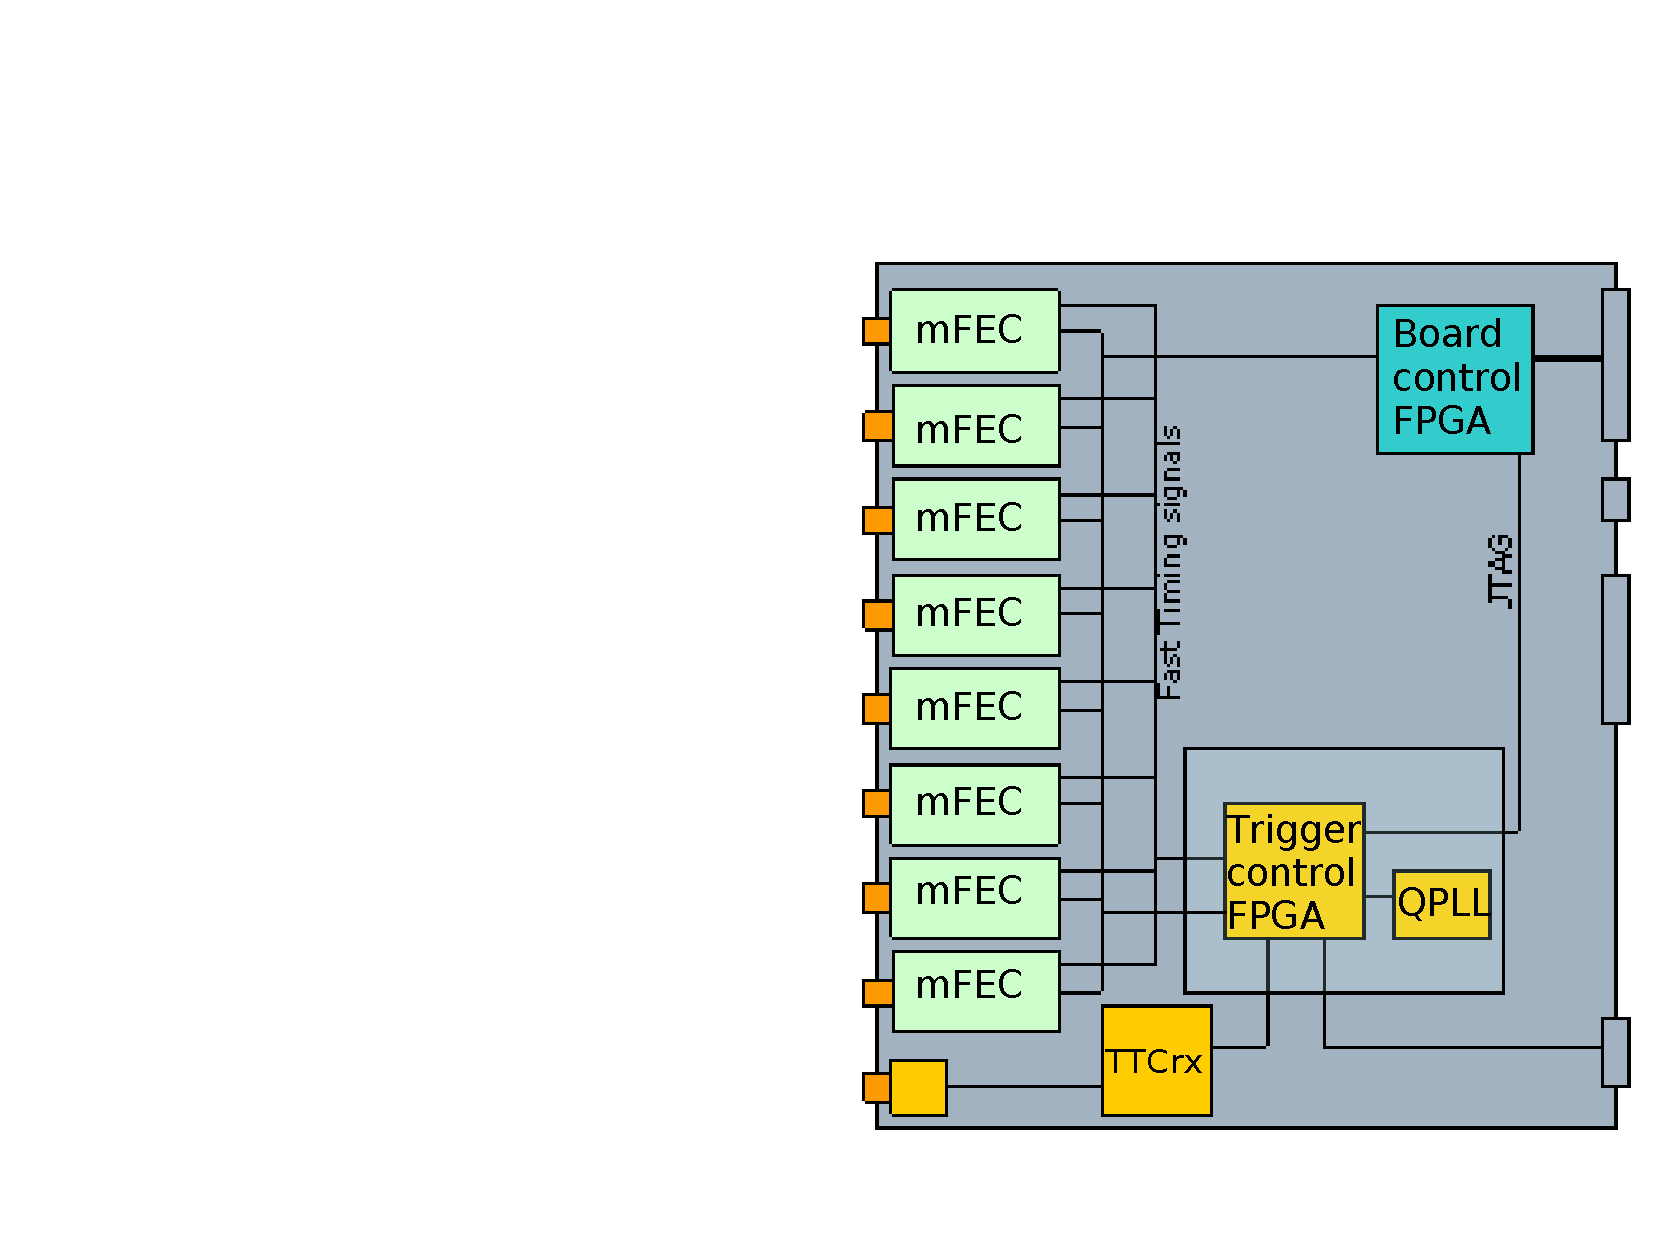
\includegraphics[width=0.45\textwidth]{pFEC.pdf}
\end{center}
\caption{A schematic of the pixel FEC.}
\label{fig:pFEC}
\end{figure}

\subsection{Installation at P5}

Table~\ref{tab:P5PCs} lists the online PCs that we have at P5
for Pixel Online Software. Table~\ref{tab:FpixFED} lists the FED boards
and their locations in the VME crate within the CMS Counting Room. The slots
and the VME addresses are also provided. Similarly, we list the FEC boards
and their locations in Table~\ref{tab:FpixFEC}. The CCU connections in the Counting
Room is shown in Table~\ref{tab:FpixCCU}.

\begin{table}
\centering
\caption{Pixel online PCs at P5}
\label{tab:P5PCs}
\resizebox{\textwidth}{!}{
\begin{tabular}{lcccccccc}
\hline
\hline
Slot in rack & Node name     & Front & Label & Size & Function        & Comments     & OS \\
\hline
          -  & vmepcs2b18-17 & Pixel & -  & ?U      &  Histoviewer    &              & SLC4 \\
          19 & vmepcs2b18-16 & Pixel & 1/10  & 1U   &  VME/S1G01i     & BPix FECs    & SLC4 \\
          17 & vmepcs2b18-15 & Pixel & 10/10 & 1U   &  VME/S1G01e     & FPix FECs    & SLC4 \\
          16 & vmepcs2b18-14 & Pixel & 9/10  & 1U   &  VME/S1G04e     & BPix FEDs do & SLC4 \\
      14/15  & vmepcs2b18-13 & Pixel & 8/10  & 2U   &  VME/S1G04i     & BPix FEDs up & SLC4 \\
          13 & vmepcs2b18-12 & Pixel & 7/10  & 1U   &  VME/S1G03i     & FPix FEDs    & SLC4 \\
          12 & vmepcs2b18-11 & Pixel & 6/10  & 1U   &  PixelSuperFPix & FPix Supv.   & SLC4 \\
          11 & vmepcs2b18-10 & Pixel & 5/10  & 1U   &  PixelSuperBPix & BPix Supv.   & SLC4 \\
          10 & vmepcs2b18-09 & Pixel & 4/10  & 1U   &  DCS            & Fpix daq     & Win \\
           9 & vmepcs2b18-08 & Pixel & 3/10  & 1U   &  DCS/Siemens    &              & Win \\
           8 & vmepcs2b18-07 & Pixel & 2/10  & 1U   &  DCS/CAEN       &              & Win \\
             & vmepcs2b16-10 &       &       &      &  TTC+LTC Supv.  & TTC+LTC      & SLC4 \\
             &  cmsrc-pixel  &       &       &      &  L1 FM          & Pixel FM     & SLC4 \\
             &fmmpc-s1d12-08 &       &       &      &  FMM PC         & FMM PC       & SLC4 \\
             &  cmspsx       &       &       &      &  PSX server     & PSX server   & SLC4 \\
             &  srv-c2c02-05 &       &       &      &  DB server      &              & SLC4 \\
             &  srv-c2c02-06 &       &       &      &  DB server      &              & SLC4 \\
\hline
\hline
\end{tabular}
}
\end{table}

\begin{small}
\begin{table}
\centering
\caption{FED connections for FPIX}
\label{tab:FpixFED}
\resizebox{\textwidth}{!}{
\begin{tabular}{llcccclc}
\hline
\hline
Rack   & Crate   & Slot & VME addr.  & Channels & FED id & Name(Official) & Name(Construction) \\
\hline
S1G03  & upper   & 6    & 0x13000000 &  13-24   & 33     & BpO\_D(1,2)\_BLD(1,2,3)    & HC+Z1 1.1 2.1\\
S1G03  & upper   & 6    & 0x13000000 &  1-12    & 33     & BpO\_D(1,2)\_BLD(4,5,6)    & HC+Z1 1.2 2.2\\
S1G03  & upper   & 7    & 0x14000000 &  13-24   & 34     & Bp0\_D(1,2)\_BLD(7,8,9)    & HC+Z1 1.3 2.3\\
S1G03  & upper   & 7    & 0x14000000 &  1-12    & 34     & Bp0\_D(1,2)\_BLD(10,11,12) & HC+Z1 1.4 2.4\\
\hline
S1G03  & upper   & 5    & 0x12000000 &  1-12    & 32     & BpI\_D(1,2)\_BLD(1,2,3)    & HC+Z2 1.4 2.4\\
S1G03  & upper   & 5    & 0x12000000 &  13-24   & 32     & BpI\_D(1,2)\_BLD(4,5,6)    & HC+Z2 1.3 2.3\\
S1G03  & upper   & 8    & 0x15000000 &  1-12    & 35     & BpI\_D(1,2)\_BLD(7,8,9)    & HC+Z2 1.2 2.2\\
S1G03  & upper   & 8    & 0x15000000 &  13-24   & 35     & BpI\_D(1,2)\_BLD(10,11,12) & HC+Z2 1.1 2.1\\
\hline
S1G03  & upper   & 11   & 0x17000000 &  13-24   & 37     & BmI\_D(1,2)\_BLD(1,2,3)    & HC-Z1 1.1 2.1\\
S1G03  & upper   & 11   & 0x17000000 &  1-12    & 37     & BmI\_D(1,2)\_BLD(4,5,6)    & HC-Z1 1.2 2.2\\
S1G03  & upper   & 12   & 0x18000000 &  13-24   & 38     & BmI\_D(1,2)\_BLD(7,8,9)    & HC-Z1 1.3 2.3\\
S1G03  & upper   & 12   & 0x18000000 &  1-12    & 38     & BmI\_D(1,2)\_BLD(10,11,12) & HC-Z1 1.4 2.4\\
\hline
S1G03  & upper   & 10   & 0x16000000 &  1-12    & 36     & BmO\_D(1,2)\_BLD(1,2,3)    & HC-Z2 1.4 2.4\\
S1G03  & upper   & 10   & 0x16000000 &  13-24   & 36     & BmO\_D(1,2)\_BLD(4,5,6)    & HC-Z2 1.3 2.3\\
S1G03  & upper   & 13   & 0x19000000 &  1-12    & 39     & BmO\_D(1,2)\_BLD(7,8,9)    & HC-Z2 1.2 2.2\\
S1G03  & upper   & 13   & 0x19000000 &  13-24   & 39     & BmO\_D(1,2)\_BLD(10,11,12) & HC-Z2 1.1 2.1\\
\hline
\hline
\end{tabular}
}
\end{table}
\end{small}

\begin{small}
\begin{table}
\centering
\caption{FEC connections for FPIX}
\label{tab:FpixFEC}
\resizebox{\textwidth}{!}{
\begin{tabular}{llllclc}
\hline
\hline
Rack   & Crate   & Slot & VME addr. & mFEC & Name(Official) & Name(Construction) \\
\hline
S1G01  & middle  & 5    & 0x28000000 & 3    & BpO\_D(1,2)\_BLD(1,2,3)    & HC+Z1 1.1 2.1\\
S1G01  & middle  & 5    & 0x28000000 & 4    & BpO\_D(1,2)\_BLD(4,5,6)    & HC+Z1 1.2 2.2\\
S1G01  & middle  & 5    & 0x28000000 & 5    & Bp0\_D(1,2)\_BLD(7,8,9)    & HC+Z1 1.3 2.3\\
S1G01  & middle  & 5    & 0x28000000 & 6    & Bp0\_D(1,2)\_BLD(10,11,12) & HC+Z1 1.4 2.4\\
\hline
S1G01  & middle  & 5    & 0x28000000 & 8    & BpI\_D(1,2)\_BLD(1,2,3)    & HC+Z2 1.4 2.4\\
S1G01  & middle  & 5    & 0x28000000 & 7    & BpI\_D(1,2)\_BLD(4,5,6)    & HC+Z2 1.3 2.3\\
S1G01  & middle  & 5    & 0x28000000 & 2    & BpI\_D(1,2)\_BLD(7,8,9)    & HC+Z2 1.2 2.2\\
S1G01  & middle  & 5    & 0x28000000 & 1    & BpI\_D(1,2)\_BLD(10,11,12) & HC+Z2 1.1 2.1\\
\hline
S1G01  & middle  & 10   & 0x50000000 & 3    & BmI\_D(1,2)\_BLD(1,2,3)    & HC-Z1 1.1 2.1\\
S1G01  & middle  & 10   & 0x50000000 & 4    & BmI\_D(1,2)\_BLD(4,5,6)    & HC-Z1 1.2 2.2\\
S1G01  & middle  & 10   & 0x50000000 & 5    & BmI\_D(1,2)\_BLD(7,8,9)    & HC-Z1 1.3 2.3\\
S1G01  & middle  & 10   & 0x50000000 & 6    & BmI\_D(1,2)\_BLD(10,11,12) & HC-Z1 1.4 2.4\\
\hline
S1G01  & middle  & 10   & 0x50000000 & 8    & BmO\_D(1,2)\_BLD(1,2,3)    & HC-Z2 1.4 2.4\\
S1G01  & middle  & 10   & 0x50000000 & 7    & BmO\_D(1,2)\_BLD(4,5,6)    & HC-Z2 1.3 2.3\\
S1G01  & middle  & 10   & 0x50000000 & 2    & BmO\_D(1,2)\_BLD(7,8,9)    & HC-Z2 1.2 2.2\\
S1G01  & middle  & 10   & 0x50000000 & 1    & BmO\_D(1,2)\_BLD(10,11,12) & HC-Z2 1.1 2.1\\
\hline
\hline
\end{tabular}
}
\end{table}
\end{small}

\begin{small}
\begin{table}
\centering
\caption{CCU connections for FPIX}
\label{tab:FpixCCU}
\begin{tabular}{llcccc}
\hline
\hline
Rack   & Crate   & Slot & mFEC & Name(Official) & Name(Construction) \\
\hline
S1G01  &  middle & 18   &  8   & BpI            & HC+Z2 \\
S1G01  &  middle & 18   &  7   & BpO            & HC+Z1 \\
S1G01  &  middle & 18   &  6   & Bm0            & HC-Z2 \\
S1G01  &  middle & 18   &  5   & BmI            & HC-Z1 \\
\hline
\hline
\end{tabular}
\end{table}
\end{small}


\section{Pixel Online Software Overview}
\label{sect:overview}

The Pixel Online Software is based on the XDAQ toolkit and is a suite of applications. The
different XDAQ based components are shown in green in
Fig.~\ref{fig:components}. The top level application is the
PixelSupervisor. This application is responsible for the overall
coordination of the pixel DAQ. The PixelSupervisor talks to the
supervisors that directly control the hardware. For example
we have the PixelFECSupervisor that provides the interface to the
pixel FECs. Similarly the PixelFEDSupervisor controls FEDs.
In production at P5, there are multiple instances of the PixelFECSupervisor and
PixelFEDSupervisor; one per VME crate\footnote{The strip tracker
uses a design where there is one supervisor per VME board.}.

The PixelTKFECSupervisor controls the tracker FEC hardware. The
pixel system uses the tracker FEC hardware slow I2C to
initialize the fast I2C used for the download of most
configuration data.

The PixelTTCSupervisor controls the pixel TTC module used for trigger
and timing. Among other things the TTC module is used during
calibrations to generate triggers. In modern releases of the software,
the PixelTTCSupervisor has been deprecated in favor of the
TTCciControl, which is a standard package maintained by the TTC group.

The PixelLTCSupervisor is used for the local trigger control.

The various supervisors run as independent processes, or even on
different computers. Therefore, in order to communicate with each
other they must exchange messages on the network. This is done using
the SOAP protocol.

The Level 1 function manager (L1FM or FM) for the pixels is the
interface the pixel system has to the global run control (RCMS for
Run Control and Monitoring System). The FM is a java application.
It responds to requests from RCMS to change states in the
state diagram that describe the state of the DAQ system. This
state diagram is shown in Fig.~\ref{fig:l1fm}.  The pixel
FM is a relatively thin layer that basically just passes the state
changes on to the PixelSupervisor.

\begin{figure}
\begin{center}
 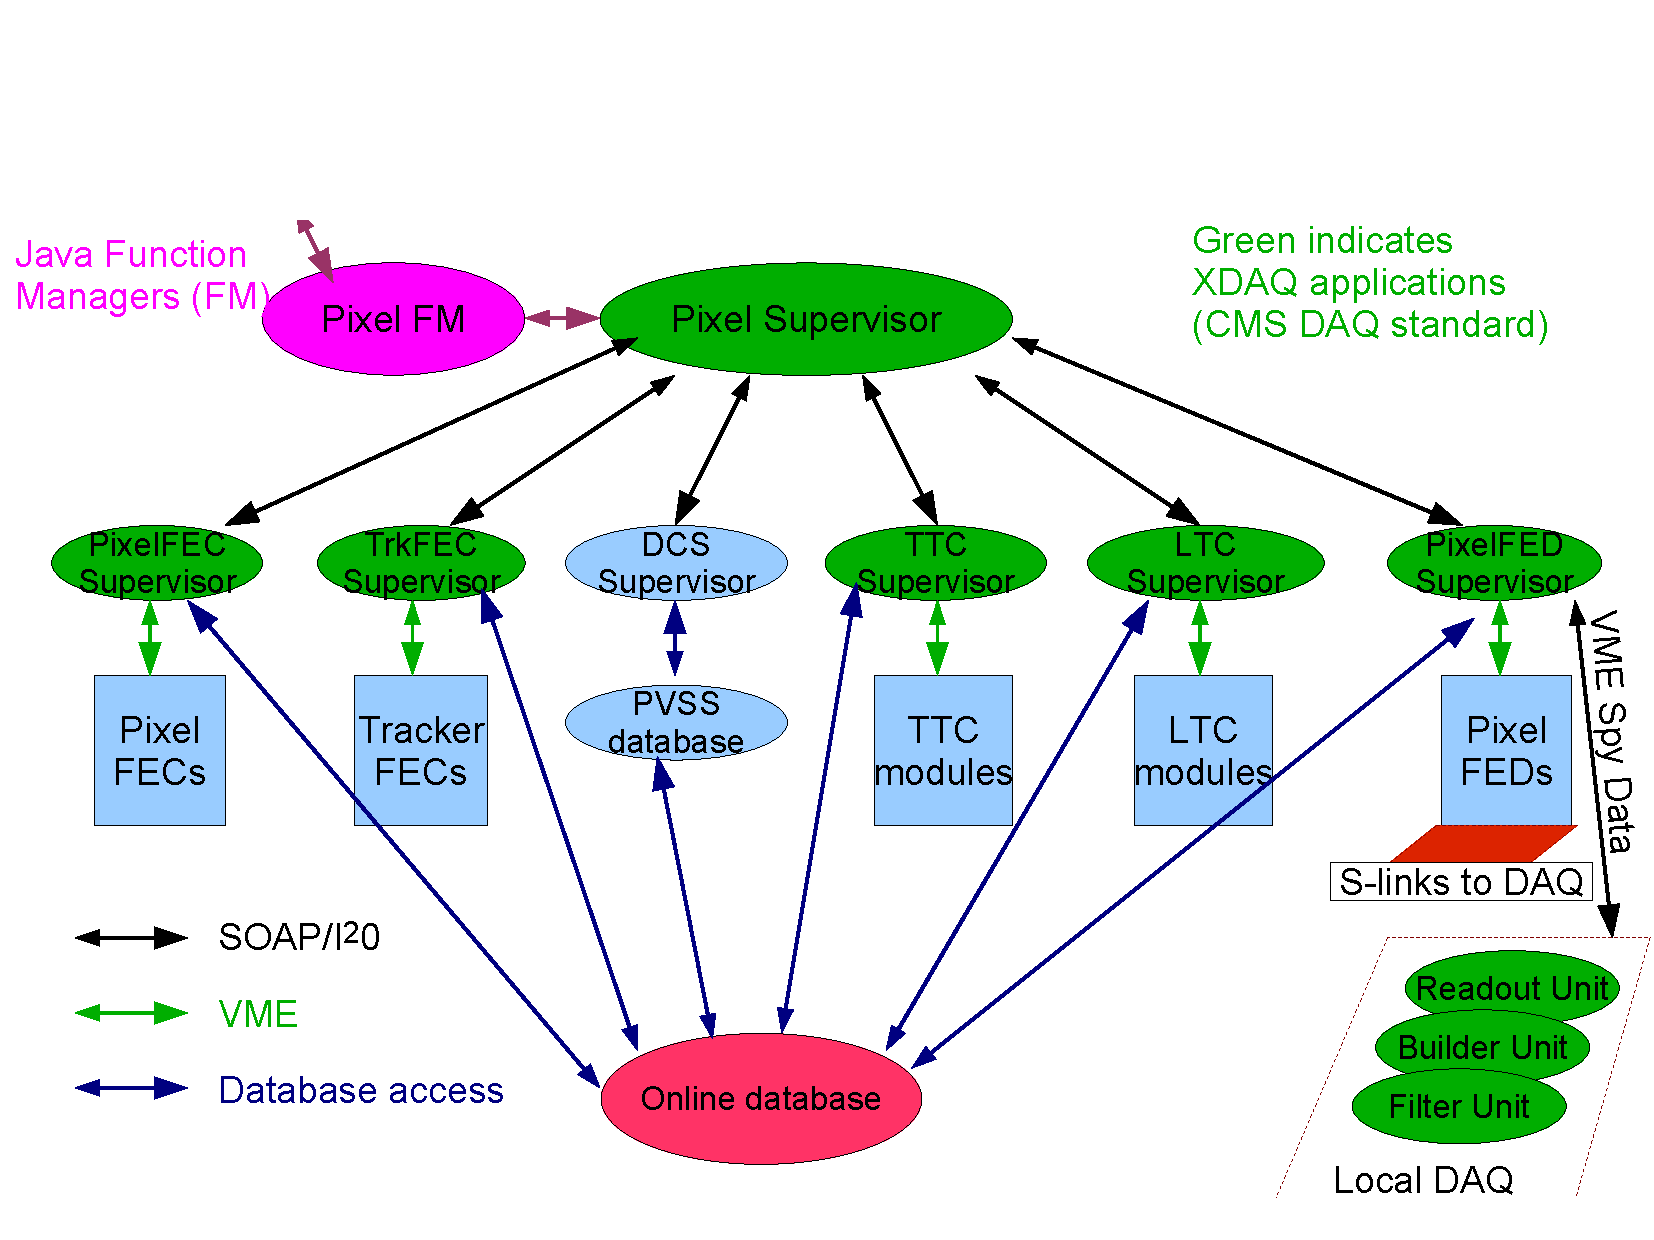
\includegraphics[width=0.99\textwidth]{POScomponents.pdf}
\end{center}
\caption{The different applications that compose the Pixel Online Software.}
\label{fig:components}
\end{figure}

\section{Package structure} \label{sect:swcomponets}

In the Pixel Online Software the code is distributed
among a number of packages. These packages are listed
here.
\begin{itemize}
\item PixelCalibrations
%\item PixelCalibrationInterface
\item CalibFormats/SiPixelObjects
\item PixelConfigDBInterface
%\item PixelDCSSupervisor
\item PixelDCSInterface
\item PixelFECInterface
\item PixelFECSupervisor
\item PixelFEDInterface
\item PixelFEDSupervisor
\item PixelFunctionManager
\item PixelLTCSupervisor
\item PixelSupervisor
\item PixelTKFECSupervisor
\item PixelTTCSupervisor\footnote{In use through tag {\tt POS\_3\_1\_2}; deprecated starting in {\tt POS\_3\_2\_0}.}
\item PixelUtilities
\end{itemize}
The package dependency tree is shown in Fig~\ref{fig:dependencies}.
The supervisor applications are at the top and depend on the
packages below. We should make sure that the dependencies
form a tree and not contain loops.

\begin{figure}
\begin{center}
 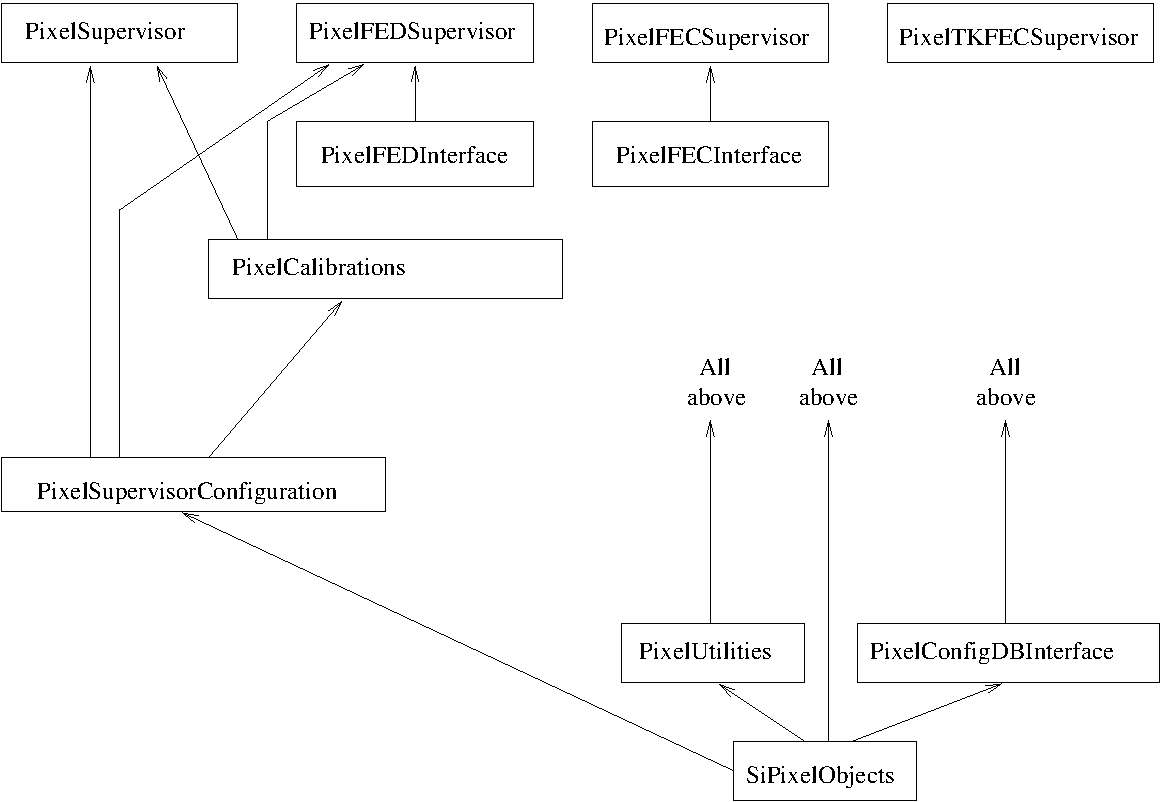
\includegraphics[width=0.99\textwidth]{package_dep.pdf}
\end{center}
\caption{The dependencies among the packages are indicated here.
At the top are Supervisor applications. }
\label{fig:dependencies}
\end{figure}



\subsection{Pixel Function Manager}
\label{sec:l1fm}
The Pixel Function Manager (the Level 1 Function Manager) acts as an interface between
Run Control (the Level 0 Function Manager) and POS. The Pixel Function Manager is a Java
application. It implements the state machine of
CMS~\cite{statemachine}. The Function Manager interacts
with the PixelSupervisor to carry out the
different tasks needed in state transitions of the
run control.

\begin{figure}
\begin{center}
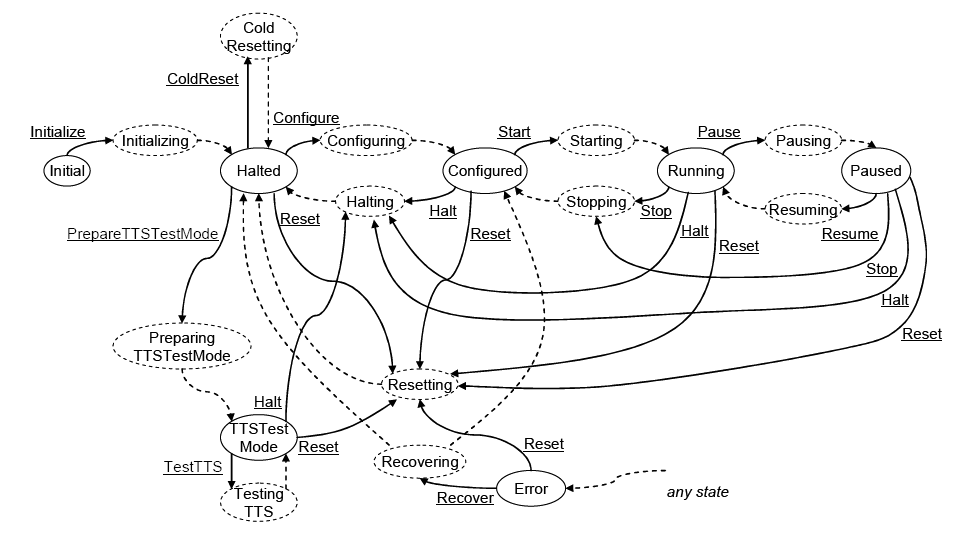
\includegraphics[width=0.99\textwidth]{l1fm_states.png}
\end{center}
\caption{The CMS finite state machine definition. Figure taken from Ref.~\cite{statemachine}.}
\label{fig:l1fm}
\end{figure}

\subsubsection{FSM Implementation Status}
The CMS Run Control finite state machine (FSM) is shown in
Fig.~\ref{fig:l1fm}. This model is implemented in the Pixel Function Manager,
 and also in the PixelSupervisor. The other
Supervisors implement portions of this model as required.
The FSM depicted in the figure is completely implemented in
the PixelSupervisor. The PixelSupervisor does
include transitions from any state into the ''Error'' state, and then
allows a ``Recover'' transition that returns the FSM to the ``Halted''
state.

\subsubsection{Control of the L1 Function Manager}

During global running, the L1 Function Manager (L1FM) is driven by the L0FM, which is
operated by central DAQ. The pixel user should not intervene via the
L1FM GUI, except to check its status.

During local running, the L1FM must be created via its GUI. State
transitions of the FSM can then be driven via the L1FM GUI. In
general, we drive the ``Initialize'' state transition via the GUI,
then drive subsequent state transitions directly from the
PixelSupervisor. However, in principle all transitions can be
initiated from the L1FM GUI.\footnote{In practice, this is only useful for simple tests of the L1FM to PixelSupervisor communication.}

\subsubsection{Outline of L1FM implementation}

The L1FM is created using the Create button in RCMS. This calls the
method of \texttt{PixelFunctionManager.java} called \texttt{
createAction()}.

After creation, transitions of the FM FSM are handled
by methods in {\tt PixelEventHandler.java}. Which method is triggered
depends on the transition, as defined by a table near the top of this
class. The names are fairly logical (for example, ``Initialize''
corresponds to the {\tt initAction} method and ``Configure''
corresponds to the {\tt configureAction} method). Inside each {\tt
fooAction} method are two blocks: one to handle objects of type {\tt
StateEnteredEvent} and one to handle objects of type {\tt
StateNotification}.

When an FSM transition ``foo'' is initiated by the L0FM or L1FM GUI,
we enter the {\tt StateEnteredEvent} block of {\tt fooAction}. This
block then contains the code to send a message to PixelSupervisor,
telling it to proceed with transition ``foo''. The L1FM then does
nothing while PixelSupervisor coordinates the necessary activities in
POS. When the transition is completed by the PixelSupervisor, it
passes a message back to the L1FM\footnote{This is implemented in
PixelSupervisor using the {\tt stateChanged} method of the {\tt
rcmsStateNotifier\_} object.}. This message triggers entry into the {\tt
StateNotification} block of {\tt fooAction}. If PixelSupervisor
reports that the transition was successful, this block moves the L1FM
FSM into the state ``foo''. If PixelSupervisor reports an error, this
block moves the L1FM FSM into state ``Error''. In this way, the L0FM
(central DAQ) learns whether the transition was successful.


\subsection{PixelSupervisor}

The PixelSupervisor is the top level Pixel Online Software application
in the Pixel Online Software. As described above it takes
commands from the function manager. There is one pixel
supervisor for the pixel online system.

\subsubsection{Functions}

The main function of the PixelSupervisor is to coordinate the
activities of the other supervisors, particularly during configuration
(see Sec.~\ref{sec:configuration}) and calibration (see
Sec.~\ref{sect:calib}). It is responsible for updating the
configuration database with new settings obtained by calibrations.

The PixelSupervisor also communicates the state of the pixel
XDAQ software (POS) to the Level 1 Function Manager (Sec.~\ref{sec:l1fm}).

\subsubsection{Interface}
The PixelSupervisor web GUI is an html page, which by default
refreshes every few seconds. It displays information about the current
configuration, or if it is not configured it allows the user to select
a possible configuration from a list and configure the detector using
that configuration.

The PixelSupervisor runs the JobControl Monitor, which is a utility
that periodically sends ``heartbeat'' SOAP messages to the JobControl
processes running on the various machines at P5. The PixelSupervisor
GUI uses the replies from these SOAP messages to display whether any of
the POS XDAQ processes has crashed, or whether any of the JobControl
processes themselves are unresponsive. (Note that we typically only
run JobControl at P5, so this feature is not available elsewhere.)

\subsection{PixelFECSupervisor}

The FEC Supervisor controls the pixel FECs. This means it is
responsible for loading the configuration parameters for the ROCs from
the configuration database and programming those parameters into the
detector.

\subsection{PixelFEDSupervisor}

The FED Supervisor controls and monitors the pixel FEDs.

%\subsection{PixelTTCSupervisor}



\section{Coding practices}

\subsection{Makefile}

The Pixel Online Software is built with a
Makefile located in each (sub)package. The
Makefile builds on the XDAQ tools. This
file should ideally be as short as possible
and use the functionallity in the XDAQ package.
You invoke the Makefile in each package by
doing a `make'. There is also a {\tt clean} target.

In addition to the package level makefiles
there is a top level makefile in the pixel
directory. This makefile allows you to build
all the XDAQ packages using {\tt make Set=pixel}.
You can also clean all packages using
{\tt make Set=pixel clean}.

\subsection{Include files}

Include statements should include the file path
starting from the project. For example you should do

\begin{verbatim}
#include "PixelCalibrations/include/PixelAOHBiasCalibration.h"
#include "CalibFormats/SiPixelObjects/interface/PixelCalibConfiguration.h"
\end{verbatim}

\subsection{CVS tags}

We create `official' tags of the form 'POS\_X\_Y\_Z',
e.g. 'POS\_2\_4\_5'. For every tag created, starting
with POS\_2\_5\_0, an entry should be made in the
file pixel/README that describes briefly the new
features in the tag.

\subsection{Building RPMs}

The building of RPMs should be straightforward. The
following steps are required.
\begin{itemize}
\item Prepare the code, update the README file, and VERSION file and
      commit and tag the code. The VERSION file contains the version
      of the RPM to build.
\item Invoke `make Set=pixel rpm' to build RPMs for all Pixel Online Software
      packages.
\item In the {\tt PixelUtilities} directory, invoke 'buildExternalRPMs.sh'
      to build RPMs for DiagSystem, TTCSoftware, and FecSoftwareV3\_0.
      At the end of building the external RPMs this script copies
      all RPMs to \$BUILD\_HOME/RPM\_X.Y.Z-V, where X, Y, Z, and V are
      the major version, minor version, patch, and build version,
      respectively.
\end{itemize}
The set of RPMs built can be tested (in the online environment) for
consistency by invoking the command 'rpm --test -Uvh *.rpm' in the directory
where all the RPMs are located.

Old RPMs can be cleaned out of the build area using the command 'make Set=pixel cleanrpm'.

\clearpage

\section{Configuration Data Management}

The next two sections describe a C++ interface
for configuration data management and the
different classes that are used to store this
information. For details of the organizational
details of the database structure, please refer
to the presentation:
\begin{verbatim}
http://indico.cern.ch/conferenceDisplay.py?confId=8768
\end{verbatim}

\section{Configuration Database Interface}

Since early summer 2006, we have used an interface for accessing
configuration data in the online software framework.
The access was originally file based, and has now (starting in 2009) been
supplemented with infrastructure to access an Oracle database. The
interface used is rather generic and the purpose of this document
is to write down the interface so that we can have a
clear separation between the database code and the applications
that use data from the configuration database.

First in Sect.~\ref{sect:cppinterface} we describe the C++ API.
The interface is defined in the class {\tt PixelConfigInterface}.
This interface is fully implemented in the {\tt PixelConfigFile}
implementation based on files.

In Sect.~\ref{sect:cmdline} a simple command line tool is described.
This tool is implemented through the C++ interface and should work
both for the file based and the final data base implementation.

Examples below use a few of the configuration data classes that are used.
% In Sect.~\ref{sect:configclasses} the full
% set of classes that are used to configure and control the pixel
% online software are discussed.

\subsection{C++ Configuration Data Access API}
\label{sect:cppinterface}

The class {\tt PixelConfigInterface} in the package
{\tt PixelConfigDBInterface} defines the interface for
access of configuration data. This interface is intended
to provide type safe access methods for retrieving and
storing configuration data.

\subsubsection{Retrieving data from the database}

The primary method for retrieving the data is
\begin{verbatim}
  template <class T>
  static void get(T* &pixelObject,
		  std::string path,
		  pos::PixelConfigKey key)
\end{verbatim}

The {\tt PixelConfigKey} is just an integer that holds the top
level configuration key to be used.
This interface returns a pointer to the data. The caller is assumed
to take ownership of the data and delete it.
The path is a 'secondary key'. It would allow us to store more than
one object of the same type in a given configuration. (In the file
based implementation this label is used to build the path to where the
file is stored.)
Below are a few examples of using this interface.
\begin{verbatim}

  PixelConfigKey theGlobalKey(5);

  PixelNameTranslation *theNameTranslation=0;
  PixelConfigInterface::get(theNameTranslation, "nametranslation/",
                     theGlobalKey);

  PixelDetectorConfig *theDetectorConfiguration=0;
  PixelConfigInterface::get(theDetectorConfiguration, "detconfig/",
                     theGlobalKey);

  PixelFECConfig *theFECConfiguration=0;
  PixelConfigInterface::get(theFECConfiguration, "fecconfig/",
                     theGlobalKey);

\end{verbatim}

These examples show how you extract objects for which there is only one
instance of for the
whole detector configuration. You pass in as the first argument a pointer. The
pointer will return 0 if the object was not successfully retrieved\footnote{We have now tried to improve on this error-handling scheme by throwing a {\tt std::exception} in case there is a failure to retrieve the configuration information. When we attempt to retrieve configuration data in the POS software, we both test for a null pointer and handle any exceptions thrown.}. The
second argument is the label for the object. This is essentially a key that
is used to look up the data. The interface is type safe, i.e., if you specify
a path to an object of the wrong type you will get back a null pointer. The
third argument is the global configuration key. This basically specifies
the versions of all objects used in a given configuration. This key is
implemented as an integer.

Besides objects like the name translation and detector configuration listed
above, there are objects such as trim bits, mask bits, and DAC values
that we need
to access on a finer granularity than for the whole detector. To do this
we use slightly modified arguments

\begin{verbatim}
  PixelDACSettings *tempDACs=0;
  PixelConfigInterface::get(tempDACs,''pixel/dac/FPix_BpI_D1_BLD1_PNL1'',
                     theGlobalKey);
\end{verbatim}

where we have added to the path the module name for which we want to
extract the
DAC settings.

As a given application, for example the PixelFECSupervisor, will need to access
DAC settings for many modules, and it is more efficient to extract
the data 'in bulk' from the database, we have also added an interface
that allows extraction of multiple objects at the time

\begin{verbatim}
  std::map<std::string, PixelDACSettings*> dacs;
  dacs["pixel/dac/FPix_BpI_D1_BLD1_PNL1"]=0;
  dacs["pixel/dac/FPix_BpI_D1_BLD1_PNL2"]=0;
  PixelConfigInterface::get(dacs, theGlobalKey);
\end{verbatim}

The method will add pointers to the modules; if a module is not
in the configuration a null pointer is returned.

In addition to the access method that uses the configuration key,
you can also retrieve data based on the specific version of the
object
\begin{verbatim}
  template <class T>
  static void get(T* &pixelObject,
                  std::string path,
		  unsigned int version)
\end{verbatim}
There is also a version that retrieves all the objects
\begin{verbatim}
  template <class T>
  static void get(std::map<std::string, T*> &pixelObjects,
		  unsigned int version)
\end{verbatim}
In general the access based on the configuration key should be used
in the XDAQ applications.


\subsubsection{Storing data in the database}

To store data in the configuration database use the following
method

\begin{verbatim}
  template <class T>
  int PixelConfigInterface::put(const T* ,std::string path);
\end{verbatim}

This method will install the data in T* using the specified path.
The new version number is returned by the method.
If you instead have a set of configuration data that needs to be
installed you use the interface

\begin{verbatim}
  template <class T>
  int PixelConfigInterface::put(std::vector<T*>,
                                std::string path);
\end{verbatim}

Where a vector of pairs is passed, the second argument in the
pair is the sub path used for the object.

\subsubsection{Configuration keys}

A configuration key consists of a set of objects and their versions.
The simplest form is just to specify a list of the paths and the
versions to use in the key
\begin{verbatim}
  static unsigned int makeKey(std::vector<
                              std::pair<std::string, unsigned int> > versions)
\end{verbatim}
The method returns the new configuration key.


\subsubsection{Alias manipulation}

For configurations aliases you can retrieve the list of defined
aliases using
\begin{verbatim}
  static std::vector<std::pair<std::string, unsigned int> > getAliases()
\end{verbatim}
The string is the name of the alias and the unsigned int is the
corresponding key.

A very similar method is
\begin{verbatim}
static std::map<std::string, unsigned int> getAliases_map()
\end{verbatim}
That returns a map between the alias name and the corresponding key.

The method
\begin{verbatim}
static void addAlias(std::string alias, unsigned int key)
\end{verbatim}
inserts a new alias. Note that if the alias already exists it will
just be updated to point to the new key.

The method below is a lower level method. This method
allows you to define an alias to a version that has key
already created and link it to version aliases. This method
should eventually be removed as it is probably to error prone...
\begin{verbatim}
  static void addAlias(std::string alias,
                       unsigned int key,
		       std::vector<std::pair<std::string, std::string> > versionaliases)
\end{verbatim}

To create an alias for a configuration object use the method:
\begin{verbatim}
    static void addVersionAlias(std::string path,
                                unsigned int version,
                                std::string alias)
\end{verbatim}

To add an alias for a configuration object, as supposed to a
configuration key, use

\begin{verbatim}
  static void addVersionAlias(std::string path,
                              unsigned int version,
                               std::string alias)
\end{verbatim}


To get the actual version that an alias points to use the method
\begin{verbatim}
  static unsigned int getVersion(std::string path,
                                 std::string alias)
\end{verbatim}

\subsubsection{Support of polymorphism}

The interface should support polymorphism in the sense described
below. For example, for trim bits it may be convenient to have ways of
storing the trim bits in different ways. We will need to be able
to store trim bits so that we can set them independently for
each pixel. But there are other cases where we might want to set
all trim bits the same on a whole ROC, or the same in each
double column.

Consider that we have a base class, {\tt PixelTrimBase} and that there
are the concrete implementations {\tt PixelTrimAll}, {\tt PixelTrimROC},
and {\tt PixelTrimDCol} which implements the per pixel, per roc, and
per double column respectively. The interface should support
operations like

\begin{verbatim}
  PixelTrimBase *tempTrims=0;
  PixelConfigInterface::get(tempTrims,"pixel/trim/FPix_BpI_D1_BLD1_PNL1",
                     theGlobalKey);
\end{verbatim}

where after {\tt tempTrims} points to the data type stored in the
database for the configuration.

Similarly you should be able to store data

\begin{verbatim}
  PixelTrimBase *tempTrims=new PixelTrimROC; // no such constructor.
  unsigned int ver=PixelConfigInterface::put(tempTrims,
     "pixel/trim/FPix_BpI_D1_BLD1_PNL1");
\end{verbatim}



\subsection{Command line interface to configuration data}
\label{sect:cmdline}

Based on the interface described above in the C++ interface a simple
command line tool has been written to allow manipulation of configuration
data. The functionality of this interface is described below.

\subsubsection{Inserting new data}

Here we will start by discussing how you insert a
{\tt PixelDetectorConfig} object. There is
only one such object in the configuration. Assuming that we
have this in a file named {\tt detconfig.dat}. We now want to
insert this into the configuration database. This is done with

\begin{verbatim}
PixelConfigDBCmd.exe --insertData detconfig detectconfig.dat
\end{verbatim}
This would install the content of the file {\tt detconfig.dat}
under the path {\tt detconfig} by creating a new version.
This new version is returned by the command so that it is known
where it was installed. The implementation of this tool
reads the file to create a {\tt PixelDetectorConfig} object and
then uses the C++ interface to store the data.

As a variation of this you might want to install, e.g., a new set of
DAC settings for the ROCs. As we insist that no data can be
changed in the configuration database after it has been loaded
this implies that the DAC settings for all ROCs needs to be
loaded at once. To insert that prepare the files that contains the
ROC DAC settings. Then create the file daclist.txt that list all
the files that you want to install. To install them into the
database use

\begin{verbatim}
PixelConfigDBCmd.exe --insertDataSet dac daclist.txt
\end{verbatim}

Again a new version has been created under the path {\tt dac} and
all the DAC settings have been uploaded. The new version is then
printed out.

Note that these interfaces are designed to not allow
you to change any existing data. (We might want to consider allowing
adding comments to existing versions of configuration data.)

\subsubsection{Retrieving data}

From the command line you can retrieve data using
\begin{verbatim}
PixelConfigDBCmd.exe --getVersion nametranslation/ 0
\end{verbatim}
This will retrieve the data from version 0 of the nametranslation
and write it out as a file.

\subsubsection{Creating new configurations}

So far we have discussed how to add new data to the configuration
database. The next step is to combine versions of several
data types into a configuration. This is done with a command
like

\begin{verbatim}
PixelConfigDBCmd.exe --insertConfigAlias Physics dac 1 detconfig 0 nametranslation 0
\end{verbatim}

where the versions of the different objects on the paths are
listed. This will create a new configuration key. This key will
be returned by the command.

Very often we have an existing configuration, {\tt oldKey}, that
we want to 'update'. Note that update actually means that we will create
a new configuration. For example you can do
\begin{verbatim}
PixelConfigDBCommand --updateConfigAlias 5  tbm 6
\end{verbatim}
So in the example above a copy of
configuration key number 5 would
be made in which the TBM settings version 6 was added.

If one wants to remove an existing object from a configuration
we could imagine doing something like
\begin{verbatim}
PixelConfigDBCommand --updateConfigAlias 5  calib -1
\end{verbatim}

In both these cases the new configuration key that was created is
returned. Again this interface guarantees that no existing
data has been changed. Only new data has been added.


\subsubsection{Alias manipulation}


The simplest use case is that we can create an alias that points
to a specific key. This could e.g. be to point the 'Physics'
alias to configuration key 5
\begin{verbatim}
PixelConfigDBCommand --insertConfigAlias Physics 5
\end{verbatim}

But we need to expand on this to make it more manageable
to handle the configurations.

In addition to have aliases for the top level configurations
we can define aliases for the configuration data versions.
For example you can define the 'Physics' alias for the TBM settings
version 4 using
\begin{verbatim}
PixelConfigDBCommand --insertVersionAlias tbm 4 Default
\end{verbatim}
Very similar to the {\tt --createconfig} from above you
can also do
\begin{verbatim}
PixelConfigDBCommand --insertConfigAlias Physics dac 5 detconfig 3 tbm Physics
\end{verbatim}
This will create a new top level configuration key and the
alias 'Physics' will point to this key. Say that you then also do
\begin{verbatim}
PixelConfigDBCommand --insertConfigAlias PhysicsLowLumi dac 4 detconfig 3 tbm Physics
\end{verbatim}
We have now  created two aliases to two top level keys. Now, if you
do
\begin{verbatim}
PixelConfigDBCommand --insertVersionAlias tbm 5 Physics
\end{verbatim}
this should automatically create two new top level configurations
for 'Physics' and 'PhysicsLowLumi'.

\subsubsection{Use cases}

Below I will give some examples for how we could be using the
capabilities discussed in the previous two sections. To simplify
this a little bit I will work with a configuration that only
has 4 different types of objects (detconfig, tbm, dac, and masks).

The first thing we need to do is to load the configuration data.
Assume that we do this on a completely empty database.

\begin{verbatim}
PixelConfigDBCmd.exe --insertData fecconfig fecconfig.dat
PixelConfigDBCmd.exe --insertData fedconfig fedconfig.dat
PixelConfigDBCmd.exe --insertData tkfecconfig tkfecconfig.dat
PixelConfigDBCmd.exe --insertData portcardmap portcardmap.dat
PixelConfigDBCmd.exe --insertDataSet fedcard fedcardlist.txt
PixelConfigDBCmd.exe --insertDataSet portcard portcardlist.txt
PixelConfigDBCmd.exe --insertDataSet tbm tbmlist.txt
PixelConfigDBCmd.exe --insertDataSet dac daclist.txt
\end{verbatim}
So now we have version 0 for each of these objects. Now I can
create aliases for the different objects.

\begin{verbatim}
PixelConfigDBCommand --insertVersionAlias detconfig 0 Physics
PixelConfigDBCommand --insertVersionAlias tbm 0 Default
PixelConfigDBCommand --insertVersionAlias dac 0 Default
PixelConfigDBCommand --insertVersionAlias mask 0 Default
\end{verbatim}

\begin{verbatim}
PixelConfigDBCommand --insertConfigAlias Physics dac Default detconfig Physics
tbm Default mask Default
\end{verbatim}

This command will create the first configuration key, number 0. Now
say that a new set of DAC settings is created and loaded:
\begin{verbatim}
PixelConfigDBCommand --insertData dac daclist.txt
\end{verbatim}
This will be version 1 of the DAC settings. Next if you make this
alias the 'Default':
\begin{verbatim}
PixelConfigDBCommand --insertVersionAlias dac 1 Default
\end{verbatim}
The code will automatically update all top level aliases that are
using the `Default' DAC settings. In this example it
means that the top level `Physics' alias will point to key 1.




\subsection{Managing Configurations}

We need higher level tools to manage configurations. The way we
currently have the configurations implemented there are about
15 different objects that are needed to build a configuration.
Two examples of such configurations are:

\begin{verbatim}
key 0
detconfig   2
nametranslation   0
fedconfig   0
fecconfig   0
fedcard   0
dac   2
mask   2
trim   2
calib   0
tbm   0
portcard   0
portcardmap   0
ttcciconfig 0
tkfecconfig 0

key 1
detconfig   2
nametranslation   0
fedconfig   0
fecconfig   0
fedcard   0
dac   2
mask   2
trim   2
calib   8
tbm   0
portcard   0
portcardmap   0
ttcciconfig 0
tkfecconfig 0
\end{verbatim}

For a moment I will not discuss the 'aliases', I will focus just
on the data organization and the tools needed to manipulate the
data. The different data types used in the configurations are
discussed in Sect.~\ref{sect:configobjects}


% \subsection{Configuration DB Implementation}



\section{Configuration Objects}
\label{sect:configobjects}

This section describes the implementation
of the configuration objects for the
pixel online system. The interface for accessing this data
was discussed in the previous section.

\subsection{Introduction}

Key goals for the design of the configuration
data object include:
\begin{itemize}
\item The configuration has to be fast and reliable.
      The fewer components, read pieces of software,
      involved in the configuration step the more
      likely the system is to work reliably.
\item The data volume should be small. I.e. the data
      has to be packed in an efficient way.
\item Want to optimize the database access by accessing
      relatively few, but large, objects.
\item Computers are good at manipulating data that is in
      memory, so the actual commands that are sent to
      the hardware can be built on the fly -- assuming that
      all information to do this is accessible in memory.
\item The data volume for the whole pixel system is ${\cal O}(100\ {\rm MB})$
      so holding this in memory in a single computer should
      not be an issue. In fact this will be spread over
      more than one computer as the FECs are in more than
      one crate.
\end{itemize}

The following classes are used to configure the online pixel
applications:

\vskip 0.5cm
\noindent
{\bf PixelTrimAllPixels}: This class stores the trim bits for the
                          ROCs on one module. The trims are stored
                          for each pixel.

\vskip 0.5cm
\noindent
{\bf PixelMaskAllPixels}: This class stores the mask bits for the
                          ROCs on one module. The masks are stored
                          for each pixel.

\vskip 0.5cm
\noindent
{\bf PixelDACSettings}: This class stores the DAC settings for all
                        ROCs on one module.

\vskip 0.5cm
\noindent
{\bf PixelTBMSettings}: This class stores the TBM settings for one
                        TBM.

\vskip 0.5cm
\noindent
{\bf PixelNameTranslation}: This class translates from the pixel
                            naming scheme documents names of ROCs to
                            the hardware addresses used by both the
                            FEC and the FED to identify a ROC.

\vskip 0.5cm
\noindent
{\bf PixelDetectorConfig}: This class lists the modules used in a
                           configuration. The utility of this class
                           is that it allows one to only use a small
                           subset of the detector without having to
                           create a new name translation.

\vskip 0.5cm
\noindent
{\bf PixelROCStatus}: This class keeps track of the status of
                      ROCs. The default assumption is that a ROC
                      is working and this object allows us to
                      list ROCs that are not working, or that we
                      want to turn off.

\vskip 0.5cm
\noindent
{\bf PixelFECConfig}: This class lists the pixel FECs that are used.

\vskip 0.5cm
\noindent
{\bf PixelTKFECConfig}: This class lists the tracker FECs that are used.

\vskip 0.5cm
\noindent
{\bf PixelFEDConfig}: This class lists the pixel FEDs that are used in
                      the configuration.

\vskip 0.5cm
\noindent
{\bf PixelFEDCard}: This class stores the settings for one FED board.

\vskip 0.5cm
\noindent
{\bf PixelPortCard}: This class stores the settings on a portcard, e.g.
                     the delay25 settings and AOH settings.

\vskip 0.5cm
\noindent
{\bf PixelPortcardMap}: This class maps the AOH channels on portcards
                        to the FED channels.


\vskip 0.5cm
\noindent
{\bf PixelLTCConfiguration}: This class holds the configuration for the
                             pixel LTC module.
\vskip 0.5cm
\noindent
{\bf PixelTTCciConfiguration}: This class holds the configuration for the
                               pixel TTCci module.

\vskip 0.5cm
\noindent
{\bf PixelCalibConfiguration}: This class specifies how the calibrations
                               are executed.

\vskip 0.5cm
\noindent
{\bf PixelDelay25Configuration}: This class specifies how the delay25
                                 calibration is executed.

\vskip 0.5cm


With the exception of {\tt PixelCalibConfiguration} and
{\tt PixelDelay25Configuration} the classes above are used to build the
configuration of the hardware. The last two classes are used to
configure the software applications to perform a given
calibration.


The following sections describe what is implemented, starting with
a common base class for all configuration objects and then a
brief discussion of all classes currently implemented.

All configuration objects derive from a common base class called
{\tt PixelConfigBase}.

\begin{verbatim}
class PixelConfigBase {

 public:

    //A few things that you should provide
    //description : purpose of this object
    //creator : who created this configuration object
    //date : time/date of creation (should probably not be
    //       a string, but I have no idea what CMS uses.
    PixelConfigBase(std::string description,
		    std::string creator,
                    std::string date);

    virtual ~PixelConfigBase(){}

    std::string description();
    std::string creator();
    std::string date();

    //Interface to write out data to ascii file
    virtual void writeASCII(std::string dir="") const = 0;

 private:

    std::string description_;
    std::string creator_;
    std::string date_;


};
\end{verbatim}

This class is intended to provide a common interface. Currently it simply
holds information about when the objects were created.


\subsection{Trim and mask bits}

The trim and mask bits need to be set for each pixel. This
makes these the largest configuration objects. In terms
of configuration of the ROC, the mask and trim bits are loaded
together. However, as the mask bits are used offline we will
store the trim and mask bits in different objects
as this will reduce the data that needs to be downloaded
to access the mask bits offline. Also, this saves space
as compared to storing the trim and mask bit for each
channel as one byte. It is also likely that we would
like to update the mask bits without changing the trim bits.
This would happen for example when we discover a hot pixel
and want to mask it off. Being able to change only the
mask bits would then be useful.

For both the mask and trim bits we allow for different implementations.
For example, we can have one implementation that allows us
to use different settings for each pixel, or we can have a different
configuration that uses the same settings for all pixels. The code
handles this transparently by using inheritance.

For the mask bits the base class looks like:

\begin{verbatim}
class PixelMaskBase: public PixelConfigBase {

 public:

    PixelMaskBase(std::string description,
		  std::string creator,
		  std::string date);

    virtual ~PixelMaskBase();

    void setOverride(PixelMaskOverrideBase*);

    virtual const PixelROCMaskBits& getMaskBits(int ROCId) const =0;

    virtual void writeBinary(std::string filename) const =0;

    virtual void writeASCII(std::string filename) const =0;

    friend std::ostream& operator<<(std::ostream& s, const PixelMaskBase& mask);

 private:

    //Hold pointer to the mask override information.
    PixelMaskOverrideBase* maskOverride_;


};
\end{verbatim}

The concrete implementation that implements mask bits for each
channel looks like:

\begin{verbatim}
class PixelMaskAllPixels: public PixelMaskBase {

 public:

    PixelMaskAllPixels(std::string filename);

    void writeBinary(std::string filename) const;

    void writeASCII(std::string filename) const;

    const PixelROCMaskBits& getMaskBits(int ROCId) const;

 private:

    std::vector<PixelROCMaskBits> maskbits_;

};

\end{verbatim}

The file format that we use looks like:
\begin{verbatim}
ROC:     FPix_BpI_D1_BLD1_PNL1_PLQ2_ROC1
col00:   11110000... (80 entries)... 0
col01:   00000000... (80 entries)... 0
col02:   00000000... (80 entries)... 0
.
.
.
col49:   00000000... (80 entries)... 0
col50:   00000000... (80 entries)... 0
col51:   00000000... (80 entries)... 0
ROC:     FPix_BpI_D1_BLD1_PNL1_PLQ2_ROC2
col00:   10000000... (80 entries)... 0
col01:   20000000... (80 entries)... 0
col02:   30000000... (80 entries)... 0
.
.
.
\end{verbatim}
Where the file contains the data for each of the ROCs in a module.
Within each ROC the trim bits are listed for each column by the
value of the trim bit as one hexadecimal character from 0 to F.


Similarly for the trim bits we have the base class:

\begin{verbatim}
class PixelTrimBase: public PixelConfigBase {

 public:

    PixelTrimBase(std::string description,
		  std::string creator,
		  std::string date);

    virtual ~PixelTrimBase();

    void setOverride(PixelTrimOverrideBase* trimOverride);

    //Build the commands needed to configure ROCs
    //on control link

    virtual void generateConfiguration(PixelFECConfigInterface* pixelFEC,
				       PixelNameTranslation* trans,
				       const PixelMaskBase& pixelMask) const =0;
    virtual void writeBinary(std::string filename) const =0;

    virtual void writeASCII(std::string filename) const =0;

    virtual PixelROCTrimBits getTrimBits(int ROCId) const =0;

    friend std::ostream& operator<<(std::ostream& s, const PixelTrimBase& mask);


 private:

    PixelTrimOverrideBase* trimOverride_;

};
\end{verbatim}

And the concrete implementation looks like:

\begin{verbatim}
class PixelTrimAllPixels: public PixelTrimBase {

 public:

    PixelTrimAllPixels(std::string filename);

    //Build the commands needed to configure ROCs
    //on control link

    void generateConfiguration(PixelFECConfigInterface* pixelFEC,
			       PixelNameTranslation* trans,
			       const PixelMaskBase& pixelMask) const;

    void writeBinary(std::string filename) const;

    void writeASCII(std::string filename) const;

    PixelROCTrimBits getTrimBits(int ROCId) const;

 private:

    std::vector<std::string> rocname_;
    std::vector<PixelROCTrimBits> trimbits_;

};
\end{verbatim}

We use basically the same format for the mask bits as we used for the
trim bits:

\begin{verbatim}
ROC:    FPix_BpI_D1_BLD1_PNL1_PLQ2_ROC1
col00:  11111111... (80 entries)... 0
col01:  11111111... (80 entries)... 1
col02:  11111111... (80 entries)... 1
.
.
.
col49:  11111111... (80 entries)... 1
col50:  11111111... (80 entries)... 1
col51:  11111111... (80 entries)... 1
ROC:    FPix_BpI_D1_BLD1_PNL1_PLQ2_ROC2
col00:  11111111... (80 entries)... 1
col01:  11111111... (80 entries)... 1
col02:  11111111... (80 entries)... 1
.
.
.
\end{verbatim}
Here the mask bits are either 0 or 1 for each pixel.

\subsection{ROC DACs}

The DAC settings for each readout chip are stored in the class

\begin{verbatim}
class PixelDACSettings: public PixelConfigBase {

 public:

    PixelDACSettings(std::string filename);

    PixelROCDACSettings getDACSettings(int ROCId) const;

    //Generate the DAC settings
    void generateConfiguration(PixelFECConfigInterface* pixelFEC,
	                       PixelNameTranslation* trans) const;

    void writeBinary(std::string filename) const;

    void writeASCII(std::string filename) const;

    friend std::ostream& operator<<(std::ostream& s, const PixelDACSettings& mask);

 private:

    std::vector<PixelROCDACSettings> dacsettings_;

};

\end{verbatim}
The format for the DAC settings in the ASCII format is given by
\begin{verbatim}
ROC:           FPix_BpI_D1_BLD1_PNL1_PLQ2_ROC1
Vdd:           6
Vana:          140
Vsf:           128
Vcomp:         15
Vleak_comp:    0
VrgPr:         0
VallPr:        35
VrgSh:         0
VwllSh:        35
VHldDel:       90
Vtrim:         29
VthrComp:      70
VIbias_Bus:    30
Vbias_sf:      6
VoffsetOp:     30
VIbiasOp:      115
VoffsetRO:     100
VIon:          115
VIbias_PH:     90
VIbias_DAC:    100
VIbias_ROC:    160
VIColOr:       99
Vnpix:         0
VsumCol:       0
VCal:          80
CalDel:        90
WBC:           120
ChipContReg:   0
ROC:           FPix_BpI_D1_BLD1_PNL1_PLQ2_ROC2
Vdd:           6
Vana:          140
Vsf:           128
.
.
.
\end{verbatim}
Where the file contains the DAC settings for all the ROCs in a given module.

\subsection{PixelDetectorConfig}

Specifies which components of the detector are used in the configuration.
The level of configurability is the module (or in FPIX language
the panel). I.e. the
components that are controlled by one TBM.

The file format that we use to specify this format looks like:
\begin{verbatim}
FPix_BmI_D1_BLD1_PNL1
FPix_BmI_D1_BLD1_PNL2
.
.
.
\end{verbatim}

The format above is the 'old' format. After discussions with the
database GUI developers we have decided to make this object
specify the ROC and their status. All ROCs on a module have
to be listed. Otherwise there is an internal inconsistency in
the configuration. In addition to listing the ROC one can
specify a status of the ROC. An example of the file is
given below
\begin{verbatim}
Rocs:
FPix_BpI_D1_BLD1_PNL1_PLQ2_ROC0
FPix_BpI_D1_BLD1_PNL1_PLQ2_ROC1
FPix_BpI_D1_BLD1_PNL1_PLQ2_ROC2 off
FPix_BpI_D1_BLD1_PNL1_PLQ2_ROC3
FPix_BpI_D1_BLD1_PNL1_PLQ2_ROC4 noAnalogSignal
FPix_BpI_D1_BLD1_PNL1_PLQ2_ROC5
FPix_BpI_D1_BLD1_PNL1_PLQ2_ROC6 off noHits
FPix_BpI_D1_BLD1_PNL1_PLQ2_ROC7
FPix_BpI_D1_BLD1_PNL1_PLQ2_ROC8
FPix_BpI_D1_BLD1_PNL1_PLQ2_ROC9
\end{verbatim}
The status words are explained in more detail in Sec.~\ref{sec:rocstatus}.

The class {\tt PixelConfigurationVerifier} checks the internal
consistency of the detector configuration. For instance, it checks
that if any ROC on a FED channel is marked with {\tt noAnalogSignal},
then the entire FED channel is similarly marked. Also, it ensures the
consistency of the FED card with the detector configuration. If an
entire FED channel is marked as {\tt noAnalogSignal}, then the
corresponding FED channel is automatically disabled. Similarly, if a
FED channel is disabled in the FED card, but enabled in the detector
configuration, then the FED card is dynamically modified to conform to
the detector configuration. In this way the detector configuration
is the ``master'' flag for what parts of the detector are included in
the configuration.


\subsection{PixelROCStatus}
\label{sec:rocstatus}
The {\tt PixelROCStatus} class is used to store the status
of ROCs. The default assumption is that a ROC is working and
is on. However, we are likely to have problems with some ROCs
given the number of components we have. This structure should
allow us to add new failure modes as we discover new
problems. An example of the data would look like
\begin{verbatim}
FPix_BpI_D1_BLD1_PNL1_PLQ2_ROC2 noHits
FPix_BpI_D1_BLD1_PNL1_PLQ2_ROC7 off
FPix_BpI_D1_BLD1_PNL1_PLQ2_ROC8 off noHits
\end{verbatim}

The different status flags that we can set are:
\begin{itemize}
\item {\tt noHits} indicates that we can not generate hits on the ROC.
      For example this means that the ROC can not be calibrated
      e.g. for address levels. However, it is not preventing us from
      doing the UB equalization. In principle this flag should be
      handled on a calibration-by-calibration basis, but at the moment
      it is ignored.
\item {\tt off} indicates that the ROC is disabled via a control bit on the ROC.
                It is not used in any calibration and will not generate hits.
                However, even if a ROC is {\tt off} it will be
                configured. Presently the use of this flag is not implemented (it is ignored by the code).
\item {\tt noInit} indicates that the ROCs in a module should not be included in the configuration.
		This is implemented.
\item {\tt noAnalogSignal}  indicates that the ROC can be configured, but that something in the analog readout is broken. The ROC is included in the configuration but excluded from calibrations. This is implemented, and the corresponding FED channel is automatically disabled.
\end{itemize}
With the file-based configuration, we can set more than one of these
flags at once. (Likely one would implement this as a bitmap.) However,
the database configuration does not allow more than one flag
to be set at a time.


\subsection{PixelNameTranslation}

This class generates the translation between the names used in the
naming document and the hardware addresses. This includes both the
FEC and the FED.

The data format used for the name translation is given by:
{\tiny
\begin{verbatim}
# name                          TBMchannel  FEC      mfec  mfecchannel hubaddress portadd rocid     FED     channel     roc#
FPix_BpI_D1_BLD1_PNL1_PLQ2_ROC0      A       1        8        1          31        0       0        1         12        0
FPix_BpI_D1_BLD1_PNL1_PLQ2_ROC1      A       1        8        1          31        0       1        1         12        1
FPix_BpI_D1_BLD1_PNL1_PLQ2_ROC2      A       1        8        1          31        0       2        1         12        2
FPix_BpI_D1_BLD1_PNL1_PLQ2_ROC3      A       1        8        1          31        0       3        1         12        3
FPix_BpI_D1_BLD1_PNL1_PLQ2_ROC4      A       1        8        1          31        0       4        1         12        4
FPix_BpI_D1_BLD1_PNL1_PLQ2_ROC5      A       1        8        1          31        0       5        1         12        5
FPix_BpI_D1_BLD1_PNL1_PLQ2_ROC6      A       1        8        1          31        0       6        1         12        6
FPix_BpI_D1_BLD1_PNL1_PLQ2_ROC7      A       1        8        1          31        0       7        1         12        7
FPix_BpI_D1_BLD1_PNL1_PLQ2_ROC8      A       1        8        1          31        0       8        1         12        8
FPix_BpI_D1_BLD1_PNL1_PLQ2_ROC9      A       1        8        1          31        0       9        1         12        9
\end{verbatim}
}
The name translation allows us to map the ROC name to the hardware addresses
used in the configuration.

\subsection{PixelFECConfig}

This class specifies the location of the pixel FECs. This
basically gives the VME base address to use. An arbitrary FEC
number is used here. Also we refer to the crate number here.
There will be one PixelFECSupervisor per crate. The PixelFECSupervisor is initialized
with a crate number and will control the FEC cards that are
in the crate.

The file format that we have to store this information looks like
\begin{verbatim}
#FEC number     crate     vme base address
1               1         0x80000000
\end{verbatim}
Each FEC is identified by a number. The FEC is identified by the
crate and base address.


\subsection{PixelTKFECConfig}

This class specifies the location of the tracker FECs in
the system. This
specifies the VME slot and crate used for each TKFEC board. An arbitrary TKFEC
ID string is used here. There will be one PixelTKFECSupervisor per crate.
The PixelTKFECSupervisor is initialized
with a crate number and will control the TKFEC cards that are
in the crate.

The file format that we have to store this information looks like
\begin{verbatim}
#TKFEC ID     crate     VME/PCI    slot/address
tkfec1          1                     0x1c
\end{verbatim}
Each TKFEC is identified by an ID string. (Currently this string
is arbitrary but we should use an agreed upon convention.)

Optionally, to use a PCI TKFEC, the string ``PCI" may be added between
the crate number and slot number.  ``VME" may also be specified.  If this
parameter is not specified, it defaults to VME.


\subsection{PixelFEDConfig}

This specifies how the FEDs are configured. This includes the FED
number and the VME base address. The FED number is the same as
the FED id in the Slink data. Each PixelFEDSupervisor is initialized
with a crate number corresponding to the crate it controls.

The file format that we have to store this information looks like
\begin{verbatim}
#FED number     crate     vme base address
1               1         0x1c000000
\end{verbatim}
Each FED is identified by a number, this is the same number as
the FED id in the raw data. The FED is identified by the
crate and base address. For now the crate is identified by an
arbitrary number.




\subsection{PixelCalibConfiguration}

This class was formerly known as PixelCalib, but was renamed after
it was moved to the CMSSW repository in order to make it more
consistent with offline conventions.
This class incorporates information about how a calibration
is executed. In particular it handles calibrations where
groups of pixels have charge injects. It specifies how we loop over pixels
and pulse the detector in a calibration. The class is also
used in the offline in order to analyze the calibration data,
so that we know what event had what charge injected and what
pixels were expected to be hit.

Below is an example of this file:
\begin{verbatim}
Mode: ThresholdCalDelay
Rows:
10 | 20
Cols:
10 | 20
VcalHigh
Scan: VcThr 0 255 8
Scan: CalDel 0 255 8
Set: Vcal 50
Repeat: 10
Rocs:
FPix_BmI_D1_BLD1_PNL1_PLQ1_ROC0
FPix_BmI_D1_BLD1_PNL1_PLQ1_ROC1
FPix_BmI_D1_BLD1_PNL1_PLQ2_ROC0
FPix_BmI_D1_BLD1_PNL1_PLQ2_ROC1
.
.
.
\end{verbatim}

The {\tt Scan} statement allows you to specify that
you want to scan the settings of a DAC parameter in a
range, above starting at 0 and incrementing in steps of
8 until it exceeds 255. In addition to this you can
specify a non-uniform set of scan points using the
following format
\begin{verbatim}
ScanValues: Vcal 10 20 30 35 40 42 44 46 48 50
                 52 54 56 58 60 65 70 80 90 100 -1
\end{verbatim}

Arbitrary parameters may be specified just before the ``Rows:" line.
For example,
\begin{verbatim}
Mode:  AOHBias
Parameters:
TargetBMin     412
TargetBMax     612
printFEDRawData             no
printFEDOffsetAdjustments   no
printAOHBiasAdjustments     no
Rows:
.
.
.
\end{verbatim}
These parameters are accessible in the calibration code.  Each calibration
may look for particular parameters to control its operation.  Parameters
not defined for a particular calibration are ignored.

In particular the parameter ``ScanMode'' can be defined. It can take
the three values of ``maskAllPixel'', ``useAllPixel'', and ``default''.
In the default mode the trim and mask bits specified in the configuration
is used during the scan. Charge is injected according to the pattern
and the pixels that are enabled in the configuration are used during
the calibration. In the maskAllPixels mode all pixels are
disabled before the first event. Then the pixels are enabled
corresponding to the pixel mask and the pattern that has charge
injected. That is, only pixels that have charge injection and that
are not disabled in the configuration will be enabled. The pixels
use the trim bits from the configuration. In the useAllPixels mode,
all the pixels on the current pattern are enabled independently of
what the mask bit is in the configuration. If ScanMode is not
defined the mode useAllPixels will be used.

DACs to scan are selected with lines of the form:
\begin{verbatim}
Scan: [DAC name] [min scan value] [max scan value] [scan step size] [mix]
\end{verbatim}
The last parameter is optional.  If nothing is given here, then all ROCs will be set to the same DAC value at the same time.  If the word \verb|mix| is placed here (at the end of the line), then the ROCs on a particular channel will not have the same DAC value at the same time.  Instead, the DAC values on different ROCs will be spread out to cover the entire range.  This is useful when scanning \verb|Vsf| or any other setting that affects the power drawn by the chip, as it prevents the ROCs from all drawing high power at the same time.

The list of ROCs may be specified completely, or it may be auto-generated.
Auto-generation requires knowing which modules are in the configuration, and
which ROCs are on those modules.  Currently, this information is not
available in offline (i.e. CMSSW) code, so offline code must have the
ROC list specified completely.  To do this, the format is:
\begin{verbatim}
Rocs:
FPix_BpI_D1_BLD1_PNL1_PLQ2_ROC0
FPix_BpI_D1_BLD1_PNL1_PLQ2_ROC1
.
.
.
\end{verbatim}
In online running, where this information is available, it is preferable
to use auto-generation.  To auto-generate the list, the first line should
be ``\verb|ToCalibrate:|" instead of ``\verb|Rocs:|".  (The user may
specify a complete ROC list with ``\verb|ToCalibrate:|".  Compared to
using ``\verb|Rocs:|", this has the advantage of not adding ROCs which
are not found in the configuration.  So it is always recommended to
use ``\verb|ToCalibrate:|" if possible.)

Probably the most common thing is to just add all ROCs and modules in
the configuration. This simply requires the word \verb|all|:
\begin{verbatim}
ToCalibrate:
all
\end{verbatim}

To specify, say, just 2 ROCs, use:
\begin{verbatim}
ToCalibrate:
FPix_BpI_D1_BLD1_PNL1_PLQ2_ROC0
FPix_BpI_D1_BLD1_PNL1_PLQ2_ROC1
\end{verbatim}

To specify, say, all the ROCs on just two modules, use:
\begin{verbatim}
FPix_BpI_D1_BLD1_PNL1
FPix_BpI_D1_BLD1_PNL2
\end{verbatim}
(The ROCs on each module are obtained from the name translation.)

You can mix and match ROCs and modules:
\begin{verbatim}
FPix_BpI_D1_BLD1_PNL1_PLQ2_ROC0
FPix_BpI_D1_BLD1_PNL2
\end{verbatim}

You can also exclude particular ROCs and modules by adding them with a
minus sign in front (separated by whitespace):
\begin{verbatim}
ToCalibrate:
all
- FPix_BpI_D1_BLD1_PNL1_PLQ2_ROC0
- FPix_BpI_D1_BLD1_PNL2
\end{verbatim}
This fills the ROC list with all ROCs in the configuration, except
for \verb|FPix_BpI_D1_BLD1_PNL1_PLQ2_ROC0| and for all the ROCs
in \verb|FPix_BpI_D1_BLD1_PNL2|.

For another example:
\begin{verbatim}
ToCalibrate:
FPix_BpI_D1_BLD1_PNL1
- FPix_BpI_D1_BLD1_PNL1_PLQ2_ROC0
\end{verbatim}
This adds all ROCs on \verb|FPix_BpI_D1_BLD1_PNL1| except
for \verb|FPix_BpI_D1_BLD1_PNL1_PLQ2_ROC0|.

You may optionally add a ``\verb|+|" in front of things that
you're adding. (If no ``\verb|+|" or ``\verb|-|" is seen, ``\verb|+|" is
assumed.)
\begin{verbatim}
ToCalibrate:
+ all
- FPix_BpI_D1_BLD1_PNL1
+ FPix_BpI_D1_BLD1_PNL1_PLQ2_ROC0
\end{verbatim}
This adds all ROCs on all modules, except
for \verb|FPix_BpI_D1_BLD1_PNL1|, on which
only \verb|FPix_BpI_D1_BLD1_PNL1_PLQ2_ROC0| is added.

Note that the order matters. The following:
\begin{verbatim}
ToCalibrate:
+ all
+ FPix_BpI_D1_BLD1_PNL1_PLQ2_ROC0
- FPix_BpI_D1_BLD1_PNL1
\end{verbatim}
would not include \verb|FPix_BpI_D1_BLD1_PNL1_PLQ2_ROC0| in the
ROC list, because it is later removed by the
removal of \verb|FPix_BpI_D1_BLD1_PNL1|.

(For completeness, even though it's completely useless, you
can use ``\verb|- all|" to clear the ROC list.)

The auto-generated ROC list only adds ROCs on modules
given in the \verb|PixelDetectorConfig|.

\subsection{PixelFedCard}

The {\tt PixelFEDCard} class contains the settings for a FED board.
The file is fairly long and I do not include an example here.
You can find a sample file in PixelFEDInterface/test/params\_fed.dat

\subsection{PixelTBMSettings}

This class holds the settings used by the TBM. The file contains the
module name and gain settings as well as if the TBM should be
configured in 'SingleMode' or 'DualMode'.

The format used for this information is given by
\begin{verbatim}
FPix_BpI_D1_BLD1_PNL1_PLQ2_ROC1
AnalogInputBias: 160
AnalogOutputBias: 110
AnalogOutputGain: 207
Mode: SingleMode
\end{verbatim}


\subsection{PixelPortcardMap}

This class lists the portcards used in the configuration
and which fed channels are on which AOH.

The format of this information is illustrated by the file:
\begin{verbatim}
# PortcardName       Module                AOH channel
FPix_BpI_D1_PRT2    FPix_BpI_D1_PNL4 A     1
FPix_BpI_D1_PRT2    FPix_BpI_D1_PNL5 A     2
\end{verbatim}
For each portcard the modules are listed and the corresponding
AOH channel is listed.  The TBM channel, ``\verb|A|" or ``\verb|B|", is
specified after the module name.  (If no TBM channel is specified, it
defaults to ``\verb|A|".)

The AOH channel numbering begins from 1.  On each forward pixel port card, there is one AOH with 6 channels, so the numbering goes from 1 to 6.  On barrel supply boards, there are 4 AOHs, each with 6 channels.  The numbering goes from 1 to 24.  The first AOH contains channels 1-6, the second contains channels 7-12, etc.


\subsection{PixelPortCardConfig}

This class holds the settings that are used on
each portcard.

The format of the portcard configuration file is
\begin{verbatim}
Name: FPix_BpI_D1_PRT1
TKFECID: tkfec1
ringAddress: 0x8
ccuAddress: 0x7d
channelAddress: 0x10
i2cSpeed: 0x64
Delay25_GCR: 0x0
Delay25_SCL: 0x60
Delay25_TRG: 0x68
Delay25_SDA: 0x5c
Delay25_RCL: 0x60
Delay25_RDA: 0x60
AOH_Bias1: 0x19
AOH_Bias2: 0x1f
AOH_Bias3: 0x1f
AOH_Bias4: 0x1f
AOH_Bias5: 0x1f
AOH_Bias6: 0x1f
AOH_Gain1: 0x2
AOH_Gain2: 0x0
AOH_Gain3: 0x0
AOH_Gain4: 0x0
AOH_Gain5: 0x0
AOH_Gain6: 0x0
\end{verbatim}
In the barrel, there are 4 AOH devices, denoted \verb|AOH1|, \verb|AOH2|, \verb|AOH3|, and \verb|AOH4|.  Each of these 4 devices has 6 channels, each with its own bias and gain.  For example, \verb|AOH1_Bias1|, \verb|AOH1_Gain5|, \verb|AOH2_Bias3|, \verb|AOH4_Gain6|.

In addition, values may be specified for the settings \verb|PLL_CTR1|, \verb|PLL_CTR2|, \verb|PLL_CTR3|, \verb|PLL_CTR4or5|, \verb|PLL_CTR4|, \verb|PLL_CTR5|, \verb|DOH_Ch0Bias_CLK|, \verb|DOH_Dummy|, \verb|DOH_Ch1Bias_Data|, and \verb|DOH_Gain_SEU|.  The settings \verb|PLL_CTR4or5|, \verb|PLL_CTR4|, and \verb|PLL_CTR5| are a special case.  \verb|PLL_CTR4or5| is the actual address that may be written.  If bit 5 of \verb|PLL_CTR2| is set to zero, this address writes to \verb|PLL_CTR4|; if that bit is set to one, this address writes to \verb|PLL_CTR5|.  When \verb|PLL_CTR4| or \verb|PLL_CTR5| is used in the configuration file, this bit will be automatically set correctly without needing to manually specify a setting for \verb|PLL_CTR2|.  It is recommended to use this feature, instead of using \verb|PLL_CTR4or5|.

Prior to loading the settings in the file, an initialization sequence is sent to the port card:
\begin{verbatim}
PLL_CTR1:    0x8
PLL_CTR1:    0x0
PLL_CTR2:    0x20
PLL_CTR4or5: 0x15
DOH_Dummy:   0x0
\end{verbatim}
Then the device settings in the file (all lines after \verb|i2cSpeed: 0x64|) are loaded in the order given.

\subsection{PixelDelay25Calibration}

This class specifies the parameters used in the delay 25 scan
for the delay settings of return data and send data. An
example of the configuration files used for this calibration
is given below

\begin{verbatim}
Mode:
Delay25
Portcards:
FPix_BmI_D1_PRT2
AllModules:
0
OrigSDa:
64
OrigRDa:
64
Range:
64
GridSize:
8
Tests:
10
StableRange:
6
StableShape:
2
\end{verbatim}


\subsection{PixelGlobalDelay25}

The PixelGlobalDelay25 is a class that contains one global
delay setting that delays the signal in delay25 chip for the
clock and data. In the FED it adds the same delay such that
the digitization works independently of the delay setting
in the global delay.

The format of this file is very simple, it is just one single
number in hex
\begin{verbatim}
0x10
\end{verbatim}
The delay specified here is in units of 0.499 ns. This
corresponds to the steps of the delay in the delay 25 chip.

\section{Usage of configuration data in XDAQ applications}

This section contains a brief description of how the configuration data
objects are used.

First we look at the PixelSupervisor. RCMS, via the PixelFunctionManager,
will pass a string for a configuration alias to the PixelSupervisor
during the configure transition. The PixelSupervisor gets the configuration
alias and looks up the corresponding configuration key:
\begin{verbatim}
  std::string alias=parametersReceived[0].value_;
  unsigned int globalKey=PixelConfigDB::getAliases_map().find(alias)->second;
  theGlobalKey_=new PixelConfigKey(globalKey);
\end{verbatim}

Having obtained the configuration key this is what is used to extract
configuration data. For example the PixelSupervisor extracts some
objects:
\begin{verbatim}
  PixelConfigDB::get(theCalibObject_, "pixel/calib/", *theGlobalKey_);
  PixelConfigDB::get(theDetectorConfiguration_, "pixel/detconfig/", *theGlobalKey_);
\end{verbatim}
The get method returns a pointer that the PixelSupervisor is responsible
for deleting.

When the PixelSupervisor asks the other supervisors to configure it does
this by passing the configuration key, not the alias, to them. This
guarantees that the configuration used by the different supervisors
is consistent. We only need to retain the configuration key as a record
of how the detector was configured.

Inside the PixelFECSupervisor in the configuration method we have code
like

\begin{verbatim}
  PixelConfigDB::get(theNameTranslation_, "pixel/nametranslation/", *theGlobalKey_);
  assert(theNameTranslation_!=0);

  PixelConfigDB::get(theDetectorConfiguration_, "pixel/detconfig/", *theGlobalKey_);
  assert(theDetectorConfiguration_!=0);

  PixelConfigDB::get(theFECConfiguration_, "pixel/fecconfig/", *theGlobalKey_);
  assert(theFECConfiguration_!=0);
  assert(theFECConfiguration_->getNFECBoards()==1); //FIXME

  PixelConfigDB::get(theCalibObject_, "pixel/calib/", *theGlobalKey_);
  calibStateCounter_=0;

  // Loop over all modules in the Detector Configuration and instantiate FECInterfaces required in this crate.
  // Download TBM, DAC, Masks and Trim settings into hardware.
  std::vector <PixelModuleName>::iterator module_name = theDetectorConfiguration_->getModuleList().begin();
  for (;module_name!=theDetectorConfiguration_->getModuleList().end();++module_name)
 {
   diagService_->reportError("Congiguring module=" + module_name->modulename(),DIAGDEBUG);
   const PixelHdwAddress* module_hdwaddress=theNameTranslation_->getHdwAddress(*module_name);

  unsigned int fecnumber=module_hdwaddress->fecnumber();
  unsigned int feccrate=theFECConfiguration_->crateFromFECNumber(fecnumber);
  unsigned int fecVMEBaseAddress=theFECConfiguration_->VMEBaseAddressFromFECNumber(fecnumber);

  if (feccrate==crate_){
    PixelMaskBase *tempMask=0;
    PixelTrimBase *tempTrims=0;
    PixelDACSettings *tempDACs=0;
    PixelTBMSettings *tempTBMs=0;
    std::string modulePath=(module_name->modulename());

    PixelFECInterface* tempFECInterface=new PixelFECInterface(fecVMEBaseAddress, aBHandle);
    assert(tempFECInterface!=0);
    tempFECInterface->setssid(4);

    PixelConfigDB::get(tempMask, "pixel/mask/"+modulePath, *theGlobalKey_);
    assert(tempMask!=0);
    theMasks_.insert(make_pair(*module_name, tempMask));

    PixelConfigDB::get(tempTrims, "pixel/trim/"+modulePath, *theGlobalKey_);
    assert(tempTrims!=0);
    theTrims_.insert(make_pair(*module_name, tempTrims));

    PixelConfigDB::get(tempDACs, "pixel/dac/"+modulePath, *theGlobalKey_);
    assert(tempDACs!=0);
    theDACs_.insert(make_pair(*module_name, tempDACs));

    PixelConfigDB::get(tempTBMs, "pixel/tbm/"+modulePath, *theGlobalKey_);
    assert(tempTBMs!=0);
    theTBMs_.insert(make_pair(*module_name, tempTBMs));

    tempDACs->generateConfiguration(tempFECInterface, theNameTranslation_);
    tempTBMs->generateConfiguration(tempFECInterface, theNameTranslation_);
    tempTrims->generateConfiguration(tempFECInterface, theNameTranslation_, *tempMask);

    FECInterface[fecVMEBaseAddress]=tempFECInterface;
  }
 }
\end{verbatim}

Similar extractions of the configuration data is used by other
supervisors. The supervisors cache the data received. In general, configuration data
is cleared in the halt transition. However, we now hold on to most of the configuration data in the FECSupervisors, and only
clear it before the next configuration if we see that the value of the global key has changed. In this way, we can avoid reloading
identical data from the database on the next configuration.

\subsection{Global Delay 25 usage}

The global delay 25 does not need to be included in a configuration. Then it
is simply ignored if the PixelConfigInterface::get call returns a
null pointer. However, if it exists in the configuration it has the
following effects in the different applications:

In the PixelTKFECSupervisor it is checked that we are in a physics
run and have the global delay 25 settings. If this is the case then
SCL and TRG are delayed by the delay setting in the global delay 25.
It is checked in the code if the calculated delay 25 setting is
larger than 127. If this is the case then an error message is printed
and the delay 25 without the global delay is applied.
For the SDA, if the calculated delay25 setting is too large, it allows
the SDA to wrap around.

In the PixelFEDSupervisor a similar logic is applied; if you
have the global delay 25 and you are taking a physics run then
the TTC RX chip adds a delay. This delay is calculated using the
method {\tt PixelGlobalDelay25::getTTCrxDelay}.

\clearpage

\section{Configuration}
\label{sec:configuration}
The configuration of the detector starts with a global key, which
encodes the set of configuration data that should be used. The
PixelSupervisor then coordinates the actions of the other
supervisors. Configuration data must be fetched from files or the
database, and then the data must be loaded into the detector
hardware. This happens in several steps that must happen in a
particular order. The logic governing this process is described below.

\subsection{Configuration Sequence}
The configuration sequence is listed below.
\begin{itemize}
\item PixelSupervisor::Configure
\begin{itemize}
\item Translate the configuration alias into the Global Key
\item Send preConfigure command and Global Key to the PixelFECSupervisors
\end{itemize}
\item PixelSupervisor::transitionHaltedToConfiguring
\begin{itemize}
\item Fetch other miscellaneous configuration data from the database
\end{itemize}
\item PixelSupervisor::stateConfiguring
\begin{itemize}
\item Configuration of PixelDCSFSMInterface
\item (wait for completion)
\item Parallel configuration of PixelTKFECSupervisors
\item (wait for completion)
\item Parallel configuration of PixelFECSupervisors
\item Parallel configuration of PixelFEDSupervisors
\item (wait for completion)
\item Configuration of TTCciControl
\item Configuration of PixelLTCSupervisor
\item Configuration of PixelDCStoTrkFECDpInterface
\end{itemize}
\end{itemize}
The list covers the steps visible to the PixelSupervisor. Each
individual supervisor also has several internal configuration steps
that are not described here. Also note that the only configuration
information passed from the PixelSupervisor to the other supervisors
is the global key. Each supervisor is responsible for fetching its own
configuration data from the database, based on this global key.

As shown in the list, for several of the configuration steps we must
wait for them to complete before moving on to the next step. This is
implemented using objects of type {\tt std::map<instance, state>}
maintained by the PixelSupervisor. These objects track the state of
the underlying supervisors\footnote{Note that these objects are useful for more than just configuration, and are always kept updated with the state of each Supervisor}, and are called:
\begin{verbatim}
statePixelFECSupervisors_
statePixelFEDSupervisors_
statePixelTKFECSupervisors_
statePixelDCSFSMInterface_
\end{verbatim}

These are initialized in {\tt PixelSupervisor::Initialize} by actively
asking each supervisor with a SOAP command ``FSMStateRequest''.

Note that the first step in the configuration after loading the global key is to send it to the FECSupervisors.
Allow the FECSupervisors cannot begin programming the hardware until later in the configuration sequence, they can
then begin to immediately fetch configuration data from the database. This step, called preConfiguration, is done
outside of the finite state machine structure (the PixelFECSupervisors remain in the Halted state even as they do the
preConfiguration). This step saves considerable time in the configuration process (roughly 25 seconds when configuring
from the database).

In the {\tt PixelSupervisor::stateConfiguring} method,
the PixelSupervisor loops over all
the PixelTKFECSupervisors, checks the FSM state of each as maintained in
{\tt statePixelTKFECSupervisors\_}, and if it finds ``Halted'', it tries to
``Configure'' it and updates the map to read FSM state ``Configuring''.
If any of these PixelTKFECSupervisors are not in the ``Configured'' state,
the ::stateConfiguring function exits. The PixelSupervisor then does nothing until it receives a
``FSMStateNotification'' SOAP message from PixelTKFECSupervisor with the message ``Configured''.
This FSMStateNotification signals the
PixelSupervisor to make a transition from ``Configuring'' to ``Configuring'',
thus triggering ::stateConfiguring to run again.
In this way the PixelTKFECSupervisors configure in parallel, and can take as long as they like to finish configuration.

Once the TKFECSupervisors are done, we can configure the pixel FECs and FEDs in
parallel. The procedure is similar: if their FSM state is ``Halted'', we give them
the SOAP message to Configure and set their local map state to
``Configuring''. And now we can configure the FEDs too in a similar,
parallel, manner. (Note that we do not return out of the function directly, but rather if we
detect one of the supervisors to not be in ``Configured'', we
set a bool called ``proceed'' to false, and this bypasses a large chunk
of code that configures the LTC and TTC, and transitions the FSM of
PixelSupervisor to ``Configured''.) Only when all
FECs and FEDs are configured, then we proceed to configure the TTC \& LTC, and then
the PixelSupervisor is pushed into the ``Configured'' state.

\subsubsection{Possible modifications to the configuration Sequence}

In principle there is nothing to prevent the TTC and LTC from being
configured before the other Supervisors. Arguably, this would be more logical, since the trigger source
should be configured before the other devices are programmed.

\subsection{Configuration steps of the underlying supervisors}
In this section we give an outline of the steps taken by each supervisor during configuration.

\subsubsection{PixelDCSFSMInterface and PixelDCStoTrkFECDpInterface}

The PixelDCSFSMInterface loads the detector configuration. If it finds
that an entire ROG is in {\tt noInit} or {\tt noAnalogSignal}, then it
ignored that ROG when summarizing the power state of that section of
the detector. Note that initially this was true only for ``noInit'',
since a ROG marked {\tt noAnalogSignal} will still be configured and
thus needs LV to be on. This logic was changed to accomodate turning
on only a small fraction of the HV during the first beam operations.

Note that presently the relationship between detector modules (as
listed in the detconfig) and DCS ROGs is hard-coded in this class. See
Sec.~\ref{sec:dcshardcode} for more information.

\subsubsection{PixelTKFECSupervisor}

\begin{itemize}
\item Create a FecAccess object and issue a VME bus reset
\item Issue a resetPlxFec to reset the CCU and portcard devices
\item Load the portcard configuration data from the database and program the portcard devices (AOH, DOH, Delay25, etc)
\end{itemize}

Note that in this last step the data is programmed to the hardware in
the same order that it is provided by the class that loads the data
from the configuration files or database. That class passes file-based
data directly, in the same order as it appears in the files. For the
database, it applies a crude sorting algorithm to put PLL settings
first, Delay25 settings second, and AOH settings last. Any other
settings come between the Delay25 and AOH settings.

\subsubsection{PixelFEDSupervisor}
%a lot of things happen here...ttcrx resets, etc
%it would be good to desribe this

\subsubsection{PixelFECSupervisor}
%should note the order of roc programming, tbm resets, etc

%could add TTCciControl, LTC

\subsection{Quick reconfiguration for the fine delay scan}

A special ``Reconfiguration'' option is available for changing the
settings that are directly relevant to the global delay of the
detector with respect to the trigger and the clock.

\subsubsection{Relevant settings}

The following settings are modified during the reconfiguration process:
\begin{itemize}
\item PixelTKFECSupervisor: the SCL, TRG, and SDA registers of the Delay25 chip
\item PixelFECSupervisor: the WBC DAC setting. Note that in the current implementation, {\bf all} DAC settings are reloaded and reprogrammed during reconfiguration.
\item PixelFEDSupervisor: the TTCrx delay
\end{itemize}

\subsubsection{Implementation}

This feature is implemented outside of the normal finite state
machine. Instead, the PixelSupervisor displays a list of configuration
aliases when we are in either the Configured state (i.e.\ after
Configuration is done, but before receiving the Start command) or the
Paused state. This list of aliases is only shown if we have been
configured for Physics, and if a special environment variable is
set. Only aliases that begin with the string ``Physics'' are shown.

The user can then select one of the displayed aliases and click ``Reconfigure''. The reconfiguration process takes about 20 seconds, and when it is finished the global key shown in PixelSupervisor will update to the new value.

\subsubsection{Limitations}

The current implementation has the following limitations:

\begin{itemize}
\item The alias used for Reconfiguration must have a globaldelay25 object
defined as part of the configuration. Note that this is stricter than
the requirement for regular configuration.

\item If the Reconfiguration fails for some reason, then the PixelSupervisor will likely still update the displayed global key. The user should be careful to check the LogReader or log file for an error message.

\end{itemize}

\section{Event builder configurations}

We do not want to build complete events on one node; rather we want to
make sure that the event fractions from each FED is always shipped to
the same filter unit.

To accomplish this the network fabric of the event
builder will need to be reconfigured for each pixel
calibration run. Note that this is likely to be done
between each LHC fill. (This does not mean that we
will determine all constants at this rate, but that
we will want to monitor quantities such as address
levels frequently.)

Freya Blekman has developed the algorithms that analyze
the pixel raw data for the purpose of doing gain calibrations,
pixel alive, and Scurves. Initially this work is
done using data recorded in plain files. To progress
towards the final goal we should first try to run this
with a filter unit that is fed data from a source
that reads files. This will allow us to test and develop
the application in the form it will run in the HLT. The
second step is to actually run this with data produced
from a FED. This can be either real data of playback
generated in a DAQ test stand. We have discussed this
with Franz Meier. Freya will follow up on this in
August and September.

One important question to settle here is if we can generate
the triggers we need for this using our LTC.

We should also test and deploy code so that we can take
data using local DAQ (VME) and send it out to an event builder.
Jim Hunt wrote some of this code. This has not been used
recently, but we need to deploy this.


\section{Directory Structure}\label{directorystructure}

Class PixelSupervisorConfiguration Base helps to organize the output
directory, for example$:$ the output directories with runNumber
between 2000 and 2999 will be stored in directory
Run$\_$2000. PixelSupervisorConfiguration,
PixelFEDSupervisorConfiguration and PixelTKFECSupervisorConfiguration
are derived from this class. Using TBrowser of root, the final output
directory structure is showed in FIG.(\ref{fig:directory}).

\subsection{Tree structure}\label{treestructure}

Tree structure is added in AddrssLevel, ROCUBEqualization,
VsfAndVHldDel, LinearityVsVsf, PHRange, VcThrCalDel, VcThr and CalDel
calibrations (among others). It helps to view some important information directly
through Histoviewer.

Two TTree pointers, tree and tree$\_$sum, are used to store
the information of "pass", and the
summary information, respectively. Table \ref{treeinformation} lists the pass
condition and summary information for the above
calibrations. The implementation of the tree structure is to declare
the struct in the header file of each kind of calibration. In the struct there must be a {\tt char} array to
store each ROC's name. This ensures that all the information can be
viewed by Histoviewer.
The following code example is from
ROCUBEqualization calibration:
\begin{verbatim}
typedef struct branch{
    float pass;
    char rocName[38];
   };
typedef struct branch_sum{
    float new_VIbias_DAC;
    float delta_VIbias_DAC;
    char rocName[38];
   };
\end{verbatim}

When using Histoviewer, the root output directory is as shown in
Fig.~\ref{rootdirectory}. The Detector Navigator view of HistoViewer
provides a graphical view of the detector, as illustrated in
Figures~\ref{passinfo} and \ref{summaryinfo}. These examples (from the
ROCUBEqualization calibration) show the values of pass state and the
new VIBias value selected by the calibration.



\begin{table}[htbp]
   \centering
\tiny{
    \caption{Pass condition and summary information stored in the trees. If the condition for failure is satisfied, then the `''Pass'' state is stored as 0 in the summary tree. Otherwise the ``Pass'' state is stored as 1.}
   \label{treeinformation}
  \begin{center}
 \begin{tabular}{lll}
 \hline \hline
 Calibration & Condition for Failure& Summary Information \\
   \hline
 Address Levels & Recommended Level $0^{\dagger}$ is less than UltraBlack high threshold &
 number of peaks, maximum peak RMS\\
  & or Number of ROC peaks found is not equal to $6$ & minimum peak separation, RMS of the black levels
 \\ \hline
ROC UB & The measured UB does not cross the target level &
 new VIBias value and change of VIBias \\ \hline
Vs & no hits found or no good Vsf found during scan &
 new Vsf value and the change of Vsf \\
 VHldDel &  &
 new VHldDel and its change \\ \hline
LinearityVsVsf & no hits found or no good Vsf found during scan &
 new Vsf value and its change \\ \hline
PHRange & no hits found or no settings give PHInRange or &
 new VIbias$\_$PH, VOffsetOp and their changes \\
 & only one Vcal produces hits & new VIon and VOffsetRo and their changes \\ \hline
VcThrCalDel & there is not valid settings &  new VcThr, CalDel and their changes \\ \hline
VcThr & there is not valid VcThr &  new VcThr and its change \\ \hline
CalDel & there is not valid CalDel slope & new CalDel and its change \\ \hline
Iana & new $\mathrm{Vana} \geq 249$ or maximum $\mathrm{Iana} < 25$ & new Vana, change in Vana, new Iana, \\
& & maximum Iana (fit Iana at $\mathrm{Vana}=250$), $\chi^2$ of the fit \\
\hline \hline
\end{tabular}
 \end{center}
}
 \end{table}

\section{Calibration Algorithms} \label{sect:calib}

The two main purposes of the online software are the
configuration for data taking and the online calibrations
that are performed between runs for the calibration of
the detector. There are a large number of different calibration
tasks that need to be performed. This section describes
the algorithms implemented to carry out these calibrations.

A brief summary of the most fundamental calibrations is given here,
roughly in order of use.  In the next section, Sec.~\ref{sec:calibproc} we document our
experience calibrating the detector using these calibrations.

The Delay25 calibration is used to ensure
correct FEC communication; it is very fundamental but once the
settings are found they do not need to be readjusted often. We usually
start by running the FEDBaselineCalibration, because it runs quickly
and provides an informative plot of the data buffer for each FED
channel. It also needs to be run relatively frequently to adjust
the black level. If the BaselineCalibration fails to converge, one can
run the AOHBias calibration to more coarsely adjust the black levels,
then subsequently try the BaselineCalibration again. The ClockPhase
calibration is used to adjust the timing of the signal digitization; a
bad clock phase can also cause problems for most other
calibrations. The ultrablack levels are adjusted for the TBM using the
TBMUB calibration, and then the ROC UB levels are adjusted with the
ROCUB calibration. (Note that it is never harmful to repeat the
BaselineCalibration as one progresses through these steps.) The
AddressLevels calibration is then run in order to be able to decode
pixel hits properly. If this calibration has difficulty seeing hits,
it may be necessary to adjust the threshold and calibration injection
delay using the VcThrCalDel scan (or a related calibration). Once the
AddressLevels are found one can test the detector using the PixelAlive
or SCurve scans.

More details are given below, along with descriptions of additional
calibrations not included in the above list.

\subsection{AOH and FED channel mapping test}

The AOH and FED channel mapping test is not really a calibration, but rather a test to see whether the connections between AOH channels and FED channels in the configuration are correct.  The idea is to change the AOH bias for a single channel, and look to see whether the black level on the corresponding FED channel changes.  (FED automatic baseline correction must be turned off.)  This process is repeated for each channel.  Those for which the black level changes are correctly connected; those for which there is no change are not connected correctly or have a mistake in the configuration files.

\subsubsection{Mapping test steps}
The steps of this calibration are listed in order below.
\begin{enumerate}
\item Set the FED channels to the 2V peak-to-peak range in order to provide
maximum dynamic range for the AOH bias scan.
\item Turn off the FED automatic baseline correction.
\item Set all FED optical receiver input offsets to 8, and channel offsets to 255.  These settings tend to put the signal in a range where the black level will not be stuck at the top or bottom of the range as AOH bias is varied.  (Maybe this step should be removed, and the default values should be used instead.)
\item Issue \verb|ClrCal| to all ROCs, and disable hits with the control
register on all ROCs, to ensure that no hits are output.
\item Issue \verb|LRES| and \verb|CLRES| commands to all FEDs to clear the
transparent data.  This ensures that no stale data is sitting in the buffer.
\item On the first channel, loop over AOH bias values.  On each trigger, inspect the transparent buffer and look for the start of the signal.  Record the black levels in the time slots preceeding the start of the signal.  Keep track of the mean black level and the standard deviation for each AOH bias value.  A plot of this scan is written to a ROOT file.
\item Inspect the scan of black level vs.~AOH bias.  If the black level varies as AOH bias changes, this channel is properly connected.  If the black level is constant, this channel is flagged as improperly connected.  (Quantitatively, the $\chi^2$ of the scan data is evaluated for the hypothesis of a flat line.  If $\chi^2/\mathrm{d.o.f.} > 100$, the scan data is considered to vary; otherwise it is considered constant.)  One exception is if the scan is constant at the top or bottom of the range (1023 or 0).  In this case the signal is out of range, and so the connectivity test is inconclusive.
\item Set AOH bias back to the default value (from the configuration).  This ensures that channels are not falsely flagged as being stuck at the top of the range.  If, say, two FED channels were swapped in the configuration, the first one scanned would show up as incorrectly connected.  With the AOH left at the highest scan point, when the FED channel that is actually connected to that AOH is checked later, the black level will appear to be stuck at the top of the range.  Setting that AOH back to its default value should put the black level on that channel back into the middle of the range.
\item Repeat the AOH bias scan for each channel in the configuration.
\item Print a summary to the screen.  Thus summary gives the number of
channels which are properly connected, improperly connected, or for which the test was inconclusive.  Improperly connected and inconclusive channels are then listed.
\end{enumerate}

\subsubsection{Parameters}
A number of parameters in \verb|calib.dat| may be used to control the
test.

Only two ``standard" parameters are used.  The ``\verb|Repeat:|" parameter
determines the number of triggers at each AOH bias scan point.  The
channel list is used to determine which channels are calibrated.  Note that
the rows, columns, and DAC scan settings in \verb|calib.dat| are completely
ignored.

Some optional parameters may also be set.  All have default values which
will be used if the parameter is not set.  These parameters, their defaults,
and their functionality are given in Table~\ref{tab:AOHAndFEDChannelMappingTestParameters}.

\begin{table}
\centering
\caption{Optional parameters for AOH and FED channel mapping test.}
\label{tab:AOHAndFEDChannelMappingTestParameters}
\begin{tabular}{l@{~~~~}r@{~~~~}l}
\hline
\hline
Parameter & Default & Description \\
\hline
ScanMin                     &   0 & Low end of AOH bias scan range \\
ScanMax                     &  50 & High end of AOH bias scan range \\
ScanStepSize                &   5 & Step size for AOH bias scan \\
printFEDRawData             &  no & Whether to print decoded transparent buffer \\
printScan                   &  no & Whether to print the AOH bias scan to the screen \\
\hline
\hline
\end{tabular}
\end{table}

\subsection{FED phase and delay scan}

The FED has a delay (0 to 15) that goes in steps of 25/16 ns.
In addition to the delay there is a phase that controls when
the data is latched. Certain combinations of the delay and
phase are invalid and result in garbage ADC values.

In this calibration the 32 values of the phase and delay
are scanned. For each setting of the phase and delay a
fixed number of events (typically around 10)
is read out in transparent mode.

A detailed description of this algorithm, is presented in
Appendix~\ref{sect:phaseanddelay}.

\subsubsection{Output}

The FED phase and delay calibration produces new
fed\_params.dat files that are updated with the new
FED settings for the phase and delay. The files
should otherwise be identical to the input files
specified in the configuration. In addition to the
fed\_params.dat files there are several canvases generated in the output ROOT file. For each channel you get four
output canvases:
\begin{verbatim}
PhaseAndDelayRaw_37_1
PhaseAndDelayPurged_37_1
PhaseAndDelayOrdered_37_1
PhaseAndDelayFinal_37_1
\end{verbatim}
Where the numbers in the file name represent the fed id and
the fed channel. Appendix~\ref{sect:phaseanddelay} gives
examples of these plots.

\subsubsection{Example configuration}

An example of a configuration file to run the
phase and delay scan is given below.

\begin{verbatim}
Mode: ClockPhaseCalibration
Rows:
Cols:
Vcal:
100 100 5
Repeat:
10
ToCalibrate:
all
\end{verbatim}

As described in Appendix~\ref{sect:phaseanddelay} one can
change the algorithm used to find the best phase and delay
using

\begin{verbatim}
Parameters:
oldMode Yes
\end{verbatim}


\subsection{Delay25 settings for send data and return data}

This calibration scans the delay for the send data and
return data. For each set of values commands are sent to
the TBM and the return status in the (pixel) FEC is checked.
This calibration uses the PixelFECInterface::testDelay25 method
that sends 4 different types of commands. This algorithm
combines the results from the 4 different types
of commands and only if all 4 succeeded will you get 100\% efficiency.
Note that one of the commands to be tested is read from the file {\tt
infeccmd.dat} in the {\tt PixelRun} directory. If necessary, one can
customize this file.

Note that this algorithm does not check that the TBM or
ROC actually received the
command, it just checks the return status.

\subsubsection{Output}

The main output from this calibration is new delay settings
that are stored in the portcard files. The only changes made
to the port card settings are for the send data and
return data delays.

In addition to generating the new portcard files with
delay settings the scans are plotted in a ROOT file.
%
%\begin{verbatim}
%graph_FPix_BmO_D1_PRT3_FPix_BmO_D1_BLD8_PNL1.dat
%good_FPix_BmO_D1_PRT3_FPix_BmO_D1_BLD8_PNL1.dat
%\end{verbatim}
%
%The 'graph\_*.dat' files contains the efficiency
%at each of the scan points. The 'good\_*.dat' files
%contains the list of points that had 100\% efficiency.
%To view the output you can run the root macro {\tt delay25.c}
%to generate plots.
An example plot is shown in
Fig.~\ref{fig:Delay25Scan}.

A plot from the Cornell test stand
is shown in Fig.~\ref{fig:scanDelay25}.

\begin{figure}
\begin{center}
 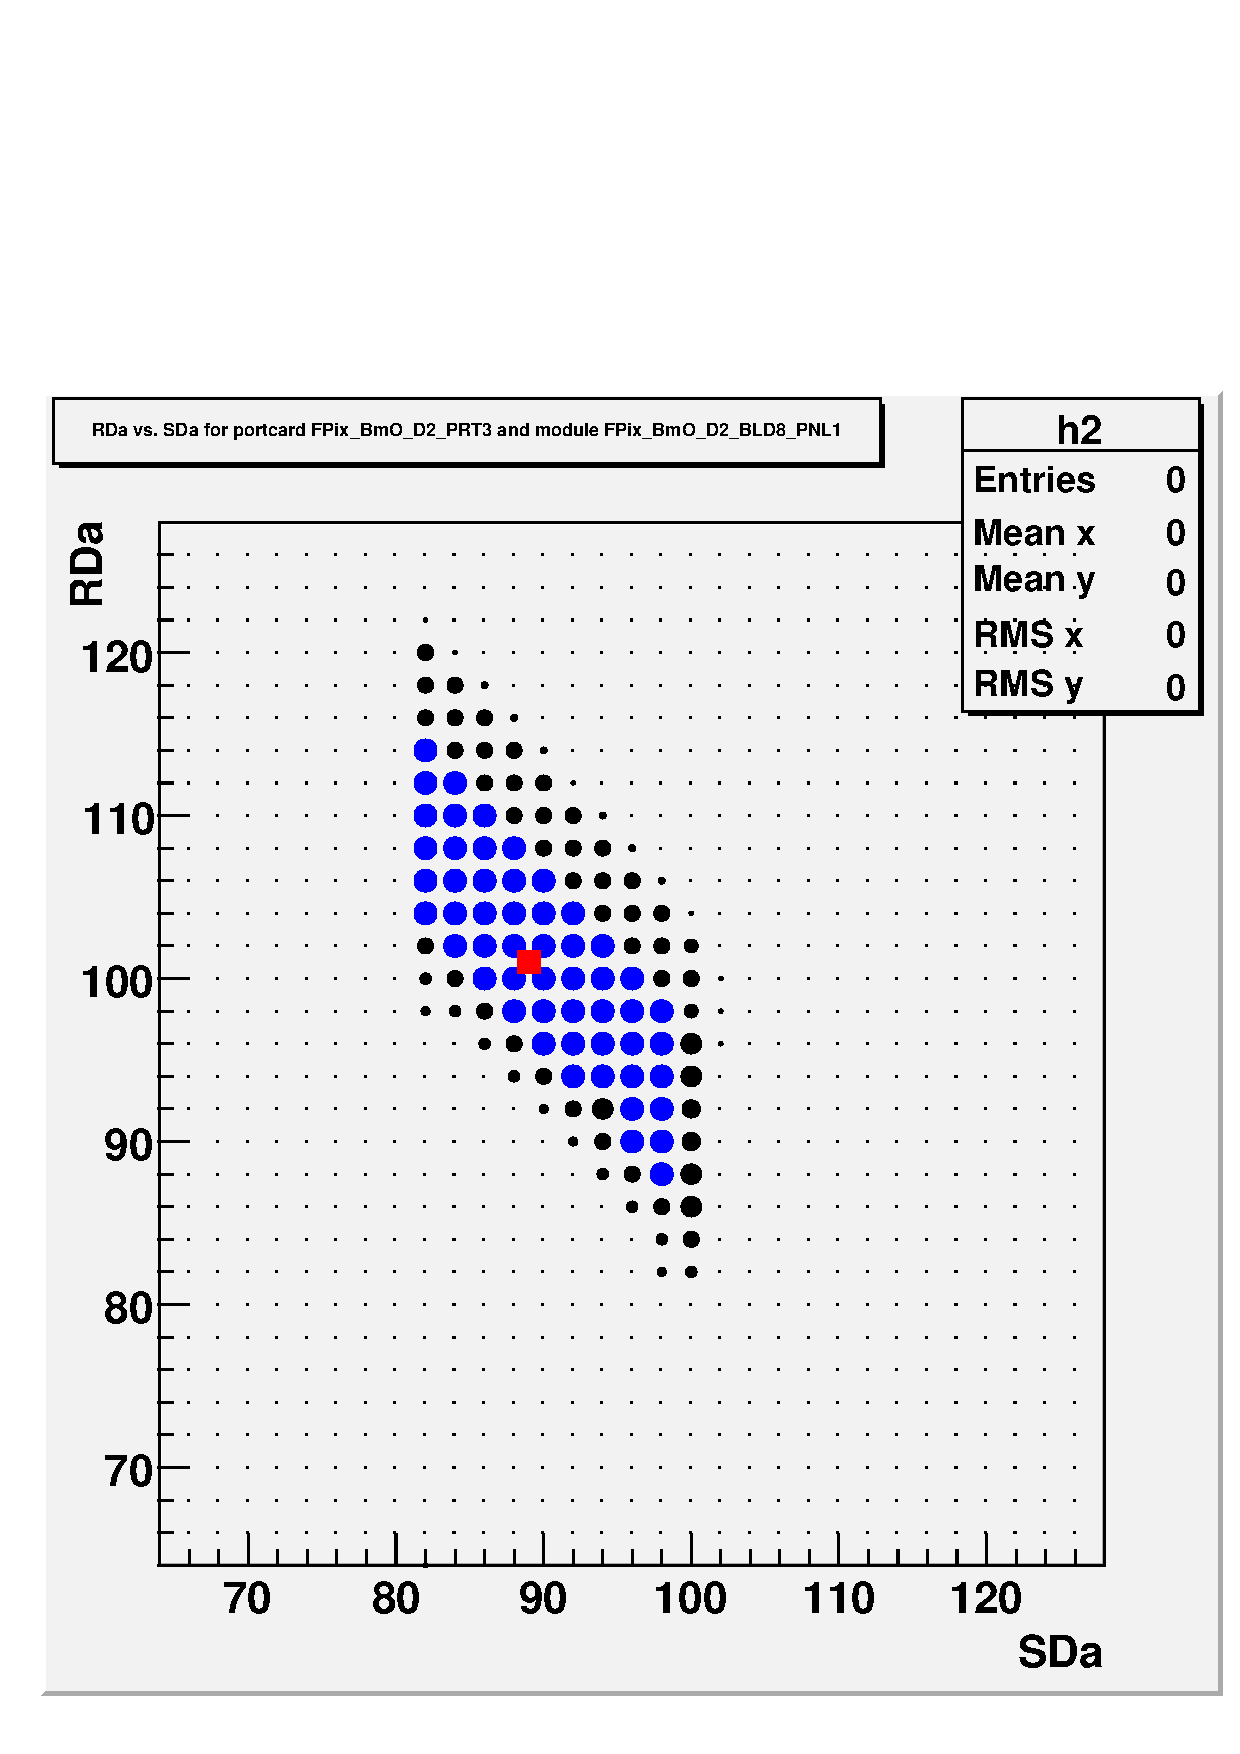
\includegraphics[width=0.8\textwidth]{graph_FPix_BmO_D2_PRT3_FPix_BmO_D2_BLD8_PNL1.pdf}
\end{center}
\caption{
This plot shows efficiency as a function of RDa and SDa. The blue
dots indicates areas with 100\% transmission efficiency. The black
dots indicated partial efficiency, larger dots have higher efficiency.
The red square indicates the point chosen by the algorithm.
}
\label{fig:Delay25Scan}
\end{figure}

\begin{figure}
\begin{center}
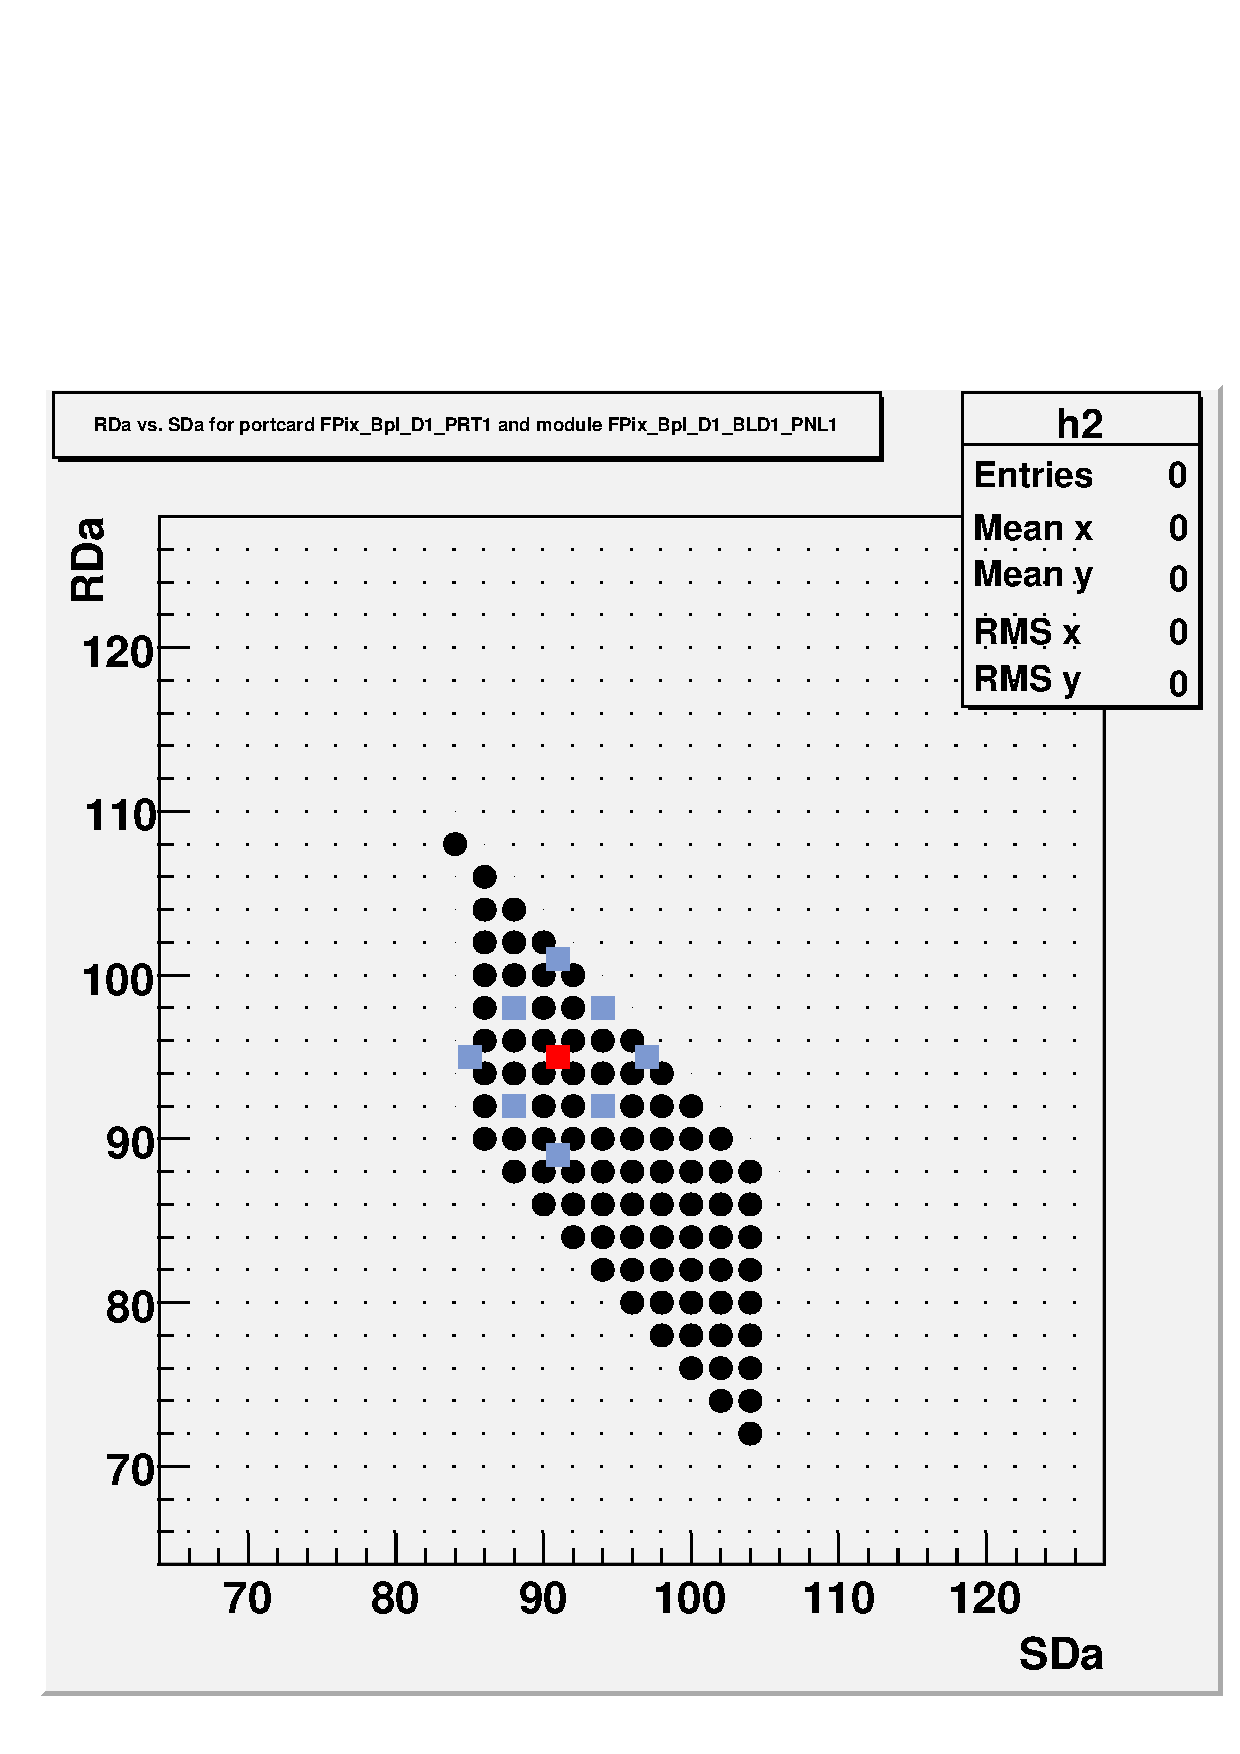
\includegraphics[width=0.48\linewidth]{graph_FPix_BpI_D1_PRT1_FPix_BpI_D1_BLD1_PNL1_0}
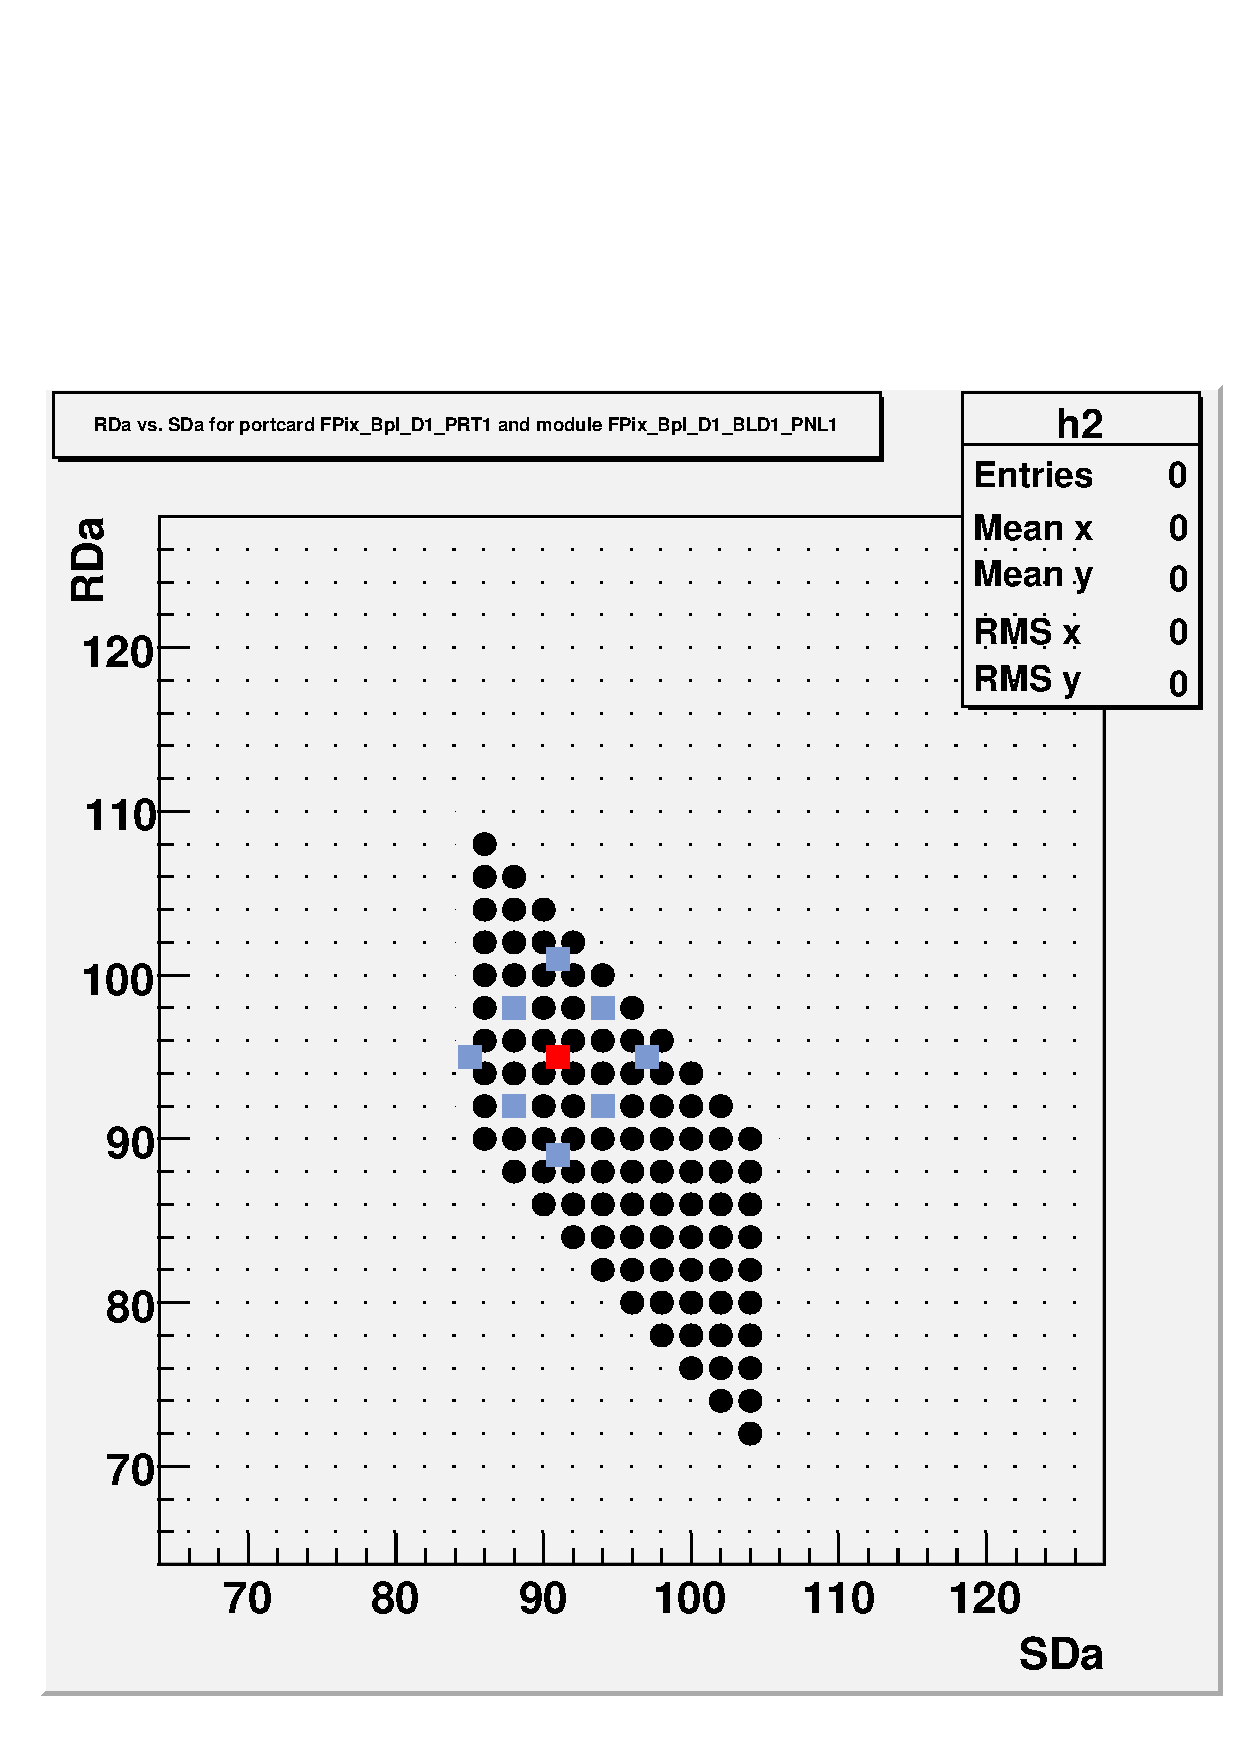
\includegraphics[width=0.48\linewidth]{graph_FPix_BpI_D1_PRT1_FPix_BpI_D1_BLD1_PNL1_1}
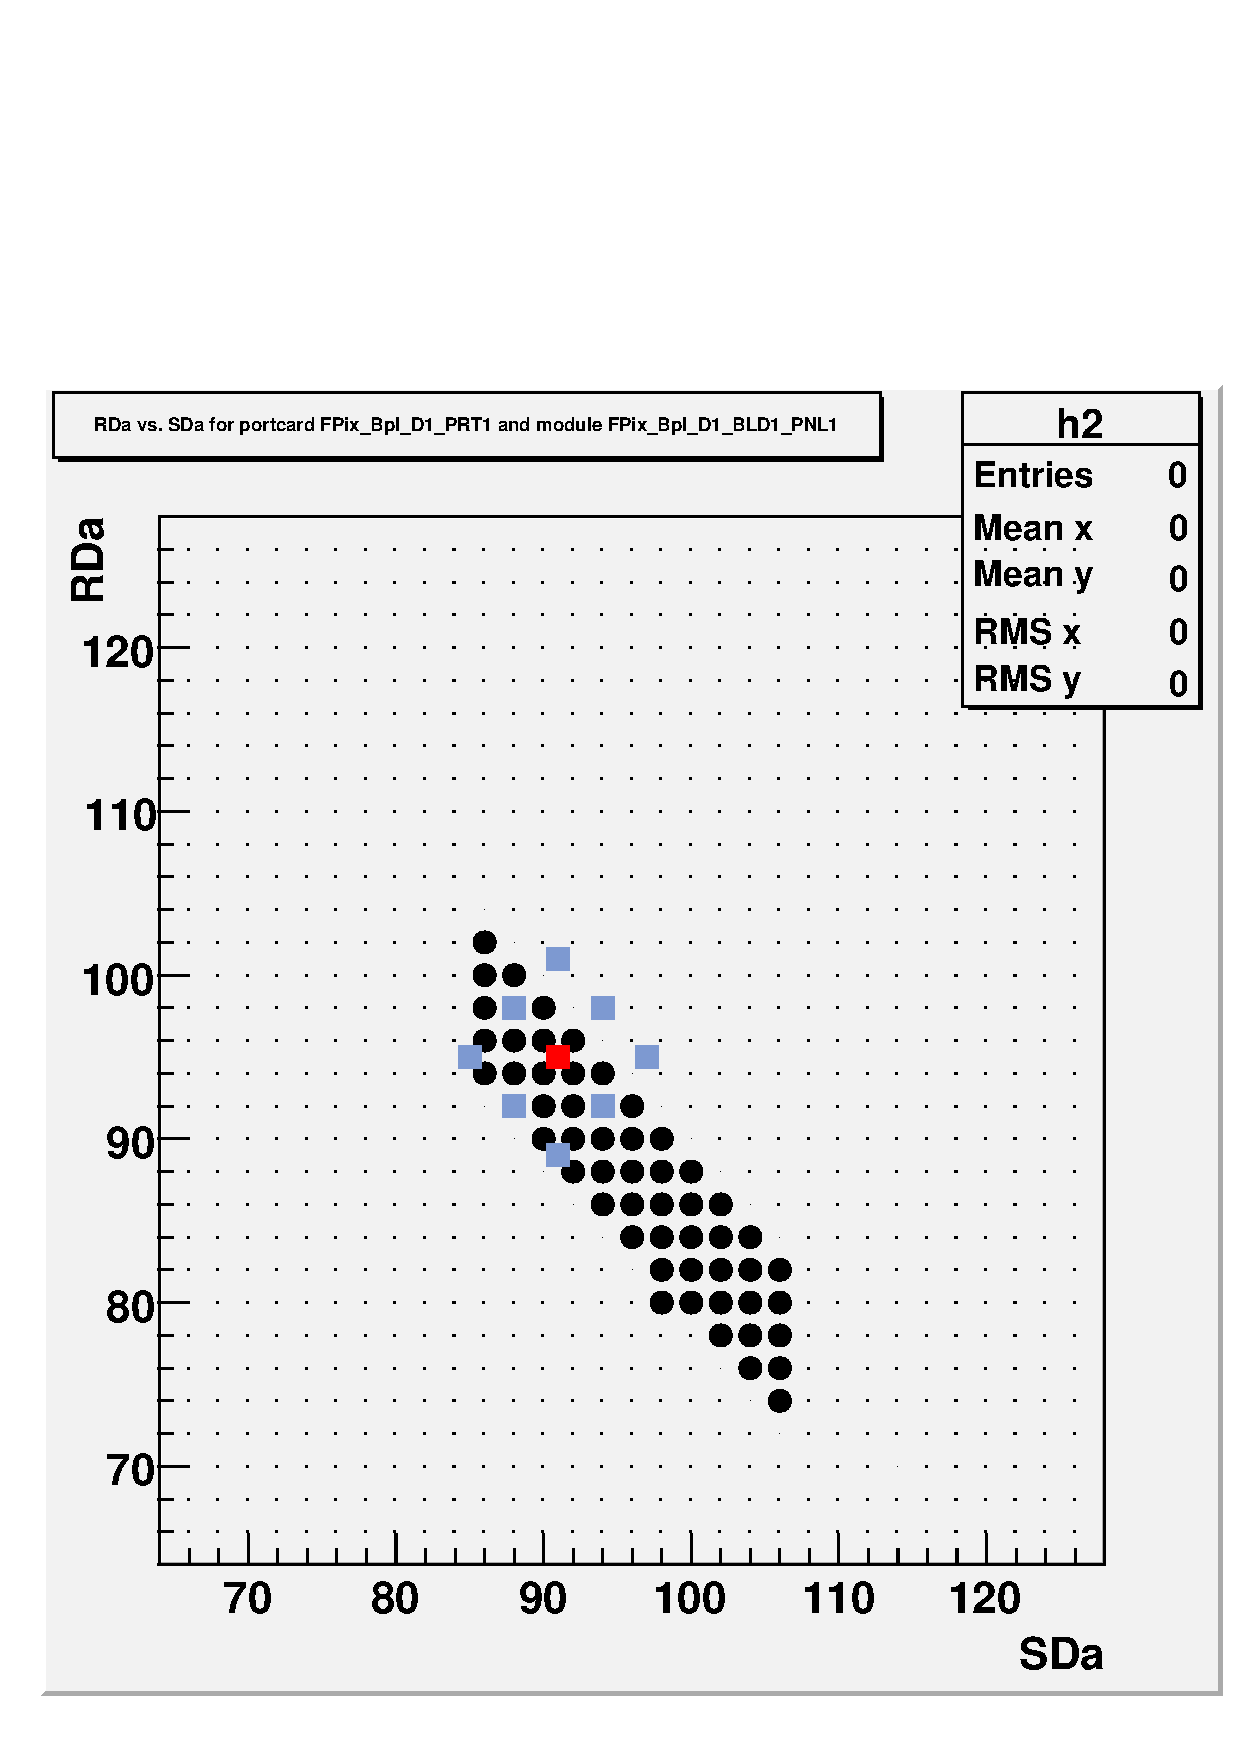
\includegraphics[width=0.48\linewidth]{graph_FPix_BpI_D1_PRT1_FPix_BpI_D1_BLD1_PNL1_2}
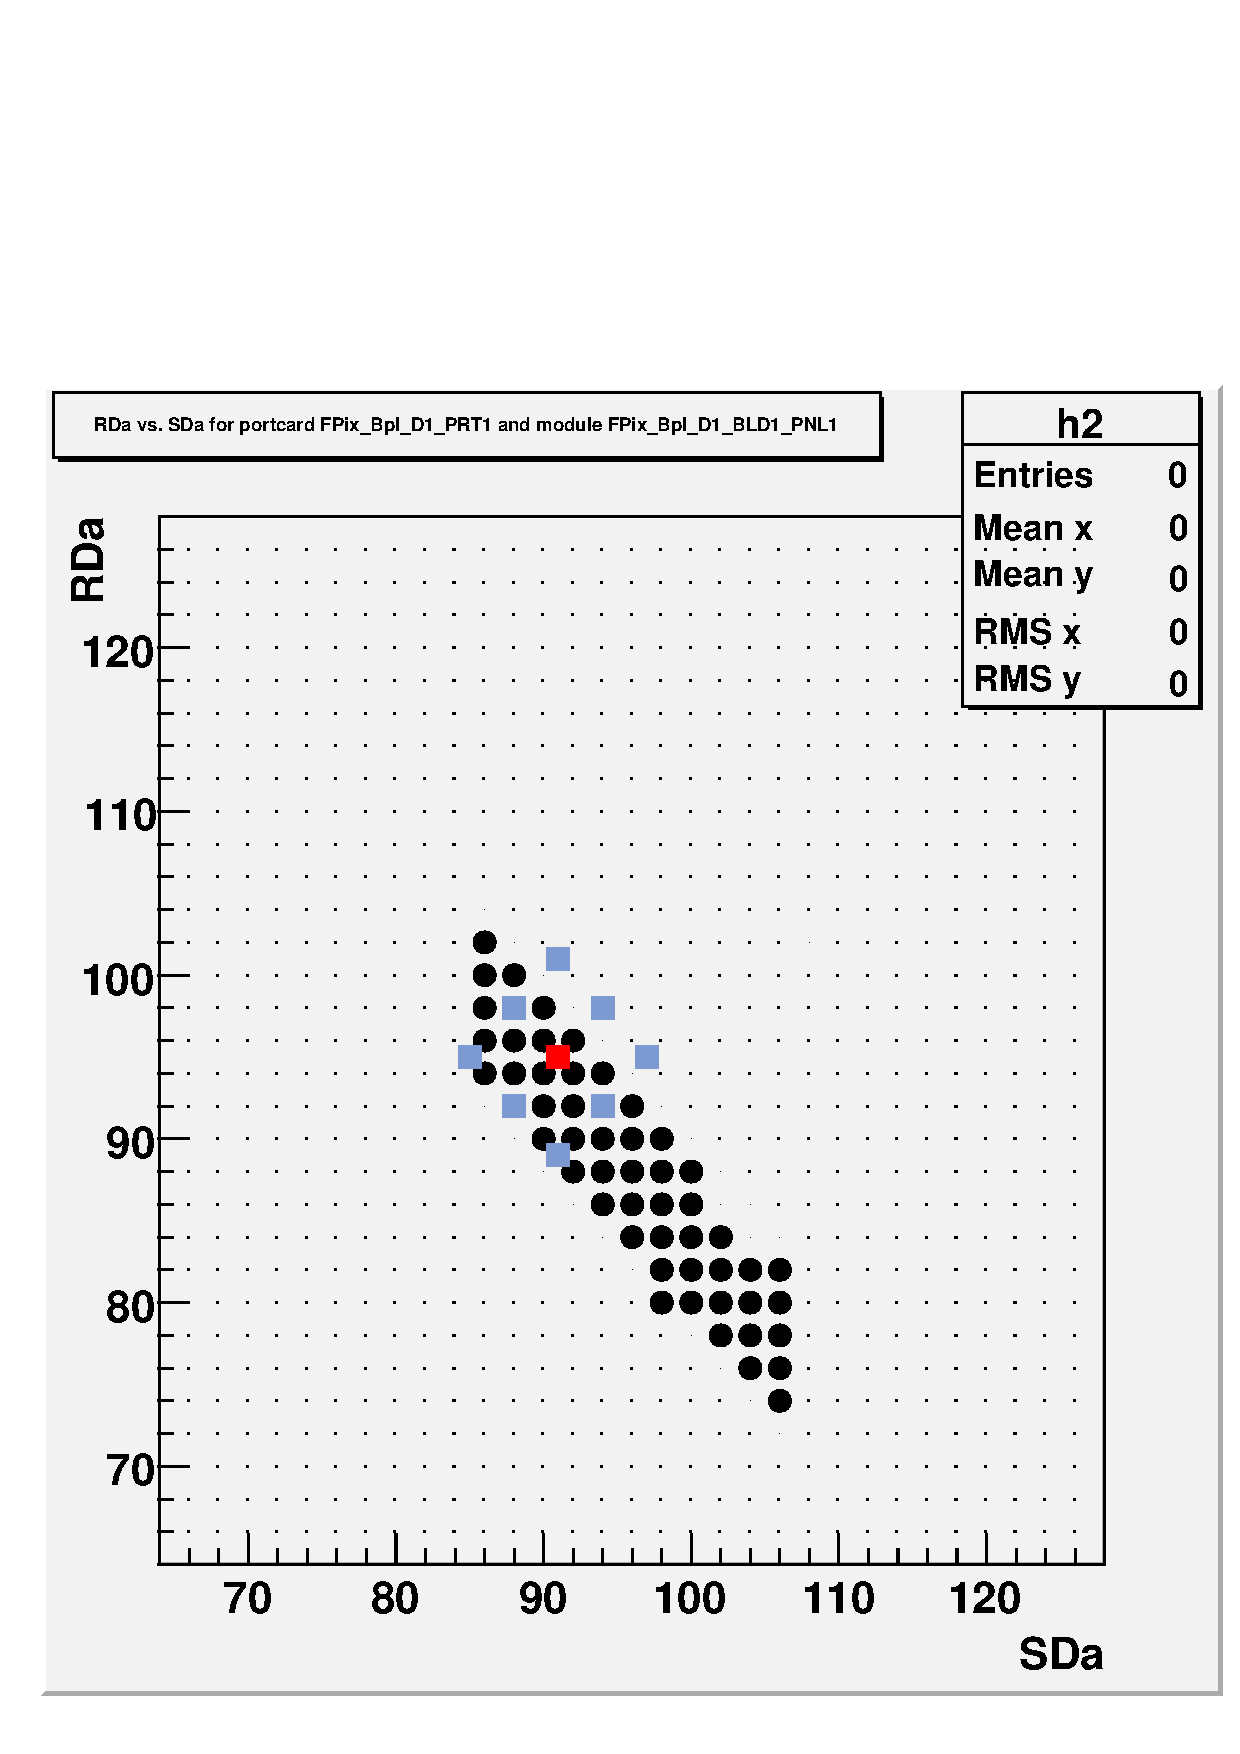
\includegraphics[width=0.48\linewidth]{graph_FPix_BpI_D1_PRT1_FPix_BpI_D1_BLD1_PNL1_3}
\end{center}
\caption{This figure shows the results of scans for delay25 settings on
the Cornell test stand. The upper left plots shows (large black dots) the
region for which the return data was valid when sending a ROC command (CalPix).
The upper right plot shows the valid region when sending a TBM command
(tbm speed). The lower left shows the region of success when sending a
roc init and the lower right shows the region of success with a roc trim
load command. As is seen, the working region is smaller for the long
commands. The red and blue points indicates the algorithm used to select
the operating point.}
\label{fig:scanDelay25}
\end{figure}



\subsection{Delay25 trigger setting}

Scans the trigger delay to
make sure that the triggers are received correctly. The delay
setting is scanned and the corresponding FED channel is read
to make sure the trigger has arrived. This has to be done
before the phase and delay scan of the FED.


\subsection{FED baseline calibration}

This calibration adjusts the input offset and channel
offsets of the optical receivers in the FED such that the
black level is adjusted to be near a given target value,
normally 450, which is near the midpoint of the
dynamic range of the ADC. During this calibration the
baseline correction in the FED is turned off.

Besides determining the input offset and the channel
offsets the algorithm determines address levels for the
black and ultra-black levels.

% Souvik


\subsection{AOH bias settings}

\subsubsection{Introduction and discussion}
The AOH bias is a setting on the port card which controls the
amount of light sent to the FED.  There is one AOH bias setting
per FED channel.  As AOH bias increases, more light is sent,
and the ADC values on the FED increase.  At low values of AOH
bias, both black and ultrablack do not change with AOH bias,
and there is no separation between black and ultrablack levels.
At some threshold, the black level begins to increase
approximately linearly.  At a higher threshold, the ultrablack
level also starts to increase linearly with approximately the
same slope.  This behavior is illustrated in
Fig.~\ref{fig:AOHBiasScan}.

\begin{figure}
\begin{center}
 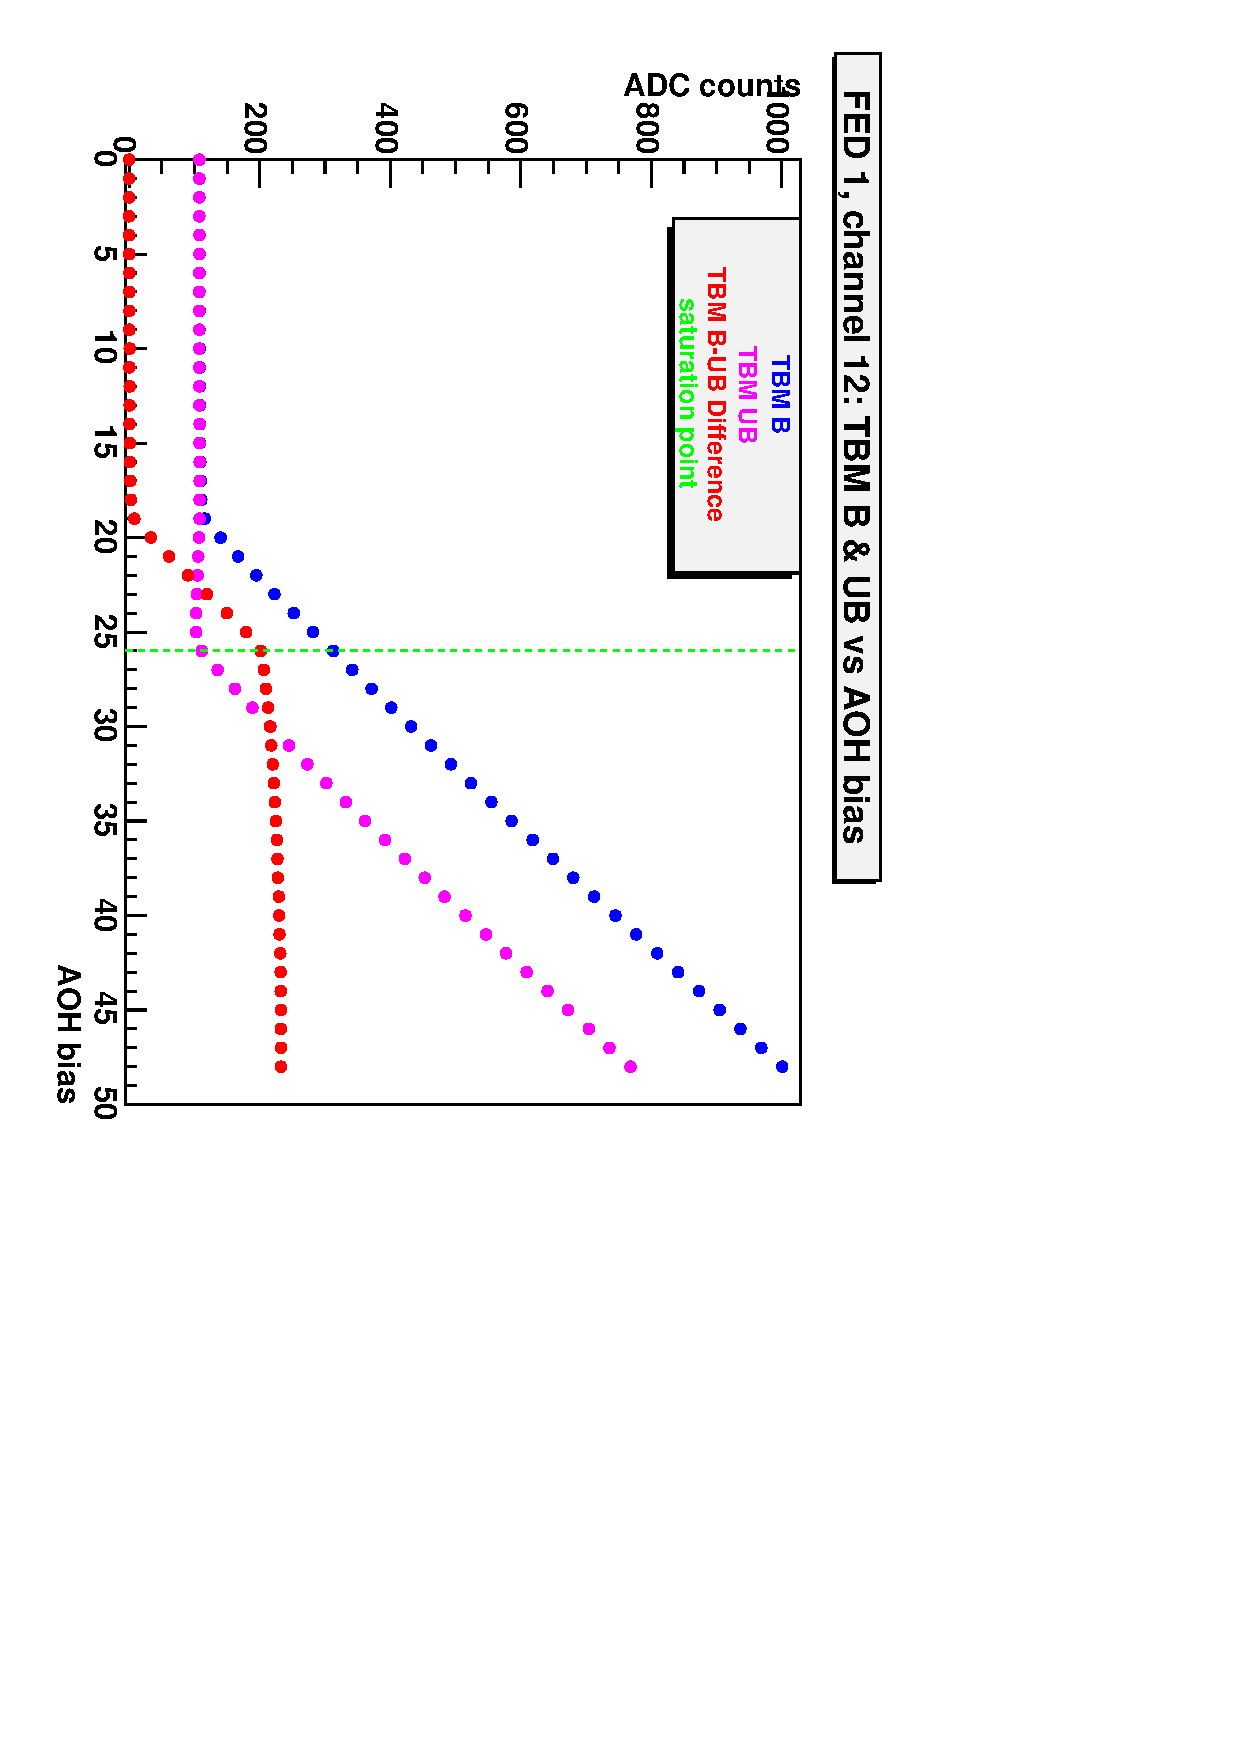
\includegraphics[angle=90,width=0.99\textwidth]{AOHBiasScan.pdf}
\end{center}
\caption{Black and ultrablack levels as a function of AOH bias.}
\label{fig:AOHBiasScan}
\end{figure}

Note that the maximum black-ultrablack separation depends on how
the TBM DACs are set.  At low DAC settings, the TBM outputs a
signal with relatively low separation; as these settings increase,
the separation also increases.  In the AOH bias scan, the black
level is independent of the TBM settings.  However, the linear
rise of the ultrablack level begins at a later point for higher
TBM settings, and hence the black-ultrablack difference saturates
at a higher AOH bias value when the TBM DAC settings are higher.

The goal of the AOH bias calibration is to determine an AOH bias
setting for each channel that is just high enough to saturate the
black-ultrablack difference.  The calibration measures this
difference, using black and ultrablack levels from the TBM header
and trailer, as a function of AOH bias.  It is important, though,
that during the scan the TBM DACs are set at least as high as they
will be set in later calibrations and physics runs.  Otherwise, the
AOH bias value determined from the saturation point will be too low.
TBM settings above those used in this scan will not increase the
B-UB separation because the AOH cannot provide more separation.

Temperature variations alter the response of the AOH, essentially shifting the curves in Figure \ref{fig:AOHBiasScan} to the left or right.  In order to provide a margin of error for temperature changes, the AOH bias should be set higher than the saturation value.  A temperature increase of 5 degrees Celcius will shift the curves by about 4 AOH bias counts.  Therefore, by default the chosen AOH bias setting will be 4 counts higher than the saturation value.  This offset is a configurable parameter.

It is also important that the AOH bias not be too high; otherwise
the FED offsets could not bring the signal into the dynamic range
of the FED.

The last part of the AOH bias calibration is to do a coarse baseline
adjustment.  The FED channel offsets are set to the center of the
range (127), and then the FED optical receiver offsets and AOH bias settings
are adjusted to bring all FED baselines into a wide target range.  AOH bias
is not decreased below the saturation value unless it is absolutely necessary.
The end result is a configuration of AOH bias and FED offset values that puts
all FED baselines near the center of the dynamic range, with AOH bias values
that allow for a large B-UB separation.  After the AOH bias calibration, the
FED baseline calibration should be run to perform fine adjustments of the
baseline (using the freedom to move each channel offset).

\subsubsection{AOH bias calibration steps}
This calibration involves many distinct steps.  They are listed in order
below.  Each step is performed on each channel being calibrated.
\begin{enumerate}
\item Set the FED channels to the 2V peak-to-peak range in order to provide
maximum dynamic range for the AOH bias scan.
\item Turn off the FED automatic baseline correction.
\item Issue \verb|ClrCal| to all ROCs, and disable hits with the control
register on all ROCs, to ensure that no hits are output.
\item Set all TBM DACs to high values.  These values may be specified as
parameters in \verb|calib.dat|.
\item Set all FED optical receiver input offsets to the highest useful value
(the setting that minimizes the FED ADC values, without impairing the B-UB
separation).  This value is configurable, and it defaults to 8 (on a scale
from 0 to 15).  Also, all channel offsets are set their maximum value, 255.
\label{item:FEDReceiverOffset}
\item Issue \verb|LRES| and \verb|CLRES| commands to all FEDs to clear the
transparent data.  This ensures that no stale data is sitting in the buffer.
\item Loop over AOH bias values.  Attempt to decode the transparent
buffer on each trigger, assuming the correct number of ROCs and no hits.
That is, find the TBM header, and verify that the TBM trailer is in the
right place.  When decoding is successful, record the start slot of
the TBM header and trailer.  On each channel, this slot should be the same for
all triggers.  The reason for this step is to find the time slots for later
use in reading out TBM B and UB levels, even at low AOH bias settings where
full decoding would fail.  If no reliable time slots are found\footnote{A time slot is considered found if the most common start slot occurs on at least 95\% of the triggers.  Alternatively, if the two most frequent time slots differ by 1 (due to a jumping clock) and together account for at least 95\% of triggers, then the time slots are considered found, and TBM B and UB are sampled only in those time slots which are known to be B or UB for either of the two start slots.} on a channel,
this channel is considered failed, and it is ignored in the rest of the
routine.
\item Now scan over AOH bias again, this time to record the TBM B and UB
levels at each setting, using the time slots recorded in the previous step\footnote{If good time slots were not found on a given channel, only the black level will be recorded and plotted.  It is taken from the first 10 slots of the transparent buffer, rather than from the TBM header and trailer.  This plot is for diagnostic purposes only; it is not used in generating new configuration settings.}.
During the
scan, if the signal goes out of range high or low, the FED channel offset is adjusted to bring it back into
range, if possible.  Since only the B-UB difference is of interest, coherent
shifts in B and UB do not matter.  The FED optical receiver offset is not adjusted during the scan -- it remains at the high setting described in step \ref{item:FEDReceiverOffset}.
\item Output plots of the TBM black and ultrablack, and the difference, as a
function of AOH bias, to a ROOT file.  Figure~\ref{fig:AOHBiasScan} is an example of the
plots produced.  Find the AOH bias value at which the B-UB difference
saturates (defined as a reduction in the slope to less than 20\% of its
maximum value).  Set each AOH to its saturation value plus the offset defined by the parameter \verb|SaturationPointOffset| (which defaults to 4).
\item Set FED channels back to the 1V peak-to-peak range, for those channels
which were originally set at 1V in the FED configuration file.  This is done
so that the coarse baseline adjustment will be done with the range that will
be used for future data-taking.
\item Set FED optical receiver input offsets to 0 (lowest value,
corresponding to highest FED ADC values), and all channel offsets to 127
(middle of the range).  The channel offset will be left at 127 for the rest
of the routine.
\item Measure black levels on all channels.  On each FED optical receiver,
if any channel has a black level above the target range, increase that
receiver's offset by one.  If not, do nothing.  Repeat this until all
channels have black levels in or below the target range, or have a receiver
offset equal to the maximum value described in
step \ref{item:FEDReceiverOffset} (defaults to 8).  The idea here is to
ensure that no AOH bias value will have to be decreased to place the black
level in the target range (unless this is absolutely necessary because the
receiver offset cannot be increased further).
\item Again measure the black levels on all channels.  If a channel's black
level is within the target range, that channel is done.  If it is above or
below the target range, decrease or increase AOH bias.  Repeat this until all
channels are within range.  (Or, if two adjacent AOH bias values produce
black levels that straddle the target range, choose the one that is closer to
the target.)  AOH bias should not have to decrease unless the FED receiver
input offset was at maximum.  If it does decrease, a warning is generated in
the summary at the end of the calibration.
\item Turn FED automatic baseline correction back on.
\item Write new config files for all port cards and FEDs with at least one
successfully calibrated channel.
\item Print a summary to the screen.  Thus summary gives the number of
successful and failed channels, statistics on the new settings for successful
channels, descriptions of the errors on unsuccessful channels, and warnings
for channels on which the final AOH bias setting is below the saturation
point.
\end{enumerate}

\subsubsection{Parameters}
A number of parameters in \verb|calib.dat| may be used to control the
calibration.

Only two ``standard" parameters are used.  The ``\verb|Repeat:|" parameter
determines the number of triggers in each step (at each AOH bias scan point
and when measuring black levels in the coarse baseline adjustment).  The
channel list is used to determine which channels are calibrated.  Note that
the rows, columns, and DAC scan settings in \verb|calib.dat| are completely
ignored.

Many other optional parameters may be set.  All have default values which
will be used if the parameter is not set.  These parameters, their defaults,
and their functionality are given in Table~\ref{tab:AOHBiasParameters}.

\begin{table}
\centering
\caption{Optional parameters for AOH bias calibration.}
\label{tab:AOHBiasParameters}
\begin{tabular}{l@{~~~~}r@{~~~~}l}
\hline
\hline
Parameter & Default & Description \\
\hline
ScanMin                     &   0 & Low end of AOH bias scan range \\
ScanMax                     &  50 & High end of AOH bias scan range \\
ScanStepSize                &   1 & Step size for AOH bias scan \\
TargetBMin                  & 412 & Allowed range for the coarse baseline \\
TargetBMax                  & 612 & adjustment at the end of this calibration \\
SaturationPointOffset       &   4 & After finding the saturation point, this \\
                            &     & number is added to get the AOH bias setting \\
                            &     & (but before adjusting the black level). \\
MaxFEDReceiverInputOffset   &   8 & Largest allowed value of the FED receiver \\
                            &     & input offset, which can range from 0 to 15 \\
SetAnalogInputBias          & 200 & TBM settings to use \\
SetAnalogOutputBias         & 120 & for all channels -- \\
SetAnalogOutputGain         & 200 & all 3 should be set high \\
printFEDRawData             &  no & Whether to print decoded transparent buffer \\
printFEDOffsetAdjustments   &  no & Whether to print when the FED offsets change \\
printAOHBiasAdjustments     &  no & Whether to print a message when the AOHBias \\
                            &     & is changed during the baseline adjustment \\
\hline
\hline
\end{tabular}
\end{table}

\subsection{AOH gain calibration}

\subsubsection{Introduction and discussion}

The AOH gain is a setting for each optical link (from detector to FED) that has just 4 possible settings (0, 1, 2, 3).  This setting does not change the black level.  Instead, it scales the size of deviations from the black level, expanding or shrinking the signal.  Larger settings correspond to larger deviations.  In particular, the separation between black and ultrablack levels will be larger at a larger gain.  Settings on the TBMs and ROCs will be the primary means of adjusting the ultrablack to the desired level, but the AOH gain must be set large enough in order to make possible a low enough ultrablack.  However, AOH gain should not be set too high since larger settings will increase the power drawn, and larger settings are intended to be used to compensate for radiation damage over time.

The aim of this calibration is to set the AOH gain at the lowest level that will allow the TBM UB level to be low enough.  The three TBM DACs (described in Sec.~\ref{sec:TBMUB}) are set to high values.  Then, for each FED channel, TBM UB is recorded as a function of AOH gain.  To choose an AOH gain setting, the calibration selects the smallest value that produces an UB below a user-defined threshold.

\subsubsection{AOH gain calibration steps}

The calibration consists of the following steps:
\begin{enumerate}
\item Issue \verb|ClrCal| to all ROCs, and disable hits with the control
register on all ROCs, to ensure that no hits are output.
\item Issue \verb|LRES| and \verb|CLRES| commands to all FEDs to clear the
transparent data.  This ensures that no stale data is sitting in the buffer.
\item Set all TBMs to high values.  The user may specify these values; otherwise defaults will be used.
\item Scan over values of AOH gain.  Attempt to decode the transparent
buffer on each trigger, assuming the correct number of ROCs and no hits.
That is, find the TBM header, and verify that the TBM trailer is in the
right place.  If decoding is successful, record the
UB values in the TBM header and trailer (5 values per trigger, 3 from the
header and 2 from the trailer).  If decoding is unsuccessful, ignore that
trigger, and don't record anything.  For each channel, a plot of this scan is
output to a ROOT file.
\item Analyze the recorded scan data on each FED channel, looking for the
smallest AOH gain where the UB is below the threshold specified by the user.  This is the recommended AOH gain value.  (If all values were above the threshold, set the AOH gain to 3 and generate an error.)
\item On dual TBMs, check whether we can reduce the difference in UB levels by raising one of the two AOH gains by 1.  If so, do it.  This minimizes the spread between ultrablack levels on dual TBMs.  (Since the two channels share the same TBM DAC settings, there is no other way to independently adjust the TBM UB levels.)
\item Write out new port card configuration files with the new AOH gain settings.
\item Print out a summary.
\end{enumerate}

\subsubsection{Parameters}
A number of parameters in \verb|calib.dat| may be used to control the
calibration.

Only two ``standard" parameters are used.  The ``\verb|Repeat:|" parameter
determines the number of triggers in each step of the scan.  The channel list
is used to determine which channels are calibrated.  Note that the rows,
columns, and DAC scan settings in \verb|calib.dat| are completely ignored.

Many other optional parameters may be set.  All have default values which
will be used if the parameter is not set.  These parameters, their defaults,
and their functionality are given in Table~\ref{tab:AOHGainParameters}.

\begin{table}
\centering
\caption{Optional parameters for AOH gain calibration.}
\label{tab:AOHGainParameters}
\begin{tabular}{l@{~~~~}l@{~~~~}l}
\hline
\hline
Parameter & Default & Description \\
\hline
SetAnalogInputBias   & 160                & Value of AnalogInputBias to set on all channels. \\
SetAnalogOutputBias  & 110                & Value of AnalogOutputBias to set on all channels. \\
SetAnalogOutputGain  & 240                & Value of AnalogOutputGain to set on all channels. \\
MaxTBMUB             & 100                & TBM UB threshold.  AOH gain will be set so \\
                     &                    & that TBM UB is below this level. \\
printFEDRawData      & no                 & Whether to print decoded transparent buffer \\
printScan            & no                 & Whether to print TBM UB levels \\
                     &                    & for each AOH gain \\
\hline
\hline
\end{tabular}
\end{table}


\subsection{TBM UB calibration} \label{sec:TBMUB}

\subsubsection{Introduction and discussion}

With the black level set at 512 by the baseline calibration and automatic
baseline correction, the next step is to set the ultrablack levels
appropriately.  We first adjust DACs on the TBM to set the TBM header and
trailer ultrablack to an appropriate value. (Experience
from forward testing suggests that a value of 120 to 150 is good.)

There are three DAC settings on the TBM, all of which affect the ultrablack
level.  Higher values of these DACs correspond to lower ultrablack (and
greater B-UB separation).  Figure~\ref{fig:tbm-anal-dacs} shows how these
DACs affect the output of the TBM.  The \verb|AnalogOutputGain| setting
alters the levels of the TBM header and trailer, but not the signals from
the ROCs.  The \verb|AnalogInputBias| setting affects both ROC and TBM
signals, but it changes ROC signals more than TBM signals.  The
\verb|AnalogOutputBias| setting affects ROC and TBM signals equally.
The TBM UB level may be adjusted by any or all of these three DAC settings.

\begin{figure}
\begin{center}
 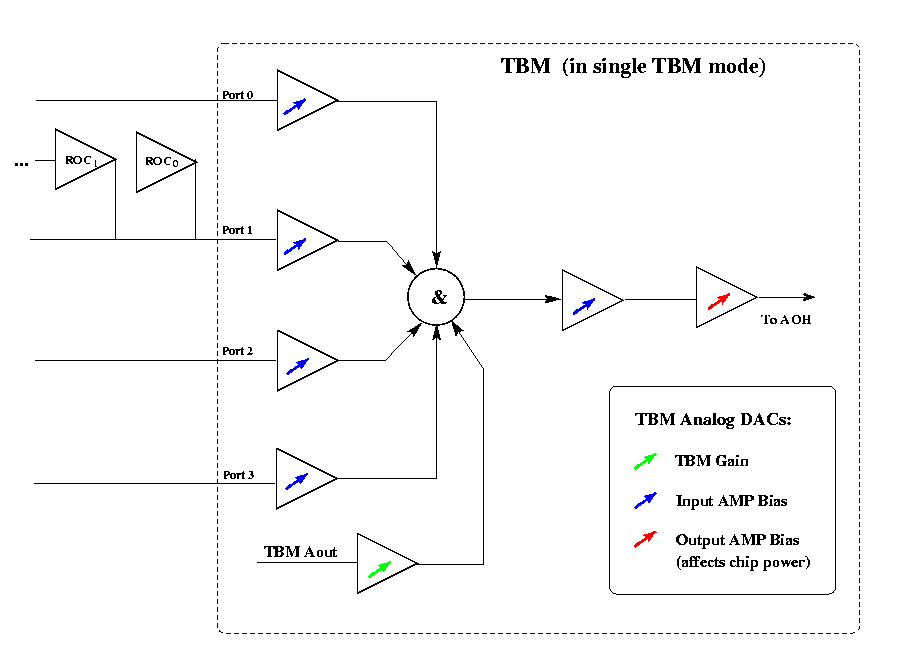
\includegraphics[width=0.99\textwidth]{tbm-anal-dacs.png}
\end{center}
\caption{Diagram illustrating how the TBM DACs affect the output of the TBM.
AnalogInputBias is referred to as Input AMP Bias (blue arrows),
AnalogOutputBias is referred to as Output AMP Bias (red arrows),
and AnalogOutputGain is referred to as TBM Gain (green arrows).}
\label{fig:tbm-anal-dacs}
\end{figure}

Although higher DAC values generally produce lower ultrablack levels, at very high DAC values the ultrablack level may actually increase.  In particular, \verb|AnalogOutputBias| should not exceed $\sim$128.  If the calibration finds multiple settings that give the target ultrablack level, it will choose the lower settings.

The TBM UB calibration routine can run in either of two modes, as selected by the user:
\begin{enumerate}
\item Fix two DAC settings and scan the third.  The user selects which DAC to scan and specifies the scan range.  Optionally, the other two DACs may be given particular settings for all ROCs; otherwise the values stored in the configuration database will be used.
\item Scan all three settings simultaneously.  The user selects a scan range for each DAC, as well as the number of scan points.  During the scan, all three settings are moved simultaneously and proportionally through their ranges.  Specifically, for scan point $i = \{0, 1,..., N-1\}$, the value of DAC $d$ is
\begin{equation}
v_{d}(i) = min_{d} + \frac{i}{N-1} \times (max_{d}-min_{d})
\end{equation}
where $N$ is the number of scan points and $min_{d}$ and $max_{d}$ are the minimum and maximum scan values for DAC $d$.
\end{enumerate}
In either mode, the calibration
searches for DAC settings that put the TBM UB at the target level.
(This level defaults to 135, and may be changed by the user.)  The second mode, where all three settings are varied simultaneously, is recommended.

Dual TBMs are a special case.  The two channels on a dual TBM share the
same DAC settings, so they cannot be adjusted independently.  Therefore the
TBM settings cannot be adjusted to simultaneously put both channels' UB at
the target level.  For dual TBMs, we set the DACs so that one channel is at
the target UB level, and the other is below.

\subsubsection{TBM UB calibration steps}

The calibration consists of the following steps:
\begin{enumerate}
\item Issue \verb|ClrCal| to all ROCs, and disable hits with the control
register on all ROCs, to ensure that no hits are output.
\item Issue \verb|LRES| and \verb|CLRES| commands to all FEDs to clear the
transparent data.  This ensures that no stale data is sitting in the buffer.
\item Scan over DAC values as specified by the user, either varying just one DAC or varying all three simultaneously.  Attempt to decode the transparent
buffer on each trigger, assuming the correct number of ROCs and no hits.
That is, find the TBM header, and verify that the TBM trailer is in the
right place.  If decoding is successful, record the
UB values in the TBM header and trailer (5 values per trigger, 3 from the
header and 2 from the trailer).  If decoding is unsuccessful, ignore that
trigger, and don't record anything.  For each FED channel, a plot of this scan is
output to a ROOT file.
\item Analyze the recorded scan data on each FED channel, looking for the
point where the measured UB crosses the target level.  When the crossing is
found, interpolate between the nearest scan points for the best DAC settings.
If no crossing is detected, the channel
is considered failed.  If multiple crossings are detected, a warning is generated for that channel.  New DAC settings will still be generated if the scan contains some data -- either the value that puts the UB closest to the target, or the leftmost crossing point (lowest DAC values) if there are more than one.
\item On single TBMs, the new DAC values are the values at this crossing point.
On dual TBMs, the new DAC values are the higher of the two sets of values found on the
two FED channels for that TBM; this ensures that both UB levels will be at or
below the target.  If only one of the two channels was on the list of channels to calibrate, then the new DAC value is based on the one channel, and a warning is generated.  A warning is also generated if both channels were successful, but the DAC values were too far apart.
\item Write out new TBM configuration files for the
modules with new DAC settings (including any settings which were not varied during the scan).
\item Print out a summary.
\end{enumerate}

\subsubsection{Parameters}
A number of parameters in \verb|calib.dat| may be used to control the
calibration.

Only two ``standard" parameters are used.  The ``\verb|Repeat:|" parameter
determines the number of triggers in each step of the scan.  The channel list
is used to determine which channels are calibrated.  Note that the rows,
columns, and DAC scan settings in \verb|calib.dat| are completely ignored.

One other parameter is required.  The parameter \verb|DACToScan| must be set to \verb|AnalogInputBias|, \verb|AnalogOutputBias|, \verb|AnalogOutputGain|, or \verb|All|.  Selecting \verb|All| will scan all three DACs simultaneously; otherwise just one is scanned.

Many other optional parameters may be set.  All have default values which
will be used if the parameter is not set.  These parameters, their defaults,
and their functionality are given in Table~\ref{tab:TBMUBParameters}.

\begin{table}
\centering
\caption{Parameters for TBM UB calibration.  All except DACToScan are optional.}
\label{tab:TBMUBParameters}
\begin{tabular}{l@{~~~~}l@{~~~~}l}
\hline
\hline
Parameter & Default & Description \\
\hline
DACToScan            & N/A                & Which of the three TBM DACs to scan, or ``All" \\
\hline
\multicolumn{3}{c}{DACToScan $\neq$ All} \\
ScanMin              & 0                  & Low end of DAC scan range \\
ScanMax              & 255                & High end of DAC scan range \\
ScanStepSize         & 5                  & Step size for DAC scan \\
SetAnalogInputBias   & [empty]            & If not set, leave AnalogInputBias unchanged. \\
                     &                    & Otherwise, set it to the specified value and\\
                     &                    & change in the output configuration file. \\
SetAnalogOutputBias  & [empty]            & If not set, leave AnalogOutputBias unchanged. \\
                     &                    & Otherwise, set it to the specified value and\\
                     &                    & change in the output configuration file. \\
SetAnalogOutputGain  & [empty]            & If not set, leave AnalogOutputGain unchanged. \\
                     &                    & Otherwise, set it to the specified value and\\
                     &                    & change in the output configuration file. \\
\hline
\multicolumn{3}{c}{DACToScan = All} \\
MinAnalogInputBias   & 0                  & Minimum AnalogInputBias value during scan \\
MaxAnalogInputBias   & 255                & Maximum AnalogInputBias value during scan \\
MinAnalogOutputBias  & 0                  & Minimum AnalogOutputBias value during scan \\
MaxAnalogOutputBias  & 128                & Maximum AnalogOutputBias value during scan \\
MinAnalogOutputGain  & 0                  & Minimum AnalogOutputGain value during scan \\
MaxAnalogOutputGain  & 255                & Maximum AnalogOutputGain value during scan \\
\hline
\multicolumn{3}{c}{Any DACToScan Setting} \\
ScanNumSteps         & 52                 & Number of scan steps -- will override \\
                     &                    & ScanStepSize setting, if present \\
TargetUB             & 135                & Desired TBM UB level \\
DualTBMMaxScanStepDiff& 6                 & If the difference in scan steps between the final DAC\\
                     &                    & settings on the two channels of a dual TBM\\
                     &                    & exceeds this value, a warning is generated. \\
printFEDRawData      & no                 & Whether to print decoded transparent buffer \\
printScan            & no                 & Whether to print TBM UB levels \\
                     &                    & for each DAC setting \\
\hline
\hline
\end{tabular}
\end{table}

\subsection{ROC UB equalization calibration}

\subsubsection{Introduction and discussion}

This calibration sets the ultrablack level for each ROC equal to the
corresponding TBM's ultrablack level.

There are two DAC settings on the ROC which affect the ultrablack level.
Higher values of these DACs correspond to lower ultrablack (and greater
B-UB separation).  \verb|VIbias_roc| affects UB, address levels, and pulse
height.  \verb|VIbias_DAC| affects UB and address levels, but not pulse
height.  In this routine, \verb|VIbias_DAC| is scanned while
\verb|VIbias_roc| is fixed.

\subsubsection{ROC UB equalization calibration steps}

This calibration is very similar to the TBM UB calibration, except that each
individual ROC is analyzed.  It consists of the following steps:
\begin{enumerate}
\item Issue \verb|LRES| and \verb|CLRES| commands to all FEDs to clear the
transparent data.  This ensures that no stale data is sitting in the buffer.
\item Scan over values of \verb|VIbias_DAC|.  (If the calib.dat file
specified a fixed value of \verb|VIbias_roc|, this is also set.)  Each time
after \verb|VIbias_DAC| is changed, issue \verb|ClrCal| to all ROCs, and
disable hits with the control
register on all ROCs, to ensure that no hits are output (so any hits
specified in the configuration file are ignored).  Attempt
to decode the transparent buffer on each trigger, assuming the correct
number of ROCs and no hits.  That is, find the TBM header, and verify that
the TBM trailer is in the right place.  If decoding is successful, record
the UB values in the TBM header and trailer, and for each ROC.  If decoding
is unsuccessful, ignore that trigger, and don't record anything.  For each
ROC, a plot of this scan is written to a ROOT file.
\item Analyze the recorded scan data on each ROC, looking for the point
where the measured ROC UB equals the UB level on the corresponding TBM.
When the ROC UB crosses the TBM UB, interpolate between the nearest scan
points for the best \verb|VIbias_DAC| setting.
If no crossing is detected, the ROC
is considered failed.  If multiple crossings are detected, a warning is generated for that ROC.  A new \verb|VIbias_DAC| setting will still be generated if the scan contains some data -- either the value that puts the ROC UB closest to the TBM UB, or the leftmost crossing point (lowest \verb|VIbias_DAC| value) if there are more than one.
\item Write out new ROC configuration files
with the new \verb|VIbias_DAC| settings.  If \verb|VIbias_roc| was
modified by the user, the output files will contain this new value, too.
\item Print out a summary.
\end{enumerate}

\subsubsection{Parameters}
A number of parameters in \verb|calib.dat| may be used to control the
calibration.

The various ``standard" parameters are used in this calibration.  The
``\verb|Repeat:|" parameter determines the number of triggers in each step
of the scan.  The ROC list is used to determine which ROCs are calibrated.

A line like
\begin{verbatim}
Scan: VIbias_DAC 80 200 5
\end{verbatim}
must be included to specify the scan range (first two numbers) and step
size (last number).

Optionally, \verb|VIbias_roc| may be set with a line like
\begin{verbatim}
Set: VIbias_roc 150
\end{verbatim}

Any hits specified in \verb|Rows:| and \verb|Columns:| will be
ignored.  (This is done by explicitly clearing them.)  The \verb|Rows:| and
\verb|Columns:| parameters should be empty; otherwise the calibration will work
but will print a warning message.

Some optional parameters may also be set.  All have default values which will
be used if the parameter is not set.  These parameters, their defaults, and
their functionality are given in Table~\ref{tab:ROCUBParameters}.

\begin{table}
\centering
\caption{Optional parameters for ROC UB equalization calibration.}
\label{tab:ROCUBParameters}
\begin{tabular}{l@{~~~~}l@{~~~~}l}
\hline
\hline
Parameter & Default & Description \\
\hline
printFEDRawData      & no                 & Whether to print decoded transparent buffer \\
printScan            & no                 & Whether to print TBM UB levels \\
                     &                    & for each DAC setting \\
\hline
\hline
\end{tabular}
\end{table}


\subsection{Address level determination}

The address level determination determines the values used
by the FED to encode the transparent data. This include
address levels for the pixel addresses, TBM header and trailer
levels, and the black and ultrablack levels.

Pixels are scanned to make sure that we probe combinations
of address levels that could potentially cause problems,
such as transitions from high to low levels and vice versa.

Due to limitations in the size of the FIFO1 transparent
data size of 512 clocks, we cannot even take one hit
per ROC unless the timing is adjusted such that the
start of the pulse train comes relatively early, i.e. in
the first 20 or so clock cycles. Recall, each ROC, with
one hit takes 9 clock cycles to read out. Then with 24 ROCs
in a module we need 216 clock cycles just to read out the
hits. Plus about 16 clock cycles to read out the TBM
headers.


\subsubsection{Data volume and time estimate}

The worst case scenario for an address level
calibration is one BPIX crate. We have 16 FED
cards in one crate, and we can assume that all
of them are fully populated. This means that we
have $16\times 36=576$ links. As we read out this
data in transparent mode we will read 1024 words
per event (even though the transparent data
is only 512 bytes long). This means a total of
235926 bytes. If we want to go thought all
pixel we have to read out 4160 times this data
volume for a total of 9,4 GB. At a speed of
10 MB/s this will take 940 s.

Assuming that we change the transparent data
FIFO to be 1024 bytes. Then we can easily
fit 4 hits into each ROC. This then cuts the
readout time by a factor of 4 as we will need
exactly 1/4 the number of triggers. This then
becomes 235 seconds.

We can also use different patterns that use
fewer pixel hits. But one has to take care to have all
relevant transitions.


\subsection{Pixel alive, Scurve, and Gain calibration}
\label{sec:PATanalysis}

The pixel alive calibration loops over pixels and injects
charge for a fixed VCal setting. The data is analyzed
to produce an efficiency map that displays the efficiency
for each pixel on a plaquette.

The Scurve and gain calibrations are variations of the
pixel alive test were we in addition loop over the VCal
setting for each pixel. For the Scurve the data is
analyzed to produce an efficiency as a function of the
VCal setting while for the gain calibration we
look at the charge (ADC value) as function of the VCal.

To analyze the data, go to PixelAnalysisTools/test and do
one of the following:
\begin{verbatim}
./bin/linux/x86/PixelAnalysis.exe PixelAlive <runnum>
./bin/linux/x86/PixelAnalysis.exe SCurve <runnum>
./bin/linux/x86/PixelAnalysis.exe Gain <runnum>
\end{verbatim}
Writing e.g. PixelAlive will pick up the default
configuration xml file, configurations/PixelAliveAnalysis.xml.
You can also specify the exact configuration file you
would like to use, e.g. configuration/PixelAliveAnalysis\_FPix.xml.

You can scan over multiple WBCs when taking this data and
analyze the data from all the WBCs summed together or only one
of them using the ChooseWBC option in the configuration xml file.
To measure absolute thresholds, use the in-time WBC and the
following one.  To measure the in-time threshold, use the
in-time WBC only.


\subsubsection{Practical issues}

If you get a lot of ``Time Out Error'' messages it could
be because you don't have the right channels enabled on the
FED. Or more specifically that you have enabled channels that
are not connected.

\subsection{Iana vs. Vana Calibration}

A calibration called ``Iana'' is implemented to
scan Vana and measure the analog current, Iana.
As the power distribution for the low voltage is
done per portcard for the forward pixels, this calibration
works in parallel on a ROC at the time on each
of the portcards. The current changes we are
measuring is of the order 50 mA as you go from
Vana=0 to Vana=255. The A4603 power module has
a resolution of about 7 mA. We perform this
measurement when all other ROCs are configured
to their default values. Hence, we measure the
current changes on top of a current of several amperes.
(I performed trials were I lowered Vana on all
other ROCs to reduce the current, but it does
not really improve the measurements.)
Hence, we have to take the data and fit it in order to
interpolate between the points. (It takes a
long time to do these measurments as one has to
wait up to 6 seconds before the current measurement
is stable.)

\begin{figure}
\begin{center}
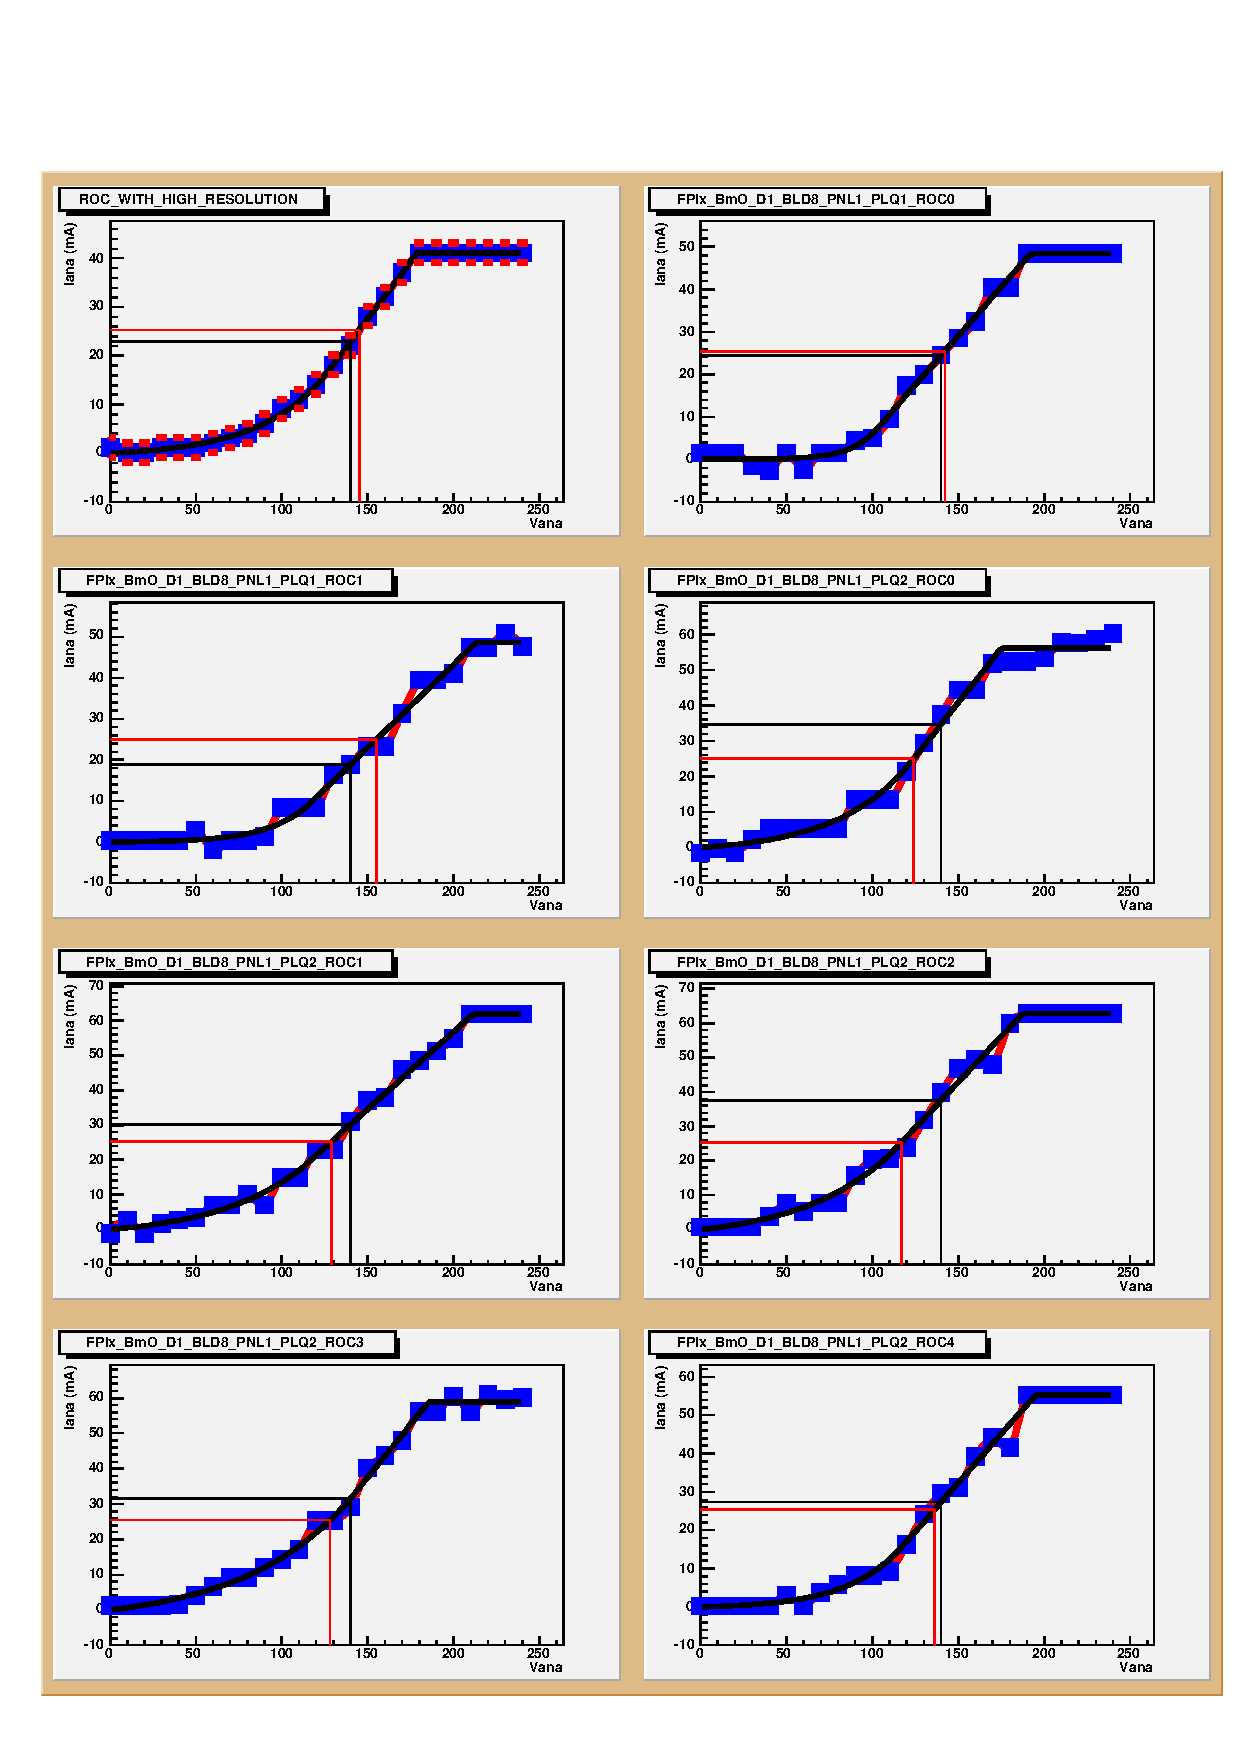
\includegraphics[width=0.85\linewidth]{IanavsVana}
\end{center}
\caption{This figure shows the measured analog current, Iana,
vs the Vana setting for a few ROCs. The top left plot shows
the Iana measured for one ROC with the A1715 power supply that
has a better resolution. The black lines indicate the default setting
(Vana=140) used in the configuration when this data was taken.
The red line indicate the setting that gives a analog current of
25 mA.}
\label{fig:IanavsVana}
\end{figure}


To analyze the data we fit it to a functional form.
After some experimentation I came up with the following.
I divide the range of Vana values into 3 ranges,
compare Fig.~\ref{fig:IanavsVana}. In the high range Iana
is taken to be a constant. In the low range Iana
is taken to be a constant plus an exponential.
In the middle range Iana depends linearly on Vana,
and the function is required to be continuous. In
addition the function is required to have a continuous
derivative as it goes between the low and middle region.
This function has 5 free parameters that are determined
in the fit.

First the raw data is fit to this form. After doing this
fit the offset at Vana=0 is subtracted and the data is
refit and plotted. These are the fits shown in Fig.~\ref{fig:IanavsVana}.

A black line is used to indicate the current for
the default Vana setting (Vana=140). In red is shown where you should
set Vana to get an analog current of 25 mA.


\subsection{Settings of CalDelay and VcThreshold}%
\label{sect:caldelvsvcthr}

These settings are ROC wide and a few pixels are selected and
a scan over the CalDelay and VcThreshold setting is performed.
For each setting, triggers are taken and data is looked at
using FIFO3 to see how many hits we had on each ROC.
In order for this algorithm to work the address levels for
black and ultra-black has to be set. (There is also an
implementation that uses the FIFO1, it does not need
address levels.)

We point out that CalDel is {\it only} relevant
for calibration data taken with charge injection.
The CalDel setting controlls the time in which the
charge is injected into the pixels. For real data
we will have to adjust the timing, e.g. using the
delay 25 settings from the trigger. However, for data
taken with charge injection this delay is important.

This calibration performs a 2-D scan of CalDel vs VcThr.
For large VcThr, which corresponds to low thresholds,
we get lots of noise and the ROC digital readout basically
shuts down and we don't see any hits. For lower
values of VcThr we get in the range of CalDel values
that corresponds to the WBC used. For larger thresholds
this curve 'bends' to lower values of CalDel. As this
curresponds to a higher threshold the signal reaches the
threshold later and hence we need to use a smaller
CalDel, i.e. inject the signal earlier.

\subsubsection{Output}

The primary output of this calibration are new
ROC DAC settings. The only settings that should be
changed in this calibration are for CalDel and VcThr.

In addition to the DAC settings the calibration produces
the output file {\tt VcThrCalDelaySummary.txt} which
lists all the ROCs that were used in the calibrations.
For each of the ROCs there is a corresponding file,
named like
{\tt ThrCalDelScan\_FPix\_BmO\_D1\_BLD8\_PNL2\_PLQ1\_ROC0.dat}.
Also, plots and a summary tree are put into a ROOT file. An example
of a plot is shown in Fig.~\ref{fig:thresholdCalDel}.

\begin{figure}[htbp]
\begin{center}
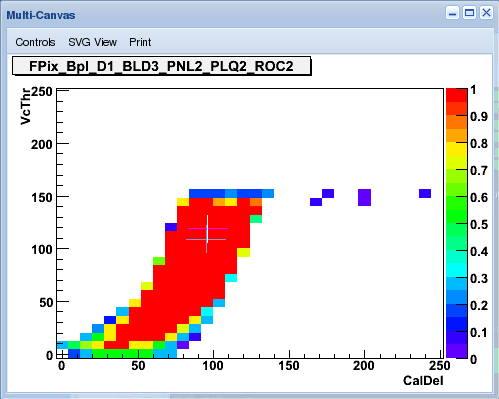
\includegraphics[width=0.8\linewidth]{VcThrCalDel_example.png}
\end{center}
\caption{The efficiency for detecting a hit is shown
as a function of VcThr vs. CalDel. Too large values
of VcThr, corresponding to a low threshold, generates
much noise that saturates the digital circuit and no
hits are seen. The optimal point is indicated in black
and the blue point indicates the old point from the
configuration.
}
\label{fig:thresholdCalDel}
\end{figure}

\subsubsection{Example}

An example configuration file is shown below.
\begin{verbatim}

Mode: ThresholdCalDelay
Rows:
10 | 20
Cols:
10 | 20
VcalHigh
Scan: VcThr 0 255 8
Scan: CalDel 0 255 8
Set: Vcal 50
Repeat: 10
ToCalibrate:
all
\end{verbatim}

\subsection{CalDel calibation}

Again the note from Sect.~\ref{sect:caldelvsvcthr} applies
in that CalDel is not relevant for physics data.

In this calibration we scan CalDel for a series
of different WBC settings. This creates a pattern
as indicated in Fig.~\ref{fig:caldel}. As
a change of one unit of WBC corresponds to
24.95ns (40.079 MHz) we can use the change in
CalDel for different WBC settings to calibrate
absolutely what a change of CalDel corresponds
to in absolute time.

We run this calibration with an injection of a large
signal (255 on the high Vcal range). We then pick
a Vcal setting that is near the {\it early} start
of the efficient range for the WBC setting. We pick
an early time so that we retain efficiency for signals
that are not as strong and takes time to get over
threshold. How close to the edge the CalDel setting
is taken can be specified by the parameter
``Fraction''. Setting this to 0 means that
you pick the point right at the early edge, setting
the parameter to 1 means that you select the late
edge.


\subsubsection{Output}

The CalDel calibration produces new ROC DAC settings
that update the CalDel settings, all other settings
should be left unchanged. The calibration also
generates output to display the region of good
efficiency in the WBC vs CalDel. The output can
be processed to generate plots using the root script
{\tt caldel.c}. An example plot is shown in
Fig.~\ref{fig:caldel}.

\begin{figure}
\begin{center}
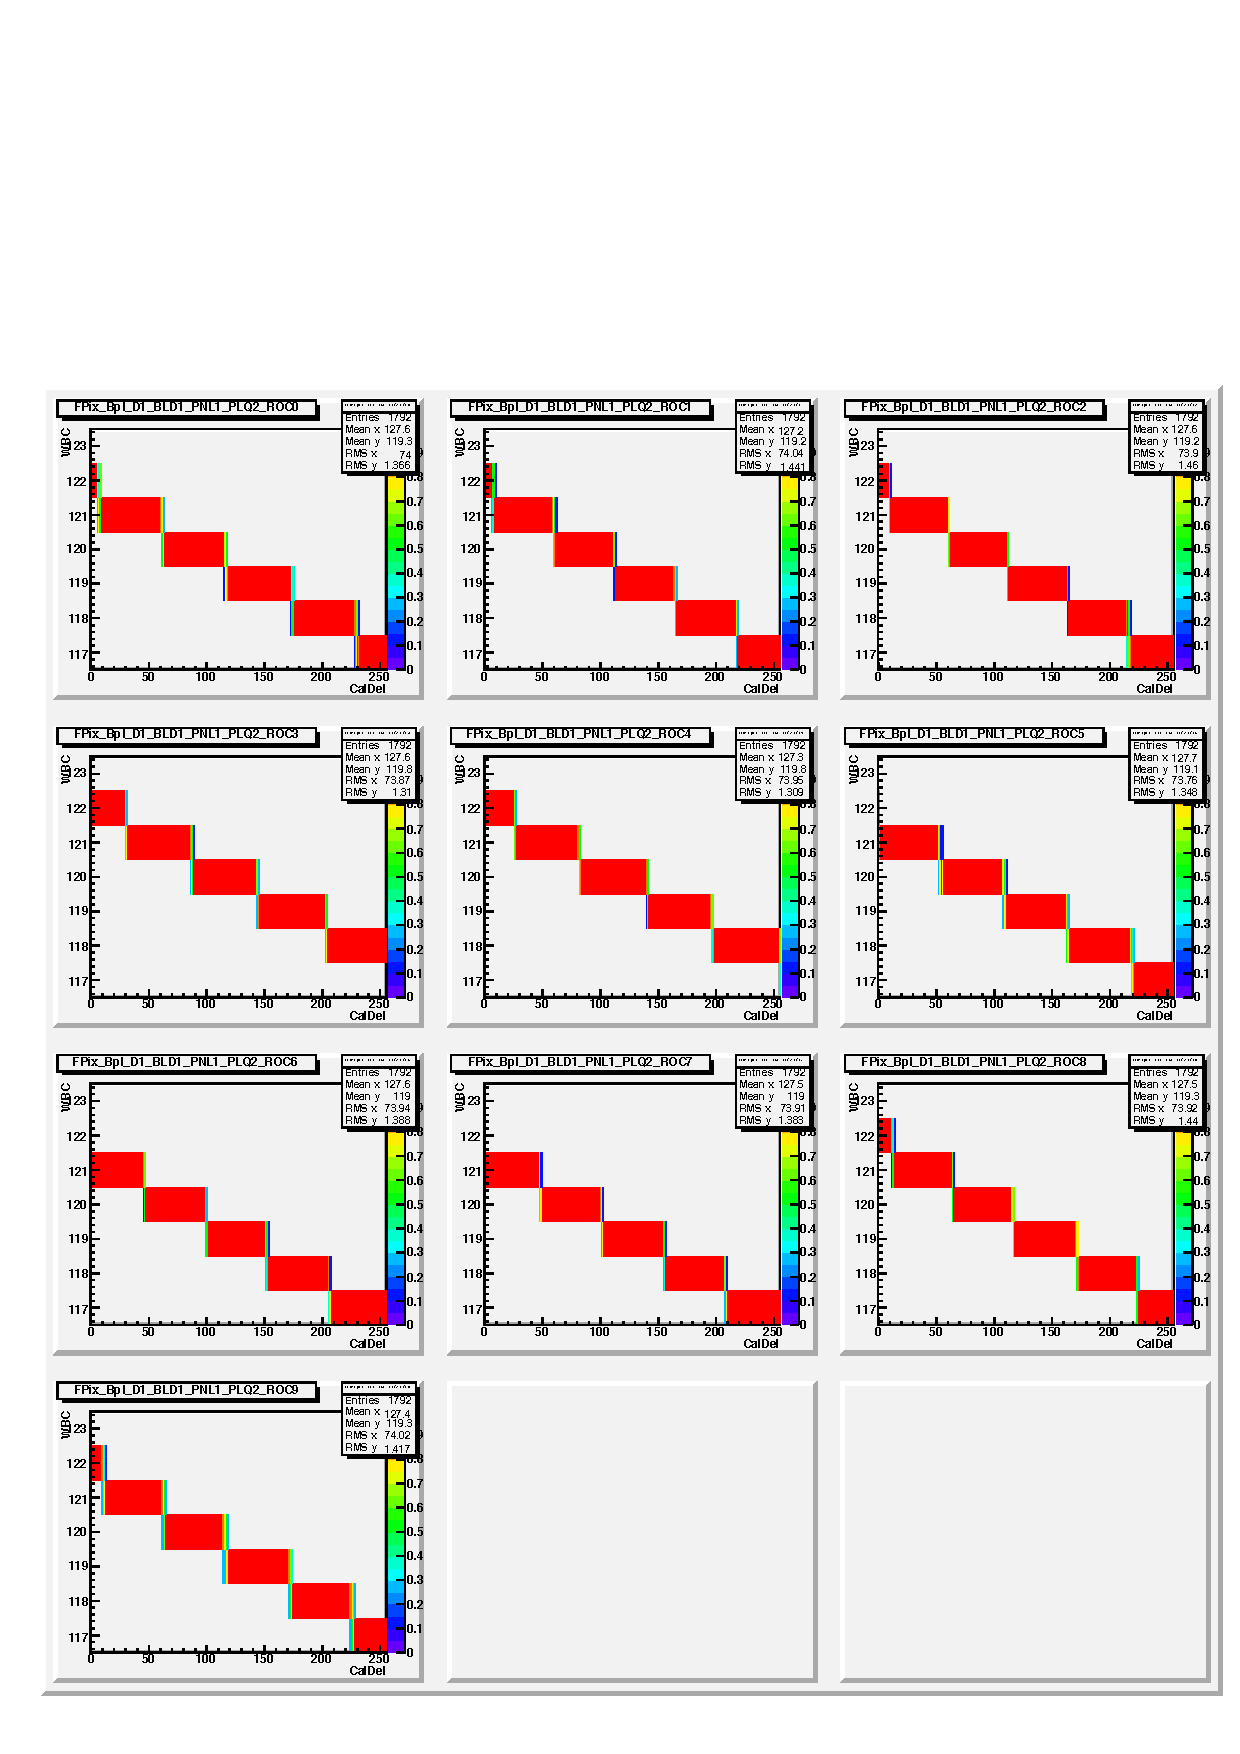
\includegraphics[width=\linewidth]{CalDelCalibration.pdf}
\end{center}
\caption{The efficiency as a function of WBC vs CalDel.}
\label{fig:caldel}
\end{figure}



\subsubsection{Example}

An example of a configuration file for the CalDel
calibration is shown below:

\begin{verbatim}
Mode: CalDelCalibration
Rows:
10 | 20
Cols:
10 | 20
VcalHigh
Scan: WBC 117 123 1
Scan: CalDel 0 255 1
Set: Vcal 250
Repeat: 2
ToCalibrate:
+ all
\end{verbatim}

If you want to just scan over WBC to find the
right WBC value you can use a configuration
that sets CalDel to a fixed value:

\begin{verbatim}
Mode: CalDelCalibration
Rows:
10 | 20
Cols:
10 | 20
VcalHigh
Scan: WBC 117 123 1
Scan: CalDel 100 100 1
Set: Vcal 250
Repeat: 2
ToCalibrate:
+ all
\end{verbatim}

\subsection{Idigi vs. Vsf}

In this 'calibration' we scan Vsf and measure the
digital current. This is not really a calibration
as we don't determine any settings from this. Rather
what we do is to find a maximum Vsf setting that we
will use. If Vsf is too large the digital current
increases. In the configuration for this calibration
you can set the maximum increase in Idigi that
you allow using the parameter IdigiMax (units are
in mA). IdigiMax is currently set to 7 mA.

\subsubsection{Output}

This calibration produces the object
PixelMaxVsf which is used in the calibration that
determines Vsf to optimize the linearity.
In addition this calibration produces output
in a file called idigi.dat. Using the root
script idigi.c you can generate plots as
shown in Fig.~\ref{fig:IdigivsVsf}.

\begin{figure}
\begin{center}
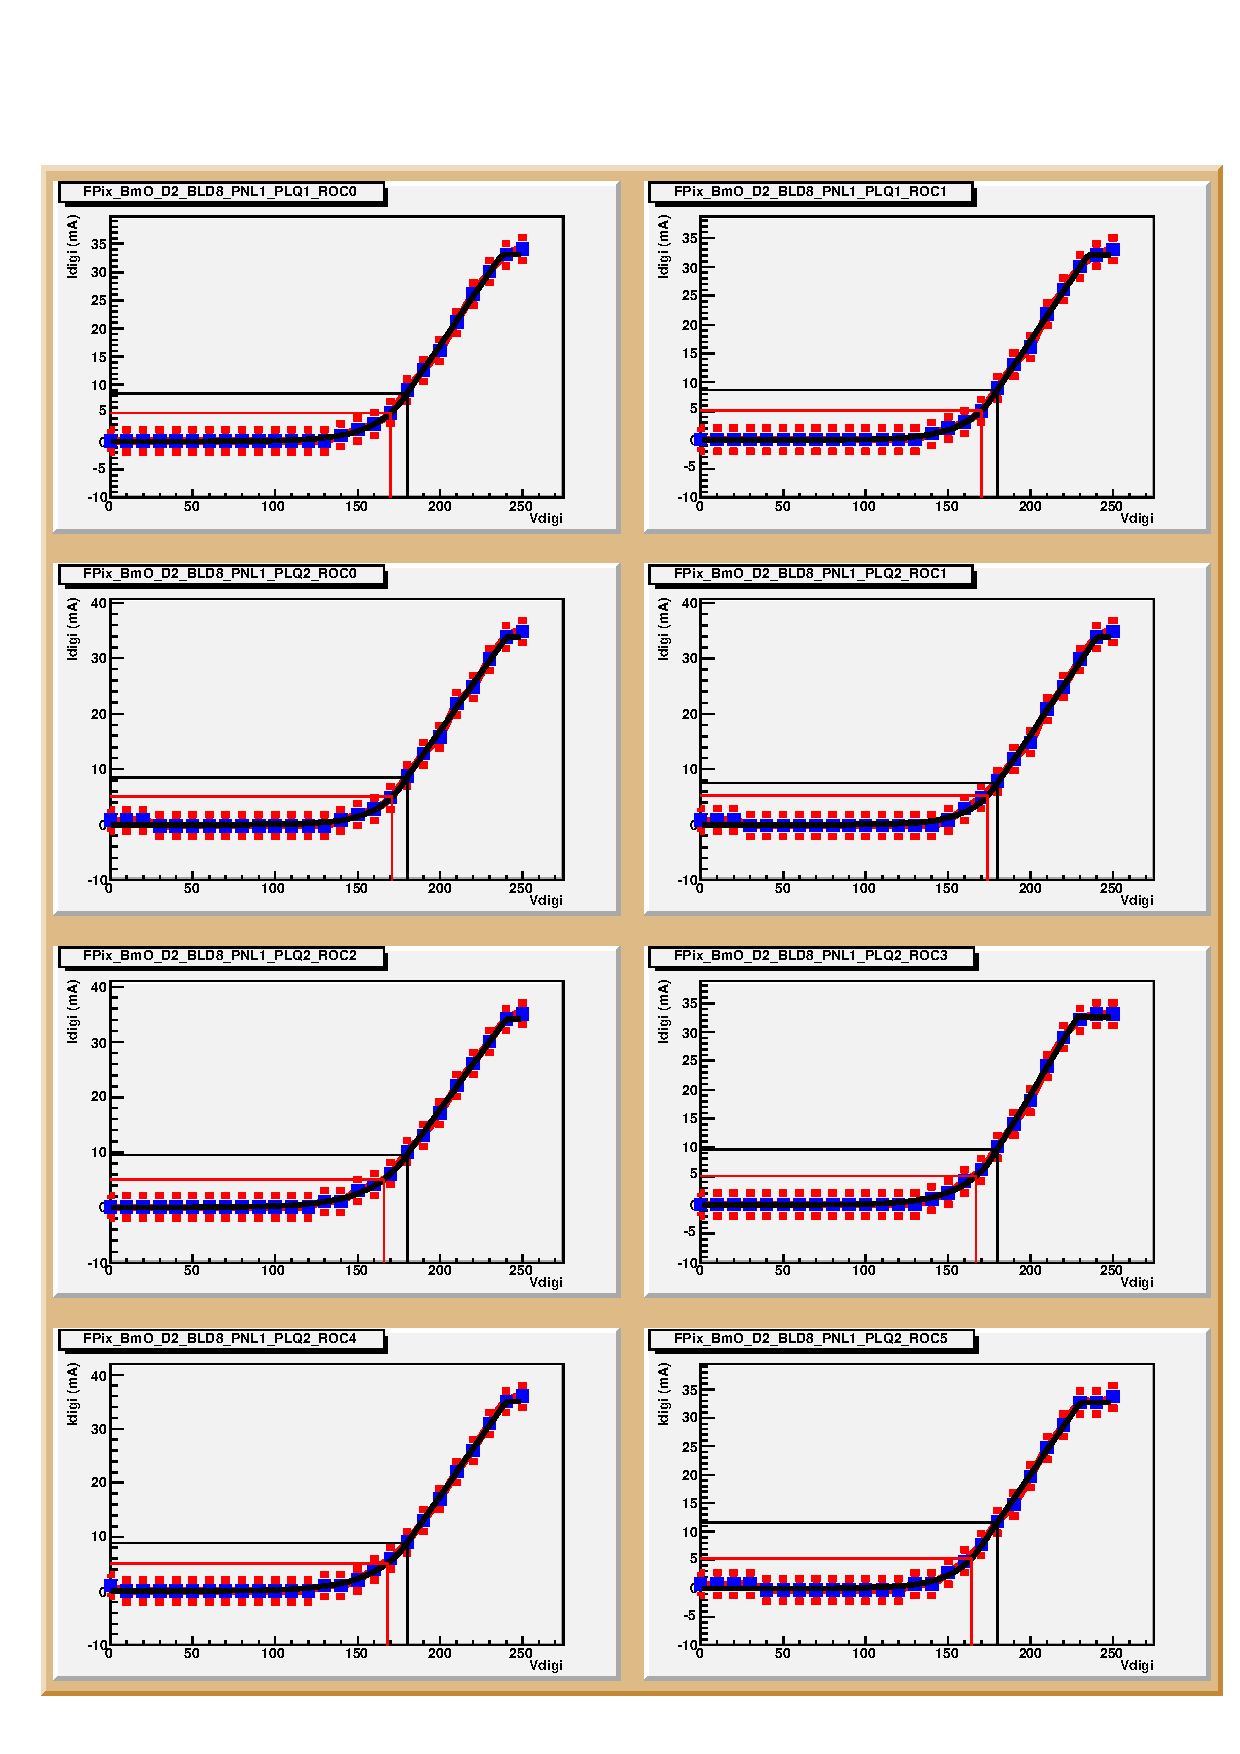
\includegraphics[width=\linewidth]{idigi1}
\end{center}
\caption{The digital current is shown as a function of Vsf. }
\label{fig:IdigivsVsf}
\end{figure}

\subsubsection{Example}

The configuration used for the digital scan
looks like
\begin{verbatim}
Mode:  Idigi
Rows:
Cols:
Vcal:
200 200 5
Repeat:
1
ToCalibrate:
+ all
\end{verbatim}

\subsection{Linearity vs.~Vsf} \label{sec:LinearityVsVsf}

The ROC DAC setting \verb|Vsf| affects the linearity of the pixel response vs.~received charge; larger values improve linearity.  \verb|Vsf| also affects the digital current, with higher values increasing the current.  We have implemented two algorithms to set \verb|Vsf| at a value that gives good linearity without drawing excessive power.  The first, described in this section, is the algorithm developed at PSI.

\subsubsection{Introduction and discussion}

This algorithm measures linearity from scans of pulse height vs.~\verb|Vcal| at different values of \verb|Vsf|.  Examples of these scans are shown in Fig.~\ref{fig:PH_vs_Vcal_scans}.

\begin{figure}
\begin{center}
 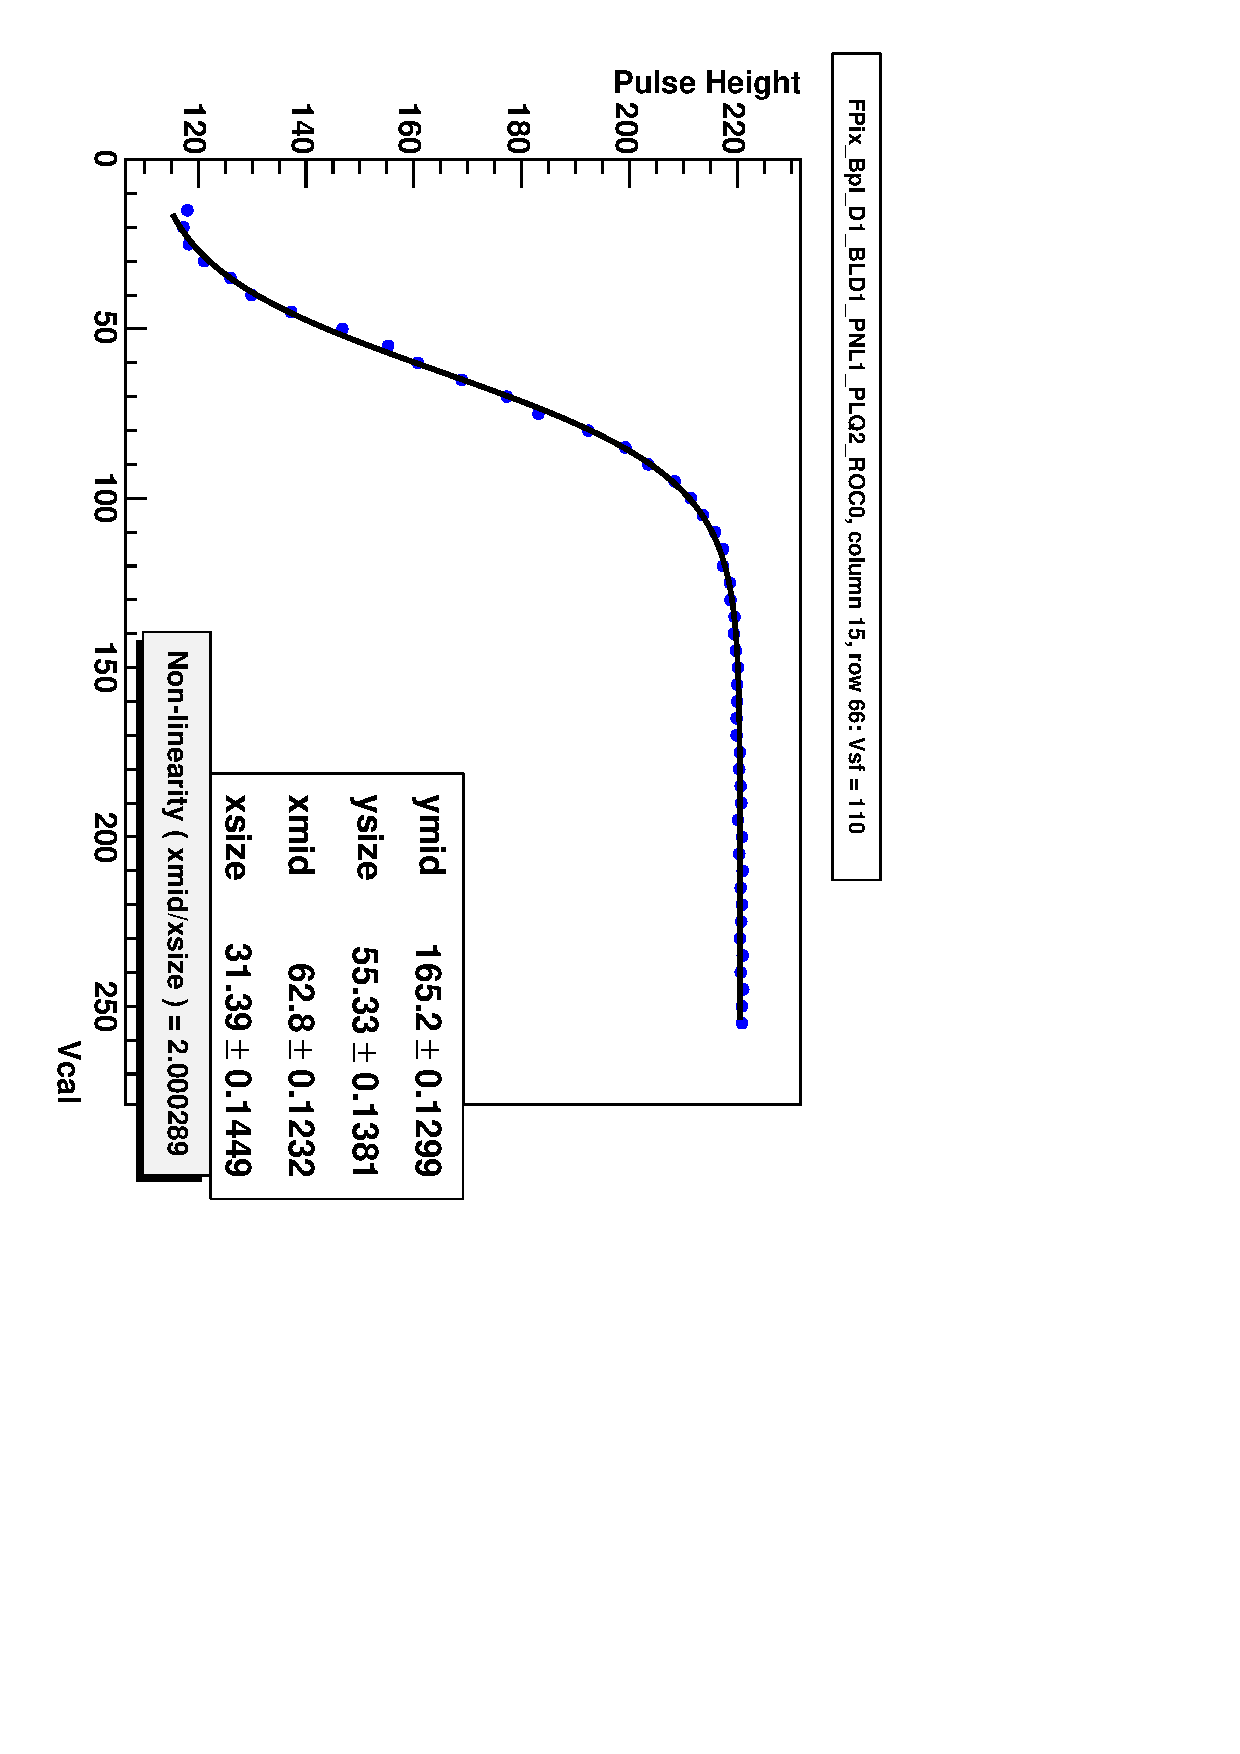
\includegraphics[angle=90,width=0.49\textwidth]{PH_vs_Vcal_poorLinearity.pdf}
 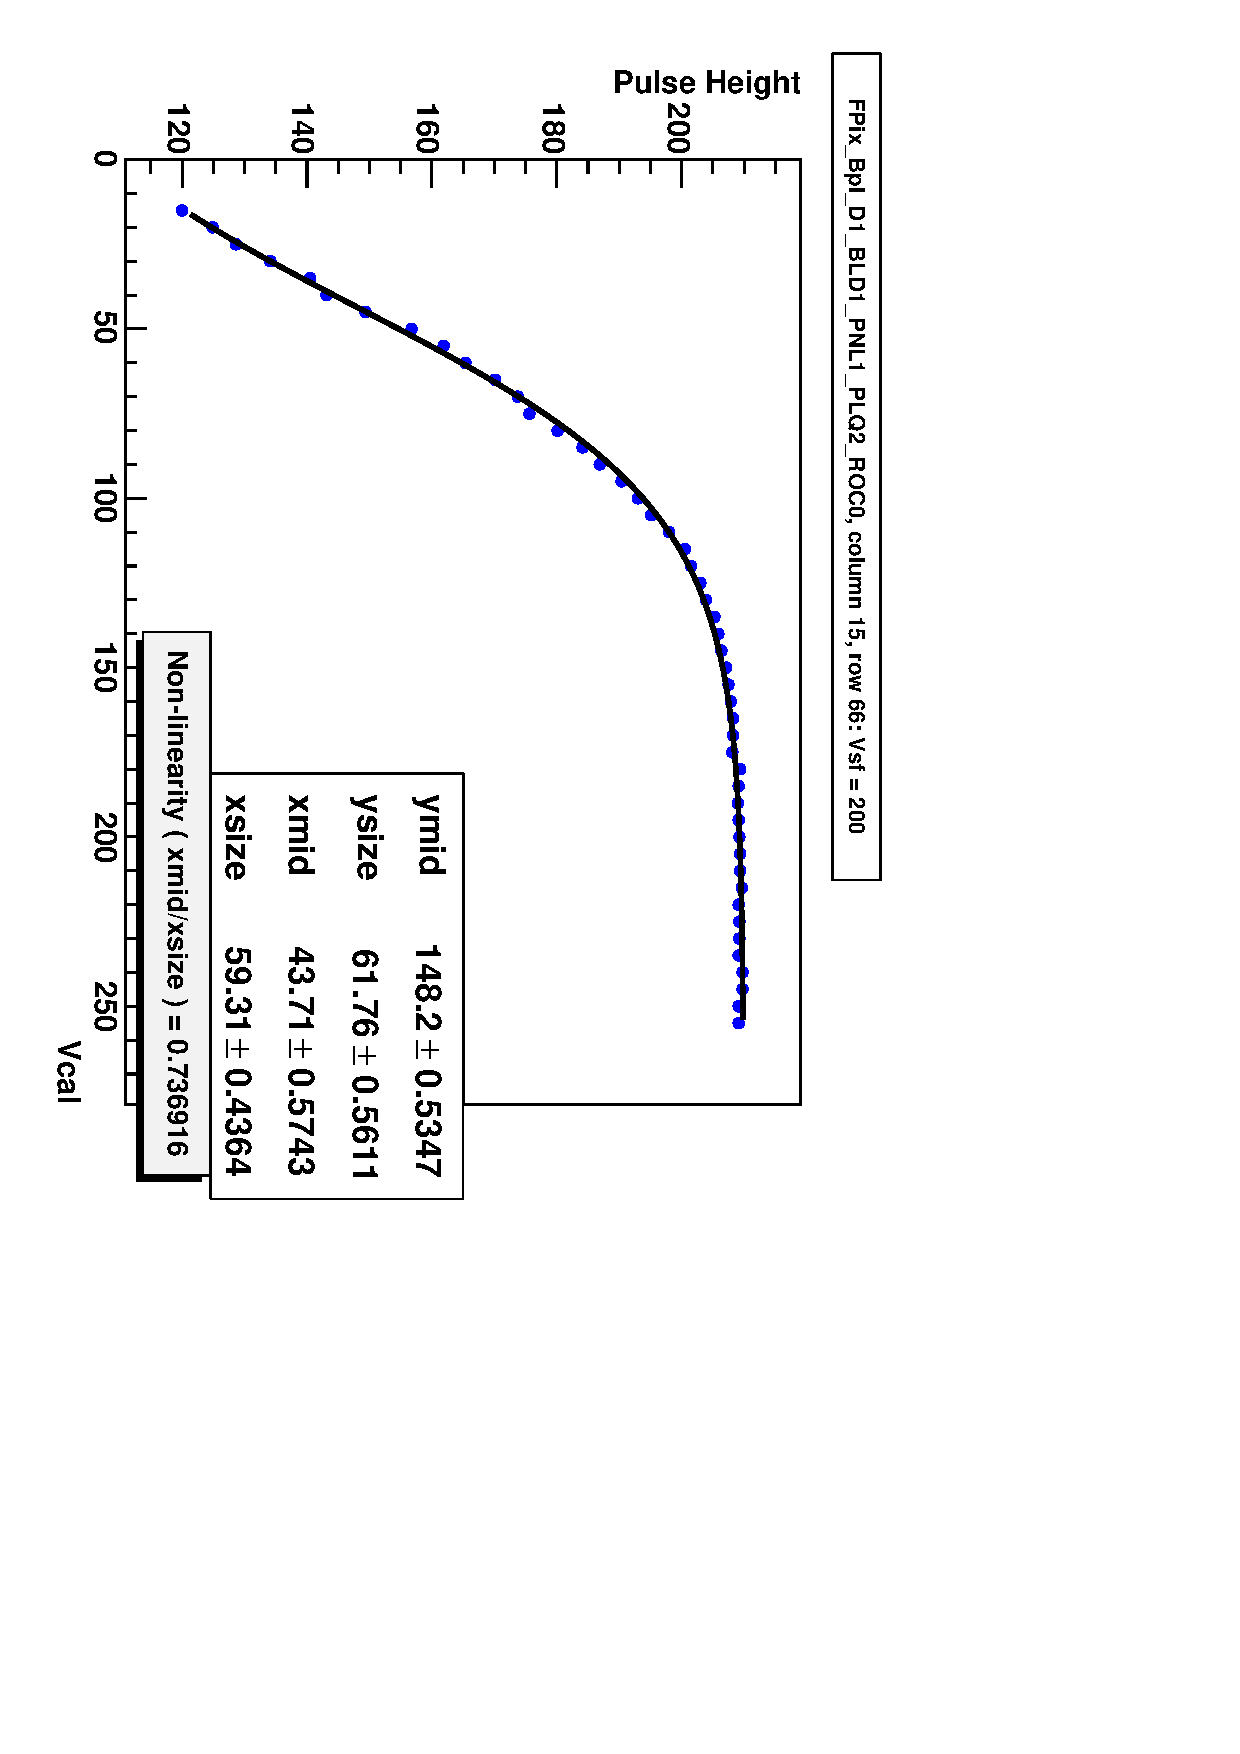
\includegraphics[angle=90,width=0.49\textwidth]{PH_vs_Vcal_goodLinearity.pdf}
\end{center}
\caption{Scans of pulse height vs.~Vcal at different values of Vsf.  The scan on the left has poor linearity, and the scan on the right has good linearity.  (Note that these scans come from a detector which has no voltage bias, so the received charge and the slope of the linear section are lower than in a biased detector.)}
\label{fig:PH_vs_Vcal_scans}
\end{figure}

To quantify the degree of nonlinearity, the scan data are fit with a function
\begin{equation} \label{eq:tanh}
PH = f(Vcal) = y_{\rm mid} + y_{\rm size} \times \tanh \left( \frac{Vcal - x_{\rm mid}}{x_{\rm size}} \right)
\end{equation}
where $PH$ is the recorded pulse height, $Vcal$ is the input, $(x_{\rm mid},y_{\rm mid})$ is the point at the center of the quasi-linear rise region of the hyperbolic tangent, $x_{\rm size}$ is the horizontal scale of the quasi-linear region, and $y_{\rm size}$ is the vertical scale of that region.

From this fit, the degree of nonlinearity can be quantified in different ways.  The simpler nonlinearity parameter, used by PSI and used by default in this calibration, is $x_{\rm mid}/x_{\rm size}$.  When this parameter is small, it means that \verb|Vcal| = 0 lies within the quasi-linear rise region, and hence the response is linear for small amounts of injected charge.  PSI has used $x_{\rm mid}/x_{\rm size} = 1.4$ as the cutoff -- values below 1.4 indicate good linearity.

An alternate nonlinearity parameter is
\begin{equation} \label{eq:nonlinearityIntegral}
\frac{1}{2} \int_{Vcal_{\rm min}}^{Vcal_{\rm max}} dVcal \left| \frac{f''(Vcal)}{f'(Vcal)} \right|
\end{equation}
where $f(Vcal)$ is the hyperbolic tangent function in Eq.~(\ref{eq:tanh}).  This integral is a measure of the vertical change due to curvature divided by the vertical change due to slope over the range of the integral.  The limits of the integral should be chosen to include the range for which we want good linearity.  By default the limits go from \verb|Vcal| = 50 to \verb|Vcal| = 400 in low-scale \verb|Vcal| units, or from 50/7 to 400/7 in high-scale units.  This integral can be evaluated analytically.

Figure~\ref{fig:nonlinearityPlots} shows scans of both measures of nonlinearity vs.~\verb|Vsf|.  As seen in the plots, they give similar shapes.  This calibration allows the user to use either measure; the default is $x_{\rm mid}/x_{\rm size}$.

\begin{figure}
\begin{center}
 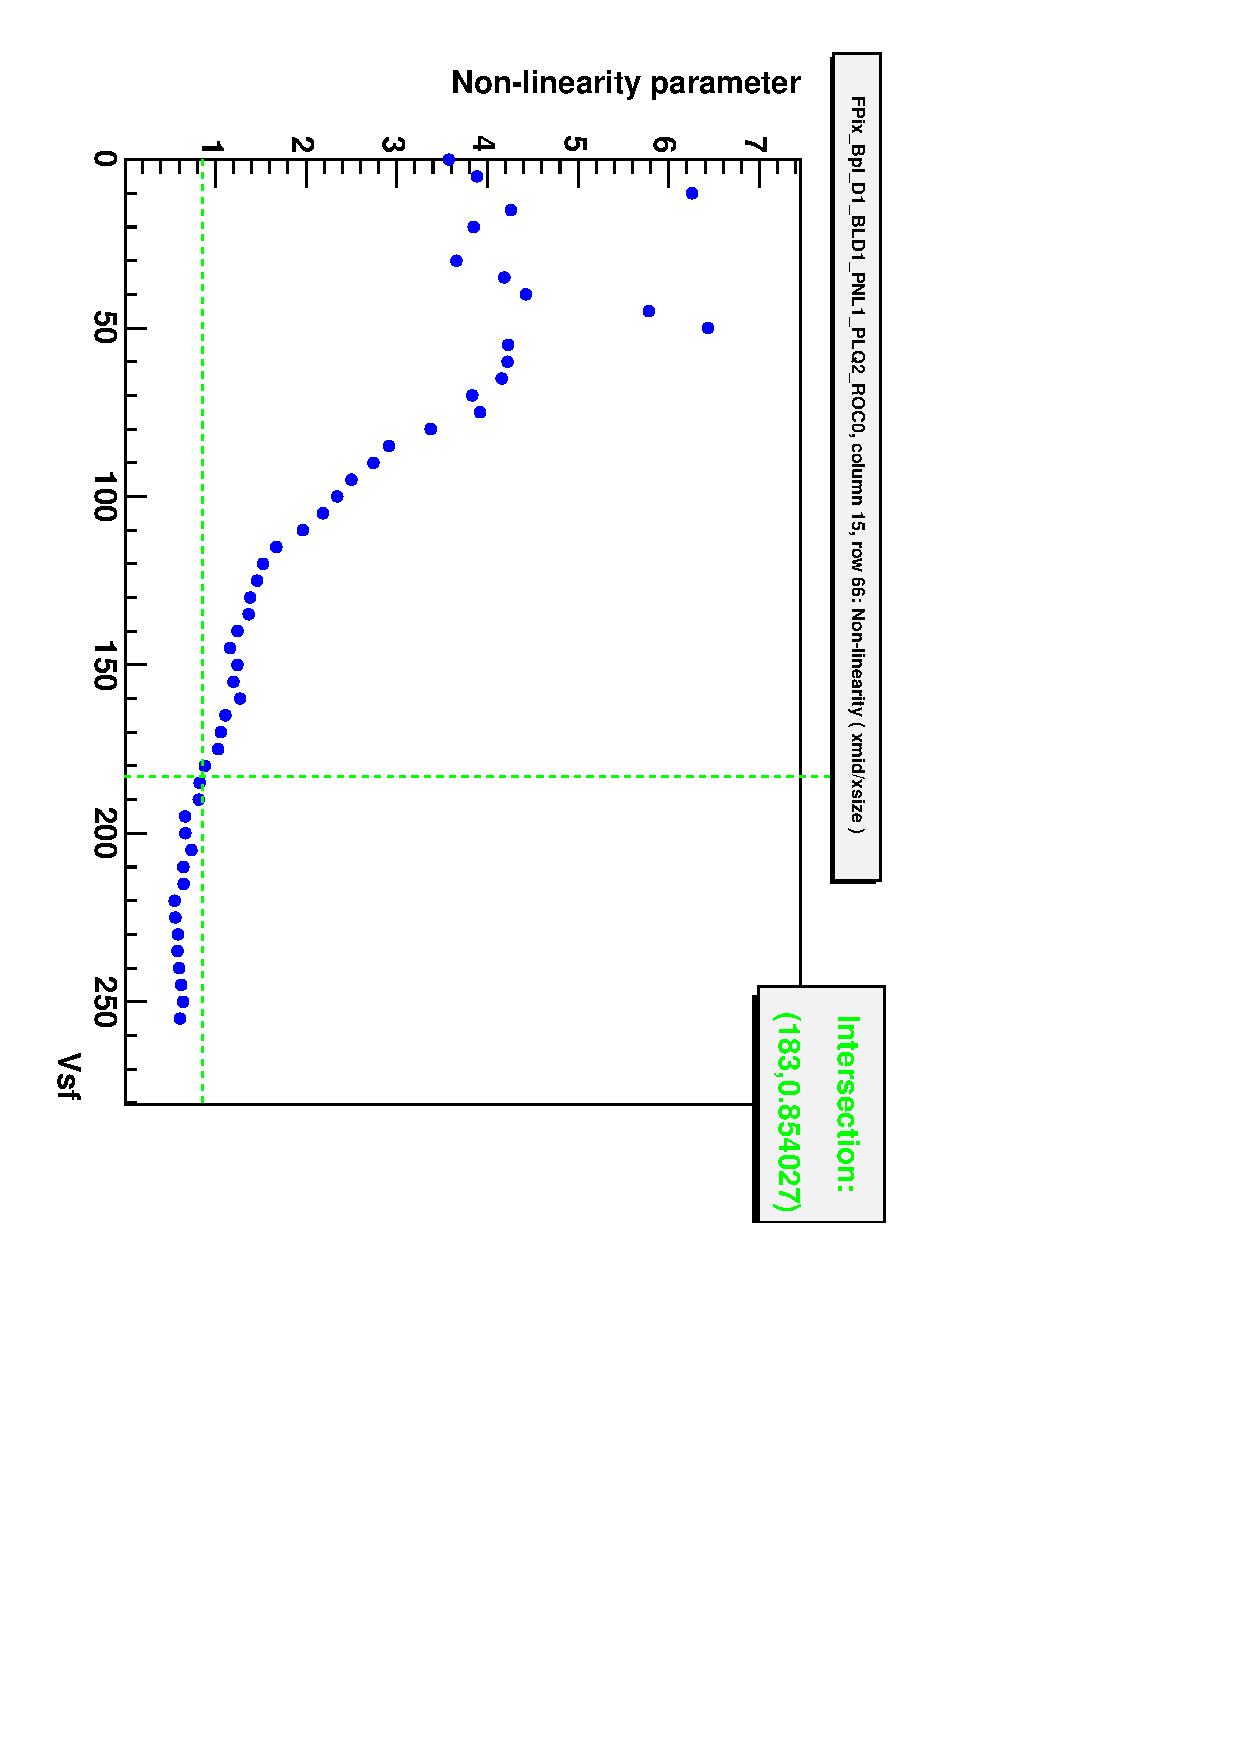
\includegraphics[angle=90,width=0.49\textwidth]{nonlinearityPlot_xmidOverXsize.pdf}
 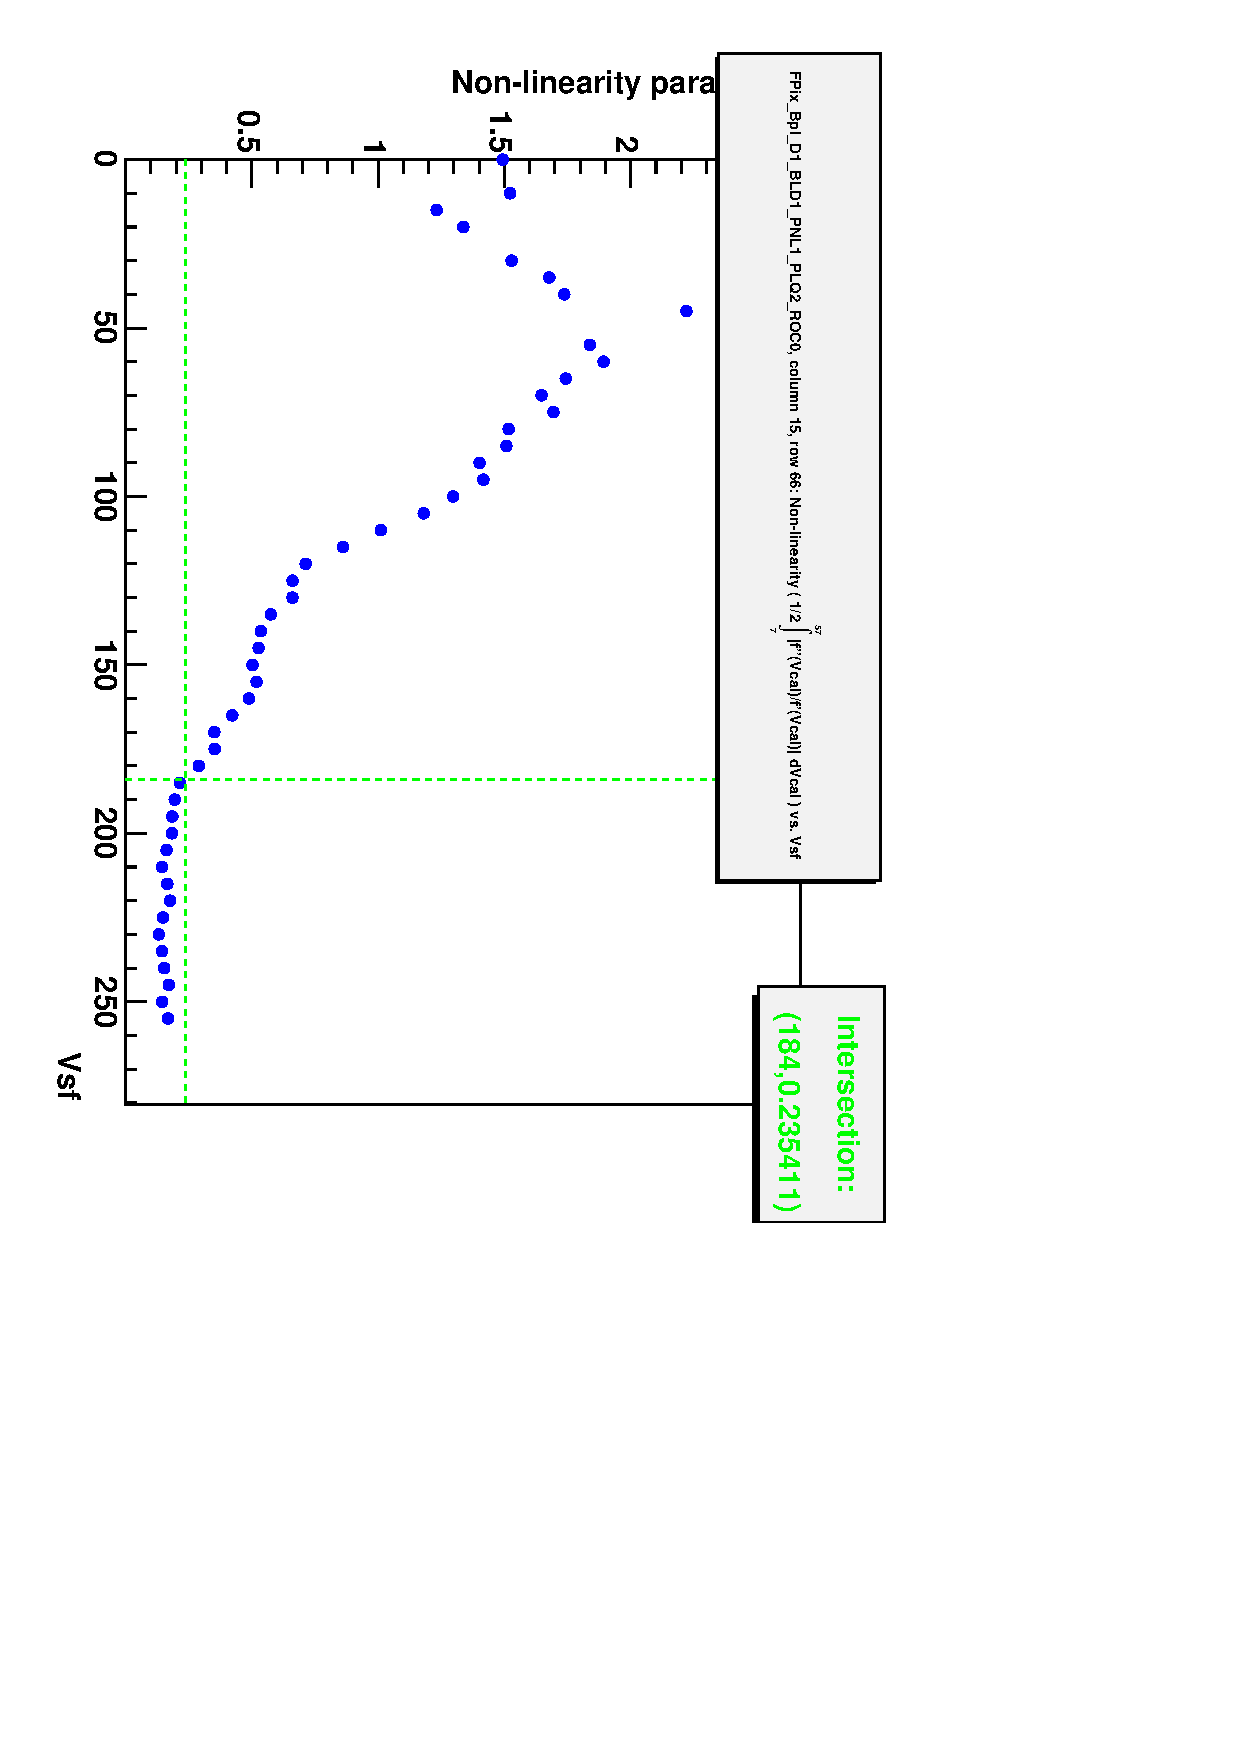
\includegraphics[angle=90,width=0.49\textwidth]{nonlinearityPlot_integral.pdf}
\end{center}
\caption{Plots of nonlinearity vs.~Vsf.  On the left, nonlinearity is measured by $x_{\rm mid}/x_{\rm size}$, and on the right, it is measured by the integral in Eq.~(\ref{eq:nonlinearityIntegral}).}
\label{fig:nonlinearityPlots}
\end{figure}

\subsubsection{Linearity vs.~Vsf calibration steps}

This calibration consists of the following steps:
\begin{enumerate}
\item Scan \verb|Vcal| and \verb|Vsf| according to the calibration's configuration.  On each trigger, read out data from each FED's FIFO3.  Record the pulse height, keeping separate scans for different pixels.
\item For each scan of pulse height vs.~\verb|Vcal| (for a given ROC, pixel, and \verb|Vsf| value), fit with the function in Eq.~(\ref{eq:tanh}).  A plot of each scan and fit is written to a ROOT file (see Fig.~\ref{fig:PH_vs_Vcal_scans}).  If the fit is successful, compute the nonlinearity parameter (either $x_{\rm mid}/x_{\rm size}$ or the integral in Eq.~(\ref{eq:nonlinearityIntegral})) and add it to a scan of nonlinearity vs.~\verb|Vsf| for that ROC and pixel.  This scan is also written to a ROOT file (see Fig.~\ref{fig:nonlinearityPlots}).
\item For each scan of nonlinearity vs.~\verb|Vsf|, determine an optimal \verb|Vsf|.  This is done by finding the highest \verb|Vsf| where the scan intersects a nonlinearity threshold.  This threshold may be either absolute or relative, according to the parameter ``\verb|absoluteNonlinearityThreshold|".  If absolute, the threshold is set by the parameter ``\verb|nonlinearityThreshold|".  If relative, the threshold is the value of the nonlinearity at the highest \verb|Vsf| in the scan, multiplied by the parameter ``\verb|nonlinearityThreshold|".
\item For each ROC, examine the optimal \verb|Vsf|s on the various pixels.  If there are at least 4 pixels, discard any \verb|Vsf| outliers.  After any discarding, average the \verb|Vsf| values to determine the \verb|Vsf| setting for that ROC.
\item Compare the \verb|Vsf| setting on each ROC to the maxVsf setting in the configuration.  If the setting from this calibration exceeds the maximum, reduce \verb|Vsf| to the maximum allowed.
\item Write out new ROC configuration files for the successfully-calibrated
ROCs with the new \verb|Vsf| settings.
\item Print out a summary.
\end{enumerate}

\subsubsection{Parameters}
A number of parameters in \verb|calib.dat| may be used to control the
calibration.

The various ``standard" parameters are used in this calibration.  The
``\verb|Repeat:|" parameter determines the number of triggers in each step
of the scan.  The ROC list is used to determine which ROCs are calibrated.

The scan ranges are specified by lines like
\begin{verbatim}
Scan: Vcal  0 255 5
Scan: Vsf   0 255 5 mix
\end{verbatim}
which specify the scan range and step size.  The ``\verb|mix|'' flag must be enabled for \verb|Vsf| (or alternatively SingleROC mode must be used); otherwise the calibration will abort.

The hits specified in \verb|Rows:| and \verb|Columns:| will be
used.  One scan is taken for each pixel with hits.  At most two hits per pixel pattern may be specified (or alternatively SingleROC mode must be used); otherwise the calibration will abort.  The reason for this restriction is that the FED's spy FIFO3 will overflow if each ROC connected to it has more than two hits.

Some optional parameters may also be set.  All have default values which will
be used if the parameter is not set.  These parameters, their defaults, and
their functionality are given in Table~\ref{tab:LinearityVsVsfParameters}.

\begin{table}
\centering
\caption{Optional parameters for linearity vs. Vsf calibration.}
\label{tab:LinearityVsVsfParameters}
\begin{tabular}{l@{~~~~}l@{~~~~}l}
\hline
\hline
Parameter & Default & Description \\
\hline
absoluteNonlinearityThreshold     & yes   & Whether the nonlinearity threshold is an \\
                                  &       &   absolute number, or a multiple of the \\
                                  &       &   nonlinearity parameter at maximum \verb|Vsf| \\
nonlinearityThreshold             & 1.4   & Value of the nonlinearity threshold \\
useIntegrated2ndOver1stDerivative & no    & Whether to use the integral in Eq.~(\ref{eq:nonlinearityIntegral}) for the \\
                                  &       &   nonlinearity parameter, instead of $x_{\rm mid}/x_{\rm size}$ \\
integralMinVcal                   &  50/7 & Lower \verb|Vcal| bound of the integral (if used) \\
integralMaxVcal                   & 400/7 & Upper \verb|Vcal| bound of the integral (if used) \\
\hline
\hline
\end{tabular}
\end{table}

\subsection{Vsf and VHldDel}

\subsubsection{Introduction and discussion}

We have also implemented the Renaissance algorithm for determining the ROC DAC settings \verb|Vsf| and \verb|VHldDel|.  Figure~\ref{fig:PHvsVHldDel} shows plots of pulse height vs.~\verb|VHldDel| at low, medium, and high values of \verb|Vsf|, with \verb|Vcal| = 250 on the low scale.  A good \verb|Vsf| value is one for which this curve rises and then falls so that the pulse heights at the two endpoints (lowest and highest \verb|VHldDel|) are equal.  Figure~\ref{fig:PHvsVHldDel} also includes a plot of these endpoints as a function of \verb|Vsf|; the rightmost intersection point is the \verb|Vsf| value chosen.  Low values of \verb|Vsf|, below $\sim$90, produce garbage output.

\begin{figure}
\begin{center}
 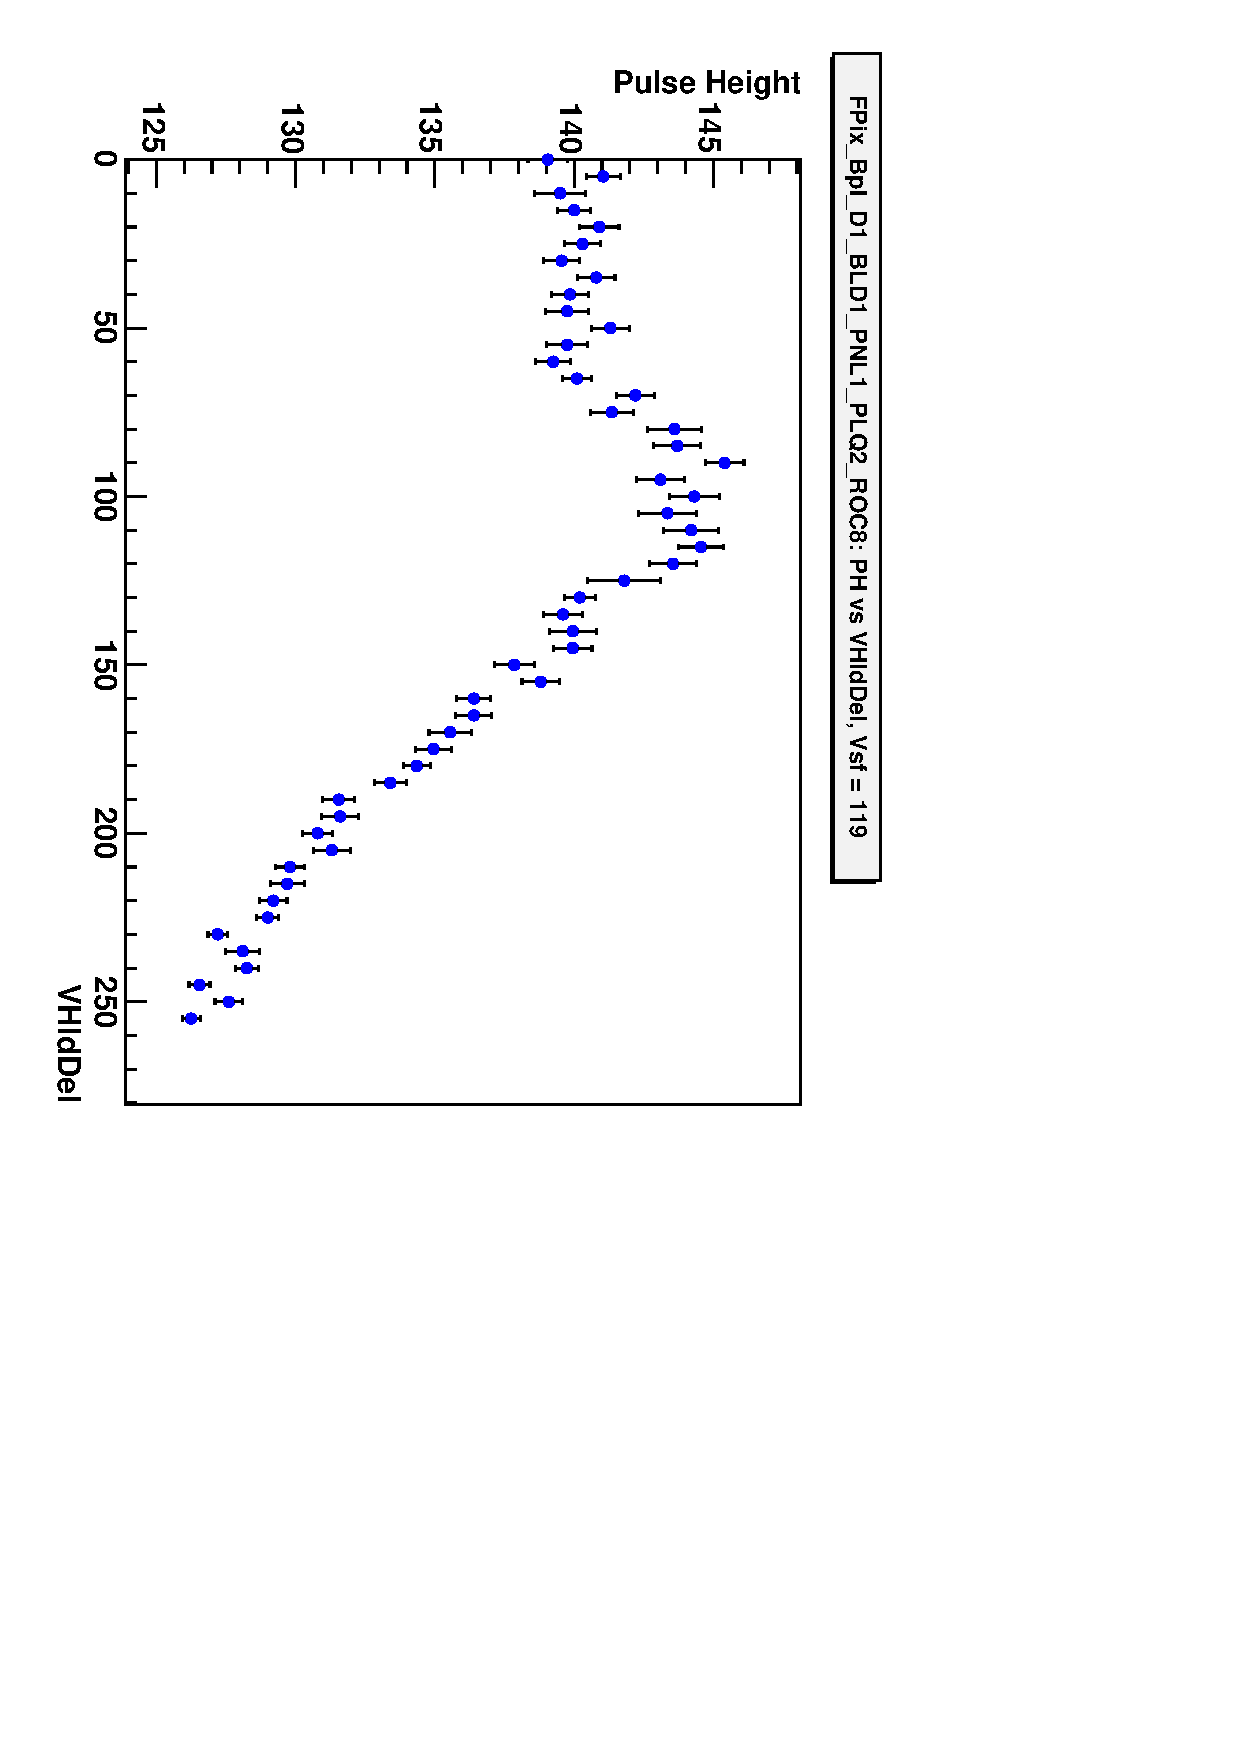
\includegraphics[angle=90,width=0.32\textwidth]{PH_vs_VHldDel_Vsf119.pdf}
 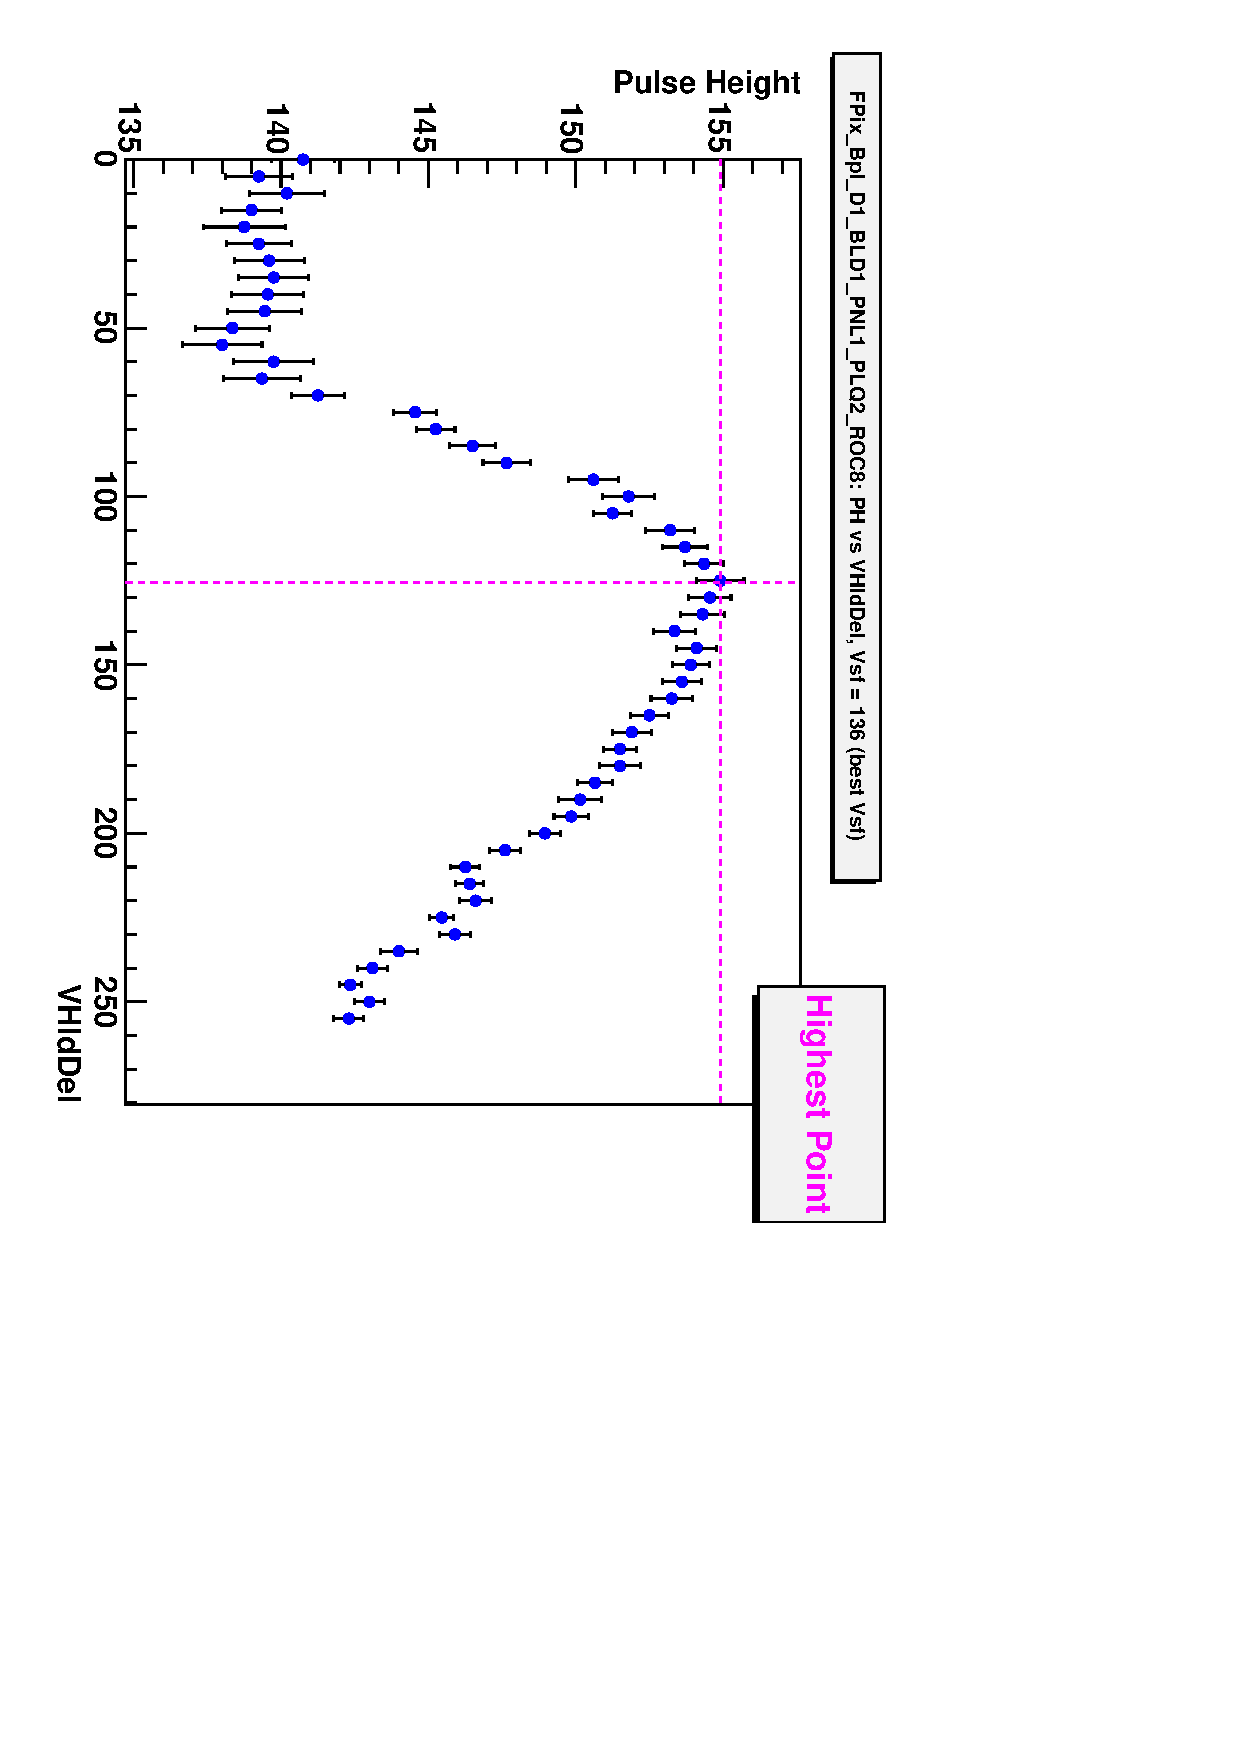
\includegraphics[angle=90,width=0.32\textwidth]{PH_vs_VHldDel_Vsf136.pdf}
 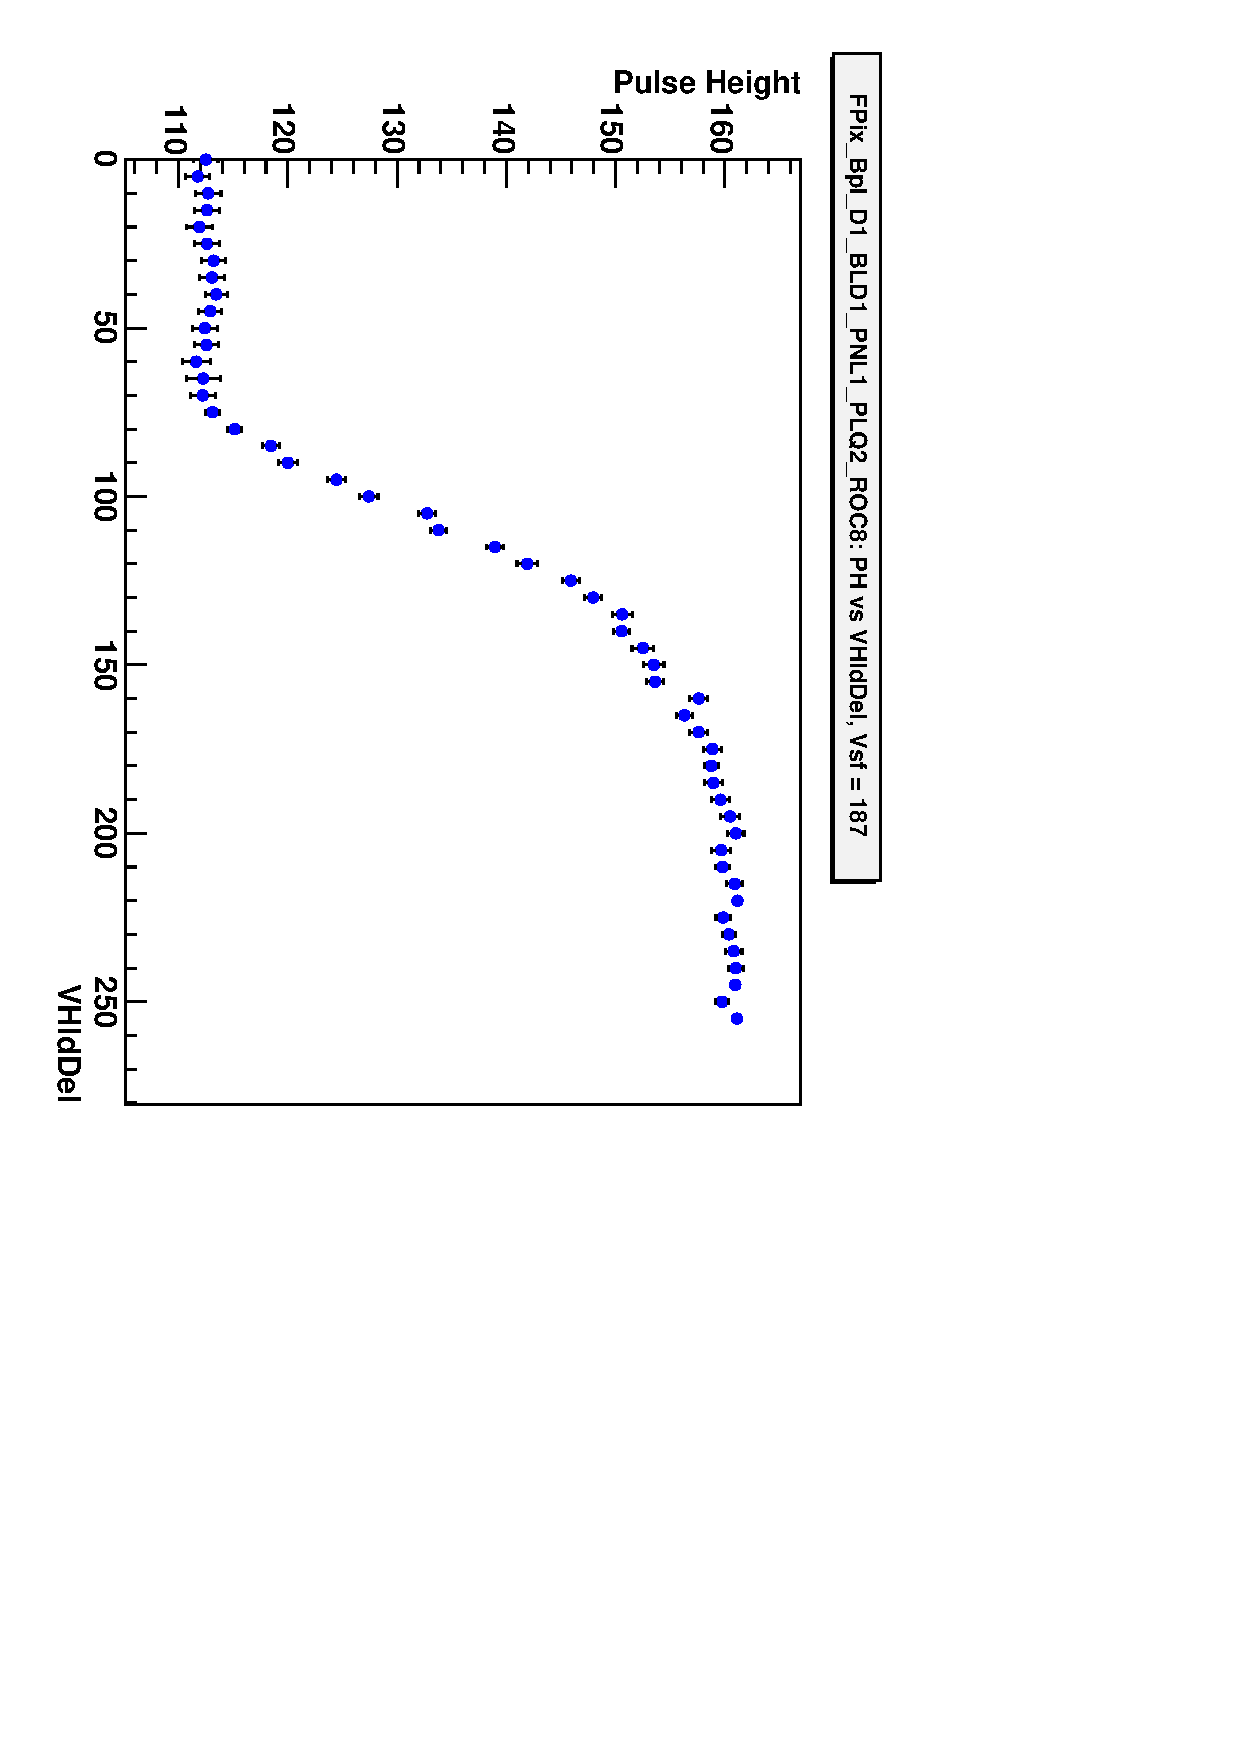
\includegraphics[angle=90,width=0.32\textwidth]{PH_vs_VHldDel_Vsf187.pdf}
 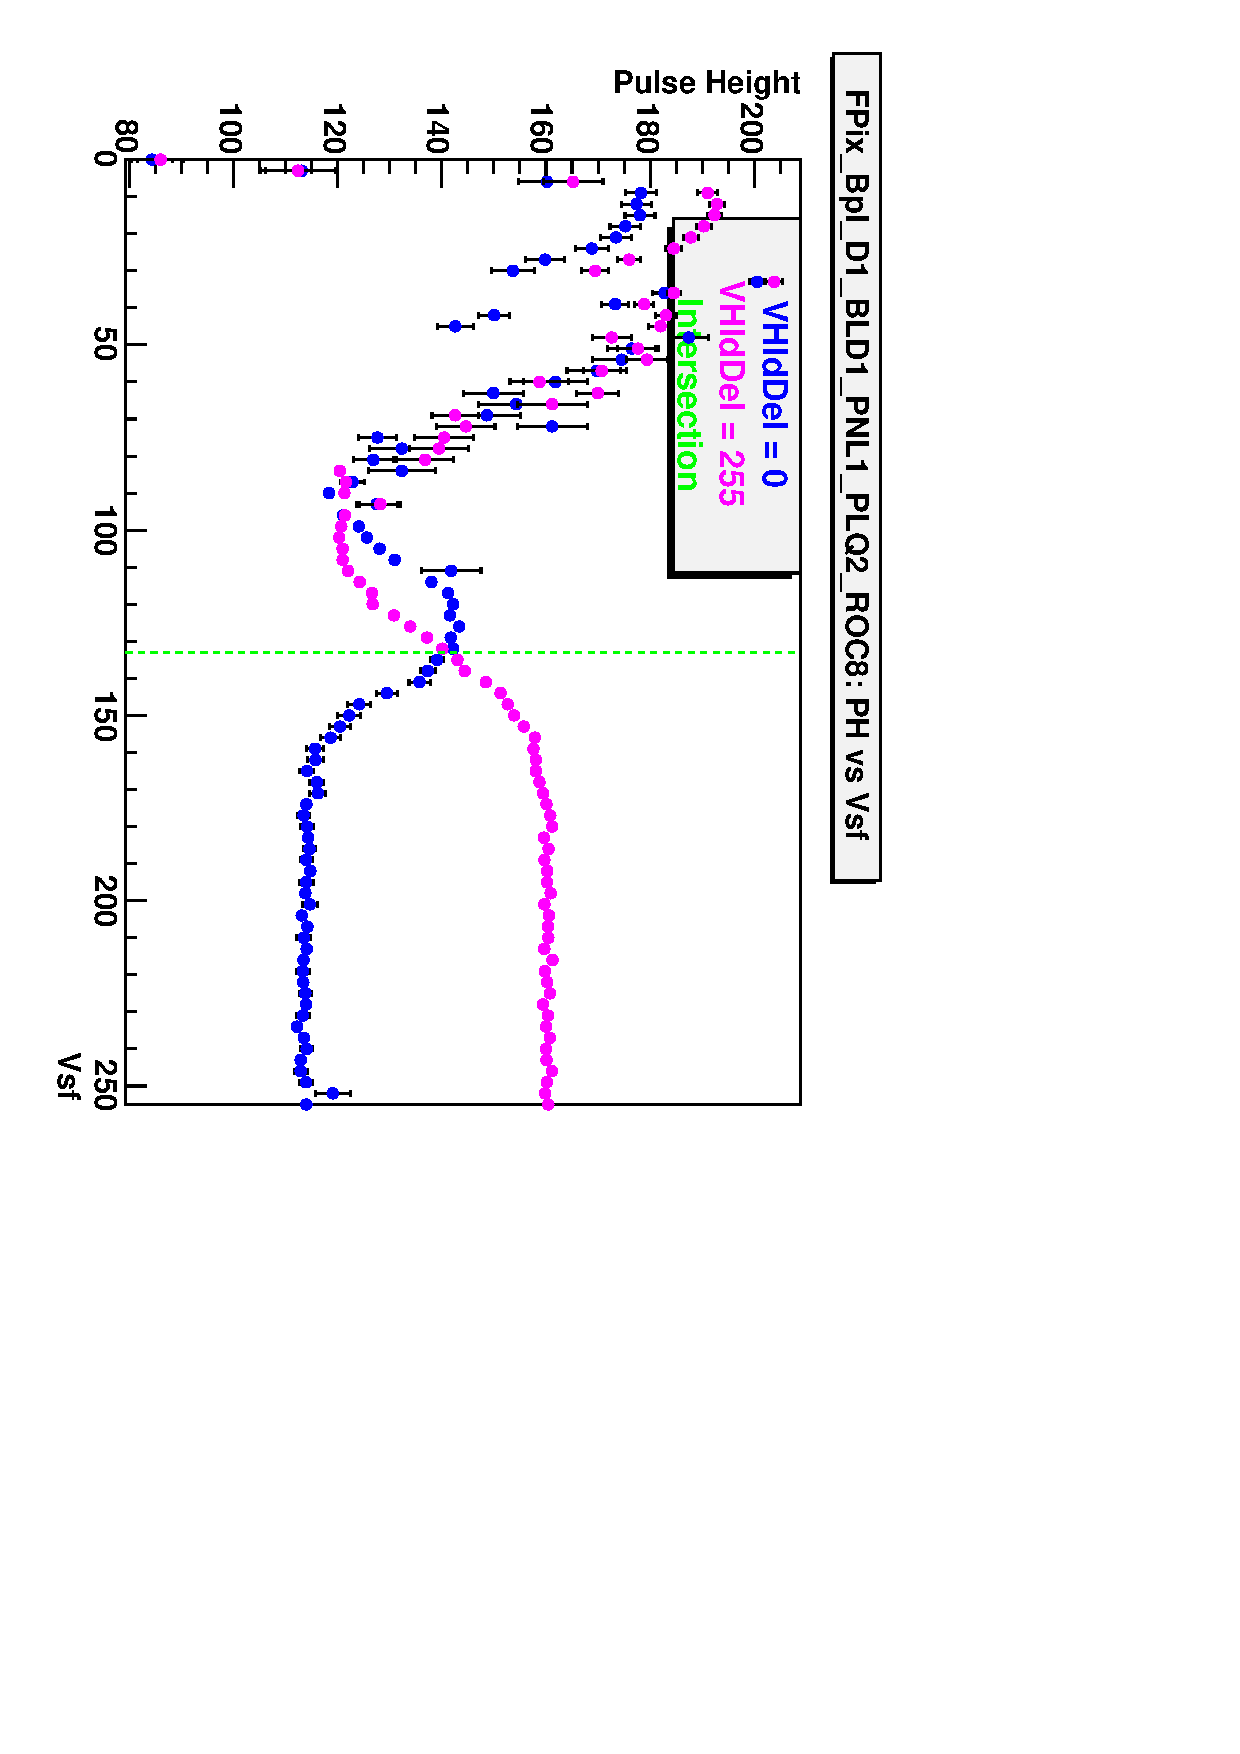
\includegraphics[angle=90,width=0.49\textwidth]{PH_vs_Vsf.pdf}
\end{center}
\caption{\emph{Top row:} Pulse height vs. VHldDel at low, medium, and high values of Vsf, with Vcal = 250 on the low scale.  As Vsf increases, the right endpoint increases.  The best Vsf value is the one for which the pulse heights measured at VHldDel = 0 and VHldDel = 255 are equal.  \emph{Bottom plot:} Pulse height at the endpoints of these plots, as a function of Vsf.  Low values of Vsf produce garbage output.}
\label{fig:PHvsVHldDel}
\end{figure}

After choosing a \verb|Vsf| value, \verb|VHldDel| should be set to the value that maximizes the pulse height.

When charge is injected with \verb|Vcal| = 250 on the low scale, these \verb|Vsf| and \verb|VHldDel| settings are found to give good linearity in pulse height vs.~injected charge, while not drawing too much power.

This procedure may be done in one calibration run, or it may be split into two -- the first to determine \verb|Vsf| and the second to determine \verb|VHldDel|.  Splitting into two runs is better because (1) it requires fewer scan points and (2) when the best \verb|Vsf| is a value interpolated between two scan points, the scan over \verb|VHldDel| will take place at that value instead of at the nearest \verb|Vsf| scan point.  The same calibration code can calibrate both DACs at once, or either one of them; calibration parameters determine which mode is used.  This is described in more detail below.

If the PSI algorithm described in Sec.~\ref{sec:LinearityVsVsf} is used to determine \verb|Vsf|, \verb|VHldDel| should be set with the algorithm used here -- maximizing pulse height at the chosen \verb|Vsf|.

\subsubsection{Vsf and VHldDel calibration steps}

This calibration consists of the following steps:
\begin{enumerate}
\item Scan \verb|Vsf| and \verb|VHldDel| according to the calibration's configuration.  On each trigger, read out data from each FED's FIFO3.  Record the pulse height.  If multiple pixels are enabled, average all of their pulse heights on each ROC.
\item If \verb|Vsf| was scanned, determine the best \verb|Vsf|.  To do this, make plots of pulse height vs.~\verb|Vsf| for the lowest \verb|VHldDel| scan value and for the highest \verb|VHldDel| scan value.  Take the rightmost intersection (the one at the largest \verb|Vsf|) as the best \verb|Vsf| value.  (When finding this intersection, interpolate between scan points.)  If the intersection point exceeds the maxVsf setting in the configuration for that ROC, reduce \verb|Vsf| to the maximum allowed.
\item If there are 3 or more \verb|VHldDel| scan points, determine the best \verb|VHldDel|.  If \verb|Vsf| was scanned, examine the scan of pulse height vs.~\verb|VHldDel| for the \verb|Vsf| scan point closest to the value chosen.  If \verb|Vsf| was not scanned, a scan of pulse height vs.~\verb|VHldDel| was taken at the \verb|Vsf| value stored in the configuration; examine this scan.  Find the scan point with the highest pulse height.  Calculate the parabola that passes through this point and the two adjacent points, and take the maximum of this parabola as the best \verb|VHldDel| value.  (If the highest point is an endpoint, use the endpoint as the best \verb|VHldDel|.)
\item Write out new ROC configuration files for the successfully-calibrated
ROCs with the new \verb|Vsf| and/or \verb|VHldDel| settings.
\item Print out a summary.
\end{enumerate}

\subsubsection{Parameters}
The standard parameters in \verb|calib.dat| may be used to control the
calibration.

The ``\verb|Repeat:|" parameter determines the number of triggers in each step
of the scan.  The ROC list is used to determine which ROCs are calibrated.

The hits specified in \verb|Rows:| and \verb|Columns:| will be
used.  At most two hits per pixel pattern may be specified (or alternatively SingleROC mode must be used); otherwise the calibration will abort.  The reason for this restriction is that the FED's spy FIFO3 will overflow if each ROC connected to it has more than two hits.

The scan ranges determine whether the calibration will determine only \verb|Vsf|, only \verb|VHldDel|, or both.  To determine just \verb|Vsf|, use something like:
\begin{verbatim}
VcalLow
Scan: Vsf     0 255 3    mix
Scan: VHldDel 0 255 255
Set:  Vcal 250
\end{verbatim}
This sets \verb|Vcal| = 250 on the low scale, just as Renaissance does.  The \verb|Vsf| scan is specified in the usual way.  The ``\verb|mix|'' flag must be enabled for \verb|Vsf| (or alternatively SingleROC mode must be used); otherwise the calibration will abort.  \verb|VHldDel| is also scanned, but with just two scan points -- the smallest and largest values.

To determine just \verb|VHldDel|, use something like:
\begin{verbatim}
VcalLow
Scan: VHldDel 0 255 5
Set:  Vcal 250
\end{verbatim}
\verb|Vsf| is not scanned, and a full scan is specified for \verb|VHldDel|.

To determine both \verb|Vsf| and \verb|VHldDel|, use something like:
\begin{verbatim}
VcalLow
Scan: Vsf     0 255 3    mix
Scan: VHldDel 0 255 5
Set:  Vcal 250
\end{verbatim}
Note that this scan is more time-consuming than running first for \verb|Vsf| and then for \verb|VHldDel|.  It also does not allow for the use of interpolated \verb|Vsf| values when determining \verb|VHldDel|.  Therefore, it is recommended to run two separate scans.

This calibration has no additional parameters aside from the standard ones.


\subsection{Pulse height range calibration}

\subsubsection{Introduction and discussion}

A number of ROC DAC settings affect the scaling of the pulse height signal that is sent to the FED.  (This refers not to the actual charge collection, but to the translation of that charge into the signal sent out to the FED.)  We want the range of this signal -- the difference in recorded pulse height between small and large amounts of charge -- to be large.  However, the pulse height signal should not go low enough to be confused with the ultrablack level, nor high enough to exceed the FED's dynamic range.

The ROC DAC setting \verb|VIbias_PH| is intended to be used for adjusting the pulse height, so this DAC should be scanned.  Other DACs that affect the pulse height are \verb|VOffsetRO|, \verb|VIon|, and \verb|VOffsetOp|.  Previous studies found that adjusting \verb|VIbias_PH| and \verb|VOffsetOp|, while fixing \verb|VOffsetRO| and \verb|VIon| worked well~\cite{bib:Gromova}.

\subsubsection{Pulse height calibration procedure}

The algorithm for this calibration is rather minimal.  In the configuration, the user specifies any number of arbitrary ROC DACs to be scanned, and also ``low" and ``high" amounts of injected charge (i.e. low and high \verb|Vcal| settings).  The pulse height is recorded at each scan point for the low and high charges.  (If multiple pixels are enabled, their pulse heights are averaged on each ROC.)  A scan point is discarded if either the low or high reading falls outside a user-specified range.  From the remaining scan points, the point chosen is the one with the largest pulse height difference between high and low charges.  These settings are written out.

If either 1 or 2 DACs are scanned, plots are generated of the high PH, low PH, and PH range (difference between high and low) as a function of the DAC setting(s).

\subsubsection{Parameters}

The standard parameters in \verb|calib.dat| may be used to control the
calibration.

The ``\verb|Repeat:|" parameter determines the number of triggers in each step
of the scan.  The ROC list is used to determine which ROCs are calibrated.

The hits specified in \verb|Rows:| and \verb|Columns:| will be
used.  At most two hits per pixel pattern may be specified (or alternatively SingleROC mode must be used); otherwise the calibration will abort.  The reason for this restriction is that the FED's spy FIFO3 will overflow if each ROC connected to it has more than two hits.

The scan ranges are used to determine which DACs will be adjusted.  For example, to scan over \verb|VIbias_PH| and \verb|VOffsetOp|, use something like:
\begin{verbatim}
VcalHigh
Scan: VIbias_PH 0 255 5
Scan: VOffsetOp 0 255 5
Scan: Vcal 25 255 230
\end{verbatim}

Note that a \verb|Vcal| range should also be given.  The pulse height range at a given scan point will be calculated from the highest and lowest \verb|Vcal| for which hits were found.  If the final scan contains more than two \verb|Vcal| values with hits found, the points in the middle are ignored in determining the pulse height range.  Therefore, usual practice is to specify just two \verb|Vcal| scan points.  Note that if the lower \verb|Vcal| is below threshold, it will generate no hits; therefore the user should select a minimum that is above threshold.  If just one \verb|Vcal| value produces hits on a ROC, the calibration fails on that ROC.

Two optional parameters may also be set -- \verb|minPH| and \verb|maxPH|.  These specify the minimum and maximum allowable pulse height values; DAC settings that give pulse height outside of this range are rejected.  These parameters are specified on the scale of pulse height readings, which runs from 0 to 255.  This is in contrast to FED ADC counts, which run from 0 to 1023.  (Multiply the pulse height by 4 to get FED ADC counts.  For example, a PH of 75 corresponds to 300 FED ADC counts.)  These parameters default to 75 and 254; they may be changed in \verb|calib.dat|.  The parameters are summarized in Table~\ref{tab:PHRangeParameters}.

\begin{table}
\centering
\caption{Optional parameters for pulse height range calibration.}
\label{tab:PHRangeParameters}
\begin{tabular}{l@{~~~~}l@{~~~~}l}
\hline
\hline
Parameter & Default & Description \\
\hline
minPH                   &  75 = 300/4 & Minimum allowed pulse height \\
maxPH                   & 254         & Maximum allowed pulse height \\
\hline
\hline
\end{tabular}
\end{table}

\subsection{Vana and time walk}

This calibration has not been completely implemented.
The idea is to run a scan of Vana vs CalDel. For a large
charge we will assume that the response of different
sensors is similar. As for a large charge (the maximum
that can be injected) the raise time is small it is
probably a reasonable assumption that we can assume that
we have a small variation between ROCs. However, for a
smaller charge, like 250 on the low Vcal range, this
is not obviously true. This calibration finds the
time (absolute) that the Vcal=250 signal is over threshold
and also finds the slope $dt/d{\rm Iana}$, or $dt/d{\rm Vana}$.
Using this information the ROCs can be unified to one
time at which a pulse of this strength passes
over threshold.

\subsection{Trim bit determination}

The algorithm described below is iterative. It uses a linearized
model to determine the parameters. Successive iterations of this
algorithm should provide better values of the trim parameters.

The threshold (for a pixel) is a function of Vcthr, Vtrim, and Trim.
\begin{equation}
{\rm Threshold}={\rm Threshold}({\rm pix}_i,{\rm Vcthr},{\rm Vtrim},
                {\rm Trim}_i)
\end{equation}
We can expand this as:

\begin{eqnarray*}
{\rm Threshold}({\rm pix}_i,{\rm Vcthr},{\rm Vtrim},{\rm Trim}_i)&=&
 {\rm Threshold}({\rm pix}_i,{\rm Vcthr}_0,{\rm Vtrim}_0,{{\rm Trim}_0}_i)\\
                    &+&{\rm deltaVcthr}{d{\rm Threshold}\over d{\rm Vcthr}}\\
                    &+&{\rm deltaVtrim}{d{\rm Threshold}\over d{\rm Vtrim}}\\
                    &+&{\rm deltaTrim}_i{d{\rm Threshold}\over d{\rm Trim}}
\end{eqnarray*}

Simplifying the notation we have

\begin{equation}
{\rm Threshold}({\rm pix}_i,{\rm Vcthr},{\rm Vtrim},{\rm Trim}_i)=
           A_i+B_i*{\rm deltaVcthr}+
           C_i*{\rm deltaVtrim}+
           D_i*{\rm deltaTrim}_i
\end{equation}

Now we want to set all of these equal to some value, {\rm ThrTrim}.

\begin{equation}
  {\rm ThrTrim}=A_i+B_i*{\rm deltaVcthr}+C_i*{\rm deltaVtrim}+
  D_i*{\rm deltaTrim}_i
\end{equation}

So we have $N$ equations and $N+2$ unknowns. Generally there are
many solutions. But recall that the trim bits only takes on values
from 0 to 15. So we need more constraints. We use the following:

\begin{itemize}
\item We need to decide how many pixels we include in the triming.
      I.e. setting Vtrim large enough so that the trim bits can
      adjust the threshold.
      Based on the 'initial' parameters find the rms of the threshold
      distribution. Find $n-\sigma$ and using an average $C_i$
      calculate deltaVtrim needed to include pixels out to $n-\sigma$.
      So this gives the first parameter. (Use $C_i$ for the smallest
      Vtrim.)


\item Require that the average trim is 7.5, that is
      $$ \sum_i {\rm deltaTrim}_i=\sum_i(7.5-{\rm Trim_i})$$
      This yields a simple constaint:
      $$
      {{\rm ThrTrim}\over D_i}={A_i \over D_i}+{B_i\over D_i}{\rm deltaVcthr}
      +{C_i\over D_i}{\rm deltaVtrim}+{\rm deltaTrim}_i
      $$
      and now summing over pixels give:
      $$\sum_i{{\rm ThrTrim \over D_i}}=
         \sum_i{A_i\over D_i}+\sum_i{B_i\over D_i}{\rm deltaVcthr}+
                     \sum_i{C_i\over D_i}{\rm deltaVtrim}+\sum_i(7.5-{\rm Trim_i})
      $$
      as we already have determined deltaVtrim we now also get
      deltaVcthr.
\end{itemize}

Last all we have to do is to loop over all pixels and calculate deltaTrim$_i$.
This algorithm can be iterated to determined a better approximation
of the trim bits.

The derivatives used above have to be determined numerically by running
several S-curve runs.


\subsection{Trim bit analysis}

This section describes the tools that we have available today
for trim bit determination.

\subsubsection{Running the threshold analysis}
\label{sect:analyzetrimrun}

The inputs to the threshold determination is Scurve runs with
different parameters. After taking one of these Scurve runs
it has to be analyzed to produce a file that contains the
thresholds for each pixel.

After taking an SCurve (trim) run (TrimDefaultShort,
TrimVcThrShort, TrimVtrimShort, TrimOnShort, TrimOffShort,
TrimDefault, TrimVcThr, TrimVtrim, TrimOn, TrimOff) and
analyze the run using

./bin/linux/x86/PixelAnalysis.exe\_SCurve\_<runnum>

The configuration/SCurveAnalysis.xml file needs to contain:
\begin{verbatim}
     <OutputTrimFile     Write="Yes"/>
\end{verbatim}
in order to generat the output needed in the trim analysis.

Currently this produces a very long output name.
Rename this file:
\begin{verbatim}
mv $POS_OUTPUT_DIRS/Run_100000/Run_100141/TrimOutputFile_Fed_32-33-34\
35-36-37-38-39.dat $POS_OUTPUT_DIRS/Run_100000/Run_100141/TrimDefault.dat
\end{verbatim}
For a 'TrimDefault' run.
For the other types of runs listed above they should be named:
\begin{verbatim}
TrimVcThr.dat
TrimVtrim.dat
TrimOn.dat
TrimOff.dat
\end{verbatim}

\subsubsection{Quality of trimming}
\label{sect:checktrims}

There is a command line tool that looks at the quality of the
trimming. It can be run using:
\begin{verbatim}
[pixelpro@vmepcS2B18-17 test]$ ./bin/linux/x86/PixelTrimAnalysis.exe 100141 | more
Usage: PixelTrimAnalysis.exe runTrimDefault
trimDefault:/nfshome0/pixelpro/TriDAS_build7/pixel/PixelRun/Runs/Run_100000/\
Run_100141/TrimDefault.dat
All ROCs
FPix_BmO_D1_BLD1_PNL1_PLQ1_ROC0 81 64.1024 2.61066
FPix_BmO_D1_BLD1_PNL1_PLQ1_ROC1 81 69.239 1.39128
FPix_BmO_D1_BLD1_PNL1_PLQ2_ROC0 81 74.0942 1.6798
FPix_BmO_D1_BLD1_PNL1_PLQ2_ROC1 81 65.1567 1.36941
FPix_BmO_D1_BLD1_PNL1_PLQ2_ROC2 81 65.5652 1.4101
FPix_BmO_D1_BLD1_PNL1_PLQ2_ROC3 81 77.1227 2.36945
FPix_BmO_D1_BLD1_PNL1_PLQ2_ROC4 78 111.641 18.149
FPix_BmO_D1_BLD1_PNL1_PLQ2_ROC5 81 70.3416 1.4199
FPix_BmO_D1_BLD1_PNL1_PLQ3_ROC0 81 65.2256 1.4215
.
.
.
FPix_BpI_D2_BLD12_PNL2_PLQ3_ROC6 81 68.3048 1.82446
FPix_BpI_D2_BLD12_PNL2_PLQ3_ROC7 77 75.3988 1.54956
FPix_BpI_D2_BLD12_PNL2_PLQ3_ROC8 81 70.205 1.43413
FPix_BpI_D2_BLD12_PNL2_PLQ3_ROC9 81 59.5848 4.26486
Problem ROCs
FPix_BmO_D2_BLD1_PNL2_PLQ1_ROC3 81 49.3475 3.26693
FPix_BpO_D1_BLD9_PNL1_PLQ3_ROC2 11 65.2924 43.158
\end{verbatim}
Where the criteria for a problem ROC was set in the example above
as a ROC with a threshold below 50 or with less than
50 hit pixels (out of 81).

\subsubsection{Determining new VcThr settings}

If you just want to adjust VcThr to a fixed threshold you can
run the following. First, take one 'TrimDefault(Short)' and one
'TrimVcThr(Short)'. In this example these are
runs 65624 and 65626 respectively. The 'TrimVcThr' run
adjusts VcThr (down) by a fixed amount for each ROC, e.g.
5 DAC settings.

To run the analysis code
\begin{verbatim}
./bin/linux/x86/PixelTrimVcThr.exe 10630 65624 65626 > log_TrimVcThr_65624
\end{verbatim}

10630 is the configuration key for run 65624.
The output is a new set of DAC settings in the current
directory with new VcThr values. The target Vcal
is set in {\tt src/common/PixelTrimVcThr.cc} on the line
\begin{verbatim}
    trimROC.setThrTrim(60.0);
\end{verbatim}
This is the target threshold in Vcal units.

The produced logfile is huge. One useful thing to do is:
\begin{verbatim}
grep deltaVcthr log_TrimVcThr_65624
\end{verbatim}
to see what the changes in VcThr are for the different
ROCs.

\subsubsection{Make simple plots of thresholds}

To make simple plots of the thresholds do:

\begin{verbatim}
[pixelpro@vmepcS2B18-17 test]$ root -l
root [0] .L read.c
root [1] .x plot.c
\end{verbatim}

plot.c specifies the input file.

\subsubsection{Full trim bit determination}
\label{sec:trimmingShort}
To do full trimming, i.e., adjusting the trim bits, Vtrim, and VcThr
to trim the ROCs to a preset threshold the following steps are to
be followed.

First you need to take five runs:
\begin{verbatim}
  TrimDefaultShort
  TrimVcThrShort
  TrimVtrimShort
  TrimOnShort
  TrimOffShort
\end{verbatim}
Normally, we use the `short' configuration files that only use
about 50 to 100 pixels on each ROC. This is enough pixels to find the
values needed for VcThr and Vtrim on a given ROC. In a later step we
adjust just the trim bits for the remaining pixels.
The TrimDefaultShort run is a run with the 'default' or current
settings. The procedure is iterative and the parameters produced in
this iteration will be the default parameters for the next iteration.
The TrimVcThrShort and TrimVtrimShort runs adjusts the VcThr and Vtrim
parameter by a default amount (typically -5 and +10 for VcThr and
Vtrim respectively). The last two runs, TrimOnShort and TrimOffShort,
turns the trim bits on and off respectively for each of the pixels.

After taking these runs, they are analyzed as described in
Sect.~\ref{sect:analyzetrimrun}.
Having done this the new DAC and trim bits are determined
using
\begin{verbatim}
./bin/linux/x86/PixelTrim.exe <key> <runTrimDefault> <runTrimVcThr> \
<runTrimVtrim> <runTrimOn> <runTrimOff>
\end{verbatim}
Running this command produces new DAC settings and trimbits.
In addition, it produces a file called 'rocder.dat'. The
use of this file is described in the next section.

\subsubsection{Determining all trimbits}
\label{sec:trimbits}
Having carried out the procedure described in the previous section
a file called 'rocder.dat' should have been produced. This file
contains three numbers for each ROC determined from the analysis
described above. First is the derivative of the threshold with
respect to the VcThr setting. The second is the derivative of the
threshold with respect to Vtrim. The last is the change in the threshold
with respect to changing trim bits, averaged over the pixels
on the ROC. The change in threshold with respect to the
trimbits is used in the adjustment of the trim bits.

A run is taken using the 'TrimDefault' configuration. This
run is analyzed as described in Sect.~\ref{sect:analyzetrimrun}.
\begin{verbatim}
./bin/linux/x86/PixelTrimBits.exe <key> <runTrimDefault>
\end{verbatim}
Where {\tt <key>} is the global key used and {\tt <runTrimDefault>}
is the run number for the trim default run. This produces new
trim bit settings. The quality of the trimming can be
checked as described in Sect.~\ref{sect:checktrims}.

\subsection{Emulated physics}

The FED allows us to program emulated analog data as inputs
to the FPGAs in order for us to test the veracity of the Finite State
Machines within them that decode the analog signals. In order to do this,
the FED must identify the baseline Black level and all other address levels
from the emulated data. This does not involve the FEC at all, as no real data
from the ROCs are received. Therefore, this requires independent
but similar calibration procedures.

%\subsection{Baseline with emulated data}
% Souvik

%\subsection{Address levels with emulated data}
% Souvik


\section{Calibration Procedure}
\label{sec:calibproc}
In this section, we describe a way to do a full calibration of the detector ``from scratch''.
Detailed descriptions of each algorithm are in the previous section.
The procedure must be followed {\it in order}, because of the various
dependencies between settings.

This section is based on our experience calibrating
the FPix in 2008-2009 before beam and then again at a colder temperature in 2012
(7.4 C changed to 0 C). Large portions of the procedure were also used for the BPix.

We will try to include tips for common problems.


\subsection{Useful Tools, Background Knowledge}
This section assumes some background knowledge:

\begin{enumerate}
  \item {\bf POS:} You will obviously need to know how to run the Pixel Online Software.
    The results of the calibration are usually summarized in
    a log file (which one depends on the calibration, unfortunately).
    Most calibrations produce a root file in the Run directory which you can view in root
    or with the very useful HistoViewer tool.

  \item {\bf Configuration Base:}  It is important that you are familiar with the structure
    of the configuration base and the ways to make new configurations.  You should know how
    to change the aliases using the PixelConfigDBCmd.exe tool.

  \item {\bf Scripts to change DACs: } changeSome.pl can be used to shift the value
    of a particular DAC on a subset of ROCs by a specified value.  The script needs
    a list of all DAC files and a list of ROCs to change.  Run it by doing
    ``perl changeSome.pl''.  There is a similar script, called changeAll.pl, to change
    all ROCs.  Both scripts are in TriDAS/pixel/PixelAnalysisTools/test/additionalTools.

  \item {\bf Analyze SCurve/PixelAlive/Gain: } Know how to analyse these calibrations
    as described in Sec. \ref{sec:PATanalysis}.

  \item {\bf Loop scripts:} In TriDAS/pixel/PixelAnalysisTools/test/additionalTools, there
    are root macros that look at the output of the analysis mentioned in the previous point.
    These are run by doing e.g. ``root -l SCurveLoop\_FPix.C''.



\end{enumerate}


\subsection{Starting Point}
The calibrations we run only affect a subset of the detector's many
configurable settings.  Many settings are fixed to initial recommendations found in
specifications or early studies and will never have to change.  Other settings have stayed fixed
so far but may have to change as the detector suffers from radiation damage (as of January 2012,
we haven't changed any of these). To obtain good values for the settings that are not calibrated
in this procedure, one should start with an old configuration, perhaps one in the P5 configuration database.
There are also recommendations in the ROC specifications.


\subsection{AOH and FED Channel Mapping}
If the fibers have been moved, the AOH and FED Channel Mapping calibration can be run
to confirm that the mapping is correct.

Here is the \verb|calib.dat| file we have used at P5:
\begin{verbatim}
Mode:  AOHAndFEDChannelMappingTest
Parameters:
ScanMin        0
ScanMax        50
ScanStepSize   5
printFEDRawData         no
printScan               no
Rows:
Cols:
VcalHigh
Repeat: 10
ToCalibrate:
all
\end{verbatim}



\subsection{Achieving Successful Programming}
Run the Delay25 calibration.


Here is the \verb|delay25.dat| (effectively the \verb|calib.dat|) file we have used at P5:
\begin{verbatim}
Mode:
Delay25
Portcards:
All
AllModules:
0
OrigSDa:
64
OrigRDa:
64
Range:
64
GridSize:
1
Tests:
10
Commands:
0
\end{verbatim}

    {\bf Tip:} If your efficient band is very thin, it might be because the
bias settings of the DOH (DOH\_Ch0Bias\_CLK and DOH\_Ch1Bias\_Data), which reads
back the result of the programming test, are
too low.  The plot can also look bad if the fibers are dirty.


\subsection{Basic Signal Properties}
Before you can optimize the performance of the ROC, you have to
adjust the very basic properties of the signal so that the FED
can interpret the data.
There is a little bit of a bootstrapping problem here because
even these calibrations need to start with a somewhat recognizable signal.
Sometimes, you will have to do a preliminary calibration of setting ``A'' so
that you can calibrate ``B'' before you do the final calibration of ``A''.
You may even have to manually tune a setting at the beginning,
depending on your starting point.

\subsubsection{FEDBaseline}
We run this calibration all the time.  It has to be run any time there is a significant change
in the temperature of the AOH.
At P5 in 2010-2011, we determined that the automatic baseline correction
could cope with changes of 1-2 degrees C.  We monitored the size of the automatic baseline
correction with the PixelMonitor tool and reran the FEDBaseline calibration whenever the size
of the correction surpassed 100 units.

The calibration is also useful as a debugging tool.  The calibration is fast and can often
provide the feedback you need to assess the status of the detector.

We target a black level of 450 ADC units.

Here is the \verb|calib.dat| file we used at P5:
\begin{verbatim}
Mode: FEDBaselineWithPixels
SingleROC
Rows:
0 | 1 | 2 | 3 | 4 | 5 |
6 | 7 | 8 | 9 | 10 |
11 | 12 | 13 | 14 | 15 |
16 | 17 | 18 | 19 | 20 |
21 | 22 | 23 | 24 | 25 |
26 | 27 | 28 | 29 | 30 |
31 | 32 | 33 | 34 | 35 |
36 | 37 | 38 | 39 | 40 |
41 | 42 | 43 | 44 | 45 |
46 | 47 | 48 | 49 | 50 |
51 | 52 | 53 | 54 | 55 |
56 | 57 | 58 | 59 | 60 |
61 | 62 | 63 | 64 | 65 |
66 | 67 | 68 | 69 | 70 |
71 | 72 | 73 | 74 | 75 |
76 | 77 | 78 | 79
Cols:
0 | 1 | 2 | 3 | 4 |
5 | 6 | 7 | 8 |
9 | 10 | 11 | 12 |
13 | 14 | 15 | 16 |
17 | 18 | 19 | 20 |
21 | 22 | 23 | 24 |
25 | 26 | 27 | 28 |
29 | 30 | 31 | 32 |
33 | 34 | 35 | 36 |
37 | 38 | 39 | 40 |
41 | 42 | 43 | 44 |
45 | 46 | 47 | 48 |
49 | 50 | 51
VcalHigh:
100 100 5
Repeat:
10
ToCalibrate:
all
\end{verbatim}

{\bf Tip:} Multiple channels share some settings, and sometimes it's impossible for the algorithm
to converge on a setting it considers satisfactory for all of the channels at once.
When this happens, you will see certain channels' baselines jumping up and down from iteration to iteration
while everything else looks like it has converged.
If it doesn't converge within the maximum number of iterations allowed by the calibration
but ends on something close to your target (say less than 75 ADC units away, maybe more),
you can just keep the settings it produces because the automatic baseline
correction will make up the difference.
If you see the baselines jumping up and down and end on the less favorable of the two,
you can run the calibration a second time.
If none of this works,  you'll have to do an AOHBias calibration and then retry the FEDBaseline calibration.

\subsubsection{AOH Settings}
We perform the AOH Bias calibration and then the AOH gain calibration.
Both of these calibrations require that the TBM UB can be located in the
signal.  This means that you must have decent FEDBaseline and ClockPhase settings
(this is an example of the bootstrapping problem mentioned above).
Both the bias and the gain have the ability to change the temperature of the AOH.
Therefore, you should run a FEDBaseline calibration after each of them (after waiting a
few minutes so that the temperature is stable). To summarize, to calibrate the AOHs,
you should do: AOHBias, FEDBaseline, AOHGain, FEDBaseline.

Here is the AOHBias \verb|calib.dat| file we used at P5:
\begin{verbatim}
Mode:  AOHBias
Parameters:
printAOHBiasAdjustments yes
ScanMin        0
ScanMax        50
ScanStepSize   1
TargetBMin     375
TargetBMax     525
MaxFEDReceiverInputOffset  10
printFEDRawData      no
Rows:
Cols:
VcalHigh
Repeat: 10
ToCalibrate:
all
\end{verbatim}

Here is the AOHGain \verb|calib.dat| file used at P5:
\begin{verbatim}
Mode:  AOHGain
Parameters:
SetAnalogInputBias  220
SetAnalogOutputBias 110
SetAnalogOutputGain 220
MaxTBMUB         100
printFEDRawData  no
printScan        yes
Rows:
Cols:
VcalHigh
Repeat: 10
ToCalibrate:
all
\end{verbatim}
Note that the vast majority of the AOHGain settings at P5 are 0, with a few at 1 and hardly any above that.
This may change with time.

\subsubsection{Ultrablacks}
It's now time to set the UB level of the TBM and ROC.  First run the TBMUB12and3
calibration (this is more robust than the single-variable version), and then the ROCUB
calibration.  These calibrations rarely fail.  As with the AOH calibrations, it's important to have a decent Clock Phase
calibration before running these.

As you will see in the \verb|calib.dat| files below, we target a UB of 150 ADC for both
the TBM and the ROC. In the FPix, there a few channels that are noisy because of a dirty fiber.
Since the noise is introduced at the fiber, we can separate the rather wide address levels by
applying a gain at the front end.  We do this by repeating the TBMUB12and3 and ROCUB calibrations
for these channels with a UB target of 50 ADC units.

Here is the TBMUB12and3 \verb|calib.dat| file that we use at P5:
\begin{verbatim}
Mode:  TBMUB
Parameters:
DACToScan        All
ScanNumSteps     52
MinAnalogInputBias 0
MaxAnalogInputBias 255
MinAnalogOutputBias 0
MaxAnalogOutputBias 128
MinAnalogOutputGain 0
MaxAnalogOutputGain 255
TargetUB         150
DualTBMMaxScanStepDiff 6
DualTBMMaxSettingDiff 150
printFEDRawData  no
printScan        no
Rows:
Cols:
VcalHigh
Repeat: 10
ToCalibrate:
all
\end{verbatim}

Here is the ROCUB \verb|calib.dat| file that we use at P5:
\begin{verbatim}
Mode:  ROCUBEqualization
Parameters: ScanMode default
TargetUB         150
Rows:
Cols:
VcalHigh
Scan: VIbias_DAC 15 255 5
Set: Vcal 100
Repeat: 17
ToCalibrate:
all
\end{verbatim}

\subsubsection{Clock Phase}
To calibrate the detector from its bootstraps, a Clock Phase calibration has probably
already been run, but now you are finally ready to take the final calibration.

Here is the \verb|calib.dat| file we use at P5:
\begin{verbatim}
Mode: ClockPhaseCalibration
SingleROC
Parameters:
oldMode        Yes
Rows:
0 | 1 | 2 | 3 | 4 | 5 |
6 | 7 | 8 | 9 | 10 |
11 | 12 | 13 | 14 | 15 |
16 | 17 | 18 | 19 | 20 |
21 | 22 | 23 | 24 | 25 |
26 | 27 | 28 | 29 | 30 |
31 | 32 | 33 | 34 | 35 |
36 | 37 | 38 | 39 | 40 |
41 | 42 | 43 | 44 | 45 |
46 | 47 | 48 | 49 | 50 |
51 | 52 | 53 | 54 | 55 |
56 | 57 | 58 | 59 | 60 |
61 | 62 | 63 | 64 | 65 |
66 | 67 | 68 | 69 | 70 |
71 | 72 | 73 | 74 | 75 |
76 | 77 | 78 | 79
Cols:
0 | 1 | 2 | 3 | 4 |
5 | 6 | 7 | 8 |
9 | 10 | 11 | 12 |
13 | 14 | 15 | 16 |
17 | 18 | 19 | 20 |
21 | 22 | 23 | 24 |
25 | 26 | 27 | 28 |
29 | 30 | 31 | 32 |
33 | 34 | 35 | 36 |
37 | 38 | 39 | 40 |
41 | 42 | 43 | 44 |
45 | 46 | 47 | 48 |
49 | 50 | 51
VcalHigh:
100 100 5
Repeat:
10
ToCalibrate:
all
\end{verbatim}

\subsection{Getting Hits}
The rest of the calibrations require the use of the charge injection feature of the ROC.
For the injected charge to be read out as a hit, it has to cross threshold (which involves amount of
charge and the threshold) and be validated be the trigger (which involves the timing of the injection).
You can get hits by doing the VcThrCalDelFIFO3 calibration, which chooses compatible values
for VcThr and CalDel.  This calibration will not choose the optimal settings; rather it
produces initial settings that will allow you to collect the data you need to find the final ones.

Here is the \verb|calib.dat| file we use at P5:
\begin{verbatim}
Mode: ThresholdCalDelay
Rows:
10 | 20
Cols:
10 | 20
VcalHigh
Scan: VcThr 0 255 8
Scan: CalDel 0 255 8
Set: Vcal 40
Repeat: 10
ToCalibrate:
all
\end{verbatim}

\subsection{Address Levels}
Now that you have hits, you can take an address level calibration.  This will allow the
FEDs to decode the hit related data.  We run on a subset of pixels to save time.
The subset is chosen to exercise the various address level transitions.

{\bf Always run a FEDBaseline calibration afterwards} to reset some levels
related to the UB-B discrimination.

  Here is the \verb|calib.dat| file we use at P5:
\begin{verbatim}
Mode: FEDAddressLevelWithPixels
Rows:
76 |
12 |
51 |
72 |
41 |
12
Cols:
10 |
21 |
31 |
10 |
20 |
31
VcalHigh:
100 100 5
Repeat:
30
ToCalibrate:
all
\end{verbatim}

\subsection{Initial Trimming}
The Vana calibration described in the next subsection assumes that your ROCs
are decently trimmed (RMS).  The trimming that you should do in this step
is the same as the trimming you should do following the Vana calibration, so please refer to that
subsection.

\subsection{Vana Calibration}
The Vana calibration procedure described here was developed for the FPix as a way
to calibrate Vana without a measurement of the analog current drawn by an individual ROC.
The only measurement of analog current available now that the detector is fully assembled
is the total current drawn from a single power supply, which services more than one-hundred ROCs.

We calibrate Vana to give a certain timewalk, which we quantify for each ROC with a variable we call
``the difference in thresholds'', or DT.  The DT of a ROC is defined as the average in-time
threshold minus the average absolute threshold.
It quantifies the speed of the amplifiers and therefore the current drawn by the ROC.

The target value of DT is chosen such that the average analog current per ROC in
each power group is near specification ($\sim$25mA).  The correct target for DT depends on
radiation damage (and temperature?), so we cannot give you a number to target.
Instead, you should tune
the target based on the analog current reading you have.
For reference, we targeted 12 VCal for the FPix in 2009
(at 7.4C and before beam).  In 2012, we targeted 8 VCal for the FPix and 13-14 VCal for the BPix,
depending on the power group (and settled on value $\sim$1 VCal higher due to rounding).

The Vana calibration is an iterative procedure.  Several of the calibrations described in the
previous section and a standalone analysis tool are used in each iteration.

{\bf Before beginning the iterative part of the procedure}, you should do a VcThrCalibration targeting
an absolute threshold of 70 VCal.  We choose 70 VCal because it is usually high enough for you
to avoid the problems associated with the thresholds being too low (failures in VcThrCalibration
and CalDelCalibration).  If you have these problems
at 70 VCal, you can do the procedure at 80 VCal instead.

Next, you do iterations of the following list
\begin{enumerate}
  \item {\bf CalDelCalibration to 20\%.}  With the Vana and VcThr DACs changing in
    each iteration, it is important that you recalibrate CalDel.  This ensures that
    the DT is a comparable quantity from iteration to iteration.
  \item {\bf SCurve99By3 (two WBCs).}  Take an SCurve run on $\sim$100 pixels/ROC (81 is our
    usual number) scanning over two WBCs (the in-time one and the one after it, which is
    smaller by 1 DAC unit).  Run the SCurve analysis on the in-time WBC data
    and rename the TrimOutput file
    as \verb|TrimDefault.dat|.  Also run the SCurve analysis on the data from both WBCs and
    rename the TrimOutput file as \verb|TrimDefault_abs.dat|.
  \item {\bf Run PixelInTimeVana to produce new DAC settings.}  First make sure that
    \verb|PixelAnalysisTools/test/src/common/PixelInTimeVana.cc| has \verb|assumeGlobal=false| and the
    correct DT targets (with \verb|assumeGlobal=false|, the only thing that matters is the difference between
    globalThr and the targetInTimeThr variable(s)).  The relationship between a change in Vana
    and a change in DT is assumed
    to be the same for each ROC and is hardcoded in this file.  We found it best to do a few iterations with
    $\Delta DT / \Delta Vana = 1$ and then change to it to $2$ to avoid overshooting.
    The code must be compiled by doing `make' in \verb|PixelAnalysisTools/test|.
    Run it by doing \verb|./bin/linux/x86/PixelInTimeVana.exe <key> <run number> > mylog.dat|.
    Keeping the
    log file is worthwhile because it allows you to watch the size of the corrections in each
    iteration to see if you are converging.  The program will produce new DAC files for the ROCs you ran on.
    Copy the Default dacs to a new version, copy these files in, and make this new version the new Default.
\end{enumerate}
We have done as many as $\sim$ 20 iterations to get final values.  The final distribution of \verb|deltaVana|
was $\sim 0.5$ with no DTs more than a few VCal away from the target.  This can be very time-consuming.

Some scripts we have used to plot the $\Delta Vana$ distribution, currents, and other things are in
TriDAS/pixel/PixelAnalysisTools/test/additionalTools/VanaTools.

{\bf Note:} The first incarnation of the iterative part of the Vana calibration was slightly different.
We found that it worked well for the vast majority of ROCs, but prevented some ROCs from
converging (at least in 2012).  The first incarnation was used in 2009 and the beginning of the 2012
recalibration.  We include a description of it here just in case it is useful.
We have never done a Vana calibration using
only the second incarnation described above, simply because it was invented during
the most recent calibration of the detector.

In this first incarnation, we assumed that the absolute threshold of each ROC was equal
to the target of the VcThrCalibration rather than using a measurement of the mean absolute threshold
provided by an SCurve calibration.  The ROCs that had problems converging were ROCs for which this assumption
was not very good (this can happen since the VcThrCalibration uses only a few pixels and is therefore
more sensitive to the trimming).

Here is the first incarnation of the iterative part:
\begin{enumerate}
  \item VcThrCalibration to 70 Vcal to reset the absolute thresholds (since not measured!)
  \item CalDelCalibration to 20\%
  \item SCurve99By3 to measure in time threshold only
  \item Run PixelInTimeVana with \verb|assumeGlobal=true| to produce new DAC settings
\end{enumerate}


\subsection{Final Trimming}

The BPix group determined optimal trimbit settings for their detector before beam and since then have used
measurements of Vtrim vs temperature to maintain a well-trimmed detector.  There are no
such measurements for the FPix ROCs, so we redo the full FPix trimming when recalibrating the detector.
We have developed a relatively fast trimming procedure.

The main purpose of the trimming is to make all of the thresholds within one ROC the same.
This is important for the Vana calibration because we assume that the average threshold
is a meaningful quantity.  It is also important in the ROC-based threshold minimization.
Our trimming algorithm makes all of the thresholds across the detector the same, and as a consequence,
 achieves the desired goal of making the thresholds within each ROC the same.

Begin by taking a VcThrCalibration with a target of 80 Vcal.  We choose 80 Vcal because it is high
enough to avoid problems associated with thresholds being too low.  70 Vcal would also work, I think.
Take an SCurve99By3 run to measure the in-time threshold and set the target threshold in PixelTrim.cc and
PixelTrimBits.cc to the mean in-time threshold (this way you don't waste time shifting your distribution and
just spend time narrowing it).

Take iterations of the procedure described in Sec. \ref{sec:trimmingShort} until the
RMS of the thresholds seen in a TrimDefaultShort run is less than $\sim 1.5$ VCal. Each iteration takes
about one and a half hours on the FPix. Then complete the
full trimbit determination as described in Sec. \ref{sec:trimbits}.  The long TrimDefault run
takes about 8 hours on the FPix.

Note that the SCurves in the section are only taken with the in-time WBC, so we are trimming
the in-time threshold.  BPix trimmed the absolute threshold.  Either way is fine.



\subsection{Threshold Minimization}

The goal of the threshold minimization is to lower the thresholds on each ROC
to just above the point it starts failing. Failure is identified using SCurve
and PixelAlive runs.
To change the threshold in this procedure
we only use VcThr, which shifts all of the thresholds on the ROC coherently.
Raising VcThr lowers the thresholds.

If you are calibrating a test stand and are not concerned with optimizing
the thresholds, you can just run a VcThrCalibration to 60 or 70 Vcal and skip
the rest of this section.  This will save you a lot of time.

Begin the procedure by doing a VcThrCalibration to 50 VCal.  The vast majority of
ROCs should work at this threshold (less than 10 out of all 15k should fail).  This gives
you the starting point for the VcThr setting of each ROC.
The few ROCs that fail at this setting will have to have their threshold manually raised.

Next, take SCurve runs with VcThr shifted for all ROCs by -20, 0, +2, +4, +6, +8,
+10, +12, +14, and +16.  This can be done very easily using the \verb|SetRelative| option
of the \verb|calib.dat| file, as shown in the example file below.  When the thresholds
are lowered, the digital current will increase significantly,
causing the temperature to increase.  When we ran at VcThr+16, the temperaturse
increased so much that the automatic baseline correction went outside
of the acceptable range (150).
We therefore prepared a special DAC file for this run where ROCs that had already
failed were kept at their nominal threshold (aka VcThr+0) while the rest were changed
to VcThr+16.

\verb|calib.dat| file for SCurve with shifted VcThr:
\begin{verbatim}
Mode: SCurve
Rows:
 0 |  9 |
18 | 27 |
36 | 45 |
54 | 63 |
72
Cols:
3  16 29 | 42 4  17 |
30 43 5
VcalLow
Scan: Vcal 10 120 1
Scan: WBC 155 156 1
SetRelative: VcThr -20
Repeat:
20
ToCalibrate:
all
\end{verbatim}

You should now have SCurve data for VcThr-20, 0, +2, +4, +6, +8, +10, +12, +14, and +16.
Proceed by analyzing the data using the usual PixelAnalysisTools to get the absolute thresholds
(so analyze both WBCs).  Analyze the FPix and the BPix separately to produce one root file
for each.  The root files are used in the following steps.

Now, go to the TriDAS/pixel/PixelAnalysisTools/test/additionalTools/
 directory.  You will make use of several ROOT macros and perl
scripts in this directory.

First, look at the VcThr-20 run.  This run was taken at a high threshold where
there should really be no problems due to thresholds being too low, so you can use it
to determine how many pixels on each ROC out of the 81 you injected with charge are working.
To do this, run SCurveLoop\_BPix.C and SCurveLoop\_FPix.C
on the VcThr-20 ROOT files with some special options set:
\verb|PRINT=0|, \verb|print=1|, \verb|plot=0|, \verb|hold=0|, \verb|useBase=0|.
Also, make sure to change \verb|fFile|
to the correct root file and \verb|out_name| to something that indicates
which run it is (e.g. ``minus20'').  Run by doing \verb|root -l -b -q SCurveLoop\_FPix.C|.

You should now have two ``...\_print.dat'' files (one for FPix and one for BPix)
that contain the number of pixels to expect from each ROC.
Change \verb|printedFile| in SCurveLoop\_BPix(FPix).C to open the BPix(FPix) file
and set the following options:
\verb|PRINT=0|, \verb|print=0|, \verb|plot=0|, \verb|hold=0|, \verb|useBase=1|.
Now when the macros are run, the number of pixels expected from a ROC will be
taken from the VcThr-20 run.

Now run SCurveLoop\_BPix(FPix).C on the remaining SCurve runs (VcThr+0,2,4,6,8,10,12,14,16).
Remember to change \verb|out_name| and \verb|fFile| for each run.
Combine the FPix and BPix ``...\_fail.dat'' files for each run by doing e.g.
\verb|cat plus6_BPIX_fail.dat plus6_FPIX_fail.dat > plus6_fail.dat|.


Create a copy of the Default DACs. Use the changeSome.pl script to shift
the VcThr of every ROC included in the configuration (so, not noInit or noAnalogSignal ROCs)
by +14 (two units less than the farthest you went, as a safety margin).
iterate.pl will tell you how much the thresholds of each ROC must be raised
away from these settings in order for them to be above their failure point.  First change
the input files in iterate.pl to the ``...\_fail.dat'' files you just created.  Then
run it by doing ``perl iterate.pl''.
This will create lists of ROCs grouped by the
required VcThr shift.  The lists are put into text files with names that indicate
the required VcThr shift.  For that example, \verb|sub6.dat| contains the list of ROCs that
must have 6 subtracted from their VcThr value.  Use changeSome.pl with all of these ``subX.dat''
files to apply all of the necessary shifts.

You now have a preliminary guess of the minimized thresholds.  You should now rerun
an SCurve with the new VcThr values (and no shift).  Some ROCs will fail even though
according to the runs you took earlier they should pass (I guess this is because the
ROCs are not fully independent from one another... or they are unstable near the failing point).
Analyze the SCurve using SCurveLoop\_BPix(FPix).C and correct any ROCs that fail (i.e. that
are listed in the ``...\_fail.dat'' files).  To correct them, I recommend shifting their
VcThr value by -4.  Repeat this until everything passes.

Next, you can try running on a different subset of pixels (it's best to
shift at least the double columns used) to make sure all the ROCs
still pass.  You'll have to run at VcThr-20 again to make a new ``useBase'' file.
You may find a few ROCs fail because just one or two pixels within the ROC barely
fail the min pixel threshold cut.  This is just because they are in the tail of the
distribution and is not an indication of the threshold being too low.  You can
correct their VcThr by -4, but I wouldn't recommend doing this for more and more
subsets if this is the only kind of failure you see.  Obviously you should correct
any ROC that fails in a more serious way.

Now do a second round of tests using the PixelAlive calibration.  Take
PixelAlive runs using the \verb|calib.dat| file below and look for
any signs of thresholds being too low.  Correct the VcThr of any
ROC that shows these signs and repeat.  Some examples of signs
of thresholds being too low are shown HERE. You can compare the
efficiency map to that from a run taken at VcThr-20 using the
\verb|SetRelative| option if you are not sure if
an inefficiency is due to the threshold being too low or
e.g. a broken double column that will appear with any VcThr.


After a tedious day or two of repeating these SCurve and PixelAlive
runs with manual corrections being made after each one, you should
finally reach a point where every ROC reliably passes.  If you
find that many ROCs are not acting reliably (passing in one run
and then failing in the next even though the settings are the same),
consider shifting every ROC's VcThr by an additional -2 to save yourself
some time.  We did this to the BPix in 2012.


\begin{verbatim}
Mode: PixelAlive
Parameters:
ROCReset        yes
ScanMode        default
Rows:
0 |
16 |
32 |
48 |
64 |
1 |
17 |
33 |
49 |
65 |
...
79
Cols:
0 |
13 |
26 |
39 |
1 |
14 |
27 |
40 |
...
51
VcalLow
Set: Vcal 150
Repeat:
10
ToCalibrate:
+
 all
\end{verbatim}
{\bf Note:} The ``...'' are just to save paper -- you should use every pixel.
You should use the Default masks with this one
(to have whatever is in Physics in and have
noisy pixels masked)!  VCal 150 was carefully chosen to be
above the threshold of all pixels without being so large
that it adds unnecessary cross-talk in the charge injection.

\subsection{Pulse Height Optimizations}


\subsubsection{Vsf}

Here is the \verb|calib.dat| file we use at P5:
\begin{verbatim}
Mode:  VsfAndVHldDel
Rows:
3 12
Cols:
14
VcalLow
Scan: Vsf     0 255 3    mix
Scan: VHldDel 0 255 255
Set: Vcal 150
Repeat: 10
ToCalibrate:
all
\end{verbatim}

{\bf Tip:} If a ROC fails, it may be because its threshold is too low.  Decrease VcThr by 5-10 units and try again.

\subsubsection{VHldDel}

Here is the \verb|calib.dat| file we use at P5:
\begin{verbatim}
Mode:  VsfAndVHldDel
Rows:
12
Cols:
14 25
VcalLow
Scan: VHldDel 0 255 5
Set: Vcal 250
Repeat: 40
ToCalibrate:
all
\end{verbatim}

Note that the value the calibration chooses depends somewhat on the VCal used.
The value of 250 (low scale) has been used for a long time
and seems to work well enough.

\subsubsection{PHRange}

Here is the \verb|calib.dat| file we use at P5:
\begin{verbatim}
Mode:  PHRange
Parameters:
minPH 70
maxPH 235
Rows:
12
Cols:
14 25
VcalHigh
Scan: VIbias_PH 0 200 10
Scan: VOffsetOp 0 150 5
Scan: Vcal 17 167 150
Repeat: 4
ToCalibrate:
all
\end{verbatim}

{\bf Tip:} If a ROC fails this calibration, it may be because the range of the scan is not wide enough.
 We try to keep the scan narrow and with only a few points because this calibration uses a lot of memory for some reason.


\subsubsection{Gain Calibration}

The last step is to take a gain calibration.  We usually take a short one on a subset of pixels to verify
that everything is okay before doing the final one on all pixels that takes more than six hours.

The main purpose of taking the short version is to verify that the PH range calibration did its job.
To do this, open up the resulting root file and look at the histogram called ADCOfAllPixelsSummary.
This is a histogram
of all of the ADC values obtained from all hits on all ROCs in the calibration.  Make the y-axis
log-scale and confirm that there are no entries at zero or the maximum.  If there are, it means that
one or more ROCs is outside the range of the FED's ADC. You can run GainLoop.C in
TriDAS/pixel/PixelAnalysisTools/test/additionalTools
to find out which ROCs are responsible.  You will have to redo the PHRange calibration of those ROCs.

The full gain calibration is analyzed by the offline group and put into the data reconstruction.


Here is the \verb|calib.dat| file we use at P5 for the short gain calibration:
\begin{verbatim}
Mode: GainCalibration
Rows:
 0 |  9 |
18 | 27 |
36 | 45 |
54 | 63 |
72
Cols:
0  13 26 | 39 1  14 |
27 40 2
VcalHigh
ScanValues: Vcal 2 4 6 8 10 12 14 15 16 17 18 21 24 28 35 42 49 56 63 70 77 84 91 98 105 112 119 126 133 140 160 -1
Scan: WBC 155 156 1
Repeat:
5
ToCalibrate:
all
\end{verbatim}

Here is the \verb|calib.dat| file we use at P5 for the full gain calibration:
\begin{verbatim}
Mode: GainCalibration
Rows:
 0 |  1 |  2 |  3 |  4 |  5 |  6 |  7 |  8 |  9 |
10 | 11 | 12 | 13 | 14 | 15 | 16 | 17 | 18 | 19 |
20 | 21 | 22 | 23 | 24 | 25 | 26 | 27 | 28 | 29 |
30 | 31 | 32 | 33 | 34 | 35 | 36 | 37 | 38 | 39 |
40 | 41 | 42 | 43 | 44 | 45 | 46 | 47 | 48 | 49 |
50 | 51 | 52 | 53 | 54 | 55 | 56 | 57 | 58 | 59 |
60 | 61 | 62 | 63 | 64 | 65 | 66 | 67 | 68 | 69 |
70 | 71 | 72 | 73 | 74 | 75 | 76 | 77 | 78 | 79
Cols:
0  13 26 | 39 1  14 |
27 40 2  | 15 28 41 |
3  16 29 | 42 4  17 |
30 43 5  | 18 31 44 |
6  19 32 | 45 7  20 |
33 46 8  | 21 34 47 |
9  22 35 | 48 10 23 |
36 49 11 | 24 37 50 |
12 25 38 | 51
VcalHigh
ScanValues: Vcal 6 8 10 12 14 15 16 17 18 21 24 28 35 42 49 56 63 70 77 84 91 98 105 112 119 126 133 140 160 -1
Repeat:
5
ToCalibrate:
all
\end{verbatim}


\section{XDAQ-DCS Interaction}

Close interaction between the DAQ and DCS (Detector Control System)
software systems are needed for the powering of the FPix, and also so
that special settings can be applied to the ROCs in case the high voltage is off.

From the DAQ side, the startup procedure is embedded
within the ``Initializing'' and ``Configuring'' FSM transitions
prescribed by Run Control. In working through these states, the DAQ
system must use information from the DCS system about the voltages being
applied across various detector and front-end elements.

The XDAQ Supervisor applications mainly involved with this are:

\begin{itemize}
\item PixelFECSupervisor: Controls a crate of Pixel FEC boards
\item PixelTKFECSupervisor: Controls a crate of Tracker FEC boards
\item PixelDCSFSMInterface: Reports the voltages applied by the DCS
      system (simplified to LV\_OFF/ LV\_ON\_REDUCED/ LV\_ON for low voltage
and HV\_OFF / HV\_ON for high voltage).
\end{itemize}

\subsection{PSX Server}
The gateway between DCS and our XDAQ applications is the PSX
server. This server is a XDAQ application that runs on the machine
{\tt cmspsx} at P5. This machine runs independent PSX server applications
for all of the different subdetectors. Both the machine and the
software running on it are administered by the central DAQ experts.

We interact with two separate PSX server application -- the ``Pixel
PSX server'' running on port 9923, and the ``Tracker PSX server''
running on port 9922. The Pixel PSX server is used for making
connections to DCS to learn the status of the power supplies (the
topic of this section). The Tracker PSX server is used to send DCU
data to DCS. Note that the Tracker PSX server is also used by the
strip tracker, and for performance reasons it has proven critical to
use the independent Pixel PSX server for making the connections to the
power supply status.

\subsection{PixelDCSFSMInterface}

The PixelDCSFSMInterface provides an interface between the PSX server and our other pixel XDAQ applications. Changes in the states of each power supply modules are sent in real time from the PSX server to the PixelDCSFSMInterface application. The PixelDCSFSMInterface summarizes this information into one state per half cylinder/shell (thus there are 8 summarized states, 4 in the FPix and 4 in the BPix). The logic for making the summary is as follows:

\begin{itemize}
\item If all A4603 power supplies in the summary group are ON (HV and LV is ON), then the summarized state reflects this
	\begin{itemize}
	\item A4603 power supplies in state {\tt HVMIXED} (one HV channel is on and the other is either off or ramping), are treated as if they were ON\footnote{This configuration was deployed while planning for the first beam data, because of a desire to have the high-voltage treated as ON, even if the FPix inner radius HV was OFF.}.
	\end{itemize}
\item When forming the summary, if an entire power supply has been marked as noInit or noAnalogSignal in the detconfig, then that power supply is ignored when forming the summary\footnote{Initially the code would only ignore the power supply if the status was marked as noInit (because a noAnalogSignal power group still required LV power). However, for the partial configurations prepared for the first beam running, we wanted to be able to ignore a power supply even if it was in state noAnalogSignal.}
\item If at least one power supply in the summary group has the HV in the off state, then the summarized state treats the whole group as though it is in the state with HV off and LV on.
\item If at least one power supply in the summary group has the LV off, then the summarized state treats the whole group as off.
\end{itemize}

When the summarized state of one of the half cylinders/shells changes, the PixelDCSFSMInterface sends a SOAP message to the relevant PixelTKFECSupervisor/PixelFECSupervisor.

The nodes to be readout from DCS are defined in {\tt
PixelDCSInterface/xml/interface.xml}.

\subsection{Use of DCS information by the supervisors}

SOAP messages are sent from the PixelDCSFSMInterface to the
PixelTKFECSupervisors and PixelFECSupervisors in real time whenever
the summarized state of the power supplies changes. The Supervisors
receive these messages asynchronously (in other words, they handle
them immediately in a separate thread). When a supervisor receives an
update about the power status, the only action taken is to update
member data that stores the summarized state. No other action is
taken at that moment.

The PixelFECSupervisors receive and track the states of the low and
high voltage of the A4603 power supplies. The low voltage has three
possible states: LV\_OFF, LV\_ON\_REDUCED, and LV\_ON. The high
voltage has two possible states: HV\_OFF and HV\_ON.

The PixelTKFECSupervisors receive and track the states of the low
voltage provided by the A4602 power supplies. There are two possbile
states: LV\_OFF and LV\_ON.

\subsection{Configuration}
The progress through the DAQ's FSM states and transitions for initialization
and configuration is envisioned as follows:

\begin{center}
%ought to be modified to include the HV, i suppose
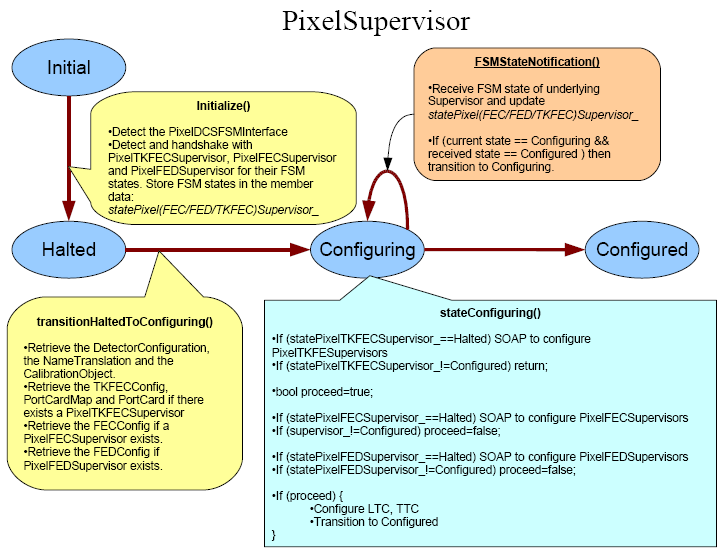
\includegraphics[width=160mm]{PixelSupervisorDAQDCS.png}
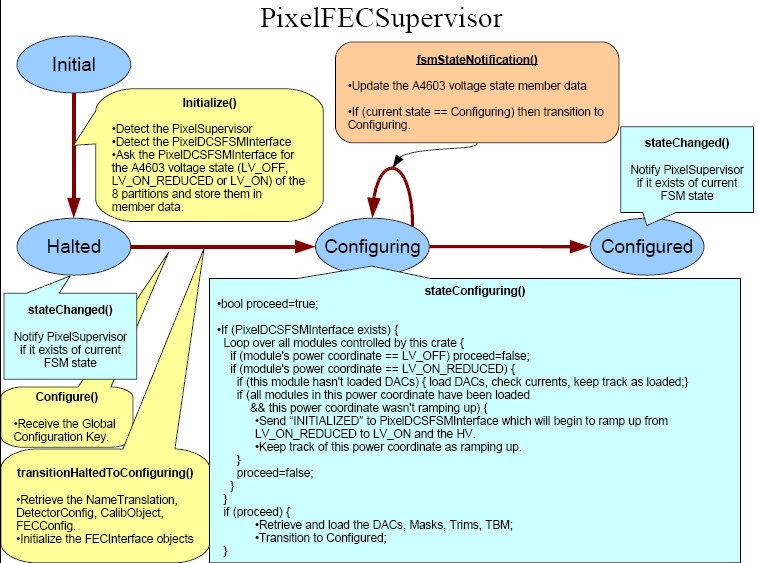
\includegraphics[width=160mm]{PixelFECSupervisorDAQDCS.png}
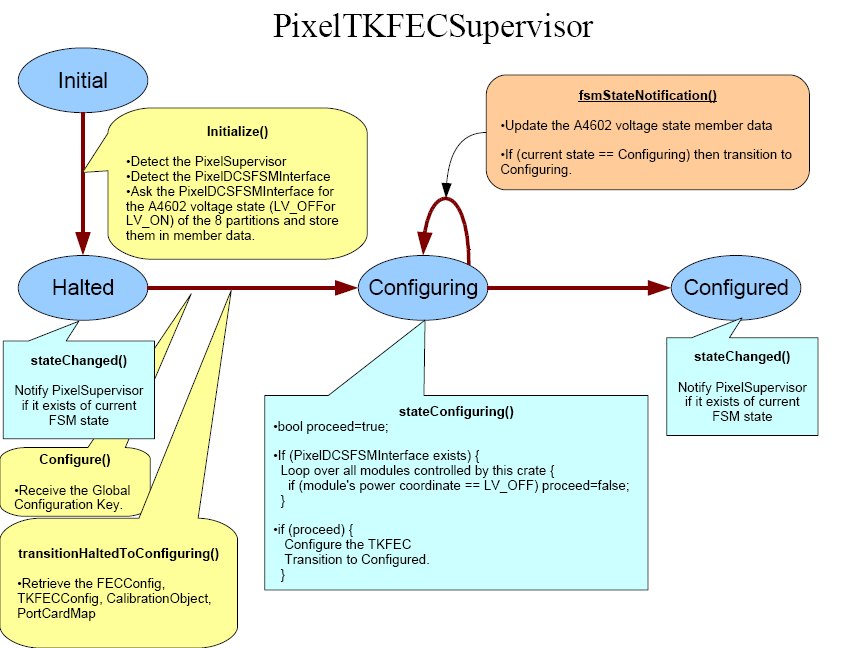
\includegraphics[width=160mm]{PixelTKFECSupervisorDAQDCS.png}
\end{center}

\begin{enumerate}
\item PixelFECSupervisor(s) and PixelTKFECSupervisor are initially
      in their "Initial" state and await the "Initialize" command.

\item On receiving the "Initialize" command, PixelFECSupervisor(s) and
      PixelTKFECSupervisor independently query PixelDCSFSMInterface.% with
%%%%i think this is too much detail
%      the SOAP messages:
%      \begin{verbatim}
%<fsmStateRequest name="PixelFECSupervisor" type="PxlFEC" instance="1">
%</fsmStateRequest>
%
%<fsmStateRequest name="PixelTKFECSupervisor" type="TrkFEC" instance="1">
%</fsmStateRequest>
%      \end{verbatim}
%
%respectively.

\item The PixelDCSFSMInterface responds with information regarding
      the voltage states.% with a SOAP message of the form:
%      \begin{verbatim}
%<fsmStateResponse>
%  <state partition="FPix_BmI">LV_ON;HV_ON</state>
%  <state partition="BPix_BpO">LV_ON;HV_OFF</state>
%  ...
%</fsmStateResponse>
%      \end{verbatim}

Note that in practice, the correct power state is never reported in
the ``Initialize'' step, because at P5 the ``Initialize'' transition
is always triggered immediately after starting the software, at which
point the PixelDCSFSMInterface has not yet had time to make
connections with the PSX server and be notified of the state of the
power supplies. Once the PSX server connections are made,
the correct power state is sent via the standard asynchronous
mechanism.


\item The PixelFECSupervisor(s) and PixelTKFECSupervisor update
      their tri- and bi-state member data (for LV and HV as appropriate)
      according to the response from PixelDCSFSMInterface. This
      concludes the "Initializing" transition
      and both the PixelFECSupervisor(s) and PixelTKFECSupervisors
      land in their "Halted" states.

\item On receiving the "Configure" command, PixelFECSupervisor(s)
      and PixelTKFECSupervisor
      check the status of their member data. If the appropriate
      voltages are set then they go ahead
      with step \ref{item:FECconfig}. If the LV\_OFF state is found, configuration does not proceed.

\item \label{item:FECconfig}
If the PixelFECSupervisor finds that the LV is in state
LV\_ON\_REDUCED, the ROCs' DAC settings are loaded and programmed to
the ROCs. (It has been proposed to query the low-voltage currents
before and after this loading of DAC settings, in order to ensure that
the currents change when the DAC settings are loaded. However this
check is not implemented at present.) If the LV is already in state
LV\_ON (as is the case for the BPix, or on subsequent configurations
of the FPix), this step is skipped.

\item PixelFECSupervisor sends a SOAP message to PixelDCSFSMInterface to notify it that the FPix DAC settings have been loaded. The PixelDCSFSMInterface forwards this message to DCS via the PSX server.
%      The PixelDCSFSMInterface responds back with the raised values of the Digital Voltages.
%      PixelFECSupervisor resets its
%      tristate member data if this went fine or else
%      transitions to its "Error" state.

%\begin{verbatim}
%<fsmStateNotification>
%  <state partition="FPix_BmI">INITIALIZED</state>
%  <state partition="BPix_BpO">INITIALIZED</state>
%</fsmStateNotification>
%\end{verbatim}

\item PixelFECSupervisors wait for an LV\_ON SOAP message from PixelDCSFSMInterface.

\item PixelFECSupervisors load their ROCs' DAC, mask and trim settings. When
programming the DACs, we check the state of the data member containing
the HV status.  The PixelTKFECSupervisors load the slow I2C
settings for CCU boards, Port Cards etc.

\item The PixelFECSupervisor(s) and PixelTKFECSupervisor(s) land in
      their "Configured" state.

\end{enumerate}

During the configure step in PixelFECSupervisor, we follow the
``HV-dependent'' DAC programming procedure if and only if we are
configuring for a calibration. If we are configuring for Physics
running, then the ROCs are always disabled (treated as if the HV was
off).

\subsection{HV-dependent DAC programming}

At Configure (for calibrations only), and at the Start and Resume
transitions, we check the data members that store the HV status, and
we check the data members that track whether the ROCs were most
recently enabled or disabled. If we find that the HV is on and the
ROCs were previously disabled, we enable the ROCs. If we find that the
HV is off and the ROCs were previously enabled, then we disable the
ROCs. If we HV is on but the ROCs are already enabled, then we do
nothing; similarly if the HV is off but the ROCs are already disabled.

To disable the ROCs, we overwrite the VcThr DAC setting with 0
(high threshold), then disable the ROCs using the ROC control
register. These procedures are implemented in the PixelDACSettings
class. This class caches the DAC settings from the DB, and if we
override the VcThr setting with zero we do not change what is in the
cache, so no new DB accesses are needed when we want to enable the ROCs. The
PixelDACSettings::generateConfiguration() method has an argument for
the calling function in PixelFECSupervisor to indicate the status of
the HV. To enable the ROCs, the nominal VcThr and CCR settings are programmed.

%comment from Anders:
%For the PixelFECSupervisor to read out the current I suggest that
%this is done by calling the PixelSupervisor. The PixelSupervisor
%will have all the configuration information needed to read the
%currents.

\subsection{Start and Resume transitions}
The status of the HV is checked and the DACs are programmed if needed, as explained above.

\subsection{Pause, Stop, and Halt transitions}
The ROCs are disabled as if the HV was off.


\subsection{Expected behavior}
As currently implemented, the following is the expected sequence of events when turning on the FPix:
\begin{itemize}
\item User turns FPix to ON in DCS
\item FPix is powered to LV\_ON\_REDUCED (called DIGITAL\_ON\_REDUCED in DCS)
\item User begins the Configure transition in PixelSupervisor
\item FPix DACs are programmed
\item POS notifies DCS that the DACs are programmed; POS then waits in the ``Configuring'' state
\item DCS raises the digital voltage to the nominal value
\item POS is notified that we have reached the LV\_ON state
\item DCS begins to ramp the high voltage.
\item Configuration in POS proceeds with the reprogramming of the DACs and the programming of the trims and masks
\item Configuration in POS finishes. At some point (probably after the end of configuration), the high voltage reaches its nominal value and DCS notifies POS that we have reached the HV\_ON state (called simply ON in DCS).
\item Because the HV was not on at the time of configuration, the DACs are set to the special settings used for HV\_OFF
\item User presses Start to begin a calibration in POS
\item The FEC Supervisor notices that the state of the HV has changed since the configuration. Therefore the VcThr and chip control register DACs are set to their nominal values. Because of this settings change, the user will see a large change in the amount of digital current drawn by the FPix.
\item The calibration proceeds as normal.
\end{itemize}

\subsection{Notes on hardcoding of information} \label{sec:dcshardcode}

Because the XDAQ software (POS) and DCS use different naming schemes
and different granularity, several translations must be made in order
for POS to communicate with DCS. Some of these translations are
encoded in the {\tt interface.xml} file, while others are hard-coded
in the logic of the PixelDCSFSMInterface.

Specifically, the xml file defines which ROGs\footnote{readout
groups} exist, and which PVSS datapoint name belongs to which
ROG\footnote{These datapoints are used to indicate when POS has
configured the ROCs on a ROG.}. The xml file also defines the POS
applications that need to be notified in case the state of a ROG
changes.

The hardcoded logic in PixelDCSFSMInterface defines which ROG
correponds to which pieces of the detector (which ROCs are supplied by
which power supply).

In principle, this information could be instead contained in a database table with roughly 5 fields:


\begin{tabular}{ll}
Field in database & Example value \\
\hline
POS name          & FPix\_BmI\_D2\_BLD1 \\
DCS name          & {\tiny CMS\_TRACKER:PixelEndCap:PixelEndCap\_BmI:PixelEndCap\_BmI\_D2:PixelEndCap\_BmI\_D2\_ROG1} \\
datapoint name    & {\tiny cms\_trk\_dcs\_10:tkPg\_CAEN \textbackslash CMS\_TRACKER\_SY1527\_5 \textbackslash branchController05 \textbackslash easyCrate3 \ldots} \\
%{\tiny cms\_trk\_dcs\_10:tkPg\_CAEN \textbackslash CMS\_TRACKER\_SY1527\_5 \textbackslash branchController05 \textbackslash easyCrate3 \textbackslash easyBoard04.pixelSequence.configured} \\
SOAP connection (TKFEC) & PixelTKFECSupervisor instance 2 \\
SOAP connection (FEC) & PixelFECSupervisor instance 2 \\
\hline
\end{tabular}


With a table such as this, we could eliminate both the xml file and the hardcoding.

\section{Procedures to follow when hardware components are replaced}

This section documents the procedures that are to be followed
when off detector hardware components are replaced that
affects the online software and calibrations.

\subsection{FED board}

As the FED decodes the analog levels it will be required to
redo several calibrations to check the optical connections
after replacing a FED. The FED firmware version has to
be validated.
The following calibrations should be run
\begin{itemize}
\item FED baseline
\item AOH gain
\item AOH bias
\item FED baseline (it is possible that the previous three steps
          has to be repeated.)
\item FEC clock and phase
\item TBM UB
\item ROC UB
\item Address level
\end{itemize}

\subsection{Pixel FEC including mFECs}

 No calibrations should be affected by replacing a FEC board
or a mFEC --- in principle. However, we have seen that the
size of the window for good communication changes a little
between different mFECs. This seems mostly to affect the
return data and this check is now disabled for both FPix
and BPix. It is probably prudent to rerun a Delay25 calibration
to check that after reconnecting the fibers we have the expected
performance.

Need to verify that the right firmware is installed. I assume
that we manage to connect the fibers in the right slot.

\subsection{TKFEC}

 No calibrations should be affected by replacing a TKFEC board.

Need to verify that the right firmware is installed. I assume
that we manage to connect the fibers in the right slot.

\section{Low-level commands}

In addition to the complex sequences of commands issued by the
high-level configuration procedure, a number of low-level commands are
available to the user through the GUIs of the various
Supervisors. These can be useful for expert-level problem
solving. These are described in this section.

\subsection{Resets}

\begin{itemize}
\item ResetROC: sent via the TTC. Availabe as a button in the PixelSupervisor GUI. Implemented and verified to work.
\item ResetTBM: sent via the TTC. Availabe as a button in the PixelSupervisor GUI. Implemented and verified to work.
\item ResetCCU: causes the TKFECSupervisors to issue the command {\tt resetPlxFec()}. Availabe as a button in the PixelSupervisor GUI. Implemented. Sends resetPlxFec via the FecSoftware.
\item PIA resets: a menu of resets available from the PixelTKFECSupervisor GUI, implemented by passing a value to the FecSoftware command {\tt testPIAResetfunctions}
\begin{itemize}
\item roc: value = 0x1
\item aoh: value = 0x2
\item doh: value = 0x4
\item res1: value = 0x8
\item res2: value = 0x10
\item fpixroc: value = 0x2A (bits 1, 3, and 5); this resets the TBM and ROCs
\item fpixdevice: value = 0x15 (bits 0, 2, and 4); this resets the portcard devices (Delay25, DOH, AOH, DCU)
\end{itemize}
The PIA resets are hard resets using hardware lines. In the FPix they go from the CCU parallel output lines to reset lines on the portcard. One is fanned out to all the portcard devices. The other is routed to the TBM and ROCs through the adapter board\footnote{https://hypernews.cern.ch/HyperNews/CMS/get/pixelOnlineSW/1155/1/1.html}.
\end{itemize}



\clearpage

\appendix
\section{FED phase and delay calibration}
\label{sect:phaseanddelay}

This section will describe some aspects of determining the
so called `phase' and `delay' of the FED. The sample
plots shown in this section are taken from runs on the
FPIX pilot run detector. This was done using a version 4 FED
with the Aug. 22, 2007 firmware version.

In order to get the transparent data to 'look' OK I had
to send an LRES before each trigger. I think
that the final conclusion was that the FED state machine
gets confused when the input data is non standard. In the
scans over phases and delays there are certain settings that
are invalid, i.e., that you try to read out the ADC before the
data is available. At the end of this section I will discuss
two issues that I noticed in looking at the transparent data.

For the above reason we also turn off the automatic baseline
correction to avoid it getting confused if you send non valid
data or if you don't have correct address levels.

In these tests we take 10 triggers for each delay and phase
setting. I'll show plots, as in Fig.~\ref{fig:phasedelayraw},
where for each of the two possible phases the profile
histogram shows the adc value as a function of clock+delay/16.
The third plots just show the two plots on top of each other.
\begin{figure}
\begin{center}
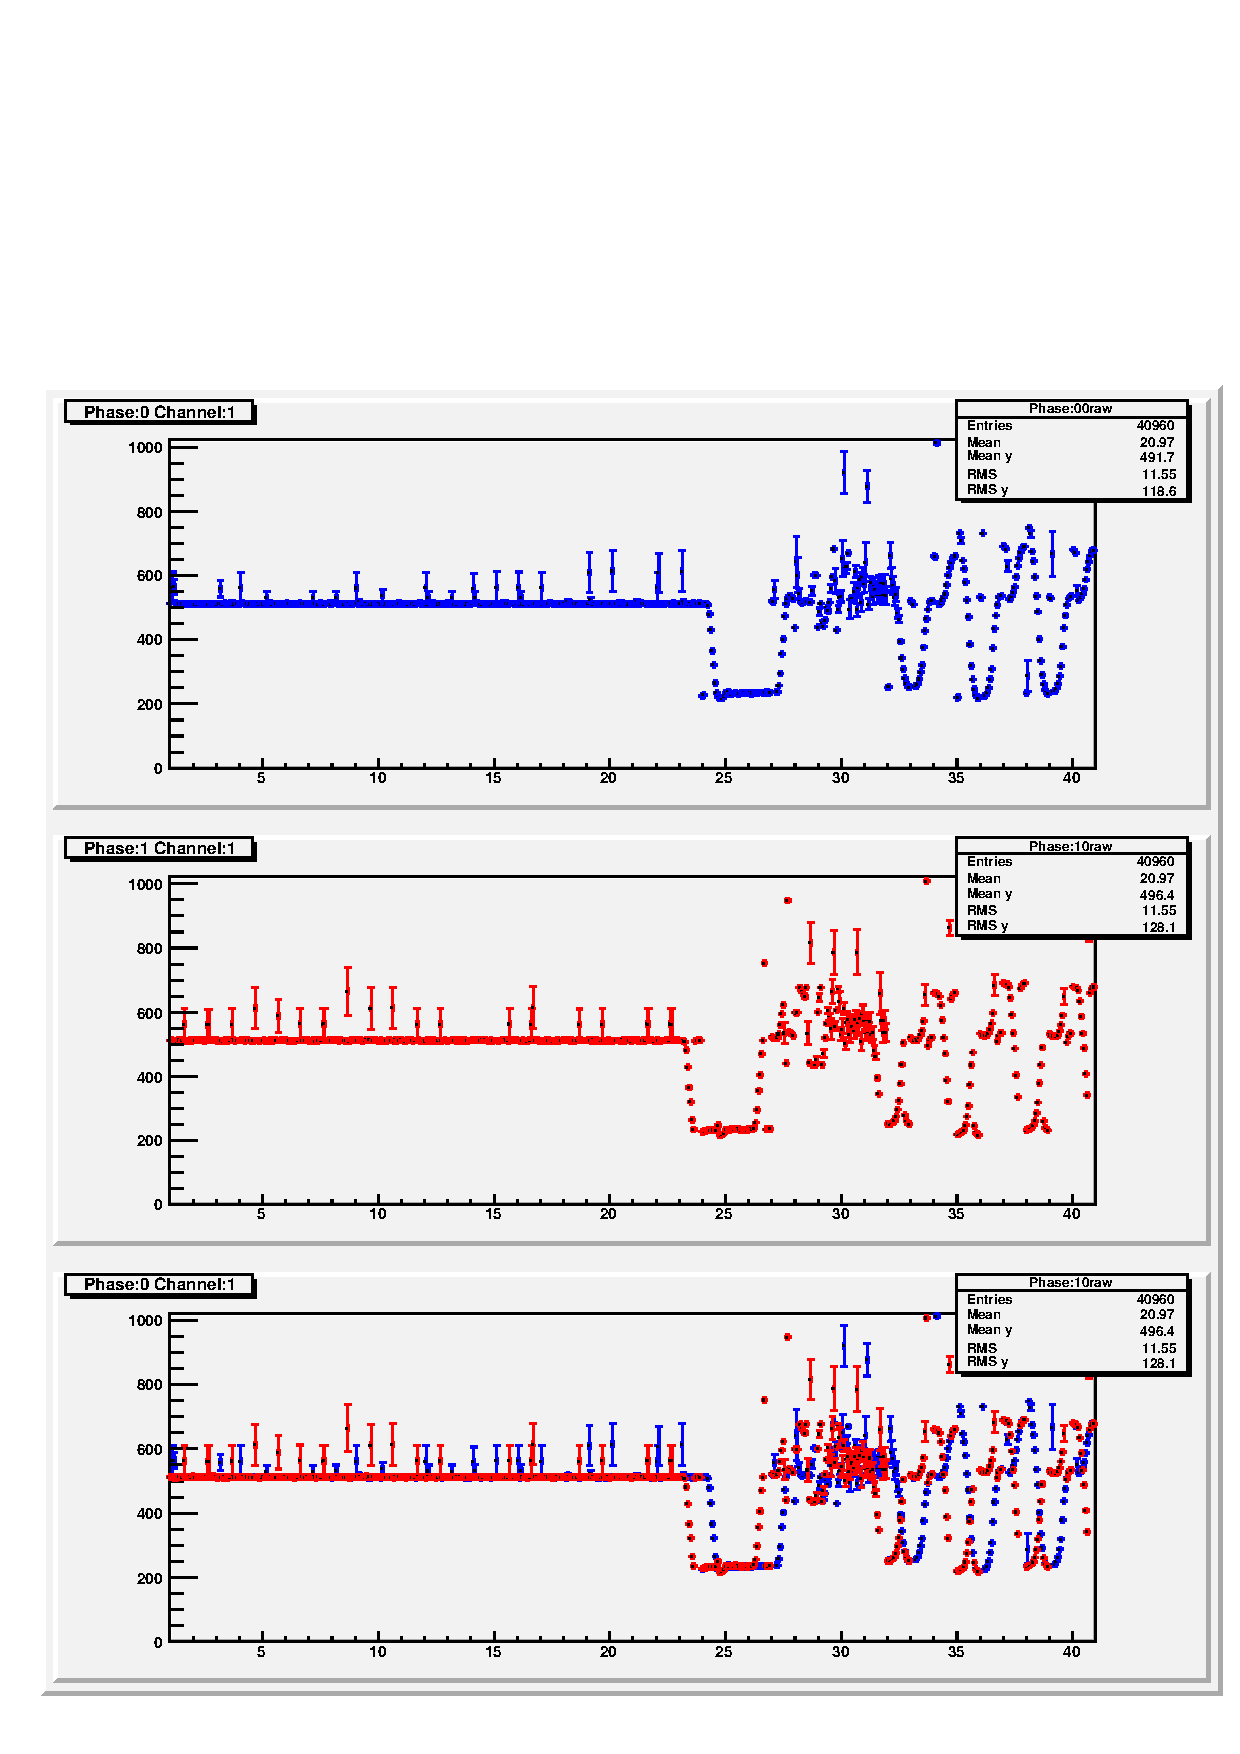
\includegraphics[width=\linewidth]{phaseAndDelayPlotRaw_channe_1_1}
\end{center}
\caption{This figure shows on top the adc value as a function of
clock+delay/16 for phase=0 and the same plot for phase=1 in the
middle. The two plots are overlaid at the bottom.}
\label{fig:phasedelayraw}
\end{figure}
We see that
there are certain values of the delays that produce garbage
as you try to read out the ADC before the data is available.
To identify the invalid combinations of phase and delay I
calculate the rms for the different phase and delay settings
in the first 20 clock cycles, i.e. before the TBM header arrives.
Based on the rms distribution it is seen that for phase=0
we got invalid data with delays of 1, 2, and 3, while for
phase=1 the delays of 10, 11, and 12 generate invalid data.
From now on I will reject these combinations. (In the plots I set the
adc value to 0.)

After rejecting the invalid phase and delay combinations we now
have a signal that looks as what is shown in Fig.~\ref{fig:phasedelayvalid}.
\begin{figure}
\begin{center}
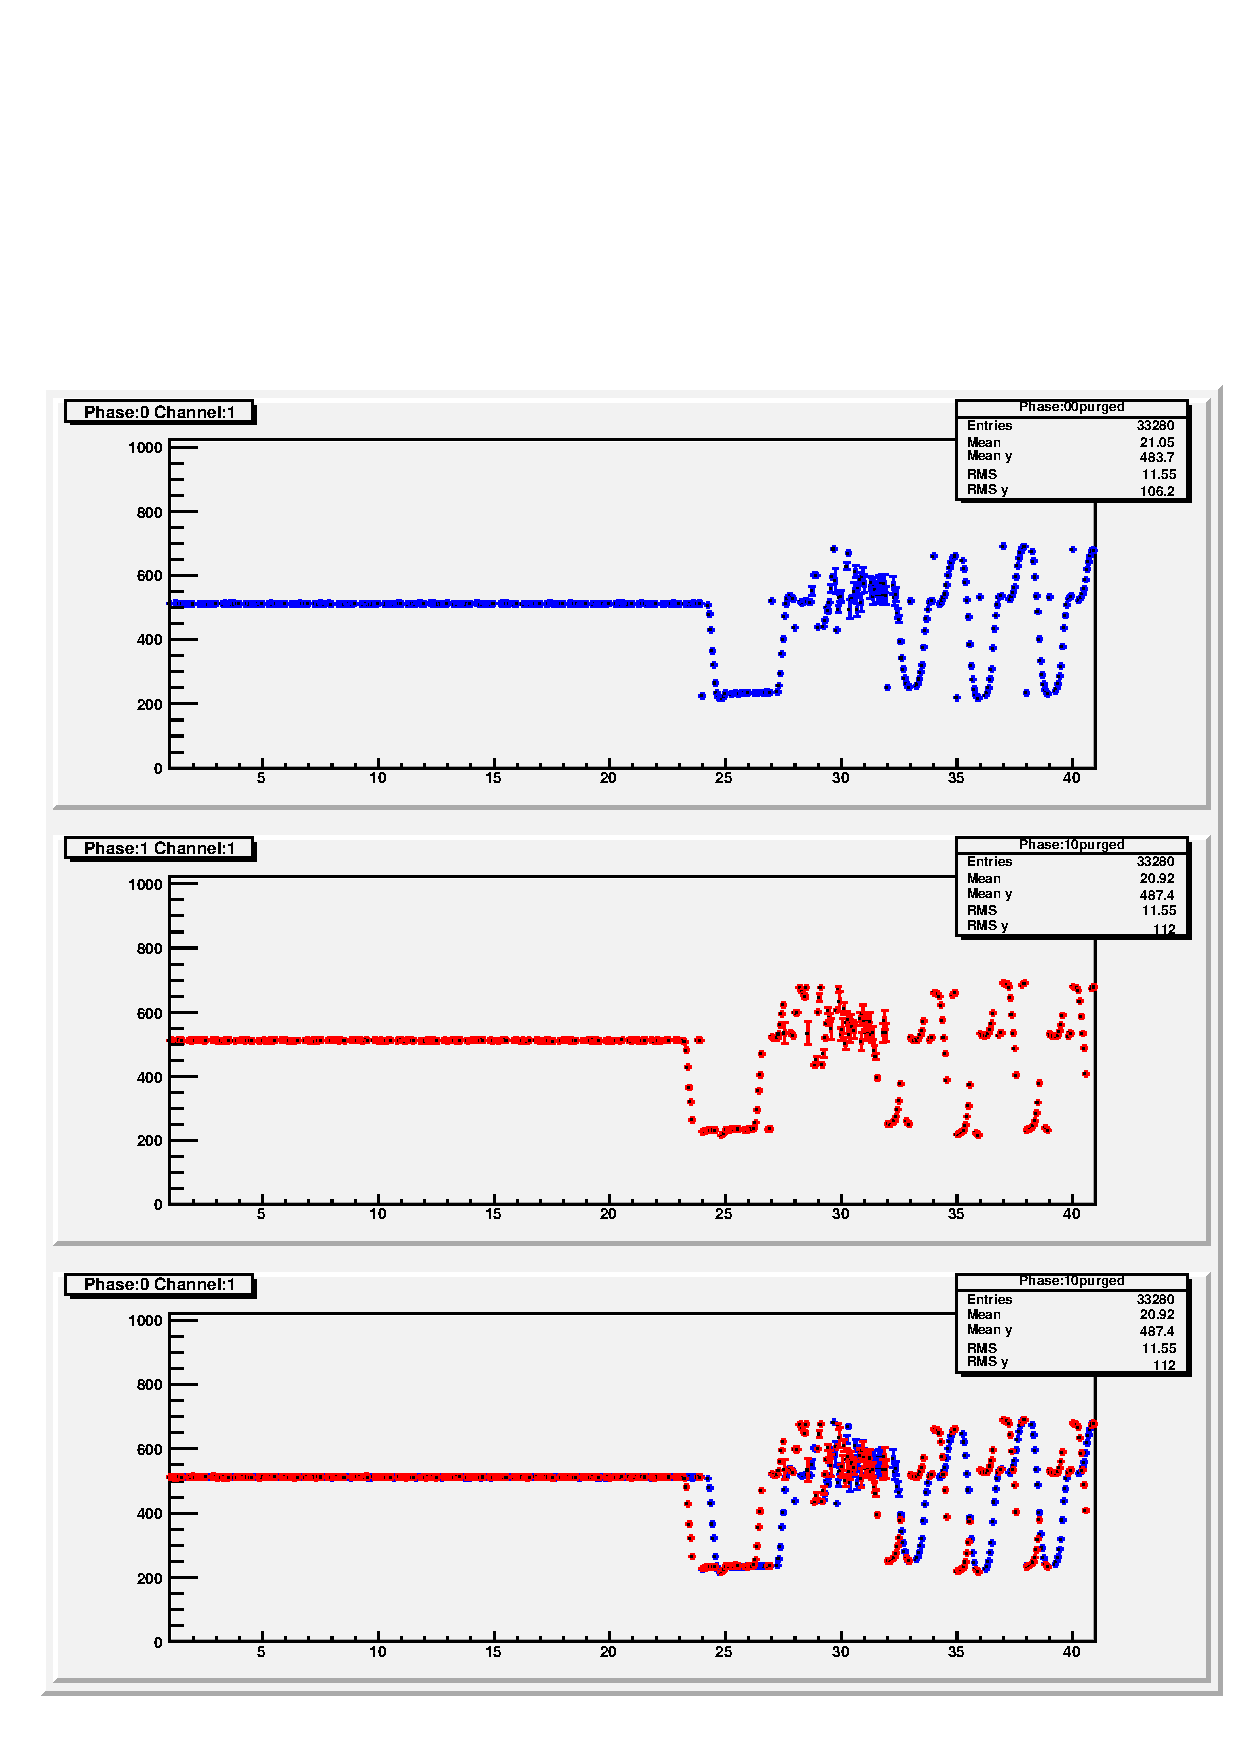
\includegraphics[width=\linewidth]{phaseAndDelayPlotPurged_channe_1_1}
\end{center}
\caption{This figure shows on top the adc value as a function of
clock+delay/16 for phase=0 and the same plot for phase=1 in the
middle. The two plots are overlaid at the bottom. Here I have set the
adc value to 0 for the combinations of clock and phase that are not
valid.}
\label{fig:phasedelayvalid}
\end{figure}
The remaining signal still has artifacts due to when the
adc latches on to the signal such that it looks like the signal
is not read out in order. This is corrected by 'reordering' the data
within a clock. I shifted the phase=0 events backward by 3 delay steps
and the phase 1 events forward by 3 delay steps. This makes the
signal continuous as shown in Fig.~\ref{fig:phasedelayshifted}.
\begin{figure}
\begin{center}
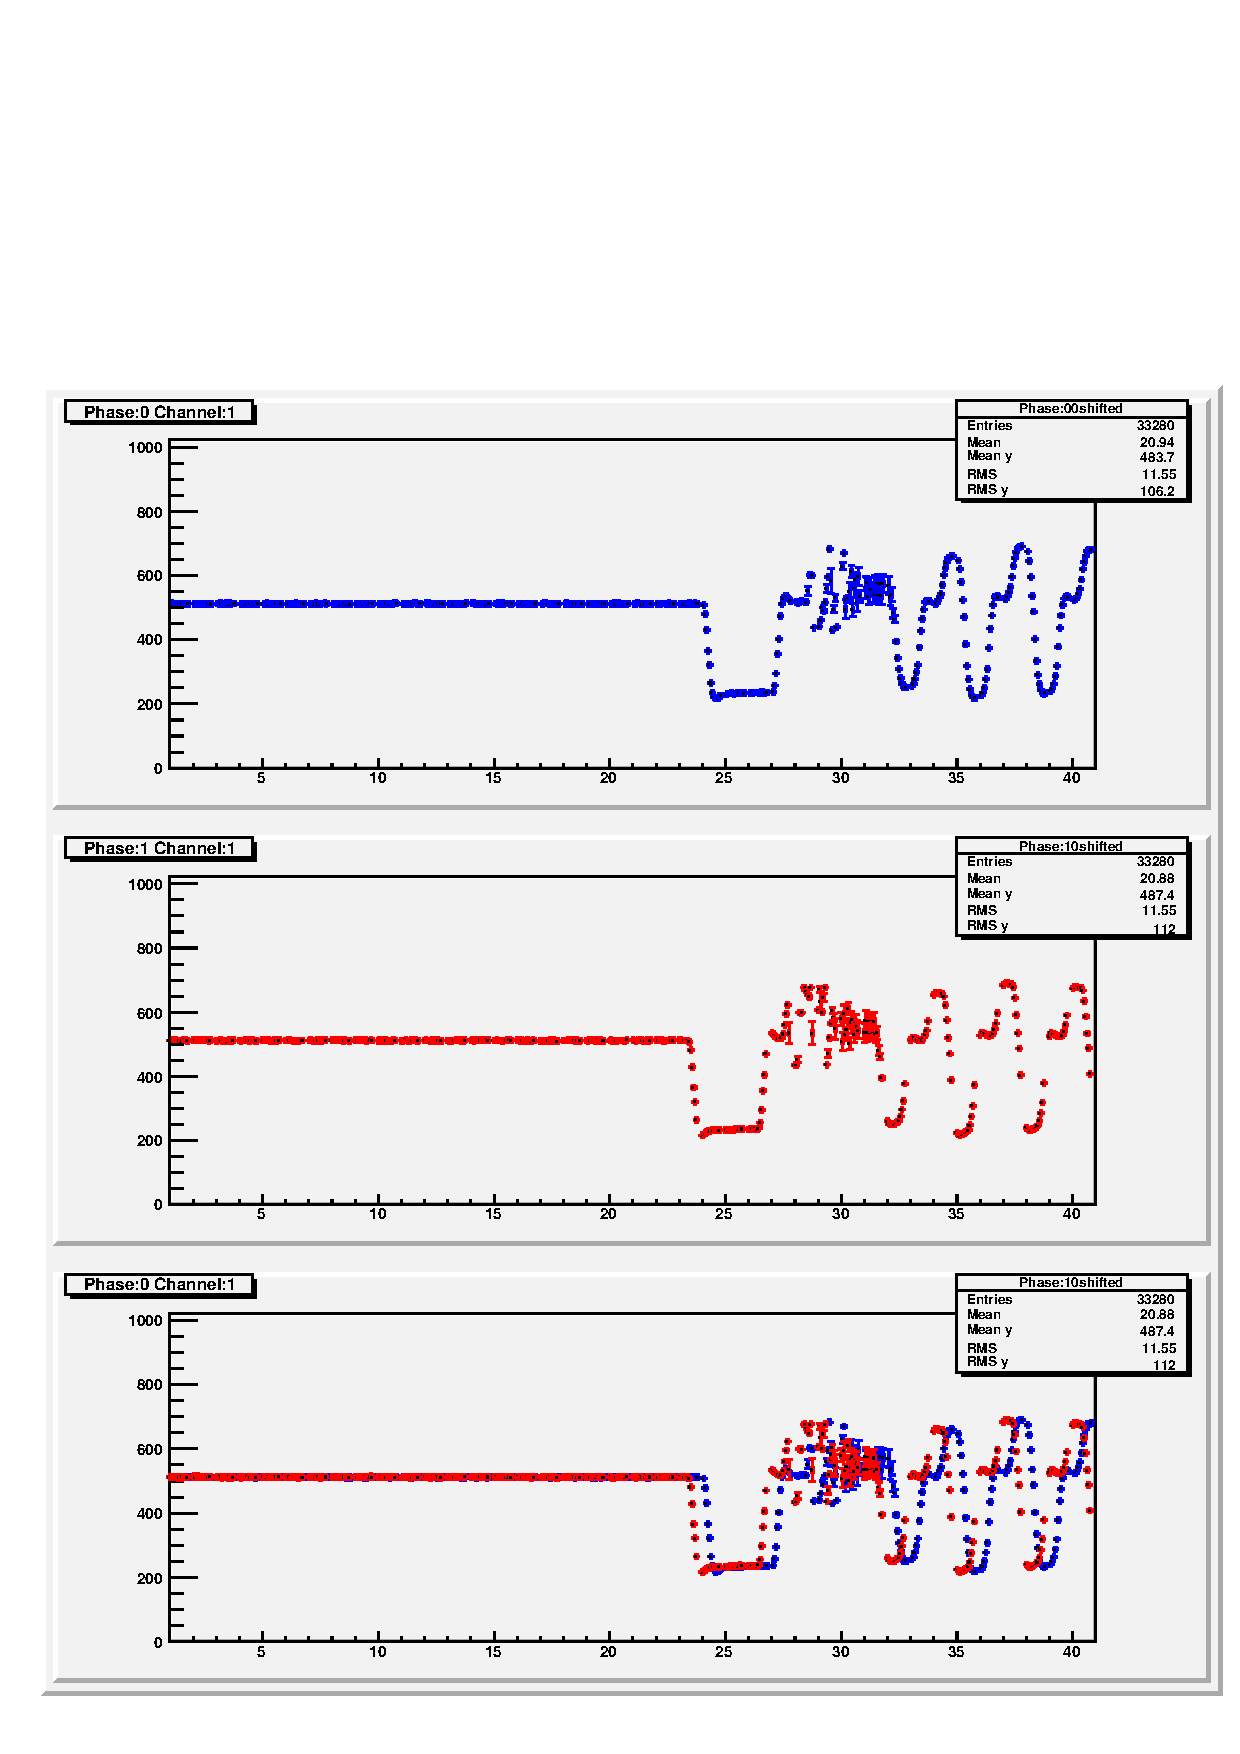
\includegraphics[width=\linewidth]{phaseAndDelayPlotShifted_channe_1_1}
\end{center}
\caption{This figure shows on top the adc value as a function of
clock+delay/16 for phase=0 and the same plot for phase=1 in the
middle. The two plots are overlaid at the bottom. Here the
data within a clock has been ordered to give a continuous data
signal.}
\label{fig:phasedelayshifted}
\end{figure}


The last step is to align the data so that the phase=0 and phase=1
data overlaps. I do this by shifting the data for the events with phase=1
by 10 delay steps. The final result is shown in
Fig.~\ref{fig:phasedelayfinal}. For the bins in the plot where there
is data from both phase=0 and phase=1 we see that there is excellent
agreement. We also note that the signal undershoots in a transition
from black to ultrablack and that it overshoots on the reverse transition.
\begin{figure}
\begin{center}
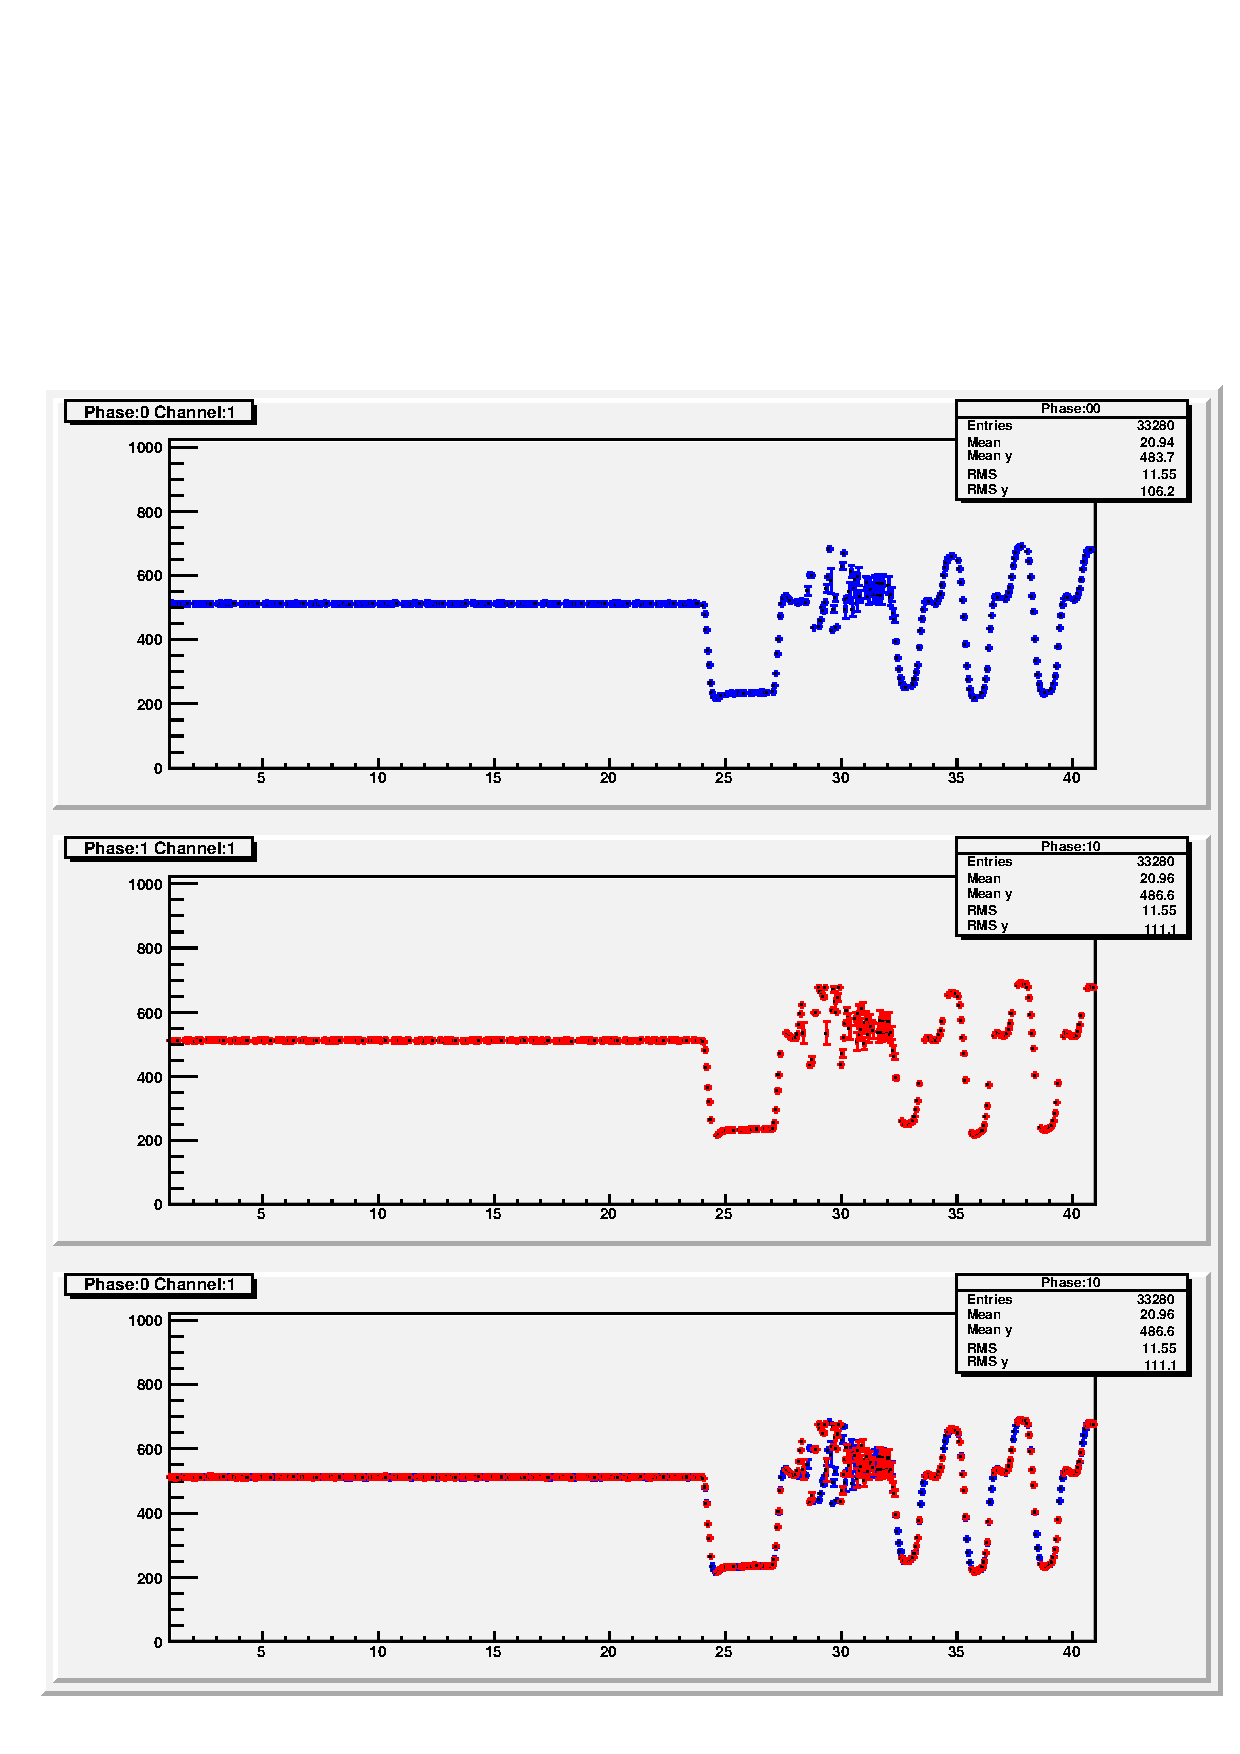
\includegraphics[width=\linewidth]{phaseAndDelayPlot_channe_1_1}
\end{center}
\caption{This figure shows on top the adc value as a function of
clock+delay/16 for phase=0 and the same plot for phase=1 in the
middle. The two plots are overlaid at the bottom. Here the phase=1
data has been shifted so that it overlaps with the phase=0 data.}
\label{fig:phasedelayfinal}
\end{figure}


To determine a best delay I look at the combined data - where I average
the bins that has both phase=0 and phase=1 contributions - and calculate
a difference for bin $i$ by taking the difference between bin $i-1$
and $i+1$.
I calculate this difference for the 25 MHz clock cycles from clock 27 to 100.
I add the magnitude of these differences for all bins that corresponds
to the same delay. I pick the smallest such sum of differences for the
different delay as the optimal choice. If more than one phase is allowed
I pick the choice that is farthest from the invalid delay for that phase.

A new alogorithm has been implmented that determines the phase
to be right at the edge of the transition from black to ultrablack
in the TBM trailer. You can still run the old algorithm by setting
the parameter 'oldMode' to 'Yes'.


Looking at the 8 channels that were connected to the pilot run detector
I find that the results are very consistent. The phase is either 0 or
15 in the (aligned delay) for the raw delay setting this corresponds
to 2 or 3 for phase=1.

%Open questions: Is the same set of phases and delays illegal on all
%FEDs and channels? Also, are the shifts that are needed to time-order
%the data the same on all FEDs and channels? Looking at more data will
%resolve this. It is easy to test that the data in the two phases are
%compatible by forming a $\chi^2$.

The code was written as a root macro. I will 'transplant' this code
into XDAQ so we can run it automatically to produce the phase and delay
settings needed.

However, looking at this I observed an odd feature.
This is illustrated in Fig.~\ref{fig:phasedelaylatedata}.
\begin{figure}
\begin{center}
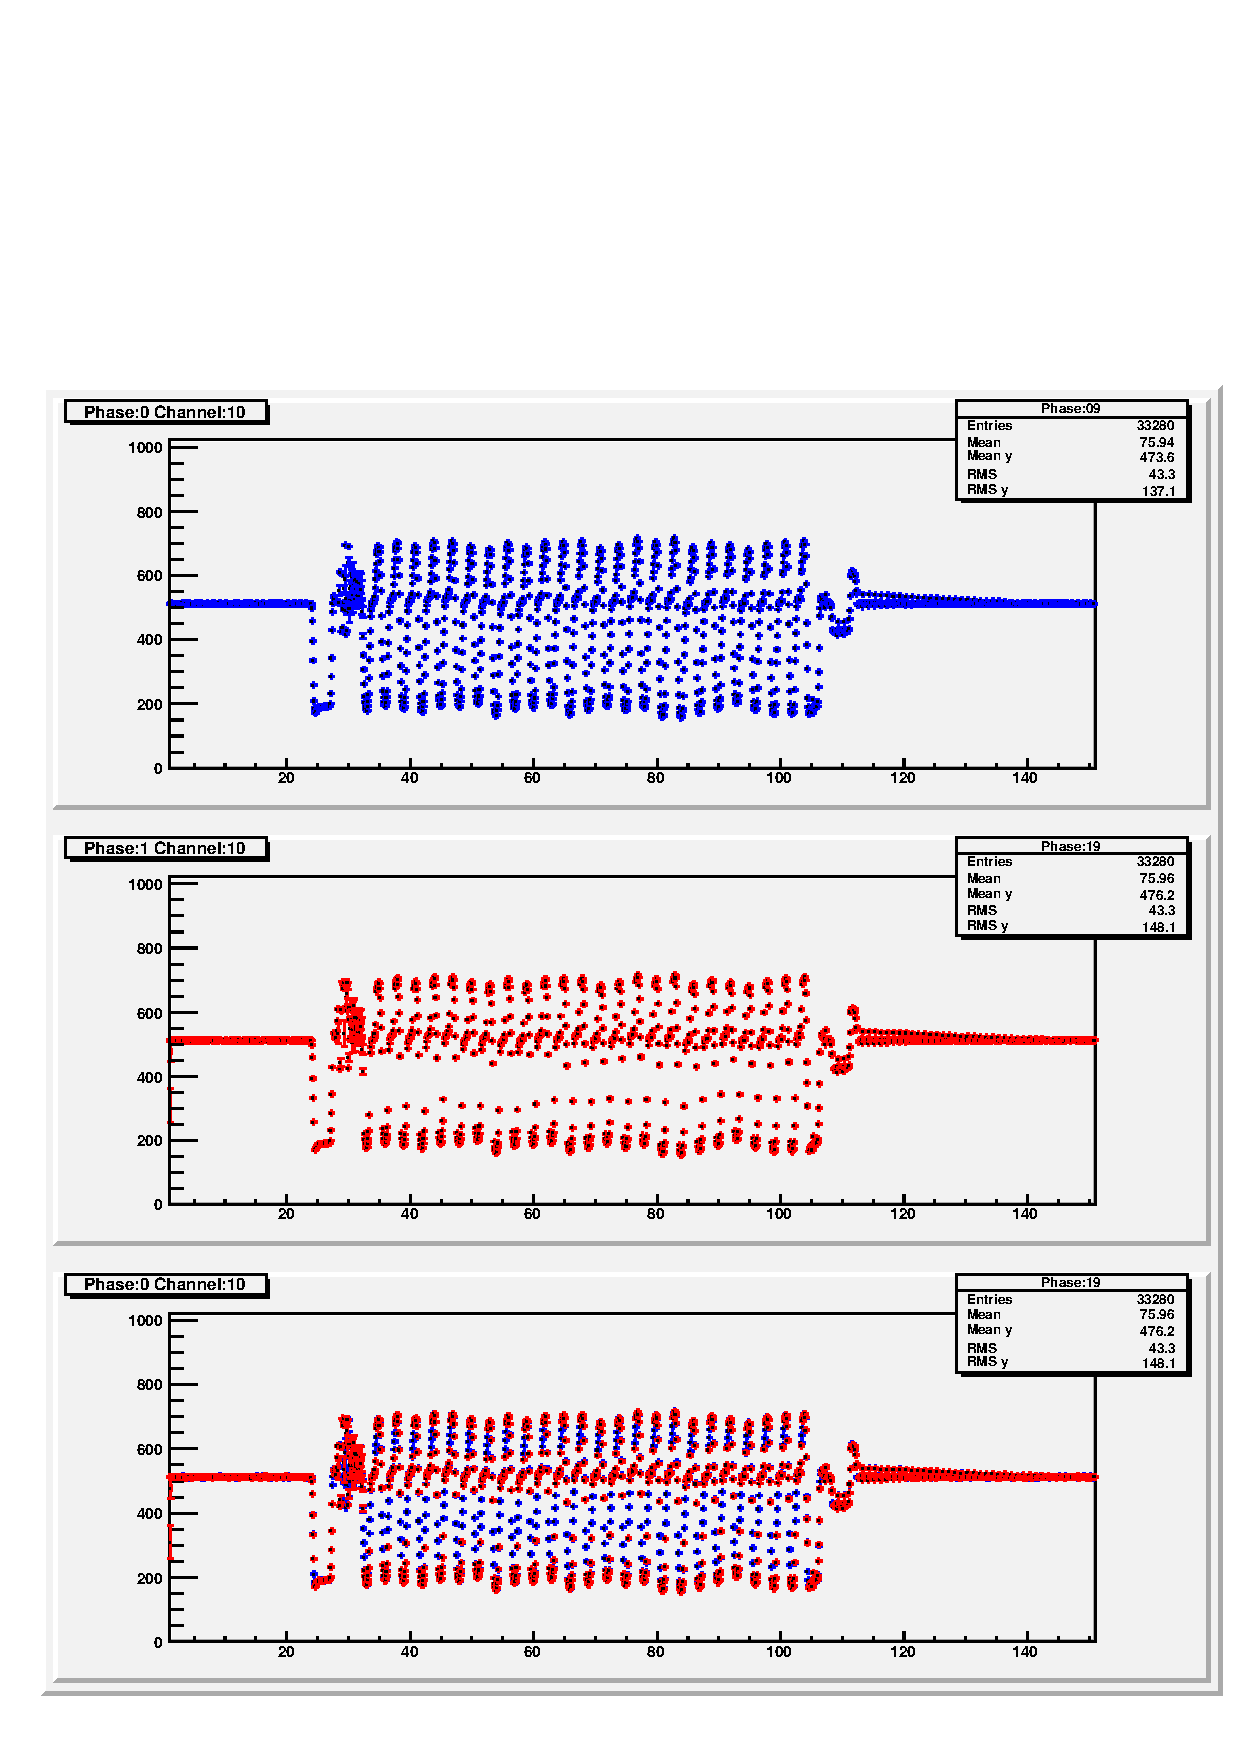
\includegraphics[width=\linewidth]{phaseAndDelayPlot_channe_10_1_latedata}
\end{center}
\caption{Here you see that for clocks in and after the TBM trailer that
there is a feature in that some delays are oscillating. This 'excitation'
seems to decay of after $O(20)$ clocks. }
\label{fig:phasedelaylatedata}
\end{figure}
In Fig.~\ref{fig:phasedelaylatedatazoom} is a close up of the
region with the noise.
\begin{figure}
\begin{center}
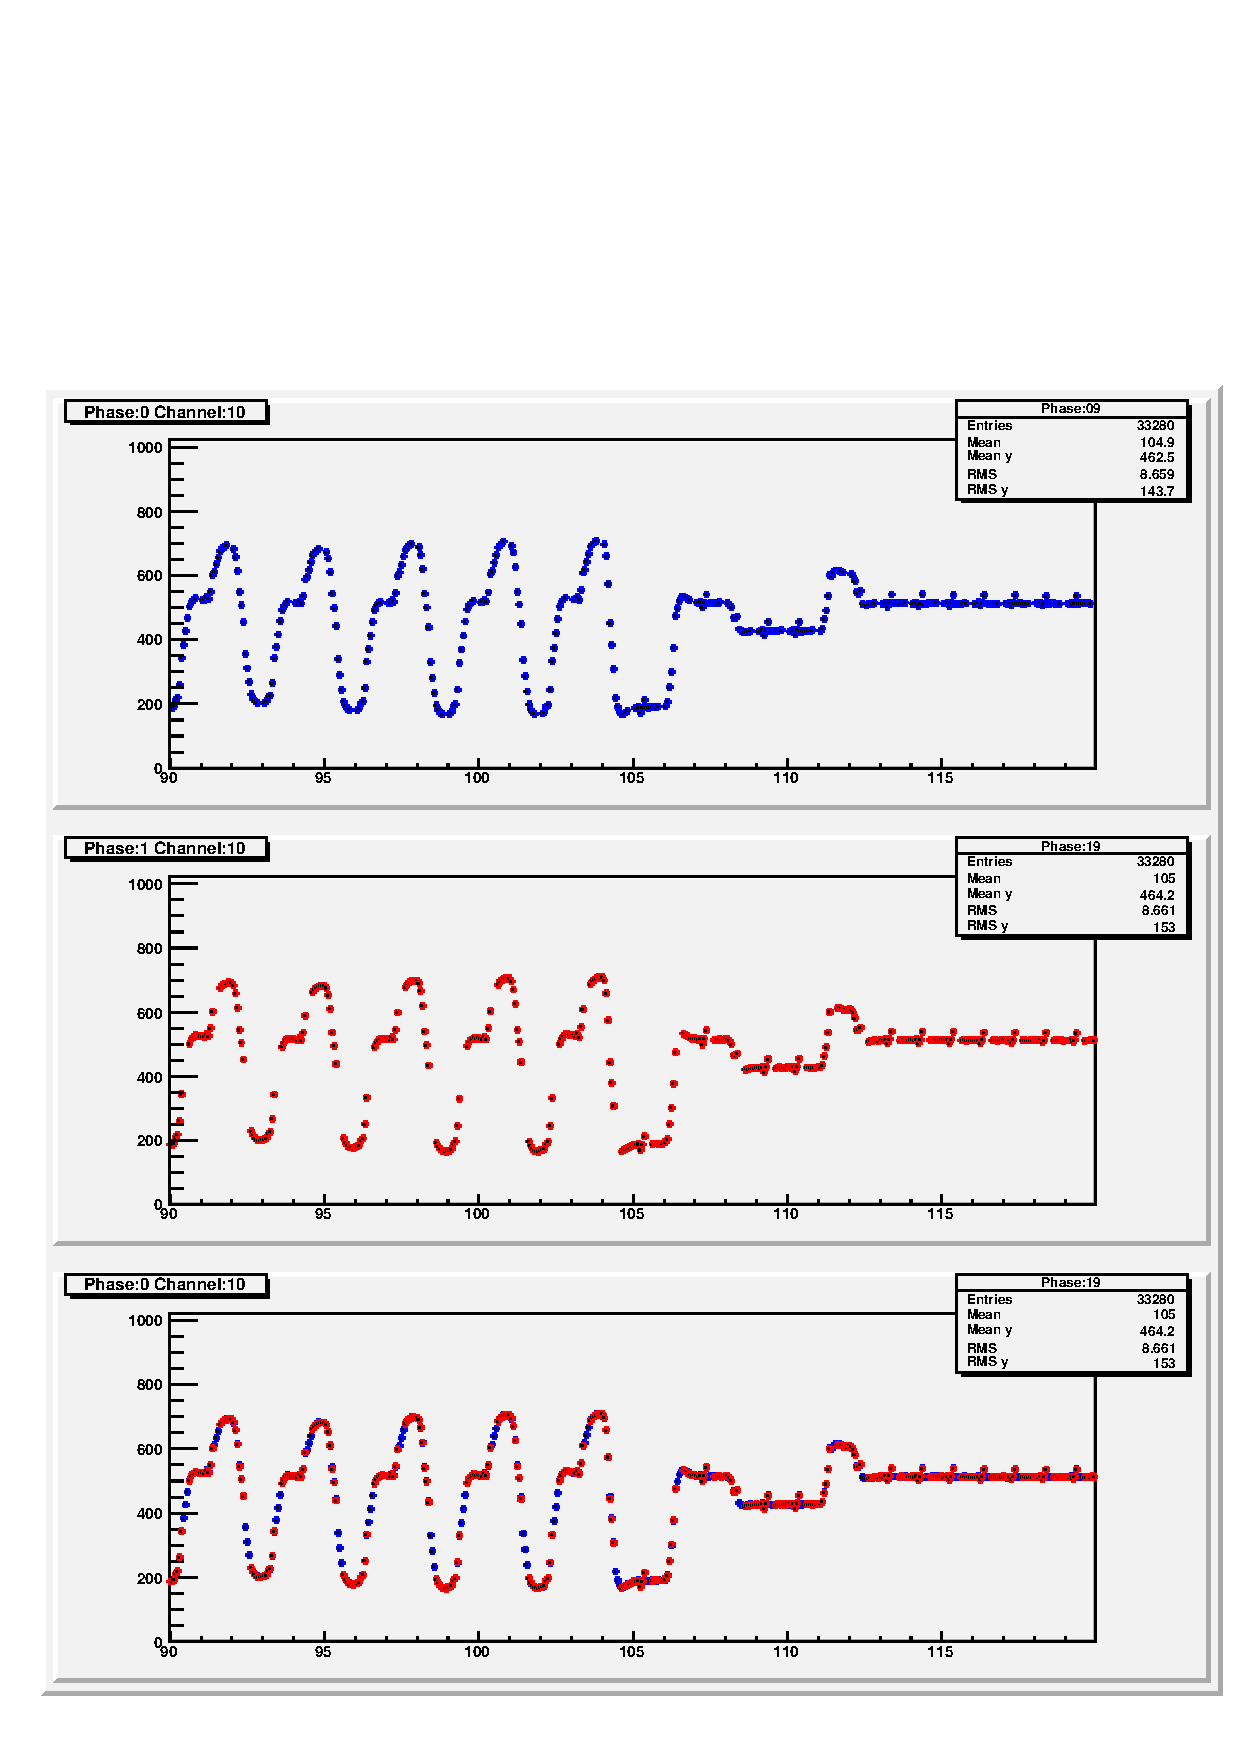
\includegraphics[width=\linewidth]{phaseAndDelayPlot_channe_10_1_latedatazoom}
\end{center}
\caption{Zooming in you can see that data in the two phases
both agree on the shape of this feature. }
\label{fig:phasedelaylatedatazoom}
\end{figure}
Here you can see that there is 'wiggle' in the data that is large compared
to the rms, as indicated by the error. This wiggle seems to persist
for many clock cycles after the TBM trailer. However, it was not present
in the black data before the data train. It seems to first start
in the TBM trailer when the UB signal is generated. With the
pilot run detector we are using 8 channels
(1, 2, 3, 4, 7, 8, 9, and 10). I see the same feature on
almost all channels, though they are not as strong on channel 1, 7,
and 9.


\section{Calibration Organization}

The calibrations all share a similar format.
\begin{itemize}
\item The PixelSupervisor controls a loop over 'events' and coordinates
      the activity of the FED, FEC, TKFEC, and TTC supervisors.
\item Each calibration needs to do some initialization before processing
      the event data.
\item During event processing data is acquired and processed.
\item After all event data is taken it is analyzed and the results are
      saved.
\end{itemize}
This section will describe a proposal for how to formalize this process.
A first step in this direction was taken when the calibration classes
were broken out from the PixelSupervisor and the PixelFEDSupervisor.
This first step was almost trivial as it just copied the code out to
separate classes. There are a few more changes we should make that will
allow us to run these jobs in workloops. Among other things, this will
allow us to look
at the progress of the calibrations from the web browser.

\subsection{PixelSupervisor calibration code}

We change the {\tt PixelCalibrationBase} class to have
the interface below.
\begin{verbatim}
class PixelCalibrationBase : public PixelSupervisorConfiguration,
	    public SOAPCommander {
 public:

  PixelCalibrationBase( const PixelSupervisorConfiguration &,
			   const SOAPCommander& soapCommander  );

  virtual ~PixelCalibrationBase(){};

  virtual void beginCalibration();

  virtual bool calibrationEvent();

  virtual void endCalibration();

 protected:

  private:

  // PixelCalibrationBase Constructor
  PixelCalibrationBase(const SOAPCommander& soapCommander);

};
\end{verbatim}

The method {\tt begin()} should do any initialization that
is needed before processing any triggers. The method {\tt event()}
is called repeatedly until it returns true, this indicates that
the calibration has come to an end.
Then the {\tt end()}
method is invoked to perform any analysis of the acquired data.


More details on what these methods need to do will be
discussed below.


\subsection{PixelFEDSupervisor calibration code}

Similarly, I suggest a more general structure for the calibration
code that runs in the PixelFEDSupervisor.

\begin{verbatim}
class PixelFEDCalibrationBase : public PixelFEDSupervisorConfiguration,
	    public SOAPCommander {
 public:

  PixelFEDCalibrationBase( const PixelFEDSupervisorConfiguration &,
			   const SOAPCommander& soapCommander );

  virtual ~PixelFEDCalibrationBase(){};

  virtual xoap::MessageReference beginCalibration(xoap::MessageReference msg);

  virtual xoap::MessageReference calibrationEvent(xoap::MessageReference msg);

  virtual xoap::MessageReference endCalibration(xoap::MessageReference msg);

  //Should really not be here....
  unsigned int TransparentDataStart (unsigned long *buffer);


 protected:

  //SOAPCommander* theSOAPCommander_;

 private:

  // PixelCalibrationBase Constructor should neve be called
  PixelFEDCalibrationBase(const SOAPCommander& soapCommander);

};
\end{verbatim}

Again the three methods {\tt beginCalibration()},
{\tt calibrationEvent()}, and {\tt endCalibration()}
corresponds to the pre calibration data taking, processing of trigger
and the post data taking analysis respectively. I suggest that
these methods are bound to soap messages that invokes
the implemented methods.

In particular we should move the code that sets the mode
and control registers to the {\tt beginCalibration()} method.
This will allow us to move out code from the PixelFEDSupervisor
that is specific to different calibrations. {\it Or we split
out the mode and control register settings to a new configuration
object.}

\subsection{Implementation of algorithms}

During the configuration step the {\tt PixelSupervisor} and
{\tt PixelFEDSupervisor}
instantiates the Calibration class for the calibration objects.
When we go to Run the PixelSupervisor invokes the {\tt beginCalibration()}
method. This method is responsible for sending the {\tt beginCalibration()}
message to the PixelFEDSupervisors.

After this the PixelSupervisor should execute the {\tt calibrationEvent()}
in a workloop until it has completed. Again, the code executed in the
PixelFEDSupervisor is responsible for calling the appropriate
supervisors. This gives the maximal flexibility in the calibration
algorithm.

Last, the {\tt endCalibration} method in the {\tt PixelSupervisor} is
invoked to complete the analysis of the collected data and report
the results.

In addition it would be nice to take out the code from the PixelSupervisor
and the PixelFEDSupervisor that select the calibration type. One
way of doing this is to create a 'factory' for calibrations in the
PixelCalibrations package. This factory would accept a string from
the calibration mode and create the calibration object and return
it to the PixelSupervisor and the PixelFEDSupervisor. Besides
simplifying the code in these supervisors (they will not need to \#include
all the calibrations header files) it will also separate out dependencies.


\section{Outstanding tasks and improvements}

I will divide these task into three different categories.
The first is algorithm/calibration development. The second
is 'operations', the third is code improvements.

\subsection{Calibration development}
\begin{itemize}
\item Implement algorithm for time walk. Some of the tools are
      available. Need to understand how to analyze the data
      and set parameters.
\item Adjust AOH gain setting. Need to discuss a strategy for this.
\item Need to fix the delay25 calibration; it wraps around.
\item Linearity adjustment. Steve started to look at Vsf and Vhlddel.
\item Adjust the ROC analog signal offset and gain. Want to keep the
      lowest level well above UB, and the maximum near 255 (or 1024).
\item In the address level determination if the highest level hit 1023 it
      will not be detected. Should allow this.
\end{itemize}

\subsection{Operation improvements}

\begin{itemize}
\item Migrate calibration algorithms to use root objects, like
      histograms. This will allow us to write out root files
      with the calibration results as well as monitoring
      the progress of calibrations.
\item Tools to view the calibration results should be
      migrated to look at root files.
\item Deploy database.
\item Use filebased interface and aliases to not write over
      old files. This is basically done. But should modify the
      writing of files so that all files in the configuration
      is written out again. Otherwise it will be to hard to be used.
      This is not very complicated, but not sure what is the
      best strategy.
\item Deploy the error logger to make sure that we send relevant
      and not to verbose messages.
\item Have to run with the FEDSpySupervisor.
\item Run with the power-on sequence. This is work in progress
      now and a first try will take place during the week of
      Jan. 28, 2008.
\item We should properly initialize the CCU.
\item We should try out the schemes for reconfiguring a CCU ring
      to drop a CCU.
\item Is it possible that we can program ROCs on one panel, or blade,
      such that we can burn the fuse on the adapter board?
\item We have to try out the 'popcon' feature for calibrations.
\item Embed the 'private' words in the FED data. Have code example
      now from Will. Need to modify the rawToDigi code to unpack
      this information.
\end{itemize}

\subsection{Code improvements}

\begin{itemize}
\item Move DCU readout workloop to configure transition.
\item Calibration algorithms should run on separate threads.
      This is mostly implemented now. Some calibrations
      still need to migrate to executing the calibration
      in 'steps', and not just as on call.
\item Should use dynamic cast instead of static cast.
\item Further cleanup in calibrations. A number of the
      calibrations contains a large amount of duplication.
\item Some code like the FEDInterface and FEDCard is too verbose.
      Need to review printouts.
\item There are some exceptions we need to catch. For example
      if we try to talk to a non-existing FED base address we
      should catch the exception and not just crash.
\item Should the supervisor applications be self updating like
      the trigger supervisor applications? This would then allow
      to automatically update progress status during a calibration
      and handle when a calibration is complete.
\item The ROC status should be respected. This would, e.g., allow
      us to not generate a failed calibraton when one of the
      ROCs can't generate hits.
\item More consistency checking needed; in particular for the AOH
      initialization. Should only initialize portcards that are
      used.
\item When calibration complete the event processing the FED Supervisor
      displays the page that indicates that the calibration is done
      while the FED is still doing the endCalibration processing.
\end{itemize}



\clearpage

\bibliographystyle{unsrt}
\bibliography{UsersGuide}



\end{document}
